\documentclass[12pt,fleqn]{book}

\usepackage[top=3cm,bottom=3cm,left=3cm,right=3cm,headsep=10pt,a4paper]{geometry}

\usepackage{graphicx}
\graphicspath{{Imagens/}}

\usepackage{lipsum}

\usepackage{tikz}

\usepackage[brazil]{babel}

\usepackage{enumitem}
\setlist{nolistsep}

\usepackage{booktabs}

\usepackage{xcolor}
\definecolor{ocre}{RGB}{89, 28, 33}

\usepackage{avant}
%\usepackage{times}
%\usepackage{mathptmx}

\usepackage{microtype}
\usepackage[utf8]{inputenc}
\usepackage[T1]{fontenc}

\usepackage{csquotes}
\usepackage[style=alphabetic,citestyle=numeric,sorting=nyt,sortcites=true,autopunct=true,autolang=hyphen,hyperref=true,abbreviate=false,backref=true,backend=biber,defernumbers=true]{biblatex}
\addbibresource{bibliography.bib}
\defbibheading{bibempty}{}

\usepackage{calc}
\usepackage{makeidx}
\makeindex

\usepackage{titletoc}

\contentsmargin{0cm}

\titlecontents{part}[0cm]
{\addvspace{20pt}\centering\large\bfseries}
{}
{}
{}

\titlecontents{chapter}[1.25cm]
{\addvspace{12pt}\large\sffamily\bfseries}
{\color{ocre!60}\contentslabel[\Large\thecontentslabel]{1.25cm}\color{ocre}}
{\color{ocre}}  
{\color{ocre!60}\normalsize\;\titlerule*[.5pc]{.}\;\thecontentspage}

\titlecontents{section}[1.25cm]
{\addvspace{3pt}\sffamily\bfseries}
{\contentslabel[\thecontentslabel]{1.25cm}}
{}
{\hfill\color{black}\thecontentspage}
[]

\titlecontents{subsection}[1.25cm]
{\addvspace{1pt}\sffamily\small}
{\contentslabel[\thecontentslabel]{1.25cm}}
{}
{\ \titlerule*[.5pc]{.}\;\thecontentspage}
[]

\titlecontents{figure}[0em]
{\addvspace{-5pt}\sffamily}
{\thecontentslabel\hspace*{1em}}
{}
{\ \titlerule*[.5pc]{.}\;\thecontentspage}
[]

\titlecontents{table}[0em]
{\addvspace{-5pt}\sffamily}
{\thecontentslabel\hspace*{1em}}
{}
{\ \titlerule*[.5pc]{.}\;\thecontentspage}
[]

\titlecontents{lchapter}[0em]
{\addvspace{15pt}\large\sffamily\bfseries}
{\color{ocre}\contentslabel[\Large\thecontentslabel]{1.25cm}\color{ocre}}
{}  
{\color{ocre}\normalsize\sffamily\bfseries\;\titlerule*[.5pc]{.}\;\thecontentspage}

\titlecontents{lsection}[0em]
{\sffamily\small}
{\contentslabel[\thecontentslabel]{1.25cm}}
{}
{}

\titlecontents{lsubsection}[.5em]
{\normalfont\footnotesize\sffamily}
{}
{}
{}

\usepackage{fancyhdr}

\pagestyle{fancy}
\renewcommand{\chaptermark}[1]{\markboth{\sffamily\normalsize\bfseries\chaptername\ \thechapter.\ #1}{}}
\renewcommand{\sectionmark}[1]{\markright{\sffamily\normalsize\thesection\hspace{5pt}#1}{}}
\fancyhf{} \fancyhead[LE,RO]{\sffamily\normalsize\thepage}
\fancyhead[LO]{\rightmark}
\fancyhead[RE]{\leftmark}
\renewcommand{\headrulewidth}{0.5pt}
\addtolength{\headheight}{2.5pt}
\renewcommand{\footrulewidth}{0pt}
\fancypagestyle{plain}{\fancyhead{}\renewcommand{\headrulewidth}{0pt}}

\makeatletter
\renewcommand{\cleardoublepage}{
\clearpage\ifodd\c@page\else
\hbox{}
\vspace*{\fill}
\thispagestyle{empty}
\newpage
\fi}

\usepackage{amsmath,amsfonts,amssymb,amsthm}

\newcommand{\intoo}[2]{\mathopen{]}#1\,;#2\mathclose{[}}
\newcommand{\ud}{\mathop{\mathrm{{}d}}\mathopen{}}
\newcommand{\intff}[2]{\mathopen{[}#1\,;#2\mathclose{]}}
\newtheorem{notation}{Notation}[chapter]

\newtheoremstyle{ocrenumbox}
{0pt}
{0pt}
{\normalfont}
{}
{\small\bf\sffamily\color{ocre}}
{\;}
{0.25em}
{\small\sffamily\color{ocre}\thmname{#1}\nobreakspace\thmnumber{\@ifnotempty{#1}{}\@upn{#2}}
\thmnote{\nobreakspace\the\thm@notefont\sffamily\bfseries\color{black}---\nobreakspace#3.}}
\renewcommand{\qedsymbol}{$\blacksquare$}

\newtheoremstyle{blacknumex}
{5pt}
{5pt}
{\normalfont}
{}
{\small\bf\sffamily}
{\;}
{0.25em}
{\small\sffamily{\tiny\ensuremath{\blacksquare}}\nobreakspace\thmname{#1}\nobreakspace\thmnumber{\@ifnotempty{#1}{}\@upn{#2}}
\thmnote{\nobreakspace\the\thm@notefont\sffamily\bfseries---\nobreakspace#3.}}

\newtheoremstyle{blacknumbox}
{0pt}
{0pt}
{\normalfont}
{}
{\small\bf\sffamily}
{\;}
{0.25em}
{\small\sffamily\thmname{#1}\nobreakspace\thmnumber{\@ifnotempty{#1}{}\@upn{#2}}
\thmnote{\nobreakspace\the\thm@notefont\sffamily\bfseries---\nobreakspace#3.}}

\newtheoremstyle{ocrenum}
{5pt}
{5pt}
{\normalfont}
{}
{\small\bf\sffamily\color{ocre}}
{\;}
{0.25em}
{\small\sffamily\color{ocre}\thmname{#1}\nobreakspace\thmnumber{\@ifnotempty{#1}{}\@upn{#2}}
\thmnote{\nobreakspace\the\thm@notefont\sffamily\bfseries\color{black}---\nobreakspace#3.}}
\renewcommand{\qedsymbol}{$\blacksquare$}
\makeatother

\newcounter{dummy} 
\numberwithin{dummy}{section}
\theoremstyle{ocrenumbox}
\newtheorem{theoremeT}[dummy]{Theorem}
\newtheorem{problem}{Problem}[chapter]
\newtheorem{exerciseT}{Exercise}[chapter]
\theoremstyle{blacknumex}
\newtheorem{exampleT}{Example}[chapter]
\theoremstyle{blacknumbox}
\newtheorem{vocabulary}{Vocabulary}[chapter]
\newtheorem{definitionT}{Definition}[section]
\newtheorem{corollaryT}[dummy]{Corollary}
\theoremstyle{ocrenum}
\newtheorem{proposition}[dummy]{Proposition}

\RequirePackage[framemethod=default]{mdframed}

\newmdenv[skipabove=7pt,
skipbelow=7pt,
backgroundcolor=black!5,
linecolor=ocre,
innerleftmargin=5pt,
innerrightmargin=5pt,
innertopmargin=5pt,
leftmargin=0cm,
rightmargin=0cm,
innerbottommargin=5pt]{tBox}
 
\newmdenv[skipabove=7pt,
skipbelow=7pt,
rightline=false,
leftline=true,
topline=false,
bottomline=false,
backgroundcolor=ocre!10,
linecolor=ocre,
innerleftmargin=5pt,
innerrightmargin=5pt,
innertopmargin=5pt,
innerbottommargin=5pt,
leftmargin=0cm,
rightmargin=0cm,
linewidth=4pt]{eBox}	

\newmdenv[skipabove=7pt,
skipbelow=7pt,
rightline=false,
leftline=true,
topline=false,
bottomline=false,
linecolor=ocre,
innerleftmargin=5pt,
innerrightmargin=5pt,
innertopmargin=0pt,
leftmargin=0cm,
rightmargin=0cm,
linewidth=4pt,
innerbottommargin=0pt]{dBox}	

\newmdenv[skipabove=7pt,
skipbelow=7pt,
rightline=false,
leftline=true,
topline=false,
bottomline=false,
linecolor=gray,
backgroundcolor=black!5,
innerleftmargin=5pt,
innerrightmargin=5pt,
innertopmargin=5pt,
leftmargin=0cm,
rightmargin=0cm,
linewidth=4pt,
innerbottommargin=5pt]{cBox}

\newenvironment{theorem}{\begin{tBox}\begin{theoremeT}}{\end{theoremeT}\end{tBox}}
\newenvironment{exercise}{\begin{eBox}\begin{exerciseT}}{\hfill{\color{ocre}\tiny\ensuremath{\blacksquare}}\end{exerciseT}\end{eBox}}				  
\newenvironment{definition}{\begin{dBox}\begin{definitionT}}{\end{definitionT}\end{dBox}}	
\newenvironment{example}{\begin{exampleT}}{\hfill{\tiny\ensuremath{\blacksquare}}\end{exampleT}}		
\newenvironment{corollary}{\begin{cBox}\begin{corollaryT}}{\end{corollaryT}\end{cBox}}	

\newenvironment{remark}{\par\vspace{10pt}\small
\begin{list}{}{
\leftmargin=35pt
\rightmargin=25pt}\item\ignorespaces
\makebox[-2.5pt]{\begin{tikzpicture}[overlay]
\node[draw=ocre!60,line width=1pt,circle,fill=ocre!25,font=\sffamily\bfseries,inner sep=2pt,outer sep=0pt] at (-15pt,0pt){\textcolor{ocre}{R}};\end{tikzpicture}}
\advance\baselineskip -1pt}{\end{list}\vskip5pt}

\makeatletter
\renewcommand{\@seccntformat}[1]{\llap{\textcolor{ocre}{\csname the#1\endcsname}\hspace{1em}}}                    
\renewcommand{\section}{\@startsection{section}{1}{\z@}
{-4ex \@plus -1ex \@minus -.4ex}
{1ex \@plus.2ex }
{\normalfont\large\sffamily\bfseries}}
\renewcommand{\subsection}{\@startsection {subsection}{2}{\z@}
{-3ex \@plus -0.1ex \@minus -.4ex}
{0.5ex \@plus.2ex }
{\normalfont\sffamily\bfseries}}
\renewcommand{\subsubsection}{\@startsection {subsubsection}{3}{\z@}
{-2ex \@plus -0.1ex \@minus -.2ex}
{.2ex \@plus.2ex }
{\normalfont\small\sffamily\bfseries}}                        
\renewcommand\paragraph{\@startsection{paragraph}{4}{\z@}
{-2ex \@plus-.2ex \@minus .2ex}
{.1ex}
{\normalfont\small\sffamily\bfseries}}

\newcommand{\@mypartnumtocformat}[2]{%
\setlength\fboxsep{0pt}%
\noindent\colorbox{ocre!20}{\strut\parbox[c][.7cm]{\ecart}{\color{ocre!70}\Large\sffamily\bfseries\centering#1}}\hskip\esp\colorbox{ocre!40}{\strut\parbox[c][.7cm]{\linewidth-\ecart-\esp}{\Large\sffamily\centering#2}}}%

\newcommand{\@myparttocformat}[1]{%
\setlength\fboxsep{0pt}%
\noindent\colorbox{ocre!40}{\strut\parbox[c][.7cm]{\linewidth}{\Large\sffamily\centering#1}}}%

\newlength\esp
\setlength\esp{4pt}
\newlength\ecart
\setlength\ecart{1.2cm-\esp}
\newcommand{\thepartimage}{}%
\newcommand{\partimage}[1]{\renewcommand{\thepartimage}{#1}}%
\def\@part[#1]#2{%
\ifnum \c@secnumdepth >-2\relax%
\refstepcounter{part}%
\addcontentsline{toc}{part}{\texorpdfstring{\protect\@mypartnumtocformat{\thepart}{#1}}{\partname~\thepart\ ---\ #1}}
\else%
\addcontentsline{toc}{part}{\texorpdfstring{\protect\@myparttocformat{#1}}{#1}}%
\fi%
\startcontents%
\markboth{}{}%
{\thispagestyle{empty}%
\begin{tikzpicture}[remember picture,overlay]%
\node at (current page.north west){\begin{tikzpicture}[remember picture,overlay]%	
\fill[ocre!20](0cm,0cm) rectangle (\paperwidth,-\paperheight);
\node[anchor=north] at (4cm,-3.25cm){\color{ocre!40}\fontsize{220}{100}\sffamily\bfseries\@Roman\c@part}; 
\node[anchor=south east] at (\paperwidth-1cm,-\paperheight+1cm){\parbox[t][][t]{8.5cm}{
\printcontents{l}{0}{\setcounter{tocdepth}{1}}%
}};
\node[anchor=north east] at (\paperwidth-1.5cm,-3.25cm){\parbox[t][][t]{15cm}{\strut\raggedleft\color{white}\fontsize{30}{30}\sffamily\bfseries#2}};
\end{tikzpicture}};
\end{tikzpicture}}%
\@endpart}
\def\@spart#1{%
\startcontents%
\phantomsection
{\thispagestyle{empty}%
\begin{tikzpicture}[remember picture,overlay]%
\node at (current page.north west){\begin{tikzpicture}[remember picture,overlay]%	
\fill[ocre!20](0cm,0cm) rectangle (\paperwidth,-\paperheight);
\node[anchor=north east] at (\paperwidth-1.5cm,-3.25cm){\parbox[t][][t]{15cm}{\strut\raggedleft\color{white}\fontsize{30}{30}\sffamily\bfseries#1}};
\end{tikzpicture}};
\end{tikzpicture}}
\addcontentsline{toc}{part}{\texorpdfstring{%
\setlength\fboxsep{0pt}%
\noindent\protect\colorbox{ocre!40}{\strut\protect\parbox[c][.7cm]{\linewidth}{\Large\sffamily\protect\centering #1\quad\mbox{}}}}{#1}}%
\@endpart}
\def\@endpart{\vfil\newpage
\if@twoside
\if@openright
\null
\thispagestyle{empty}%
\newpage
\fi
\fi
\if@tempswa
\twocolumn
\fi}

\newif\ifusechapterimage
\usechapterimagetrue
\newcommand{\thechapterimage}{}%
\newcommand{\chapterimage}[1]{\ifusechapterimage\renewcommand{\thechapterimage}{#1}\fi}%
\def\@makechapterhead#1{%
{\parindent \z@ \raggedright \normalfont
\ifnum \c@secnumdepth >\m@ne
\if@mainmatter
\begin{tikzpicture}[remember picture,overlay]
\node at (current page.north west)
{\begin{tikzpicture}[remember picture,overlay]
\node[anchor=north west,inner sep=0pt] at (0,0) {\ifusechapterimage\includegraphics[width=\paperwidth]{\thechapterimage}\fi};
\draw[anchor=west] (\Gm@lmargin,-9cm) node [line width=2pt,rounded corners=15pt,draw=ocre,fill=white,fill opacity=0.5,inner sep=15pt]{\strut\makebox[22cm]{}};
\draw[anchor=west] (\Gm@lmargin+.3cm,-9cm) node {\huge\sffamily\bfseries\color{black}\thechapter. #1\strut};
\end{tikzpicture}};
\end{tikzpicture}
\else
\begin{tikzpicture}[remember picture,overlay]
\node at (current page.north west)
{\begin{tikzpicture}[remember picture,overlay]
\node[anchor=north west,inner sep=0pt] at (0,0) {\ifusechapterimage\includegraphics[width=\paperwidth]{\thechapterimage}\fi};
\draw[anchor=west] (\Gm@lmargin,-9cm) node [line width=2pt,rounded corners=15pt,draw=ocre,fill=white,fill opacity=0.5,inner sep=15pt]{\strut\makebox[22cm]{}};
\draw[anchor=west] (\Gm@lmargin+.3cm,-9cm) node {\huge\sffamily\bfseries\color{black}#1\strut};
\end{tikzpicture}};
\end{tikzpicture}
\fi\fi\par\vspace*{270\p@}}}

\def\@makeschapterhead#1{%
\begin{tikzpicture}[remember picture,overlay]
\node at (current page.north west)
{\begin{tikzpicture}[remember picture,overlay]
\node[anchor=north west,inner sep=0pt] at (0,0) {\ifusechapterimage\includegraphics[width=\paperwidth]{\thechapterimage}\fi};
\draw[anchor=west] (\Gm@lmargin,-9cm) node [line width=2pt,rounded corners=15pt,draw=ocre,fill=white,fill opacity=0.5,inner sep=15pt]{\strut\makebox[22cm]{}};
\draw[anchor=west] (\Gm@lmargin+.3cm,-9cm) node {\huge\sffamily\bfseries\color{black}#1\strut};
\end{tikzpicture}};
\end{tikzpicture}
\par\vspace*{270\p@}}
\makeatother

\usepackage{hyperref}
\hypersetup{hidelinks,colorlinks=false,breaklinks=true,urlcolor= ocre,bookmarksopen=false,pdftitle={Title},pdfauthor={Author}}
\usepackage{bookmark}
\bookmarksetup{
open,
numbered,
addtohook={%
\ifnum\bookmarkget{level}=0
\bookmarksetup{bold}%
\fi
\ifnum\bookmarkget{level}=-1
\bookmarksetup{color=ocre,bold}%
\fi
}
}

\begin{document}

\begingroup
\thispagestyle{empty}
\begin{tikzpicture}[remember picture,overlay]
\coordinate [below=12cm] (midpoint) at (current page.north);
\node at (current page.north west)
{\begin{tikzpicture}[remember picture,overlay]
\node[anchor=north west,inner sep=0pt] at (0,0) {\includegraphics[width=\paperwidth]{background}};
\draw[anchor=north] (midpoint) node [fill=ocre!30!white,fill opacity=0.6,text opacity=1,inner sep=1cm]{\Huge\centering\bfseries\sffamily\parbox[c][][t]{\paperwidth}{\centering Notas de aula\\[15pt]
{\Large Uma miscelânia de aulas de Literatura}\\[20pt]}};
\end{tikzpicture}};
\end{tikzpicture}
\vfill
\endgroup

\newpage
~\vfill
\thispagestyle{empty}

\noindent Documento elaborado por meio do software \LaTeX, com a distribuição \TeX Live. O código-fonte para análise e compilação pode ser encontrado no repositório público \url{https://github.com}.

\bigskip

\noindent \textit{Primeira edição, outubro de 2022}

%----------------------------------------------------------------------------------------
%	REFERÊNCIA
%----------------------------------------------------------------------------------------

\chapter*{Referência}
\addcontentsline{toc}{chapter}{\textcolor{ocre}{Referência}}

\begin{enumerate}
\item Conteúdos anteriores ao Humanismo.
\item \textit{Divina comédia}. Procurar anotações nos cadernos.
\item \textit{Os sermões}. Procurar anotações no OneDrive.
\item \textit{Auto da barca do inferno}. Procurar anotações nos cadernos (uma das partes estava no caderno de História).
\item As vertentes dos sonetos de Camões. Procurar anotações nos cadernos (parte das notas sobre o Maneirismo estava no caderno de Geografia).
\item A arte barroca no Brasil. Procurar anotações nos cadernos.
\item \textit{Cartas chilenas}. (?)
\item \textit{O Uruguai}. (?)
\item \textit{Frankenstein}. Procurar anotações no OneDrive.
\end{enumerate}

% INCLUIR LISTA DE FIGURAS

%----------------------------------------------------------------------------------------
%	CONTEÚDO
%----------------------------------------------------------------------------------------

\chapterimage{chapter_head_1.pdf}

\pagestyle{empty}

\tableofcontents

\cleardoublepage

\pagestyle{fancy}

\setcounter{chapter}{-1}

%----------------------------------------------------------------------------------------
%	CAPÍTULO 0
%----------------------------------------------------------------------------------------

\chapterimage{chapter_head_2.pdf}

\chapter{Modelos}

\section{Formatação dos textos}

Para adicionar determinada seção ao índice, utilize \textbackslash index\{seção\} logo após declará-la no código (usar o sinal de exclamação para subitens).

Algum texto aqui. Algum texto aqui. Algum texto aqui. Algum texto aqui. Algum texto aqui. Algum texto aqui. Algum texto aqui. Algum texto aqui. Algum texto aqui. Algum texto aqui. Algum texto aqui. Algum texto aqui. Algum texto aqui. Algum texto aqui. Algum texto aqui. Algum texto aqui. Algum texto aqui. Algum texto aqui. Algum texto aqui. Algum texto aqui. Algum texto aqui. Algum texto aqui. Algum texto aqui. Algum texto aqui. Algum texto aqui.

Algum texto aqui. Algum texto aqui. Algum texto aqui. Algum texto aqui. Algum texto aqui. Algum texto aqui. Algum texto aqui. Algum texto aqui. Algum texto aqui. Algum texto aqui. Algum texto aqui. Algum texto aqui. Algum texto aqui. Algum texto aqui. Algum texto aqui. Algum texto aqui. Algum texto aqui. Algum texto aqui. Algum texto aqui. Algum texto aqui. Algum texto aqui. Algum texto aqui. Algum texto aqui. Algum texto aqui. Algum texto aqui.

Algum texto aqui. Algum texto aqui. Algum texto aqui. Algum texto aqui. Algum texto aqui. Algum texto aqui. Algum texto aqui. Algum texto aqui. Algum texto aqui. Algum texto aqui. Algum texto aqui. Algum texto aqui. Algum texto aqui. Algum texto aqui. Algum texto aqui. Algum texto aqui. Algum texto aqui. Algum texto aqui. Algum texto aqui. Algum texto aqui. Algum texto aqui. Algum texto aqui. Algum texto aqui. Algum texto aqui. Algum texto aqui.

Algum texto aqui. Algum texto aqui. Algum texto aqui. Algum texto aqui. Algum texto aqui. Algum texto aqui. Algum texto aqui. Algum texto aqui. Algum texto aqui. Algum texto aqui. Algum texto aqui. Algum texto aqui. Algum texto aqui. Algum texto aqui. Algum texto aqui. Algum texto aqui. Algum texto aqui. Algum texto aqui. Algum texto aqui. Algum texto aqui. Algum texto aqui. Algum texto aqui. Algum texto aqui. Algum texto aqui. Algum texto aqui.

Algum texto aqui. Algum texto aqui. Algum texto aqui. Algum texto aqui. Algum texto aqui. Algum texto aqui. Algum texto aqui. Algum texto aqui. Algum texto aqui. Algum texto aqui. Algum texto aqui. Algum texto aqui. Algum texto aqui. Algum texto aqui. Algum texto aqui. Algum texto aqui. Algum texto aqui. Algum texto aqui. Algum texto aqui. Algum texto aqui. Algum texto aqui. Algum texto aqui. Algum texto aqui. Algum texto aqui. Algum texto aqui.

Algum texto aqui. Algum texto aqui. Algum texto aqui. Algum texto aqui. Algum texto aqui. Algum texto aqui. Algum texto aqui. Algum texto aqui. Algum texto aqui. Algum texto aqui. Algum texto aqui. Algum texto aqui. Algum texto aqui. Algum texto aqui. Algum texto aqui. Algum texto aqui. Algum texto aqui. Algum texto aqui. Algum texto aqui. Algum texto aqui. Algum texto aqui. Algum texto aqui. Algum texto aqui. Algum texto aqui. Algum texto aqui. 

\section{Citação}

Para a citação de um livro, utilize \textbackslash cite\{book\_key\}; caso deseje adicionar o número de página, utilize \textbackslash cite[122]\{article\_key\}. A compilação resulta em, respectivamente, \cite{book_key} e \cite[122]{article_key}.

\section{Listas}

\subsection{Lista enumerada}

\begin{enumerate}
\item Primeiro item
\item Segundo item
\item Terceiro item
\end{enumerate}

\subsection{Lista com tópicos}

\begin{itemize}
\item Primeiro item
\item Segundo item
\item Terceiro item
\end{itemize}

\subsection{Descrições e definições}

\begin{description}
\item[Nome] Descrição
\item[Termo] Definição
\item[Comentário] Desenvolvimento
\end{description}

\section{Bloco A}

\subsection{Bloco A.1}

\begin{theorem}[Nome]
Algum texto aqui. Algum texto aqui. Algum texto aqui. Algum texto aqui.
\end{theorem}

\subsection{Bloco A.2}

\begin{theorem}
Algum texto aqui. Algum texto aqui. Algum texto aqui. Algum texto aqui.
\end{theorem}

\section{Bloco B}

\begin{definition}[Nome]
Algum texto aqui. Algum texto aqui. Algum texto aqui. Algum texto aqui. 
\end{definition}

\section{Bloco C}

\begin{notation}
Algum texto aqui. Algum texto aqui. Algum texto aqui. Algum texto aqui. 
\begin{enumerate}
\item Primeiro item
\item Segundo item
\item Terceiro item
\end{enumerate} 
\end{notation}

\section{Bloco D}

\begin{remark}
Algum texto aqui. Algum texto aqui. Algum texto aqui. Algum texto aqui. 
\end{remark}

\section{Bloco E}

\begin{corollary}[Nome]
Algum texto aqui. Algum texto aqui. Algum texto aqui. Algum texto aqui. 
\end{corollary}

\section{Bloco F}

\subsection{Bloco F.1}

\begin{proposition}[Nome]
Algum texto aqui. Algum texto aqui. Algum texto aqui. Algum texto aqui. 
\end{proposition}

\subsection{Bloco F.2}

\begin{proposition} 
Algum texto aqui. Algum texto aqui. Algum texto aqui. Algum texto aqui. 
\end{proposition}

\section{Bloco G}

\subsection{Bloco G.1}

\begin{example}
Algum texto aqui. Algum texto aqui. Algum texto aqui. Algum texto aqui. 
\end{example}

\subsection{Bloco G.2}

\begin{example}[Nome]
Algum texto aqui. Algum texto aqui. Algum texto aqui. Algum texto aqui. 
\end{example}

\section{Bloco H}

\begin{exercise}
Algum texto aqui. Algum texto aqui. Algum texto aqui. Algum texto aqui. 
\end{exercise}

\section{Bloco I}

\begin{problem}
Algum texto aqui. Algum texto aqui. Algum texto aqui. Algum texto aqui. 
\end{problem}

\section{Bloco J}

\begin{vocabulary}[Nome]
Algum texto aqui. Algum texto aqui. 
\end{vocabulary}

\section{Bloco K}

\begin{table}[h]
\centering
\begin{tabular}{l l l}
\toprule
\textbf{Parte} & \textbf{Resposta 1} & \textbf{Resposta 2}\\
\midrule
Parte 1 & abc & def \\
Parte 2 & ghi & jkl \\
Parte 3 & mno & pqr \\
\bottomrule
\end{tabular}
\caption{Legenda aqui.}
\end{table}

\section{Bloco L}

\begin{figure}[h]
\includegraphics[width=\textwidth]{placeholder}
\caption{Legenda aqui.}
\label{fig:mesh}
\end{figure}

%----------------------------------------------------------------------------------------
%	PARTE 1 (HUMANISMO)
%----------------------------------------------------------------------------------------

\part{Humanismo}

\chapterimage{chapter_head_2.pdf}

\chapter{Introdução}

%------------------------------------------------

O termo \textbf{estilo} tem origem no latim \textit{stilus}, instrumento metálico utilizado para escrever ou desenhar. Com o tempo, passou a designar, no campo artístico, a forma pela qual determinada expressão ou modo particularizava-se, marcava a sociedade. De maneira geral, o estilo pode ser \textbf{autoral} — exprime características que descrevem o texto de um determinado autor —, ou de \textbf{época} — presença de características compartilhadas por autores de um mesmo período. 

Como convenção, iniciais maiúsculas serão utilizadas em referência aos estilos de época, como forma de evitar confusões ao longo do texto. Essa distinção ficará mais clara na seção sobre o Realismo, com a análise do realismo presente em algumas obras do Romantismo brasileiro.

O Humanismo situa-se na passagem da Idade Média para a Idade Moderna e, em especial, na relação\footnote{Uma analogia curiosa utilizada para descrever tal processo é a de um indivíduo apoiado sobre o termo \textit{centrismo} e com os pés divididos entre \textit{teo} e \textit{antropo}. Com efeito, a religião não fora completamente abandonada ou invalidada no período, mas passou a compartilhar espaço também para a posição do ser humano no meio.} entre o \textbf{teocentrismo} e o \textbf{antropocentrismo}. Entre os principais autores desse período, destacam-se os italianos Dante Alighieri (1265-1321), autor de \textit{A divina comédia}, e Francesco Petrarca (1304-1374), autor de \textit{Cancioneiro}. Transição de uma visão teocêntrica para uma visão antropocêntrica.

%Pretendo remover a primeira figura — não acho que tenha agregado em muito para a compreensão do texto. Assim, seria interessante acrescentar um pequeno texto descrevendo a ideia por trás do desenho, acrescentando o seguinte texto: O recurso utilizado é chamado de \textbf{alegoria}, uma metáfora prolongada que serve de representação concreta para alguma ideia ou conceito abstrato.
		
\textbf{Carece de mais informações.} % CAPÍTULO 1 (INTRODUÇÃO)

\chapterimage{chapter_head_2.pdf}

\chapter{Dante Alighieri}

Ainda nada por aqui.

\section{A divina comédia}

Ainda nada por aqui. % CAPÍTULO 1.1 (DANTE ALIGHIERI)

\chapterimage{chapter_head_2.pdf}

\chapter{Humanismo em Portugal}

\section{Fernão Lopes}\index{Fernão Lopes}

O marco inicial do Humanismo em Portugal são as crônicas de Fernão Lopes (1380-1460). Vale lembrar que a \textbf{crônica}, na concepção da Idade Média, é uma forma de gênero historiográfico que expressava uma visão \textbf{providencial}\footnote{Providência divina como a vontade de Deus manifesta. Mais adiante, na epopeia classicista \textit{Os lusíadas}, veremos novamente a providência, descrita no último canto, pela forma como Deus conduz a realidade.} da história, na qual Deus interfere no destino humano com o intuito de ensinar (caráter exemplar). É interessante notar que Fernão Lopes introduzira na historiografia ocidental a noção da história como resultado das ações, vontades humanas, em um contexto específico.

\section{Gil Vicente}\index{Gil Vicente}

Dramaturgo (lembre-se de que o drama era um gênero elaborado com o propósito de ser encenado).

\begin{definition}[Auto]
Forma do gênero dramático de origem medieval e ibérica. De maneira geral, possuía propósitos didáticos e moralizantes, expressando uma cosmovisão (visão de mundo) cristã. Ainda nesse sentido, são frequentes as figuras do imaginário cristão e, em especial, católico, como santos, anjos e demônios. Cabe, por fim, realizar uma distinção entre as personagens planas — de personalidade simples e comportamentos previsíveis, que não aprendem com a experiência — e as alegóricas que, nesse contexto, representam pecados e virtudes (lembre-se de que uma alegoria é uma representação concreta de um conceito abstrato). Além disso, é interessante notar que os autos não obedecem à regra de unidade de ação do teatro clássico, e as cenas são frequentemente independentes; também nota-se, na escrita, a presença de rimas e versos medidos em redondilha maior, com sete sílabas poéticas.
\end{definition}

Algumas particularidades dos autos vicentinos merecem maior atenção. Primeiramente, é válido mencionar a crítica aos costumes e comportamentos das pessoas de sua época. Além disso, é frequente a utilização de tipos sociais (as personagens como representação de grupos sociais).

\textbf{Carece de mais informações.}

\subsection{Auto da barca do inferno}
Fidalgo (soberba) é um nobre. Pajem é um servo doméstico. O frade, associado no auto à luxúria, é integrante do clero. Visão de uma sociedade estamental. Parvo como tolo. Johanes.

\textbf{Carece de mais informações.} % CAPÍTULO 2 (HUMANISMO EM PORTUGAL)

%----------------------------------------------------------------------------------------
%	PARTE 2 (CLASSICISMO)
%----------------------------------------------------------------------------------------

\part{Classicismo}

\chapterimage{chapter_head_2.pdf}

\chapter{Introdução}
 
A gênese do Classicismo remonta ao início da Idade Moderna, em meio ao processo de transição do \textbf{feudalismo} para o \textbf{capitalismo mercantil} (primeira fase). O \textbf{Renascimento} é o marco inicial do Classicismo, compreendendo a retomada dos valores estéticos e culturais da Antiguidade Clássica (greco-romana).

A pintura \textit{Primavera} representada na página anterior, do italiano Sandro Botticelli (1445-1510), sintetiza importantes valores do período (no capítulo destinado ao Arcadismo no Brasil encontra-se uma análise mais detalhada do quadro). Entre esses valores, destacam-se:

\begin{itemize}
\item Harmonia
\item Equilíbrio
\item Proporção e simetria (nas artes, refletidas por meio do verismo anatômico)
\item Racionalidade
\item Antropocentrismo
\item Hedodnismo (no sentido da contemplação estética — o corpo humano como algo belo)
\end{itemize}
    
Também é válido mencionar, como curiosidade, a técnica de escorço utilizada na escultura \textit{Davi}, representada na página seguinte, de Michelangelo (1475-1564), como forma de produzir profundidade, extensão na visão do espectador corretamente posicionado (é extremamente difícil, se não impossível, encontrar alguma fotografia que registre apropriadamente tal perspectiva).

\begin{definition}[Clássico]
Em referência à obra que supera a barreira do tempo, mantendo o interesse das gerações posteriores e servindo de modelo dos valores universais.
\end{definition}

\begin{definition}[Emulação]
No sentido de imitação, competição. 
\end{definition}

\begin{definition}[Lugar-comum]
Tema que se repete na tradição literária.
\end{definition}

Uma das características mais presentes no Classicismo é a emulação dos clássicos da cultura greco-romana, incorporando os lugares-comuns presentes nessas produções. Note, nesse sentido, que não necessariamente se buscava \textbf{originalidade}\footnote{Cabe mencionar que a ideia de um texto autoral, reflexo das aspirações e pensamentos de seu autor, assumiria maior importância apenas com o Romantismo. No período do Classicismo, uma obra memorável era aquela capaz de emular os clássicos e se apropriar dos lugares-comuns com excelência — por isso a ideia de competição na definição do conceito acima.}.

Por fim, é importante citar o \textbf{Maneirismo}, uma transição ocorrida dentro do Classicismo identificada apenas em certos autores. É caracterizado pelo abrandamento do racionalismo classicista, à medida em que o amor e a condição humana superam a razão. Nota-se a recorrente utilização de antíteses e paradoxos. Antecipara o Barroco, estilo de época descrito na parte seguinte.

\textbf{Carece de mais informações.} % CAPÍTULO 3 (INTRODUÇÃO)

\chapterimage{chapter_head_2.pdf}

\chapter{Classicismo em Portugal}

Sá de Miranda (1481-1558) fora o introdutor do Classicismo em Portugal. Utilizara o chamado \textbf{doce estilo novo} (de origem na poesia lírica humanista desenvolvida na Itália), o qual inaugurava uma nova medida - o verso decassílabo, com dez sílabas poéticas. 

Cabe lembrar:

\begin{definition}[Escansão]
Processo de contagem das sílabas poéticas de um verso.
\end{definition}

\begin{definition}[Métrica]
Medida para o número de sílabas poéticas de um verso. Versos em redondilha menor e maior, por exemplo, possuem, respectivamente, cinco e sete sílabas poéticas. Versos com onze sílabas poéticas, por sua vez, são chamados de hendecassílabos.
\end{definition}

\begin{definition}[Icto]
Tônica obrigatória. Para o caso de um verso decassílabo, por exemplo, ictos na quarta e oitava silabas poéticas formam um verso decassílabo sáfico, ao passo que um icto na sexta forma um verso decassílabo heroico.
\end{definition}
	
\section{Luís de Camões}\index{Luís de Camões}

\textbf{Carece de mais informações.}

\subsection{Sonetos}\index{Luís de Camões!Sonetos}

Novamente, há o processo de emulação dos clássicos da Antiguidade, por meio de sonetos de e sobre amor que, de maneira geral, buscam o definir, e não o expressar. Nota-se a sublimação da figura feminina, assim como uma concepção platônica de amor perfeito entre as almas (e paixão entre corpos). Relembre, em relação ao amor platônico, o episódio grego da \textbf{gigantomaquia}.

Lembre-se da distinção entre o plano das ideias e o plano sensível. Há uma abordagem analítica e universalista do amor, uma reflexão racional sobre a natureza do sentimento amoroso (o que é o amor?). O eu lírico encarna a natureza humana (concepção universal, que não aborda um amor particular, mas do amor que seria sentido por qualquer pessoa).

\subsubsection{Vertentes dos sonetos de Camões}\index{Luís de Camões!Sonetos!Vertentes dos sonetos de Camões}

\textbf{Carece de mais informações.}
 
\subsection{Os lusíadas}\index{Luís de Camões!Os lusíadas}

Trata-se de uma \textbf{epopeia}, poema épico\footnote{O gênero épico se baseia na narração dos feitos de um herói, por meio de uma linguagem grandiloquente e tom heroico.} de longa extensão. O herói em questão é Vasco da Gama (1469-1524), navegador português responsável por estabelecer uma rota comercial marítima entre a Europa e as Índias. Com efeito, a obra fora escrita no contexto das \textbf{Grandes Navegações}.

A obra é escrita em versos decassílabos heroicos, i.e., com dez sílabas poéticas e icto na sexta. Possui um esquema de rimas em oitava - sistema ABABACC, e é dividida em um total de dez cantos. A emulação dos clássicos, assim como nos sonetos, também se faz presente. Em especial, emula a \textit{Eneida}, de Virgílio (70 a.C.-19 d.C.). Note, novamente, que a originalidade não era algo fundamental para os autores da época.

A obra é dividia em três partes: introito, narração e epílogo, que serão analisadas adiante.

\subsubsection{Introito}\index{Luís de Camões!Os lusíadas!Introito}

A primeira parte, o introito, divide-se em outras três porções:

\begin{description}
\item[Proposição] O poeta apresenta o assunto do poema. Nessa parte inicial, é interessante notar a forma pela qual as armas, em processo de metonímia, referem-se aos indivíduos que as utilizam. Os guerreiros e barões são abordados como nobres, que se destacam ao partirem das praias de Portugal em direção às Índias (``além da taprobana''), viagem esta que parecia impossível. Nesse cenário, busca-se a construção de um novo império. Aborda também os reis que expandiram a nação (Fé, Império e terras viciosas, sem virtude, pois não são cristãs). O termo devastar é utilizado em referência à conquista militar. Por fim, relembre a limitação da morte expressa pela \textit{kleos}, e a questão do engenho e da arte presente na obra de Horácio (65 a.C.-8 a.C.), e em especial a ideia do \textit{carpe diem}. Epopeia como um canto. Algumas das figuras citadas incluem Odisseu (grego) e Eneias (troiano), assim como Alexandre Magno (356 a.C.-324 a.C.) - grande, em latim - e Trajano (53 d.C.-117 d.C.). Lusitânia. Netuno indicando a vitória dos portugueses sobre o mar, e Marte como indicativo das conquistas. Musa antiga cessar no sentido de esquecer as epopeias do passado, pois surge algo de maior valor (sentimento de competição). Três primeiras estrofes. Arte marcial.
\item[Evocação] O poeta pede ajuda às Musas para compor o seu poema. Tágides refere-se às ninfas do rio Tejo, símbolo nacional de Portugal. É interessante notar como o autor não pede ajuda para as musas obsoletas. Presença de um viés nacionalista. Tejo (lírico) como épico. Grandíloquo e corrente no sentido de fluido. Febo em referência a Apolo, o deus da poesia. Hipocrene como o monte das musas (rio). Para cantar os feitos, é necessário inspiração - a tuba que ora canora, canta, e ora é belicosa (guerra). Avena (pefano), agreste (campo) e ruda (rude). Desperta coragem e estimula o heroísmo. Quarta e quinta estrofes.
\item[Dedicatória] O poeta dedica o seu poema a alguma figura importante, divina ou mortal (no caso de \textit{Os lusíadas}, Camões dedica o texto ao rei de Portugal, Dom Sebastião\footnote{Relembre a Batalha de Alcácer-Quibir, assim como a lenda do Rei Arthur.}).
\end{description}

\subsubsection{Narração}\index{Luís de Camões!Os lusíadas!Narração}

O primeiro dos dez cantos narra a assembleia dos deuses (relembre o conflito entre gregos e troianos, a relação de Atenas e Era, de Afrodite e Áries, assim como o Pomo de Ouro). Lembre-se que Poseidon evitara a chegada de Odisseu à Itaca, ao passo que Atenas o protegera. Era não desejava a viagem de Eneias para Laço, então ajudado por Vênus, sua mãe. Conflito entre a deusa e Baco, deus estrangeiro, e chegada às Índias. 

É interessante notar como a obra emula a aventura de Eneias na fundação de uma nova Troia no contexto dos portugueses, na busca por formar um novo Império Romano que o supere. Dionísio é contrário à renúncia, oposição. Demonstra uma visão cristã de Camões, à medida em que o Deus queria evitar a chegada do cristianismo dos portugueses aos povos bárbaros. Vênus, em paralelo, e Júpiter neutro. 

No segundo canto, Baco manipula os moçambicanos, criando uma emboscada para os navegadores. Vênus, ao descobrir, lança uma tempestade que revela um reino amigável aos viajantes. Na região, é interessante o simbolismo do banquete com o rei de Melinde (técnica conhecida como \textit{In medias res}), assim como a emulação tanto da Odisseia quando da Eneida. 

Do segundo ao sétimo canto, de Vasco da Gama, há a celebração da história de Portugal e a viagem do português em duas ocasiões. O navegador, assim, é representante da história, de outro protagonista. 

O terceiro conto nos apresenta Inês de Castro (1320/1325-1355), ama de Isabel e esposa de Dom Pedro I (1320-1367), ainda na época em que Portugal era um condado da Espanha. Identifica-se certa preocupação com a volta de Portugal à Espanha. Dom Afonso IV, pai de Dom Pedro I, ordenara o assassinato dos quatro netos, filhos de Inês. Dom Pedro I, ao tornar-se rei, executa os assassinos. Há a personificação do Amor por meio do pronome ``tu''. Crua como cruel. Morte sua em relação a Inês (esta causada pelo Amor). Obriga no sentido de controla. Fero como feroz. Aras como altar. Sacrifício humano pois as lágrimas são insuficientes. Lugar-comum do \textbf{amor tirano}. Travessão como a própria Inês de Castro (espaço feminino). Aparência humana ao assassino. De maneira geral, Camões eterniza e romantiza a história. 

O quarto canto descreve a viagem às Índias, e compreende o episódio do \textbf{velho do rastelo}, voz dissonante que revelara os impactos sociais e econômicos proporcionados por essa grande expedição. É interessante destacar, sobre esse indivíduo, a aparência venerável, um sábio e, pois, com diversas experiências.

\begin{table}[h]
\centering
\begin{tabular}{l l}
\toprule
\textbf{Velho do rastelo} & \textbf{Vasco da Gama} \\
\midrule
rural & urbano \\
tradicional & moderno \\
feudalismo & mercantilismo \\
conservador & aventureiro \\
\bottomrule
\end{tabular}
\end{table}
    
Na visão do autor, Portugal deve se modernizar, mas não deve esquecer de seus valores tradicionais. 

O quinto canto narra a \textbf{gigantomaquia}. Adamastor, o gigante de pedra, serve de alegoria para o Cabo das Tormentas, região rochosa e de clima instável. Vasco da Gama fora o primeiro a completar a travessia com sua frota, então protegida por Vênus. Ao fim, retornamos à cronologia da narrativa. 

Avançando para o oitavo canto, temos a chegada em Calicute. Por influência de Baco, Vasco é preso, mas seu discurso impressiona o rei, que muda seu discurso. É notável a analogia com o Evangelho. Sucesso das navegações, e prêmio de Vênus: ilha das ninfas. Lugar-comum da perseguição às ninfas (descrita no penúltimo canto). É curiosa a passagem ``risinhos alegres''. Aprofundando o nono canto, há uma narrativa situada na ilha dos amores. Há uma mudança de tom, do heroico característico do gênero épico para o tom idílico, presente no gênero lírico (vida amorosa feliz em contato com a natureza). A tal processo damos o nome de \textbf{decoro}: estilo e tom adequados para cada gênero. 

O último, e um dos mais célebres cantos, narra o episódio da \textbf{Máquina do Mundo}. A deusa Tetes apresenta um modelo geocêntrico do universo em miniatura, indicando o anseio dos portugueses. Camões se apodera do conhecimento astronômico clássico, utilizando-se de termos literários, e não científicos. Deuses romanos fabulosos, alegorias para a vontade de Deus. Deuses são anjos de nomes falsos. Baco é a representação do anjo mau, ao passo que Vênus representa a Estrela Dalva (Miguel).

\subsubsection{Epílogo}\index{Luís de Camões!Os lusíadas!Epílogo}

O poeta faz uma reflexão com base no que foi narrado, na tentativa de transmitir algum ensinamento. Neste caso, de Portugal antes e depois das navegações. O autor interpreta a decadência dos portugueses como consequência de um coração endurecido. Portugal está surdo e rude pela cobiça, como representado pelo velho do restelo. Após Camões, temos Bom Sebastião e a União Ibérica. O português escreve uma glória de um passado recente, e em tom melancólico (elegíaco) pela decadência de Portugal. Elegia: nada é eterno. Alfinetadas a Dom Sebastião. % CAPÍTULO 4 (CLASSICISMO EM PORTUGAL)

%----------------------------------------------------------------------------------------
%	PARTE 3 (BARROCO)
%----------------------------------------------------------------------------------------

\part{Barroco}

\chapterimage{chapter_head_2.pdf}

\chapter{Introdução}

O Barroco surgira na Europa no século XVII (\textit{El Siglo de Oro} na Espanha, em especial pelo fortalecimento ultramarino do país). Situa-se no contexto da \textbf{Contrarreforma}, organizada pela Igreja Católica em meio ao embate entre católicos e protestantes. Na época, o catolicismo era a religião oficial das nações europeias, e o protestantismo surgia como linha que propunha maior liberdade religiosa. Também nesse período se inicia o Concílio de Trento.

Como citado anteriormente, diversas foram as medidas adotadas pela Igreja Católica com o intuito de barrar o avanço do protestantismo na Europa e ampliar a base de fiéis. Em primeiro lugar, houve uma \textbf{centralização} da Inquisição, instituída já na Idade Média. É interessante notar que, anteriormente, cada bispo possuía o poder de inquisidor, e não haviam procedimentos padrões de tortura, por exemplo. Com tal ação, a partir de um tribunal em Roma, o papel de inquisidor se limitaria aos Familiares do Santo Ofício, que perseguiriam apenas crimes contra a fé (lembre-se de que a apostasia também era considerada um crime). 

O século XVII marcara o ápice da Inquisição. Aos hereges cabia realizar o auto de fé, composto por trinta dias de confissão e penitências. Também nesse período caberia aos indivíduos apresentar ao Santo Ofício culpas ou denúncias que julgavam ser de interesse da instituição (investigações secretas também ocorriam). Indícios suficientes levariam ao interrogatório, este que, por sua vez, poderia levar à tortura (o emprego desse procedimento sem acusações bastava para assegurar a inocência do suspeito). Nesta, os instrumentos a serem utilizados eram primeiramente apresentados para que ocorresse o julgamento de prova (provação divina). Neste processo tão integrado ao sistema jurídico, é interessante o desfecho dos casos de confissão durante os procedimentos: se houvesse arrependimento por parte do indivíduo, este seria levado ao arame e submetido ao sufocamento. Em caso contrário, seria de imediato queimado vivo. A catequização de outros povos também se fez presente nesse período, em especial com o surgimento da \textbf{Companhia de Jesus}, fundada por Santo Inácio de Loiola.

Para melhor entender as razões que levaram a esse cenário, alguns apontamentos são necessários. Em primeira análise, é importante notar que o protestantismo defendia a doutrina da \textit{sola scriptura}, para a qual tudo o que é falado deve possuir algum fundamento bíblico, como o dogma da Imaculada Santíssima e da Trindade presentes no catolicismo. Para tanto, também se exigia a tradução da Bíblia (lembre-se da Bíblia de Lutero, por exemplo, uma tradução alemã) e a alfabetização da população. Ainda no período, as artes eram utilizadas como instrumento da doutrina católica (seja pelo uso de retábulos, quadros, etc.). 

Mas por que, afinal, tais ações eram proibidas pela Igreja? O sociólogo alemão Max Weber (1864-1920), em seu livro \textit{A ética protestante e o espírito do capitalismo}, apresenta alguns esclarecimentos. Em relação à educação da população e tradução dos escritos, lembre-se de que as missas (e textos) eram celebradas em latim, língua conhecida apenas pelo clero. Além disso, a cobrança de juros pelo indivíduo era vista como pecado (usura)  e, pois, o enriquecimento era interpretado como algo negativo. Nota-se, evidentemente, uma oposição entre a doutrina católica e o sistema capitalista, que em paralelo se desenvolvia.

Todos esses acontecimentos levaram a um momento de \textbf{crise da consciência} do europeu, cuja visão naturalista (secular, não religiosa) construída desde o Humanismo entrava em conflito com um modelo rígido de religiosidade.

\begin{table}[h]
\centering
\begin{tabular}{l l}
\toprule
\multicolumn{2}{c}{\textbf{As dicotomias do pensamento barroco}} \\
\midrule
espírito & carne \\
eternidade & vida \\
além & mundo \\
luz & sombra \\
\bottomrule
\end{tabular}
\end{table}

Esse conflito no pensamento também era visto nos lugares-comuns utilizados na época, que transitavam entre:

\begin{theorem}[\textit{Carpe diem}]
No sentido de aproveitar o momento presente (colher o dia).
\end{theorem}

\begin{theorem}[\textit{Memento mori}]
Na lembrança de que os seres humanos são mortais.
\end{theorem}

Um possível questionamento é de que a lembrança da mortalidade pode levar o indivíduo ao desejo de aproveitar ainda mais sua vida e existência, valores compreendidos pelo \textit{carpe diem}. Note, no entanto, que o \textit{memento mori} refere-se, sobretudo, na relação da morte e a sequente preocupação com a salvação da alma. Como síntese, a grande questão do Barroco envolve a contradição do indivíduo que anseia pelos prazeres da vida, mas que ainda se preocupa com a salvação da alma.

No Caderno de Imagens, segue uma compilação de diferentes pinturas e esculturas do período (em alguns casos, comparando-as com outros projetos estéticos com a mesma temática, mas de diferentes períodos), assim como uma breve menção sobre a arquitetura.

O Barroco foi o estilo de época de maior duração. 

Os dois principais estilos dessa época eram o \textbf{cultismo} e o \textbf{conceptismo}. De maneira geral, havia um contraste entre a vida terrena e a vida eterna, e a representação de Jesus era um símbolo para o conflito ideológico barroco, do lado humano que se sobressai durante a crucificação (Jesus frequentemente era representado crucificado, na figura de um mártir). Havia o uso recorrente de antíteses e paradoxos, antecipados pelo \textbf{Maneirismo}, no qual o escritor expressa as contradições de sua consciência. % CAPÍTULO 5 (INTRODUÇÃO)

\chapterimage{chapter_head_2.pdf}

\chapter{Barroco no Brasil}

Ainda no Brasil, no final do século XVIII, tivemos o Barroco mineiro, tardio (enquanto a Europa vivia o Neoclassicismo, descrito na próxima parte). Haviam certas diferenças de material (preferência pela pedra sabão ao mármore), e a técnica de escorço também fora amplamente utilizada.

%Nesse parte, acrescentar o presépio feito por Aleijadinho

\textbf{Carece de mais informações.}

Na literatura, o maior expoente do Barroco no Brasil foi Gregório de Matos, tema principal do presente capítulo.

\section{Gregório de Matos}\index{Gregório de Matos}

Gregório de Matos (1636-1696) foi uma figura muito popular em vida, membro da elite de Salvador e de relações sanguíneas com a família portuguesa. Em uma época na qual os poemas eram passados de boca em boca, a tradição oral era muito presente na sociedade, e por isso existem muitas obras atribuídas\footnote{No século XIX teve início o primeiro esforço em compilar e organizar os seus poemas. Somente no século seguinte, no entanto, tal tarefa adquiriria um caráter mais sistemático e científico.} ao autor. Envolvido em diversas polêmicas (em especial, por suas poesias satíricas, na qual ridicularizava dos poderosos, ganhou a alcunha de \textbf{Boca do inferno}), Gregório teve de se exilar em Portugal.

Em uma época na qual a Coroa proibia a impressão de poesias, e com uma taxa de alfabetização da população inferior a 10\%, a palavra oral é de grande relevância e influência (compare com uma situação de bullying, com linguagens refinadas e populares). Com isso, o autor tivera sua obra incorporada à cultura popular.

Gregório produzira poesias em diversas vertentes:

\begin{enumerate}
\item \textbf{Poesia lírico-amorosa}, de caráter petrarquista\footnote{Lembre-se de Francesco Petrarca, um dos expoentes do Humanismo italiano. Com a obra \textit{Cancioneiro} e sua musa Laura, tornara-se um clássico moderno, estimulando a emulação (petrarquiana) por diversos autores (caracterizadas por elementos como metáforas e exaltação/sublimação da figura feminina). O célebre soneto de Camões, \textit{Alma minha gentil que te partiste}, constitui exemplo notável.}.
\item \textbf{Poesia meditativa}, de temática filosófica.
\item \textbf{Poesia devocional}, de temática religiosa.
\item \textbf{Poesia encomiástica}, de elogio a uma figura pública. Note que, assim como a poesia satírica poderia acabar com a reputação de um indivíduo, a poesia encomiástica possuía o efeito contrário.
\item \textbf{Poesia Satírica}, do gênero satírico (utilização do humor e do ridículo\footnote{Ridículo deriva do latim \textit{rides}, rir.} para criticar uma pessoa, grupo, instituição ou ideia (humor mordaz). Veja que o louvor e a sátira eram frequentemente aplicados a uma mesma figura pública, e constituem gêneros altamente convencionais, que variam de acordo com as circunstâncias. Ainda nesse sentido, note que os poemas nem sempre expressam o que o escritor pensa a respeito dos indivíduos, e que sátira e louvor não são conceitos necessariamente contrários (lembre-se do decoro: cada circunstância exige uma forma apropriada). Esse apontamento ficará mais claro adiante.
\end{enumerate}

Os poemas de Gregório apresentam, frequentemente, títulos longos, autoexplicativos, não necessariamente dados pelo autor. Em sua obra também se identificam tanto elementos conceptistas, como o braço do menino, o pecador sofista e o sol que não dura mais que um dia, assim como elementos cultistas, observados por meio de antíteses.

\poemtitle{Buscando a Cristo}
\begin{verse}
A vós correndo vou, braços sagrados, \\
Nessa cruz sacrossanta descobertos \\
Que, para receber-me, estais abertos, \\
E, por não castigar-me, estais cravados.

A vós, divinos olhos, eclipsados \\
De tanto sangue e lágrimas abertos\footnote{Cobertos, na edição de Sérgio Buarque de Holanda.}, \\
Pois, para perdoar-me, estais despertos, \\
E, por não condenar-me, estais fechados.
				
A vós, pregados pés, por não deixar-me, \\
A vós, sangue vertido, para ungir-me, \\
A vós, cabeça baixa, p'ra chamar-me.
				
A vós, lado patente, quero unir-me, \\
A vós, cravos preciosos\footnote{Pregos (crucificação).}, quero atar-me, \\
Para ficar unido, atado e firme. \\
\end{verse}

Os braços sagrados representam, por metonímia, a figura de Jesus na cruz. Há grande destaque para a misericórdia divina, com braços abertos para acolher o pecador e presos para condená-lo. Os divinos olhos de Jesus também expressam a antítese citada, e os pés pregados garantem que o pecador não será abandonado. Ao longo dos versos, novamente, observa-se o emprego de metonímias.

\poemtitle{Moraliza o poeta nos Ocidentes do Sol a inconstância dos bens do mundo}
\begin{verse}
Nasce o Sol, e não dura mais que um dia, \\
Depois da Luz se segue a noite escura, \\
Em tristes sombras morre a formosura, \\
Em contínuas tristezas a alegria.
				
Porém se acaba o Sol, por que nascia? \\
Se é tão formosa a Luz, por que não dura? \\
Como a beleza assim se transfigura? \\
Como o gosto da pena assim se fia?
				
Mas no Sol, e na Luz falte a firmeza, \\
Na formosura não se dê constância, \\
E na alegria sinta-se tristeza.
				
Começa o mundo enfim pela ignorância, \\
E tem qualquer dos bens por natureza \\
A firmeza somente na inconstância. \\
\end{verse}

Utilização frequente de antíteses, e a construção da beleza como algo que se torna uma sombra à medida em que envelhece. Ocorrência de elipse com o verbo morrer. Não se pode esperar constância na beleza, e um dia a alegria tem um fim. Ideia de que a única coisa que nunca muda é o próprio fato de que as coisas mudam (inconstância como única constância). Identificamos o lugar-comum da \textbf{inconstância}, efemeridade: o indivíduo que aspira a eternidade (ob[rs]era?) a efemeridade da vida.

\poemtitle{A Jesus Cristo nosso senhor}
\begin{verse}
Pequei, Senhor; mas não porque hei pecado, \\
Da vossa alta clemência me despido\footnote{Despeço.}; \\
Porque, quanto mais tenho delinquido, \\
Vos tenho a perdoar mais empenhado.
				
Se basta avos irar tanto pecado, \\
A abrandar-vos sobeja um só gemido: \\
Que a mesma culpa, que vos há ofendido, \\
Vos tem para o perdão lisonjeado.
				
Se uma ovelha perdida e já cobrada\footnote{Recuperada.} \\
Glória tal e prazer tão repentino \\
Vos deu, como afirmais na sacra história, 
				
Eu sou, Senhor, a ovelha desgarrada, \\
Cobrai-a; e não queirais, pastor divino, \\
Perder na vossa ovelha a vossa glória. \\
\end{verse}

Ideia de que, quanto mais peco, mais Jesus se empenha em perdoar. Com um pecado, basta um gemido (dor e sofrimento) para ser perdoado. Construção do \textbf{sofismo} de que Jesus é gratificado com o pecado, em meio aos anseios do indivíduo que quer desfrutar dos prazeres terrenos, mas que ainda deseja a salvação. Se Jesus é capaz de perdoar o soldado de orelha perdida, também tem capacidade de perdoar o eu lírico. Contraste com a salvação em cada alma que não é salva.

\poemtitle{Achando-se um braço perdido do Menino Deus de N. S. das Maravilhas, que desacataram infiéis na Sé da Bahia}
\begin{verse}
O todo sem a parte não é todo; \\
A parte sem o todo não é parte; \\
Mas se a parte o faz todo, sendo parte, \\
Não se diga que é parte, sendo o todo. 
				
Em todo a Sacramento está Deus todo, \\
E todo assiste inteiro em qualquer parte, \\
E feito em partes todo em toda a parte, \\
Em qualquer parte sempre fica todo. 
				
O braço de Jesus não seja parte, \\
Pois que feito Jesus em partes todo, \\
Assiste cada parte em sua parte.
				
Não se sabendo parte deste todo, \\
Um braço que lhe acharam, sendo parte, \\
Nos diz as partes todas deste todo. 
\end{verse}

Construção de uma tautologia a partir de uma imagem quebrada. Deus se faz todo no rito da Eucaristia (Igreja e fiéis). O braço é um todo, e a parte, pois, é um todo (paradoxo).

\poemtitle{À cidade da Bahia}
\begin{verse}
Triste Bahia! ó quão dessemelhante \\
Estás e estou do nosso antigo estado! \\ 
Pobre te vejo a ti, tu a mi empenhado\footnote{Endividado.}, \\
Rica te vi eu já, tu a mi abundante.
				
A ti trocou-te\footnote{Duplo sentido, de comerciar e modificar. Indica a exploração da cidade de Salvador pelo comércio internacional, e a forma pela qual, a partir do Pacto Colonial, a riqueza da cidade é espoliada pelo mercado (inserção desfavorável do Brasil no sistema capitalista). Com efeito, Salvador exporta açúcar, de baixo valor agregado, e importa manufaturas, como tecidos.} a máquina mercante\footnote{Em referência às naus que aportavam para comerciar, símbolo do comércio internacional como um todo (reflexão sobre o capitalismo mercantil).}, \\
Que em tua larga barra\footnote{Litoral, orla, praia (como em ``barra da calça''), limites da terra antes do mar.} tem entrado, \\
A mim foi-me trocando, e tem trocado, \\
Tanto negócio e tanto negociante.
				
Deste em dar tanto açúcar excelente \\
Pelas drogas inúteis, que abelhuda \\
Simples\footnote{Simplório, ingênuo.} aceitas do sagaz\footnote{Esperteza, astúcia.} Brichote\footnote{Designação pejorativa dos ingleses. Lembre-se de que, desde o fim da União Ibérica, Portugal criara forte dependência da Inglaterra (note a relação Inglaterra $\Rightarrow$ Portugal $\Rightarrow$ Brasil).}.
				
Oh se quisera Deus, que de repente \\
Um dia amanheceras tão sisuda\footnote{Sagaz, astuta.} \\
Que fora de algodão o teu capote! \\
\end{verse}

Por metonímia, Bahia é sinônimo para a cidade de Salvador. O eu lírico identifica a si mesmo e a população como muito diferentes do que um dia foram: no passado, a região era rica e o eu lírico, próspero. No entanto, agora a cidade está pobre e o eu lírico endividado, consequência das ações de negócios e negociantes. Lembre-se de que Gregório é ligado à elite produtora de açúcar. Assim, inserido no contexto da emergência de uma nova elite baseada no comércio internacional, ele, da elite tradicional, começa e se endividar. Com efeito, as principais riquezas já não estavam mais relacionadas ao açúcar, mas ao tráfico de escravos. Além disso, os mesmos indivíduos que executavam tal prática também concediam empréstimos de dinheiro.

Por todo o soneto, é evidente o sentimento de \textbf{desqualificação social}, a perda de prestígio social e poder econômico da classe da qual Gregório fazia parte, aliado a um \textbf{ressentimento social}, rancor. Na visão do autor, ele, por ser um fidalgo, deveria ser o detentor do prestígio, e não uma nova elite, muitas vezes de origem mestiça, nas classes trabalhadoras (visão racista acerca da sociedade brasileira). Ao fim, Gregório descreve o fato de que o algodão era menos caro do que o linho inglês (símbolo de status), e espera que um dia a colônia perceba que não precisa do tecido da Inglaterra, pois já possui o algodão.

\poemtitle{Contemplando nas cousas do mundo desde o seu retiro, the atira com o seu ápage, como quem a nado escapou da tormenta}
\begin{verse}
Neste mundo é mais rico o que mais rapa\footnote{Rouba.}: \\
Quem mais limpo se faz, tem mais carepa\footnote{Caspa, sujeira do cabelo. Neste caso, quem se diz honesto é o mais corrupto.}; \\
Com sua língua, ao nobre o vil decepa\footnote{O nobre cai nas mãos dos mal-intencionados. O vil fala mal dos bons, mas deveria ocorrer o contrário. Note a catacrese presente no termo \textit{vil}.}: \\
O velhaco maior sempre tem capa\footnote{Indumentária, símbolo de status social utilizada pelos nobres (velhaco maior). Nesse contexto, quem tem prestígio social são os enganadores, que o conquistam por meio de manipulações.}.
			
Mostra o patife da nobreza o mapa\footnote{Exibe genealogia, pretende-se descendente de linhagem nobre. Mapas genealógicos eram frequentemente falsificados.}: \\
Quem tem mão de agarrar, ligeiro trepa\footnote{Ascende socialmente.}; \\
Quem menos falar pode, mais increpa\footnote{O mais corrupto é o que mais reclama da corrupção.}: \\
Quem dinheiro tiver, pode ser Papa\footnote{Para ser Papa, não é preciso ser virtuoso. Apenas dinheiro é necessário (o cargo de Papa como metonímia para qualquer cargo da sociedade).}. 
			
A flor baixa\footnote{Rasteira, comum.} se inculca por tulipa\footnote{Ornamental, reconhecida pela beleza.}; \\
Bengala hoje na mão, ontem garlopa\footnote{Metonímias da condição social, opostas ironicamente: hoje \textit{bengala}, índice de fidalguia, ontem \textit{garlopa}, ferramenta de marcenaria, para aplainar madeira grossa, índice do trabalho braçal (mal visto, sobretudo em uma nação escravista, que contamina tais ofícios com estigmas).}: \\
Mais isento se mostra o que mais chupa\footnote{Puxar o saco de alguma figura (são as pessoas mais interesseiras e que se proveitam das outras).}.
			
Para a tropa do trapo\footnote{Preconceito com a classe trabalhadora.} vazo a tripa\footnote{Tem o sentido de defecar. Manifestação máxima de desprezo pela ``tropa do trapo'', i.e., a fidalguia baiana sem tradição. Nota-se, também, o emprego da paranomásia, trocadilho com a proximidade sonora dos termos do verso.}, \\
E mais não digo, porque a Musa\footnote{Inspiram o trabalho artístico e poético.} topa \\
Em apa, epa, ipa, opa, upa\footnote{Combinação difícil de palavras. Veja que, nesse verso, Gregório transpassa a ideia de que encerrara o soneto pois já mostrara sua capacidade em rimar com ``apa, epa, ipa, opa, upa'', e poderia continuar até quando quisesse.}. 
\end{verse}

No soneto, Gregório evidencia que aqueles que detêm o \textbf{capital cultural}, o conhecimento, são eles, a elite. Identificamos o lugar-comum (tema recorrente na tradição literária) do \textbf{mundo às avessas}\footnote{Lembre-se, nesse sentido, de falas como ´´bom mesmo era na minha época''.}, em que os valores foram invertidos na sociedade. Veja, no entanto, que o autor não chega a um lugar-comum mais extremo, grotesco, mas se apropria desse tema da tradição para dar-lhe um significado específico relacionado ao seu contexto social, no qual a sua classe de origem, a elite tradicional dos proprietários de terra, perde o prestígio social e a força econômica.

Um apontamento realizado ao longo da análise reside nas diferentes facetas do \textbf{capital}, seja ele social ou econômico, por exemplo. Ao estudarmos o Naturalismo e, em especial, Aluísio Azevedo (1857-1913), tais temas serão aprofundados.

\poemtitle{Ao mesmo assunto}
\begin{verse}
Um calção de pindoba\footnote{Palmeira, coqueiro.}, a meia zorra\footnote{Péricles Eugênio da Silva Ramos supõe caindo.}, \\
Camisa de urucu\footnote{O corpo pintado de vermelho, com a tinta do fruto.}, mantéu de arara, \\
Em lugar de cotó\footnote{Espada curta.}, arco e taquara, \\
Penacho de guarás, em vez de gorra.
			
Furado o beiço, e sem temor que morra \\
O pai, que lho envasou cuma titara\footnote{Nome de palmeira, aqui vareta.}, \\	
Porem a Mãe a pedra lhe aplicara \\
Por reprimir-lhe o sangue que não corra.
			
Alarve\footnote{Tolo, burro, imbecil.} sem razão, bruto sem fé\footnote{Não possui o refinamento da religião, sem leis.}, \\
Sem mais leis que a do gosto, quando erra, \\
De Paiaiá tornou-se em abaité\footnote{Gente feia, repelente.}.
			
Não sei onde acabou, ou em que guerra: \\
Só sei que deste Adão de Massapé\footnote{Forma de construção tipicamente indígena.} \\ 
Procedem os fidalgos desta terra. 
\end{verse}

Um aspecto relevante do estilo poético de Gregório, e que mais o diferencia dos outros autores do período barroco, é a incorporação de termos com origens indígena e africana (língua brasílica). Por essa razão, podemos erroneamente concluir que era um escritor protonacionalista, que talvez demonstrasse a cultura nacional em detrimento da europeia. Diversos são os motivos que invalidam tal apontamento.

Primeiramente, veja que o poema não é muito prestigioso, utilizando-se de superstições acerca da cultura desses povos, além de termos como ``meia-zorra'' e ``taquara'' em contextos depreciativos. Ademais, note que Gregório não utilizara termos de tais culturas fora do gênero satírico. Ocorre que o escritor se apropriara destes termos para rebaixar e ridicularizar, neste caso, a cultura indígena local. Por fim, ao não valorizá-los e, pelo contrário, denegri-los\footnote{Termo antigo, de origem no latim \textit{denigrare}, manchar a reputação.}, insinua que a nova elite brasileira, proveniente desses povos, também é ignorante e selvagem.

Títulos como esse são comuns na obra de Gregório de Matos. Para evitar confusões, considere que o poema reproduzido acima é o segundo seguinte ao soneto \textit{Aos principais da Bahia chamados os caramurus}.

\poemtitle{Disparates na língua brasílica a huma cunhaã, que ali galanteava por vicio}
\begin{verse}
Indo à caça de tatus \\
encontrei Quatimondé \\
na cova de um jacaré \\
tragando trezes Teiús: \\
eis que dous Surucucus \\
como dous Jaratacacas\\
vi vir atrás de umas Pacas,\\
e a não ser um Preá \\
creio, que o Tamanduá \\
não escapa às Gebiracas.
			
De massa um tapiti, \\
um cofo de Sururus, \\
dous puçás de Baiacus, \\
Samburá de Murici: \\
Com uma raiz de aipi \\
vos envio de Passé, \\
e enfiado num imbé \\
Guiamu, e Caiaganga, \\
que são de Jacaracanga \\
Bagre, timbó, Inhapupê.
			
Minha rica Cumari, \\
minha bela Camboatá \\
como assim de Pirajá \\
me desprezas tapiti: \\
não vedes, que murici \\
sou desses olhos timbó \\
amante mais que um cipó \\
desprezado Inhapupê, \\
pois se eu fora Zabelê \\
vos mandara um Miraró.
\end{verse}

Disparate é algo absurdo. Cunhaã, por sua vez, em tupi-guarani, significa moça, mulher jovem. Galanteava (cortejava, namorava) por vício (qualidade imoral, antônimo de virtude, comportamento reprovável). Nesse caso, o namoro imoral de uma jovem refere-se à prostituição com uma indígena.

Logo no início do poema, é notória a extensa referência a animais como tamanduás, aves e serpentes. Note, também, que a dualidade (oposição de valores) da preocupação com a vida após a morte e o apego aos prazeres da vida também se fazem presentes nos escritos do autor.

Além disso, também identificamos uma dualidade entre a poesia lírico-amorosa e erótica produzidas por Gregório: de um lado temos uma poesia lírico-amorosa petrarquista, caracterizada pela exaltação e sublimação da figura feminina, destinada às mulheres caucasianas e de classe social elevada; por outro lado, verificamos uma poesia de baixo estilo (palavras de baixo calão, erotização), com apelo fortemente carnal, de caráter até mesmo pornográfico, destinada às mulheres de origem indígena e africana, assim como às mestiças (a \textit{tropa do trapo}).

\poemtitle{Juízo anatômico dos achaques que padecia o corpo da República, em todos os membros, e inteira definição do que em todos os tempos é a Bahia}
\begin{verse}
1 \\
Que falta nessa cidade? \dotfill Verdade. \\
Que mais por sua desonra? \dotfill Honra. \\
Falta mais que se lhe ponha? \dotfill Vergonha.
			
\hspace{5em} O demo a viver se exponha, \\
\hspace{5em} Por mais que a fama a exalta, \\
\hspace{5em} Numa cidade onde falta \\
\hspace{5em} Verdade, honra, vergonha. 
			
2 \\
Quem a pôs neste socrócio\footnote{Afrânio Peixoto grafa \textit{rocrócio}. Em um dos apógrafos vem \textit{socrócio}. Na primeira hipótese, retrocesso. Na segunda hipótese, socrócio, criado por necessidade de eco com negócio, de socrestar, furtar, rapinar.}? \dotfill Negócio\footnote{Colocou Salvador na situação em que se encontra.}. \\
Quem causa tal perdição? \dotfill Ambição\footnote{Ganância, desejo de possuir tudo.}. \\
E a maior desta loucura? \dotfill Usura\footnote{Termo já citado no capítulo de introdução ao Barroco, envolve o processo de empréstimo de dinheiro e sequente cobrança de juros. Era condenada pela Igreja Católica e, em muitas nações, considerada um crime. Max Weber, nesse contexto, descreve que os judeus foram associados ao dinheiro pois realizavam empréstimos com as leis restritivas de aquisição de bens fundiários. Foram descriminados, sobretudo na Europa, pois foram os assassinos de Cristo ao escolherem libertar Barrabás. Relembre \textit{O mercador de Veneza}, de Shakespeare. Gregório associa a usura à elite mercantil emergente (falta de verdade, honra e vergonha causada pelo negócio, ambição e usura).}.
			
\hspace{5em} Notável desaventura \\
\hspace{5em} De um povo néscio, e sandeu, \\
\hspace{5em} Que não sabe que o perdeu \\
\hspace{5em} Negócio, ambição, usura.
			
3 \\
Quais são os seus doces objetos? \dotfill Pretos. \\
Tem outros bens mais maciços? \dotfill Mestiços. \\
Quais destes lhe são mais gratos? \dotfill Mulatos.
			
\hspace{5em} Dou ao demo os insensatos, \\
\hspace{5em} Dou ao demo a gente asnal\footnote{Burro}, \\
\hspace{5em} Que estima por cabedal\footnote{Riqueza.} \\
\hspace{5em} Pretos, mestiços, mulatos.
			
4 \\
Quem faz os círios mesquinhos? \dotfill Meirinhos. \\
Quem faz as farinhas tardas? \dotfill Guardas. \\
Quem as tem nos aposentos? \dotfill Sargentos.
			
\hspace{5em} Os círios lá vêm aos centos, \\
\hspace{5em} E a terra fica esfaimando \\
\hspace{5em} Porque os vão atravessando \\
\hspace{5em} Meirinhos, guardas, sargentos.
			
5 \\
E que justiça a resguarda?  \dotfill Bastarda. \\
É grátis distribuída? \dotfill Vendida. \\
Que tem, que a todos assusta? \dotfill Injusta. 
			
\hspace{5em} Valha-nos Deus, o que custa \\
\hspace{5em} O que El-Rei nos dá de graça, \\
\hspace{5em} Que anda a justiça na praça \\
\hspace{5em} Bastarda, vendida, injusta. 
			
6 \\
Que vai pela clerezia? \dotfill Simonia. \\
E pelos membros da Igreja? \dotfill Inveja. \\
Cuidei que mais se lhe punha? \dotfill Unha\footnote{Nesse contexto, com o sentido de roubalheira.}.
			
\hspace{5em} Sazonada caramunha\footnote{Experimentada lamentação (Amora).} \\
\hspace{5em} Enfim, que na Santa Sé \\
\hspace{5em} O que mais se pratica é \\
\hspace{5em} Simonia, inveja, unha.
			
7 \\
E nos frades há manqueiras\footnote{Claudicação. No texto, deslize moral.}? \dotfill Freiras. \\
Em que ocupam os serões? \dotfill Sermões. \\
Não se ocupam em disputas? \dotfill Putas.
			
\hspace{5em} Com palavras dissolutas \\
\hspace{5em} Me concluís, na verdade, \\
\hspace{5em} Que as lidas todas de um Frade\\
\hspace{5em} São freiras, sermões, e putas.
			
8 \\
O açúcar já se acabou? \dotfill Baixou\footnote{Queda dos preços desse produto no mercado.}. \\
E o dinheiro se extinguiu? \dotfill Subiu\footnote{Aumento dos juros.}. \\
Logo já convalesceu? \dotfill Morreu\footnote{Em relação à economia. Revela preocupação material com sua classe de origem.}.
			
\hspace{5em} À Bahia aconteceu \\
\hspace{5em} O que a um doente acontece, \\
\hspace{5em} Cai na cama, o mal lhe cresce, \\
\hspace{5em} Baixou, subiu, e morreu.
			
9 \\
A Câmara não acode? \dotfill Não pode. \\
Pois não tem todo o poder? \dotfill Não quer. \\
É que o governo a convence? \dotfill Não vence.
			
\hspace{5em} Quem haverá que tal pense, \\
\hspace{5em} Que uma Câmara tão nobre, \\
\hspace{5em} Por ver-se mísera e pobre, \\
\hspace{5em} Não pode, não quer, não vence. 
\end{verse}

Gregório de matos trata a Bahia como um corpo, organismo vivo, atuando, nesse sentido, como um médico que analise o caso. Há uma estrutura fixa de tercetos seguidos de quartetos, com estrofes de três versos em redondilha maior (sete sílabas poéticas). Nos quartetos se retoma as palavras de complemento dos tercetos.

Para o escritor, um dos problemas de Salvador é que se valoriza uma população de pretos, mestiços e mulatos. Além disso, insinua que as ocupações de um padre da cidade são freiras, sermões e prostitutas (hipocrisia).

Baixou (açúcar) para a cama, a febre subiu (juros) e morreu (economia).

\section{Padre Antônio Vieira}

Algum texto aqui.

\subsection{Os sermões}

Algum texto aqui. % CAPÍTULO 6 (BARROCO NO BRASIL)

%----------------------------------------------------------------------------------------
%	PARTE 4 (NEOCLASSICISMO)
%----------------------------------------------------------------------------------------

\part{Neoclassicismo}

\chapterimage{chapter_head_2.pdf}

\chapter{Introdução}

O \textbf{Iluminismo} foi um movimento filosófico de contestação dos modelos ideológicos vigentes (tradicionais), pautado no \textbf{racionalismo}. Contestação pois, até o chamado Século das Luzes, o conhecimento ocidental estava baseado no tripé \textbf{fé}, \textbf{autoridade} e \textbf{tradição}.

Para a fé, existem questões que o indivíduo não precisa entender para assumir como verdade, pois são da ordem do divino (relevadas pela Bíblia, e não encontradas pela razão - estão além da compreensão humana). Assim sendo, resta aos mortais apenas aceitá-las (lembre-se da frase de Santo Agostinho, em relação à Santíssima Trindade: \textit{Credo quia absurdum}, creio porque é absurdo.). Note que fé é diferente de crença: esta representa o conjunto de ideias e dados que falam sobre a realidade e que o indivíduo assume como possíveis ou prováveis, ao passo que a fé é uma crença no que não pode ser provado, por definição, mesmo sem nenhuma comprovação e mesmo no impossível. Há coisas na Bíblia que precisam ser aceitas pois são revelações de Deus, ainda que não sigam a razão humana.

Autoridades são figuras recobertas de tradição e fontes privilegiadas da verdade (relembre de Aristóteles que, no livro \textit{Historia animalium}, classificara as aranhas como insetos).

Para a tradição, algo é verdade pois os indivíduos sempre acreditaram nisso. Envolve práticas e costumes que se repetem ao longo da história, como o casamento entre homens e mulheres (tais ideias possuem mais credibilidade do que aquelas que surgem recentemente). Um exemplo notável é a história de Galileu Galilei, que demonstrara que a Terra não era o centro do Universo e fora não só questionado por diversos outros astrônomos do período, como também investigado pela Inquisição. Veja que, para o Iluminismo, as ideias devem ser validadas por meio da razão (comprovação da veracidade), i.e., a razão empregada individualmente é o critério máximo de validação da verdade, subordinando até mesmo a fé, a autoridade e a tradição.

Para o filósofo Immanuel Kant, o \textbf{esclarecimento} se baseia na saída da minoridade intelectual - quando outros indivíduos determinam no que se deve acreditar - e a entrada na maioridade - formação das próprias ideias pelo uso da razão.

O Iluminismo se contrapõe aos fundamentos ideológicos do antigo regime, pois estes se baseavam, especialmente, na tradição e religião (o monarca representa o Estado e pode estabelecer a lei como bem desejar, tendo ainda o poder de decisão da vida e morte dos súditos). O que garantiria que determinado indivíduo seria o melhor governante, ou por que se deveria depositar confiança em sua autoridade? Até então, a resposta para tais questionamentos era simples: Deus o colocou ali (a religião justifica a existência do Absolutismo). Com a dúvida da providência divina, tais respostas também começam a ser questionadas.

Em relação ao aspecto supracitado, é válida a análise do Baruch Espinoza: Deus criou o mundo, é onisciente, onipotente e onipresente. Não podemos, pois, esperar menos do que a perfeição das leis da natureza. No entanto, dessa forma os milagres não poderiam existir, pois o mundo não seria perfeito. A conclusão é de que ou Deus é onisciente, onipresente e onipotente, ou os milagres existem. Também o filósofo francês René Descartes, que, pensando em seus pensamentos em frente a uma fogueira, tinha a única certeza de que ``Penso, logo existo'': todas as ideias devem ser questionadas e provadas racionalmente (falsidade da tradição).

Nesse período, também se deflagraram as revoluções liberais, que alcançaram o ápice com a Revolução Francesa, na Europa, a qual iniciara um regime moderno simbolizado pela decapitação do monarca.

É nesse contexto em que surge o Neoclassicismo, uma retomada dos valores estéticos e mitológicos do Classicismo (este, por sua vez, uma retomada dos valores estéticos da Antiguidade Clássica, a cultura greco-romana), como o equilíbrio, proporção, simetria, racionalidade, hedonismo, etc.

O compositor austríaco Wolfgang Amadeus Mozart foi o maior representante da música neoclássica, referida brevemente como classicista. De maneira geral, Neoclassicismo é o termo que o estilo de época vai adquirir em todas as áreas, ao passo que Arcadismo é o termo que o Neoclassicismo assume na Literatura.

Arcadia era um região montanhosa localizada na Grécia que, na Antiguidade, era conhecida pela atividade pastoril (pecuária). Por muito tempo, os gregos acreditavam que era a região mais antiga da Grécia, e de onde se originou (\textit{arcadia}, origem).
		
A principal caraterística do Arcadismo é a emulação de um tipo de poesia pastoril realizada na Roma Antiga - as \textbf{éclogas} -, uma forma do gênero lírico no qual o eu lírico se passa por um pastor (poesia bucólica\footnote{Bucolismo é a abordagem do campo como um espaço de beleza e tranquilidade, onde é possível entrar em harmonia com a natureza e encontrar felicidade.}, de temática pastoril). Écloga, ou égloga, é uma forma da poesia lírica romana da Antiguidade de temática pastoril e amorosa. Novamente, retornamos à emulação: a cópia dos clássicos, que possuem os valores universais, neste caso, oriundos da Antiguidade.

Um aspecto comum dessas produções é a \textbf{ambientação campestre}, na qual o eu lírico, geralmente um pastor com pseudônimo latino (como o caso de Tomás Antônio Gonzaga, que adotara o pseudônimo de Dirceu), que se declara apaixonado por uma \textit{nise} (pastora). A \textbf{idealização da vida no campo} também se faz presente. Lembre-se, afinal, de que a vida dos camponeses na Europa - e também em Roma, na Antiguidade - do século XVIII era difícil. Com efeito, as éclogas refletiam, sobretudo a visão dos senhores que as escreviam ou as encomendavam.

Por fim, outra característica importante a ser mencionada é o \textbf{idílio}: a representação de uma vida amorosa feliz em contato com a natureza. No Trovadorismo português havia o coito amoroso e, no Classicismo, o amor tirano (como o caso de Inês de Castro), na poesia romana havia a visão de uma vida amorosa feliz). Cabe apenas pontuar que identificamos, em alguns casos, a representação da saudade, da expectativa da volta da amada e, em raras ocasiões, poemas que representam o amor como algo negativo, mas a visão é predominantemente idílica.

Alguns lugares-comuns merecem maior atenção. São eles:

\begin{enumerate}
\item \textit{Carpe diem}: colha o dia, aproveite o momento presente.
\item \textit{Locus amoenus}: lugar aprazível, descrição da paisagem do campo com ênfase para a beleza da natureza e para a tranquilidade.
\item \textit{Fugere urbem}: fugir da cidade, a cidade como o palco das paixões humanas, onde o indivíduo vive umam vida tribulada e ilusória, baseada no luxo e na vaidade (pronúncia incerta do latim).
\item \textit{Aurea mediocritas}: medida de ouro, o indivíduo, para ser feliz, deve buscar o caminho do meio, o equilíbrio: não deve ser muito pobre nem rico, deve ter uma vida simples.
\item \textit{Inutilia truncat}: cortar o inútil, tudo aquilo que não é essencial deve ser dispensado. Ater-se ao que for essencial e dispensar o que for supérfluo. Aplicado na expressão poética, sugere que o estilo deve ser simples, sem excesso de figuras de linguagem (uma crítica aos excessos da literatura barroca, que entre os séculos XVII e XVIII, passou a ser considerada algo exacerbado).
\end{enumerate}
  
A poesia árcade era escrita para a elite aristocrática, em um período de transição da aristocracia para a burguesia que, à medida em que é reprimida, deseja se afugentar nos campos, fugir das cidades onde a burguesia enriquece e a população se revolta. É a negação de uma sociedade muito mais dinâmica que surge para formar a burguesia do século XVIII.

\poemtitle{Convite a Marília}
\begin{verse}
Já se afastou de nós o inverno agreste\footnote{Sem chuva.} \\
Envolto nos seus úmidos vapores\footnote{Névoa, neblina formada em situações de baixa temperatura.}; \\
A fértil primavera, a mãe das flores, \\
O prado\footnote{Forma de relevo.} ameno de boninas\footnote{Flor do campo.} veste.
			
Varrendo os ares, o sutil Nordeste\footnote{Vento que sopra do nordeste.} \\
Os torna azuis\footnote{Céu azul, sem nuvens.}; as aves de mil cores \\
Adejam\footnote{Bater as asas.} entre Zéfiros\footnote{Relembre a pintura de Botticelli. Zéfiros representa o vento oriental, e Bóres, o ocidental.} e Amores\footnote{Cupido.}, \\
E toma o fresco Tejo\footnote{Localizado em Portugal.} a cor celeste\footnote{Por reflexão da superfície.}.
			
Vem, ó Marília, vem lograr comigo \\
Destes alegres campos a beleza, \\
Destas copadas árvores o abrigo.
			
Deixa louvar da corte\footnote{Espaço onde os nobres se reúnem em torno do rei (Corte Real). Na poesia, torna-se sinônimo da sede do reinado de Portugal, localizada em Lisboa, a maior cidade. De maneira geral, serve de metonímia para uma grande cidade, principal.} a vã\footnote{Algo passageiro, ilusório, que não levará a nada.} grandeza: \\
Quanto me agrada mais estar contigo \\
Notando as perfeições da Natureza!
\end{verse}

Há a presença do lugar-comum \textit{locus amoenus}, em especial na descrição das árvores com copa como abrigo e sombra. Além disso, A vida de luxo das cidades é tratada como vã, em oposição com a vida no campo, permeada pelas perfeições da natureza (\textit{fugere urbem}). % CAPÍTULO 7 (INTRODUÇÃO)

\chapterimage{chapter_head_2.pdf}

\chapter{Arcadismo em Portugal}

Formação do mecenato lusitano. Marquês de Pombal, um dos ministros de Dom João V. Expulsou os jesuítas no contexto da educação ligada à escolástica, e era um símbolo do despotismo esclarecido.

Déspota é um governante autoritário, tirano, que centraliza o poder. Esclarecido deriva de esclarecimento, descrito no capítulo de introdução da seção, aquele que se utiliza do poder de forma racional, buscando a liberdade e a igualdade. Kant os referiu com o monarca da Áustria, que era como um patrono dos filósofos.

A Arcadia lusitana recebia incentivo fiscal de Pombal, o qual também recebera poemas encomiásticos destinados a sua figura.

\section{Manuel du Bocage}

Um poeta árcade português. Produzira poemas líricos, pornográficos e outros, em geral, racistas. É interessante mencionar que, embora possua uma vertente de acordo com os valores do Arcadismo, é possível identificar em parte de suas obras elementos do Romantismo, estilo de época posterior (\textit{pré-romantismo}\footnote{Incorporação de elementos pessoais e informações biográficas - como experiências pessoais e vivências - na poesia lírica, afastando-se, por vezes, dos convencionalismos da poesia árcade.}).

O Classicismo e o Neoclassicismo foram estilos de época muito convencionais. De maneira geral, o poeta lírico era habilidoso em se utilizar dos lugares-comuns e emular os clássicos, além de fazer bom uso do decoro. Tome como exemplo o soneto de Camões \textit{Alma minha gentil que te partiste}, assim como a figura da amante Inês de Castro: não devemos assumir que o autor estava expressando verdadeiramente os seus sentimentos e a sua vida, pois se valorizava convencionalismo, e não autenticidade. A concepção de que a poesia lírica expressava sentimentos honestos surgiria apenas no Romantismo.

É um dos poetas mais representativos do Arcadismo português.

\poemtitle{Soneto do Epitaphio}
\begin{verse}
Lá quando em mim perder a humanidade \\
Mais um daqueles, que não fazem falta, \\
Verbi-gratia — o theologo, o peralta, \\
Algum duque, ou marquez, ou conde, ou frade:
				
Não quero funeral communidade, \\
Que engrole sub-venites\footnote{Canto em intenção dos mortos.} em voz alta; \\
Pingados gatarrões, gente de malta\footnote{Do povo, sem importância.}, \\
Eu também vos dispenso a caridade:
				
Mas quando ferrugenta enchada idosa \\
Sepulchro me cavar em ermo outeiro, \\
Lavre-me este epitaphio\footnote{Escrito colocado na lápide.} mão piedosa:
				
«Aqui dorme Bocage, o putanheiro: \\
Passou vida folgada, e milagrosa; \\
«Comeu, bebeu, fodeu sem ter dinheiro.
\end{verse}

Trata-se de um poema auto-satírico, no qual o autor é o próprio alvo das ironias e críticas. Insinua que, quando morrer, não fará falta para os outros. Revela não desejar nenhum duque, marquez, conde ou frade em seu funeral, tampouco gente de malta.

Fato curioso é que Bocage também escrevera um soneto satirizando o próprio nariz, \textit{Nariz, nariz e nariz}. % CAPÍTULO 8 (ARCADISMO EM PORTUGAL)

\chapterimage{chapter_head_2.pdf}

\chapter{Arcadismo no Brasil}

A Arcadia mineira era localizada em Vila Rica (atual Ouro Preto), sobretudo em razão do Ciclo do Ouro e, mais especificamente, durante sua decadência (nesse período, a prata chegou a ser mais valiosa do que o próprio ouro, dada a tamanha oferta). Surgimento de uma elite extremamente rica, cujos filhos estudavam na Universidade de Coimbra e, posteriormente, retornavam ao Brasil, onde atuavam como juízes e em outros cargos. Sofriam influência de ideias iluministas, refletidas na Conjuração Mineira.

A Inconfidência Mineira tivera claras influências iluministas, e contara com a participação de diversos poetas árcades. Ocorrerera no contexto do declínio da produção de ouro e da criação das casas de fundição - as quais proporcionaram uma maior cobrança de impostos. O grupo fora delatado por José Silvério dos Reis. É curioso mencionar que o atual Museu da Inconfidência era uma prisão, onde aqueles que cometeram delitos esperavam o julgamento (destaque para penas mais duras, rígidas, após a Conjuração).

Ouro Preto foi o principal centro difusor do Neoclassicismo, por meio de jovens que estudavam em Coimbra e retornavam com ideias iluministas (muitos participaram da Inconfidência Mineira).

\section{Cláudio Manuel da Costa}

Foi um dos poetas árcades mais velhos. Interessou-se pela poesia por meio do Barroco, fato presente em sua obra por meio do \textbf{barroquismo} - sobrevivência de elementos barrocos na poesia árcade o autor.

\poemtitle{Leia a posteridade, ó pátrio Rio}
\begin{verse}
Leia a posteridade\footnote{Gerações futuras.}, ó pátrio Rio\footnote{Ribeirão do Carmo, que corta a cidade de Mariana.}, \\
Em meus versos teu nome celebrado, \\
Porque vejas uma hora despertado \\
O sono vil do esquecimento frio:
				
Não vês nas tuas margens o sombrio, \\
Fresco assento de um álamo\footnote{Árvore encontrada no hemisfério norte.} copado; \\
Não vês Ninfa cantar, pastar o gado \\
Na tarde clara do calmoso estio.
				
Turvo banhando as pálidas areias \\
Nas porções do riquíssimo tesouro \\
O vasto campo da ambição recreias.
				
Que de seus raios o Planeta louro\footnote{Sol. No sistema astronômico geocêntrico, o planeta dourado. Utilização de perífrase, característica comum ao Barroco.}, \\
Enriquecendo o influxo em tuas veias, \\
Quanto em chamas fecunda, brota em ouro.
\end{verse}

No poema, o autor descreve o pátrio Rio em referência ao Ribeirão do Carmo, que corta a cidade de Mariana - a primeira cidade, capital e arquidiocese de Minas Gerais. Menciona o ouro de aluvião tão procurado em suas margens, então degradadas e sem a proteção de matas ciliares.

Descreve que, para que o rio não seja esquecido pela posteridade, deve ser registrado. Lugar-comum da \textbf{imortalidade da memória} (herói de Homero) e \textit{kleos} (a poesia permitia que os indivíduos se lembrassem dos acontecimentos).
Cláudio descreve que, nas margens do Ribeirão do Carmo, não há álamos que forneçam sombra e descanso. Não há ninfas cantando ou gado pastando da tarde clara do inverno. Também não há pasto, justamente pela atividade econômica desenvolvida na região. \textbf{As convenções da poesia árcade europeia não se enquadram no cenário de Mariana/Vila Rica}.

Há a negação do lugar-comum \textit{locus amoneus}, à medida em que é necessário se afastar das convenções do Arcadismo (clima mediterrâneo) para descrever a região. Tal processo, referido como \textbf{nativismo}, ocorre quando o poeta fala sobre a realidade local em vez de, por exemplo, de um campo idealizado (cenário bucólico). Incorporação da cor local. O Ribeirção do Carmo não pode ser descrito por meio do \textit{locus amoenus}, em paralelo com o Tejo de Bocage. Águas cristalinas em paralelo com tons turvos.

Note que, embora o Ribeirão do Carmo não seja tão cristalino ou amplo quanto o rio europeu, oculta um riquíssimo tesouro - ouro - que instiga a ambição humana. As veias do rio são então fertilizadas pelos raios de sol, gerando como o fruto o ouro (semelhante ao trigo).

Valorização dos elementos locais (poesia bucólica diferente da europeia).

Revoltas nativistas: após décadas de colonização, surge gradativamente um sentimento de identificação ao contexto social, político e cultural do Brasil, distanciando-se de Portugal e suscitando os desejos de autonomia. Em paralelo, na Literatura, surge o nativismo, expressão de um desejo de poesias que reflitam a realidade local (nativismo político e literário).

\section{Tomás Antônio Gonzaga}

Neto de portugueses, estudou leis em Coimbra. Ao retornar para Vila Rica, começa a atuar como juiz e, posteriormente, ainda participaria da Inconfidência mineira. Com a Devassa ocorrida após tal incidente, descobriu-se um grande número de bens investidos em roupas, perucas e maquiagem.

Apaixonara-se por Maria Doroteia. Posteriormente, com seus envolvimentos na Inconfidência, é exilado na África e enriquece com o tráfico de escravos.

\subsection{Marília de Dirceu}

Dirceu fora o pseudônimo latino incorporado por Gonzaga, o qual se apaixonara por uma \textit{nise}. Note que parte dos poemas fora escrita ainda em Portugal, quando o autor ainda não havia conhecido sua amada. Nesse sentido, há importante pontuar algumas diferenças entre Doroteia, morena, e Marília, loira - esta baseada em Laura, de Petrarca.

A obra é dividia em duas partes. Após a morte do escritor, foram descobertos poemas inéditos, anexados à \textit{Marília de Dirceu} e constituindo a terceira parte. De maneira geral, não eram dados títulos aos poemas (lembre-se do Barroco, com títulos explicativos dados pelos indivíduos envolvidos em sua compilação).

\poemtitle{Lira I (Parte I)}
\begin{verse}[\versewidth]
Eu, Marília, não sou algum vaqueiro, \\
Que viva de guardar alheio gado\footnote{O eu lírico é vaqueiro de seu próprio gado.}; \\
De tosco trato\footnote{Pelo contrário, é educado e sabe se expressar de forma elegante e fina.}, d’ expressões grosseiro, \\
Dos frios gelos, e dos sóis queimado\footnote{Não trabalha exposto ao calor ou frio extremo.}. \\
Tenho próprio casal\footnote{Pequena propriedade rual. Neste caso, lhe fornece descanso, e produtos como vinhos, legumes, frutas, azeite e leite. Assim, embora não seja rico, tem todas as suas necessidades atendidas (\textit{aurea mediocritas}).}, e nele assisto\footnote{Tem condições de decidir quando trabalhará.}; \\
Dá-me vinho, legume, fruta, azeite; \\
Das brancas ovelhinhas tiro o leite, \\
E mais as finas lãs, de que me visto. \\
\hspace{2em} Graças, Marília bela, \\
\hspace{2em} Graças à minha Estrela!
					
Eu vi o meu semblante numa fonte, \\
Dos anos inda não está cortado\footnote{Ainda não está velho. Além disso, se destaca entre os pastores (respeito ao poder do cajado).}: \\
Os pastores, que habitam este monte, \\
Com tal destreza toco a sanfoninha, \\
Que inveja até me tem o próprio Alceste\footnote{Apelido de Apolo, que então sente inveja da destreza com a qual o eu lírico toca sua sanfoninha, e de sua voz celeste, que enuncia apenas canções de própria autoria.}: \\
Ao som dela concerto a voz celeste; \\
Nem canto letra, que não seja minha, \\
\hspace{2em} Graças, Marília bela, \\
\hspace{2em} Graças à minha Estrela\footnote{Concepção astrológica.}!
					
Mas tendo tantos dotes da ventura, \\
Só apreço lhes dou, gentil Pastora, \\
Depois que teu afeto me segura, \\
Que queres do que tenho ser senhora. \\
É bom, minha Marília, é bom ser dono \\
De um rebanho, que cubra monte, e prado; \\
Porém, gentil Pastora, o teu agrado \\
Vale mais q’um rebanho, e mais q’um trono. \\
\hspace{2em} Graças, Marília bela, \\
\hspace{2em} Graças à minha Estrela!
					
Os teus olhos espalham luz divina, \\
A quem a luz do Sol em vão se atreve: \\
Papoula, ou rosa delicada, e fina, \\
Te cobre as faces, que são cor de neve. \\
Os teus cabelos são uns fios d’ouro; \\
Teu lindo corpo bálsamos vapora. \\
Ah! Não, não fez o Céu, gentil Pastora, \\
Para glória de Amor igual tesouro. \\
\hspace{2em} Graças, Marília bela, \\
\hspace{2em} Graças à minha Estrela!
					
Leve-me a sementeira muito embora \\
O rio sobre os campos levantado: \\
Acabe, acabe a peste matadora, \\
Sem deixar uma rês, o nédio gado. \\
Já destes bens, Marília, não preciso: \\
Nem me cega a paixão, que o mundo arrasta; \\
Para viver feliz, Marília, basta \\
Que os olhos movas, e me dês um riso. \\
\hspace{2em} Graças, Marília bela, \\
\hspace{2em} Graças à minha Estrela!
					
Irás a divertir-te na floresta, \\
Sustentada, Marília, no meu braço; \\
Ali descansarei a quente sesta, \\
Dormindo um leve sono em teu regaço: \\
Enquanto a luta jogam os Pastores, \\
E emparelhados correm nas campinas, \\
Toucarei teus cabelos de boninas, \\
Nos troncos gravarei os teus louvores. \\
\hspace{2em} Graças, Marília bela, \\
\hspace{2em} Graças à minha Estrela!
					
Depois de nos ferir a mão da morte, \\
Ou seja neste monte, ou noutra serra, \\
Nossos corpos terão, terão a sorte \\
De consumir os dois a mesma terra. \\
Na campa, rodeada de ciprestes, \\
Lerão estas palavras os Pastores: \\
“Quem quiser ser feliz nos seus amores, \\
Siga os exemplos, que nos deram estes.” \\
\hspace{2em} Graças, Marília bela, \\
\hspace{2em} Graças à minha Estrela! \\
\end{verse}

Lira é uma forma do gênero lírico que descreve os sentimentos do eu lírico. Nesse caso, trata-se de um vaqueiro que afirma que nenhum de seus bens ou dons possuem sentido se não compartilhados com a nise. Dessa forma, o amor de Marília vale mais do que qualquer gado ou trono (poder) no mundo. Seu olhar é mais brilhante do que o próprio Sol. As estrofes ainda apresentas caráter petrarquista.

Retornando ao pré-romantismo, temos uma exploração de experiência pessoal do autor como matéria da poesia. Em certas liras descreve, por exemplo, o caminho que realizava desde sua casa até a de Doroteia (influência direta de elementos biográficos na composição da obra).

Um aspecto interessante a ser notado é que a primeira parte da obra fora escrita antes da condenação de Gonzaga pelo envolvimento na Inconfidência, e a segunda, após (uma curiosidade é de que, na época, a prisão era o local de espera pelo julgamento). Assim sendo, temos as seguintes diferenças:

\begin{enumerate}
\item \textbf{Parte I}: mais convencionalmente árcade, predominância de um tom idílico. Em um primeiro momento, o eu lírico percebe a família presente na natureza, imaginando ainda o seu futuro ao lado de Marília. Exemplo notável é reproduzido abaixo.
\poemtitle{Lira XIX (Parte I)}
\begin{verse}
Enquanto pasta alegre o manso gado, \\
Minha bela Marília, nos sentemos \\
À sombra deste cedro levantado. \\
\hspace{2em} Um pouco meditemos \\
\hspace{2em} Na regular beleza, \\
Que em tudo quanto vive, nos descobre \\
\hspace{2em} A sábia natureza.
						
Atende, como aquela vaca preta \\
O novilhinho seu dos mais separa, \\
E o lambe, enquanto chupa a lisa teta. \\
\hspace{2em} Atende mais, ó cara, \\
\hspace{2em} Como a ruiva cadela \\
Suporta que lhe morda o filho o corpo, \\
\hspace{2em} E salte em cima dela.
						
Repara, como cheia de ternura \\
Entre as asas ao filho essa ave aquenta, \\
Como aquela esgravata a terra dura, \\
\hspace{2em} E os seus assim sustenta; \\
\hspace{2em} Como se encoleriza, \\
E salta sem receio a todo o vulto, \\
\hspace{2em} Que junto deles pisa.
						
Que gosto não terá a esposa amante, \\
Quando der ao filhinho o peito brando, \\
E refletir então no seu semblante! \\
\hspace{2em} Quando, Marília, quando \\
\hspace{2em} Disser consigo: “É esta \\
“De teu querido pai a mesma barba, \\
\hspace{2em} “A mesma boca, e testa.”
						
Que gosto não terá a mãe, que toca, \\
Quando o tem nos seus braços, c’o dedinho \\
Nas faces graciosas, e na boca \\
\hspace{2em} Do inocente filhinho! \\
\hspace{2em} Quando, Marília bela, \\
O tenro infante já com risos mudos \\
\hspace{2em} Começa a conhecê-la!
						
Que prazer não terão os pais ao verem \\
Com as mães um dos filhos abraçados; \\
Jogar outros luta, outros correrem \\
\hspace{2em}Nos cordeiros montados! \\
\hspace{2em}Que estado de ventura! \\
Que até naquilo, que de peso serve, \\
\hspace{2em}Inspira Amor, doçura. \\
\end{verse}
\item \textbf{Parte II}: a poesia já não possui o tom melodioso do passado. O eu lírico já não é mais inspirado por Apolo, e teve a sua lira quebrada (perda da beleza existente no passado). Ainda assim, o eu lírico insiste em cantar o seu amor para Marília, desta vez por meio de um tom elegíaco, melancólico. Presença do \textit{locus horrendus} ou \textit{locus horribilis}, o lugar terrível, de paisagem assustadora. A Natureza se mostra ameaçadora e trai o eu lírico, pois é indiferente ao seu sofrimento (distanciamento físico de Marília). Ruptura da situação de harmonia entre o eu lírico e a Natureza. Exemplo notável é reproduzido abaixo.
\poemtitle{Lira I (Parte II)}
\begin{verse}[\versewidth]
Já não cinjo de louro a minha testa; \\
Nem sonoras canções o Deus me inspira: \\
\hspace{2em} Ah! que nem me resta \\
\hspace{2em} Uma já quebrada, \\
\hspace{2em} Mal sonora Lira!
						
Mas neste mesmo estado, em que me vejo, \\
Pede, Marília, Amor que vá cantar-te: \\
\hspace{2em} Cumpro o seu desejo; \\
\hspace{2em} E ao que resta supra \\
\hspace{2em} A paixão, e a arte.
						
A fumaça, Marília, da candeia, \\
Que a molhada parede ou suja, ou pinta, \\
\hspace{2em} Bem que tosca, e feia, \\
\hspace{2em} Agora me pode \\
\hspace{2em} Ministrar a tinta.
						
Aos mais preparos o discurso apronta: \\
Ele me diz, que faça do pé de uma \\
\hspace{2em} Má laranja ponta, \\
\hspace{2em} E dele me sirva \\
\hspace{2em} Em lugar de pluma.
						
Perder as úteis horas não, não devo; \\
Verás, Marília, uma ideia nova: \\
\hspace{2em} Sim, eu já te escrevo, \\
\hspace{2em} Do que esta alma dita \\
\hspace{2em} Quando amor aprova.
						
Quem vive no regaço da ventura \\
Nada obra em te adorar, que assombro faça: \\
\hspace{2em} Mostra mais ternura \\
\hspace{2em} Quem te ensina, e morre \\
\hspace{2em} Nas mãos da desgraça.
						
Nesta cruel masmorra tenebrosa \\
Ainda vendo estou teus olhos belos, \\
\hspace{2em} A testa formosa, \\
\hspace{2em} Os dentes nevados, \\
\hspace{2em} Os negros cabelos.
						
Vejo, Marília, sim, e vejo ainda \\
A chusma dos Cupidos, que pendentes \\
\hspace{2em} Dessa boca linda, \\
\hspace{2em} Nos ares espalham \\
\hspace{2em} Suspiros ardentes.
						
Se alguém me perguntar onde eu te vejo, \\
Responderei: No peito, que uns Amores \\
\hspace{2em} De casto desejo \\
\hspace{2em} Aqui te pintaram, \\
\hspace{2em} E são bons Pintores.
						
Mal meus olhos te riam, ah! nessa hora \\
Teu retrato fizeram, e tão forte, \\
\hspace{2em} Que entendo, que agora \\
\hspace{2em} Só pode apagá-lo \\
\hspace{2em} O pulso da Morte.
						
Isto escrevia, quando, ó Céus, que vejo! \\
Descubro a ler-me os versos o Deus louro: \\
\hspace{2em} Ah! dá-lhes um beijo, \\
\hspace{2em} E diz-me que valem \\
\hspace{2em} Mais que letras de ouro.
\end{verse}
\end{enumerate}

\subsection{Cartas chilenas}

Utilização do humor como forma de ridicularização (lembre-se de Gregório de Matos). É importante ressaltar que o humor ou a crítica, isolados, não constituem uma sátira.

\textbf{Carece de mais informações.}

\section{Basílio da Gama}

\textbf{Carece de mais informações.}

\subsection{O Uruguai}

Trata-se de um poema épico, dividido em cinco cantos e escrito em versos decassílabos brancos, sem rimas e sem estrofação. Narra a guerra ocorrida entre o exército luso-espanhol e os jesuítas.

\textbf{Carece de mais informações.} % CAPÍTULO 9 (ARCADISMO NO BRASIL)

%----------------------------------------------------------------------------------------
%	PARTE 5 (ROMANTISMO)
%----------------------------------------------------------------------------------------

\part{Romantismo}

\chapterimage{chapter_head_2.pdf}

\chapter{Introdução}

Comumente associamos a um indivíduo romântico qualidades que, de um modo geral, permeiam a ideia de amor. É aquele que demonstra as suas paixões, por exemplo. É curioso notar, nesse sentido, que tal associação entre questões amorosas e o romance ocorrera justamente em razão do Romantismo, \textbf{constituído por um universo muito maior do que a temática amorosa}.

O Romantismo surgira na passagem do século XVIII para o século XIX, estabelecendo-se nas primeiras décadas deste. Mais do que um estilo de época ou uma manifestação artística, foi um amplo movimento cultural que causou uma revolução em quase todos os campos do conhecimento humano, um modelo de pensamento que caracterizaria o início da Idade Contemporânea.

Com origens em uma Alemanha ainda não unificada (e, posteriormente, disseminando-se pela Inglaterra), ainda inserido na Filosofia, fora suscitado por uma ruptura dos filósofos desse país com o racionalismo iluminista expresso por Kant. Note, no entanto, que o Romantismo não é uma negação total e, em muitos aspectos, é um desdobramento das ideias contidas no Iluminismo. \textbf{O principal aspecto de crítica é o racionalismo}.

Em \textit{Crítica da razão pura}, Kant afirma que o ser humano constrói o conhecimento por meio da interação entre os sentidos e a razão. Por conseguinte, na Metafísica, nenhuma abstração poderia ser retirada, permanecendo, pois, excluída da Filosofia (não há uma negação da existência, mas a constatação de que seu escopo está além desta). Os filósofos alemães concordam com Kant, mas propõe que novas faculdades humanas sejam trazidas para que a Filosofia possa tratar deste e de outros temas. Em suma, é preciso incorporar a \textbf{sensibilidade} e a \textbf{imaginação} ao processo de apreensão da realidade, de tal forma a não excluir a Metafísica da Filosofia. 

Note as seguintes definições:

\begin{enumerate}
\item \textbf{Sensibilidade}: reação subjetiva aos elementos externos (diferentes de reações sensoriais). Envolve as emoções e sentimentos.
\item \textbf{Subjetividade}: diz respeito à vida interior (Psicologia). Envolve a visão pessoal acerca do mundo. Veja que a sensibilidade forma a subjetividade do indivíduo.
\end{enumerate}

Paralelo com as \textbf{revoluções burguesas}.

O principal argumento de tais pensadores era de que a experiência estética não poderia ser explicada inteiramente pela razão e pela objetividade, pois \textbf{existe algo na beleza que escapa ao geométrico e ao matemático, apreendido pela sensibilidade}. De forma semelhante, também as interações humanas requerem empatia, emoções (sensibilidade). A razão dá acesso às coisas como são; a imaginação, a como poderiam ou mesmo deveriam ser (utopia). Permanece aberta a especulação acerca de Deus e da possibilidade de existência da alma (ênfase no possível, e não o existente). O Romantismo não nega a razão, mas afirma que esta deve trabalhar em conjunto com as demais faculdades humanas, sobretudo a imaginação, considerada a mais importante.

É interessante notar a inversão de valores ocorrida no período: a imaginação, outrora uma fantasia inconsequente, da qual o filósofo deveria se afastar para apreender a realidade, torna-se com o Romantismo parte fundamental da experiência estética e artística. Ainda nesse sentido, é válido mencionar o processo de hierarquização de manifestações, de acordo com o grau de idealidade: a arquitetura, escultura, pintura, música e, por fim, a literatura (puramente imaginativa, e utilizada como base para se pensar em outras artes). O movimento da \textit{Tempestade e Ímpeto} rapidamente se espalharia para outros campos do conhecimento, baseado em uma negação do racionalismo iluminista, e não uma total ruptura (anti-racionalista, mas não irracionalista).

Duas características importantes a serem mencionadas são o \textbf{idealismo}, a realidade não como é, mas como poderia ou deveria ser, assim como o \textbf{sentimentalismo}, pautado na valorização da sensibilidade. É notório, nesse sentido, o caráter subjetivista do Romantismo, para o qual importa mais o indivíduo e sua visão do que o mundo exterior. Assim sendo, em vez de descrever a beleza de uma mulher, o autor se preocupa em descrever como se sente em relação a ela (lembre-se de Bocage e Tomás Antônio Gonzaga, tratados anteriormente como \textit{pré-românticos}). Além disso, elementos comumente presentes nesse período são o \textbf{platonismo} (em paralelo com Iluminismo e seu caráter, em geral, aristotélico) e o \textbf{amor platônico}.

Retornando à ideia introduzida no primeiro parágrafo, ainda nesse período o termo \textit{romântico} era utilizado em sentido pejorativo, indicativo de algo muito fantasioso, falso, assim como contos de fadas distantes da realidade. Tal termo fora retomado e incorporado pelos filósofos alemães no século XVIII, que então priorizavam \textbf{tanto a razão quanto a imaginação e sensibilidade}.

O termo Romantismo deriva de Roma. Lembre-se que, na Antiguidade, o latim era uma língua muito presente, que acabara por originar as chamadas línguas latinas ou românicas (em francês, tais línguas eram referidas como \textit{romances}). Durante muito tempo, a língua de prestígio, empregada nas produções literárias, era o latim. No século XII, no entanto, passaram a surgir expressões literárias em romance (línguas românicas), como histórias de cavalarias. Assim, por um processo de metonímia, tais narrativas ficaram conhecidas como romances de cavalaria, originando também a relação com as narrativas em prosa de longa extensão.

De um modo geral, tais histórias possuíam um caráter fantástico e, com o passar do tempo, o termo passou a designar algo muito fantasioso. Posteriormente, ainda seria utilizado de maneira pejorativa durante o Iluminismo, o qual defendia que a imaginação afastava o indivíduo da realidade, inimiga da razão, \textbf{a louca da casa}. A exceção notável fica por parte de Rousseau, que utilizou o termo de forma neutra ao se referir ao seu jardim. Por essa razão, é considerado, em certo grau, um precursor do Romantismo.

Dentro do movimento romântico, em especial nas produções literárias como nas poesias, teatro e outras narrativas, o tema dileto era o amor. Dessa forma, o público passara a associar o Romantismo com a ideia de amor. Veja, assim, que a literatura romântica não incorporara tal tema ao Romantismo, mas a partir deste começou-se a realizar tal insinuação.

O Romantismo se dá em meio a ascensão da burguesia como classe hegemônica, em processo iniciado ainda na Idade Média, na qual atividades econômicas eram praticas por comerciantes em burgos, ainda que predominasse uma economia de subsistência. Posteriormente, o capital se tornara o símbolo de riqueza. É interessante traçar o paralelo entre as Grandes Navegações, um investimento realizado, sobretudo pelas Coroas, com as novas atividades econômicas industriais do século XVIII, a qual marcavam o início do capitalismo mercantil; estas não foram um empreendimento estatal, mas da burguesia. Nesse momento, esta classe se torna independente do Estado, e a indústria passa a modificar as estruturas econômicas do Antigo Regime. Nesse cenário, a arte já não possuía mais a aristocracia, mas a burguesia como público-alvo.

Em tal transição, é válido mencionar alguns aspectos. Primeiramente, é interessante identificar a libertação de muitos dos costumes do antigo regime. Isso pois, no campo da Música, por exemplo, houve maior liberdade para que o músico pudesse realizar as suas composições. Lembre-se de que, para ouvir música - a dizer, erudita - era necessário participar de festas da aristocracia ou participar das celebrações promovidas pela Igreja, por exemplo. Surgem, nesse cenário, as casas de concerto (a princípio, na Alemanha), destinadas exclusivamente para tal finalidade, e abertas a qualquer um que tivesse dinheiro.

Por fim, cabe mencionar a Primavera dos Povos, ocorrida entre os séculos XVIII e XIX, e que marcara o fim do Antigo Regime. Expressa em movimentos como a independência dos Estados Unidos, a Revolução Francesa e a Revolução do Porto, significara a passagem do poder político e econômico para as mãos da burguesia.

Nesse cenário, se tínhamos de um lado, o Neoclassicismo como expressão de uma aristocracia que desejava se proteger das transformações sociais, por outro temos uma burguesia emergente, cuja expressão cultural de valores e visão de mundo é realizada pelo Romantismo. Quais seriam os valores fundamentais da visão de mundo da burguesia desse período? Segue-se:

\begin{enumerate}
\item \textbf{Nacionalismo}: até então, a ideia de uma comunidade, de maneira geral, sempre esteve intrinsecamente ligada à família real, à Coroa, fato representado na figura do Leviatã de Thomas Hobbes, por exemplo. Em uma democracia, no entanto, não os governantes, mas as estruturas de poder que são fixas. Dessa forma, é preciso estabelecer algum grau de aproximação do indivíduo com tais organizações. Nesse contexto, o nacionalismo é essencial para o arranjo das instituições sociais. Por essa razão, houve nesse período uma grande busca pelas raízes culturais, na ideia de que a cultura popular é a representação de um povo. Sentimento de pertencimento dos indivíduos. A ideia de uma sociedade, e não mais de uma comunidade (a cabeça como o rei, e o corpo como os outros indivíduos). Veja como é mais fácil nos identificarmos em outras pessoas, do que em alguma ideia abstrata como a democracia ou a república. Surgimento da democracia liberal/burguesa/moderna, caracterizada pela representatividade (eleição de indivíduos para representar os ideias no debate púbico), em que os governantes passam, mas as instituições ficam. Identificação com o Estado democrático de direito (algo mais abstrato). O anarquismo também surge nesse período. Max Weber e o fenômeno da liderança carismática. Constituição da noção de povo: comunidade de valores e símbolos que possibilitam uma unidade cultural baseada na ideia de atavismo (o indivíduo nasce carregando não apenas características físicas, mas também morais, de seus antepassados). Existência de um caráter nacional, no qual a cultura é uma espécie de essência. No caso da Alemanha, a noção de povo se relaciona à noção de raça (unificação por meio de um passado remoto em comum). Não possuíam a mesma língua ou religião, e a organização política também era diferente. No processo da unificação, a cultura não era suficiente para servir como fator de estabilidade, por isso surge a ideia de descendência de uma raça comum, o povo ariano (derivado da filologia); não havia fundamentação científica (indivíduos de grupos étnicos distintos podem compartilhar genes mais semelhantes do que outros dentro de uma mesma etnia). \textit{Um povo, uma nação, um líder}, um dos slogans da Alemanha nazista (incorporara a Áustria e outras regiões). Valorização da cultura popular pelas classes letradas, vista como a \textbf{alma} de uma determinada nação (\textit{folk}, povo, e \textit{lore}, conhecimento, sabedoria). Os contos dos irmãos Grim adquiriram grande notoriedade nesse época. De origem germânica, existiam as chamadas \textit{baladas}, contos narrativos em versos, cantados, sobre algum causo sobrenatural, típicas dessa população. Já na Península Ibérica, encontramos os \textbf{romanceiros}, semelhantes às baladas, mas com um esquema métrico diferente (proclamadas). Note a forma como cada país possui suas formas populares. Há, em certa medida, um processo de idealização da Idade Média e, em especial, do medievalismo, também equivocado, pois se tratava de uma construção em que as virtudes guerreiras ainda eram possíveis. O nacionalismo leva a uma valorização das origens (a partir do período medieval). Análise das influências de Grécia e Roma na cultura europeia (heranã greco-latina) incapazes de diferenciar as nações. Por essa razão, busca-se a origem na dissolução do Império Romano e invasões bárbaras (também o momento em que se começa a falar as línguas vernáculas). Inversão do juízo feito sobre a Idade Média (termo pejorativo por si só: intervalo, estagnação desde o fim do Império Romano, até o Renascimento, em que a verdadeira cultura morreu; o outro termo, Idade das Trevas, em oposição ao Iluminismo, que representa a razão e o progresso).
O escritor James Macpherson alegara ter encontrado o poema que narra a formação dos povos da região (a \textit{Ilíada} e a \textit{Odisseia} da Inglaterra), o \textit{Bardo Ossian}, uma fraude aceita quase que por unanimidade. Todos buscam um mito fundador, unificador.
Surgimento do romance histórico, como em Walter Scott, um romance medievalista que, geralmente, tinha como protagonista um cavaleiro (síntese das virtudes nacionais; antepassado, transposto nas melhores qualidades/virtudes da população contemporânea), em uma tentativa d construir modelos de virtudes, o qual chamamos de heróis nacionais.
Revalorização do cristianismo após o Iluminismo, e a Igreja Católica como aspecto universal da Idade Média.
No Romantismo, surge a ideia da cultura de massas, que atravessa diversas classes sociais. Em decorrência da alfabetização (como o sistema público de educação estabelecido por Napoleão). Desenvolvimento de tecnologias para o meio impresso que reduziram os custos de produção. Veja que, até então, um poeta não poderia viver de suas obras, pois o livro era um produto artesanal e caro. Com tal processo, temos uma consolidação dos jornais e folhetins (utilização de ganchos para manutenção do interesse do público). A literatura era a principal forma de entretenimento.
\item \textbf{Individualismo}: comumente associamos tal característica a aspectos negativos. Veja, contudo, que se trata de um valor de papel revolucionário na Europa dos séculos XVIII e XIX, em oposição a visões tradicionalistas. Nesse período, o todo social então determinava o indivíduo: a depender da família em que nascera, por exemplo, todo o seu futuro já estaria determinado. No entanto, com a noção do individualismo o indivíduo pode determinar os seus vínculos sociais (corrosão da ideia de uma sociedade estamental, à medida em que o indivíduo torna-se capaz de determinar a si mesmo e sua existência). Por fim, ainda sobre essa questão, note a visão estabelecida entre os camponeses que residem nas vilas, referidos como vilões (vil, pessoa má). Manifesto Comunista, de Karl Marx. O individualismo se manifesta na literatura como um \textbf{conflito entre o eu e o mundo}, na ideia de que o mundo não foi construído por ele e nem para o indivíduo (o mundo, nesse sentido, representa a sociedade, a natureza, Deus, etc.). Está diretamente relacionado com a ideia da \textbf{autodeterminação}, nas escolhas do indivíduo independentes de relações sociais pré-estabelecidas. Uma ideia comum compartilhada na época era de que o voluntarismo era o que transformaria a realidade. Tome o exemplo de Napoleão Bonaparte, por exemplo, de família de militares de baixa patente (Beethoven, inclusive, dedicou uma de suas sinfonias ao francês, fato do qual se arrependera mais tarde). Há o surgimento da ideia de comunidade e sociedade (associar, sócios, indivíduos que associados determinam a realidade), assim como um desconforto com a realidade pré-existente (lembre-se da representação de tal fenômeno, em relação à natureza, por exemplo, presente me Moby-Dick); outras esferas incluem a própria sociedade, Deus, a religião, o destino e outros indivíduos. Ainda nesse tópico, segue-se:
\begin{enumerate}
\item \textbf{Sentimentalismo}: o indivíduo em contradição com o mundo mergulha na sua vida interior e nos seus sentimentos, em uma forma de evasionismo. O \textit{egotismo} (o eu como tema principal), no qual o indivíduo trata predominantemente de si e de sua vida interior (é importante realizar a distinção com a imagem do artista). O \textbf{subjetivismo}: expressão de sentimentos e emoções, seja por meio do eu lírico, seja pelo foco nas emoções do narrador ou do protagonista na narrativa (menos sobre a realidade, e mais sobre as emoções e sentimentos). O \textbf{evasionismo} e a \textbf{idealização do amor}. Uma das principais características dessas obras era a idealização do amor: on indivíduo só se torna pleno por meio da experiência amorosa, tratada como uma força revolucionária, alma das convenções sociais (note, em especial, a ideia do amor como fruto da escolha de dois indivíduos livres, acima da família, das classes sociais, do casamento - arranjado - e da religião, um uma concepção próxima a atual). O indivíduo não é um produto de suas relações pessoais, e está em conflito com o que não é ele. Assim, se volta para o interior, ignorando o mundo externo (a temática amorosa como um pretexto para falar de si mesmo, como o sofrimento).
\item \textbf{Reformismo}: o indivíduo se propõe a transformar a sociedade para adequá-la aos seus ideais de justiça, igualdade, etc.
\item \textbf{Satanismo}: não como prática religiosa, mas como temática/simbolismo de um indivíduo que busca subverter os valores sociais, que se rebela contra a sociedade, em um processo de subversão dos valores sociais (tentativa de causar choque no público leitor). Temáticas comuns dessa vertente incluem a morte, o mórbido. Uma das figuras mais expressivas dessa linha fora o inglês Lord Byron (lembre-se da história de que, com o crânio de um monge, criara um cálice para uso pessoal), inclusive uma das figuras mais populares da Europa e muito cobiçado entre a juventude (por essa razão, o byronismo é frequentemente associado ao satanismo). O escritor se apropriara de personagens e tradições, como a figura de Dom Juan, a imagem do homem fatal (a figura de Byron é frequentemente associada aos seus personagens). Também é válido mencionar John Polidori e a representação dos vampiros. A figura de Lúcifer se torna símbolo máximo de rebeldia (revolta do indivíduo contra a sociedade). Lembre-se de \textit{O paraíso perdido}, de John Milton, que narra a história de Adão e Eva. Antes, descreve a revolta de Lúcifer e outros anjos contra Deus, contando ainda o processo de criação do inferno. Adão é tratado como um herói trágico, e Lúcifer o vilão. No século XIX é uma releitura por parte dos escritores românticos, que dão maior destaque para Lúcifer, considerado o herói da história. Temática macabra (relativa à morte), com a presença de cadáveres, cemitérios, esqueletos (relembre a taça de Lord Byron), assim como a exploração do sobrenatural, histórias de horror, o que chamamos de literatura gótica (fantasmas, vampiros, monstros, etc.). Note que os primeiros filmes de terror eram adaptações de obras desse período. A literatura gótica era anterior ao Romantismo, mas é neste período em que esta alcança o seu auge, tanto em volume de textos quanto em popularidade.
\begin{enumerate}
\item \textbf{Egotismo}:
\item \textbf{Subjetivismo}:
\item \textbf{Evasionismo}: fuga para a vida interior. Lembre-se do romance epistolar de Goethe, \textit{O sofrimento do jovem Verter}, e o processo de glamorização do suicídio (uma forma de evasionismo), na ideia de que ``viver é um pesadelo, e morrer é acordar desse pesadelo''. Ainda nesse sentido, identificamos grande ênfase na morte jovem, na ideia de que não foram corrompidos pela sociedade, e estavam no auge de suas vidas. Ideia de que o jovem é rebelde e, à medida em que se vive, o indivíduo se acomoda.
\item \textbf{Idealização do amor}: tratado para além das convenções sociais (família, casamento, religião, etc.).
\textbf{Sublimação da figura feminina}: representação das mulheres como indivíduos perfeitos, distanciamento com a carnalidade (dessexualização relacionada com a ideia de virgindade), aproximação de uma imagem idealizada e espiritualizada. O \textit{prestígio romântico da mulher}: a mulher amada é chamada de virgem, anjo, criança, irmã
\end{enumerate}
\end{enumerate}
De maneira geral, buscava-se uma identidade ainda não desenvolvida. Outra característica comum desse período era a romantização/idealização da morte do jovem, presente, por exemplo, em \textit{O sofrimento do jovem Verter}. Um aspecto interessante a ser notado é de que a sensibilidade contemporânea surgira com o Romantismo. As novelas, por exemplo, foram produzidas a partir de folhetins (também por isso, era necessária a utilização de um gancho ao final da história que criasse expectativas acerca da próxima publicação). Também as histórias de terror anteriormente ao surgimento do cinema.
\item \textbf{Liberalismo}: início dos ideais de democracia.
\end{enumerate}

Um formato de obra que se popularizou nesse período foram os \textit{penny dreadfuls}, livros baratos e populares com histórias de terror, amor e aventura. Outra técnica comumente utilizada era a dos \textit{romances epistolares}, escrito no formato de cartas ou diários, e que exaltava, sobretudo, a sensibilidade do indivíduo.

Ao longo da Era Vitoriana (reinado da Rainha Vitória), coincidente como o Romantismo, a Inglaterra já era um país burguês, mesmo com a forte presença da Monarquia. Nesse contexto, essa classe utilizara de sua moralidade como instrumento de justificação do seu domínio, realizando críticas a valores como a promiscuidade da aristocracia. Assim, também se distanciando das classes trabalhadoras, a burguesia atuara como um \textbf{farol moral}, modelo de família e tradição.

É interessante notar a forma como a burguesia trouxe o \textbf{recato do corpo}, com cômodos e aparelhos que dispensassem e ocultassem os rejeitos fisiológicos, por exemplo (algo que não existia no Palácio de Versalhes, por exemplo), e que, aos poucos, construíam a noção de \textbf{privacidade}.

Veja, no entanto, que o estabelecimento de um modelo de uma sociedade obcecada com o controle da homossexualidade, por exemplo, e a sequente repressão a tais comportamentos, gerara em grande parte justamente o efeito contrário. Do termo da Psiquiatria \textit{perversão}, mudança da finalidade, como fora o caso da prática sexual. Tome como exemplo a prostituição e a masturbação, ações atribuídas a uma série de efeitos negativos (exemplo de perversão), com tratamentos médicos específicos (torna-se um assunto de Estado, dada a importância da moralidade vitoriana).

Michel Foucault e a explosão discursiva sobre o sexo.

Freud e o questionamento: a perversão como um fim em si mesmo ou não?

O termo ``homossexual'' utilizado pela Medicina (anteriormente, era aquele que cometeu um pecado). Posteriormente, utilizado antes mesmo do ato sexual. Em um processo de cadeia de controle social, é razoável apontar as semelhanças entre a democracia e o absolutismo. Inviolabilidade do corpo, seguida de tais instâncias (biopolítica).

Segundo {autor desconhecido}, embora houvesse um discurso de moralidade, a prática era diferente (a maior repressão proporcionava um crescimento na realização de tais práticas). Ainda nesse contexto, há o surgimento da pornografia como um comércio, por meio de fotos, produções cinematográfica, etc. Processo conhecido como \textbf{vício inglês} na sociedade mais moral da época (sobretudo em razão de tamanha repressão), o que justifica o fato do mesmo autor passar de uma visão idealizada para outra mais perversa do amor. Descrição de Foucault como o \textit{modus vivendi} sexual como um padrão.

Alguns temas frequentemente presentes no Romantismo merecem atenção. Segue-se:

\begin{enumerate}
\item Idealização da mulher, em especial da figura da virgem adormecida e do adolescente tímido (o eu lírico admira a sua amada enquanto dorme e, mesmo que nãos se apresente como um adolescente, revela características como o comportamento temeroso, tímido, inseguro). Nesse sentido, é interessante avaliar a etimologia da palavra tímido, do latim, \textit{timere}, temer. Uma variação existente da figura da virgem adormecida é a figura da virgem morta, caracterizada pela exaltação da beleza da mulher que, ao morrer virgem, permanece pura, ainda não corrompida, e assim está mais próxima da santidade.
\item O padrão de beleza, de um modo geral, permeava a figura de indivíduos magros,  pálidos e com olheiras (relação com os casos de tuberculose). Um dos principais motivos é que a figura doente, frágil, inspira o sentimento de proteção.
\item A presença da melancolia (\textit{spleen}\footnote{Refere-se ao baço, que acreditava ser o produtor de um fluido chamado de bile negra.}) também era uma constante. A princípio, um dos quatro temperamentos (melancólico, sanguíneo, colérico e fleumático). Paralelamente com a depressão, identifica um indivíduo triste, dado a devaneios (condição tratada como clínica).
\item O tédio existencial, na ideia de que viver é um vale de lágrimas, e nada faz sentido (tom sentimentalista mais tristonho).
\item Idealização da morte, como forma de se livrar do sofrimento da vida (destaque para a morte prematura), como o caso de Castro Alves, que morrera com apenas 24 anos.
\item O conceito do reformismo, na ideia de que o mundo não vai corresponde aos ideias de liberdade, igualdade, fraternidade, etc. Assim, em vez de fugir para si mesmo, como na corrente sentimentalista, o indivíduo se propõe a mudar o mundo e transformar as consciências. Ideia da Literatura como instrumento de transformação das consciências, na busca por uma sociedade mais justa, baseada nos ideais do liberalismo (doutrina econômica e política que diz que uma maior liberdade dos indivíduos para buscar os próprios interesses é benéfico para a sociedade). Os indivíduos, juntos, deliberam para encontrar o melhor lugar comum.
\item Presença da figura do gênio, indivíduo naturalmente dotado de inteligência, imaginação e sensibilidade extraordinários. Serve como um farol da humanidade, capaz de guiar a sociedade para uma situação de maior justiça. O artista é relacionado com a figura do gênio, sobretudo o escritor e o poeta (arte de maior idealização), que atuam como vate, visionários que projetarão o futuro.
\item Por fim, citamos o compromisso com as principais causas políticas do período, a dizer, o republicanismo, a independência nacional, a separação entre Igreja e Estado, assim como a abolição da escravidão.
\end{enumerate}

A ideia da Idade Média como Idade das Trevas fora uma expressão criada pelo Iluminismo. No Romantismo, há uma visão ambígua desse período. É interessante notar, nesse sentido, a forma como a arquitetura gótica era tida como sombria (relembre os gárgulas como forma de levar os fiéis à reflexão; além disso, com o tempo - sobretudo na Revolução Industrial -, as catedrais foram ficando velhas e escuras, remetendo à percepção que se tinha da cultura gótica que é, na realidade, o contrário disso; evolução tecnológica que possibilitava construções mais altas e finas, permitindo maior circulação de ar e luz). A princípio, é uma arquitetura da luz, mas cuja percepção se altera com o decorrer dos séculos (expoente na literatura com o \textit{Drácula}).

A ideia da \textbf{libertinagem} também era muito presente. Trata-se de um estilo de vida amoral voltado para a satisfação dos prazeres, sem qualquer freio moral (inserido em uma sociedade cristã que valoriza a castidade, a temperança e a virgindade da mulher), em uma tentativa de corromper a família. É referida por alguns autores como \textit{dom juanismo}. Dom Juan é uma figura que já existia no imaginário europeu; seu objetivo é obter o maior prazer sexual possível, seduzindo mulheres virgens e casadas. Até então, suas histórias sempre possuíam um final ruim, em uma forma de apresentar uma punição. Com o Romantismo, no entanto, Lord Byron escreve um poema chamado \textit{Dom Juan}, no qual tenta heroificar a figura do libertino, que se torna quase como um anti-herói (a figura de Lord Byron se mistura com a de seus personagens).

Retornando às temas das perversões sexuais, em temas como incesto, necrofilia e sadismo, é válido mencionar algumas de suas origens. O sadismo, por exemplo, possui origem literária com Marquês de Sade, que possui uma literatura pornográfica que explora a violência explícita. Estava preso no período da queda da Bastilha, mas após ser solto, é preso novamente pelo governo revolucionário. O masoquismo, por sua vez, tem origem em Sacher-Masoch e sua literatura gótica, que fugiam do aceitável pelos padrões vitorianos.

Também é igualmente importante diferenciar o erotismo, que provoca a imaginação, sugere, e a pornografia, com o intuito de diretamente excitar sexualmente.

Na ideia do direito natural, a natureza estaria fundada em certas leis naturais. Marquês de Sade, por exemplo, possui uma visão da natureza como mal cósmico, pois o ser humano deve viver de acordo com as leis impostas impostas por esta, que são destrutivas.

Por fim, evidenciamos a heroificação dos criminosos, como indivíduos que se rebelam contra as imposições sociais (identificação dos interesses do público em assassinatos descritos em jornais). Narrativas de assassinatos pela perspectiva do assassino, estuprador, sequestrador, etc. % CAPÍTULO 10 (INTRODUÇÃO)

\chapterimage{chapter_head_2.pdf}

\chapter{Romantismo em Portugal}

Alexandre Herculano fora o introdutor do romance histórico, medievalista, em Portugal. \textit{Eurico, o presbítero}, é uma de suas obras mais notáveis.

Camilo Castelo Branco, por sua vez, popularizara o folhetim (de criação francesa), e também escrevera diversas novelas passionais, narrativas em prosa de média extensão que tratam principalmente de relações amorosas\footnote{Algo que cabe ser mencionado é a etimologia do termo paixão. Derivado do latim \textit{passio}, significava, a princípio, sofrimento, o ato de suportar alguma emoção, em geral, negativa. Nesse sentido, é interessante notar a relação entre o termo e a obra \textit{Amor de perdição}.}. É autor de \textit{Amor de perdição}, a sua obra mais famosa.

Por fim, temos Almeida Garrett, o principal poeta do Romantismo em Portugal, e autor de \textit{Viagem na minha terra}, um romance digressivo. % CAPÍTULO 10 (ROMANTISMO EM PORTUGAL)

\chapterimage{chapter_head_2.pdf}

\chapter{Romantismo no Brasil}

O século XIX foi um período de grandes mudanças dentro do território brasileiro, e a situação do país no contexto geopolítico internacional mudara consideravelmente. Em 1822 ocorrera a independência do Brasil em relação a Portugal, tornando assim a região uma nação independente. Após um período marcado por turbulências políticas e um breve momento de regência, iniciaria-se o Segundo Reinado, com o monarca Dom Pedro II, que perduraria por quase meio século. O Romantismo chega ao país justamente nesse período, e teve papel fundamental no processo de construção de uma \textbf{identidade nacional brasileira}. A revista \textit{Nitheroy}, publicada pela primeira vez em 1836 por estudantes brasileiros em Paris, na França, é considerada a primeira publicação do Romantismo brasileiro. De autoria de Gonçalves Magalhães, \textit{Suspiros poéticos e saudades}, por sua vez, é o primeiro livro de poesias do Romantismo no país. Nota-se, no entanto, que as primeiras obras desse estilo de época ainda possuíam diversos elementos árcades, neoclássicos, identificados no contexto de um \textit{Romantismo de transição} (na própria revista citada anteriormente encontramos muitas dessas características).

Em um primeiro momento, o Romantismo esteve intimamente relacionado com os projetos políticos do Segundo Reinado. Estava inserido em um período anterior de grandes turbulências, instabilidades políticas que seguiram da regência, com inúmeros indivíduos contrários com a forma pela qual a independência fora conquistada. Em relação a esse processo, a própria figura de Dom Pedro I também atuara como elemento de instabilidade, em paralelo com a situação da União Ibérica, à medida em que o rei de Portugal não poderia assumir essa mesma posição em outro reino, em nosso caso, o Brasil. Todo esse cenário de confusão política culminaria, em 1840, na execução do Golpe da Maioridade, marco inicial para o Segundo Reinado.

Assumindo o trono pouco tempo antes de completar 15 anos, diversos eram os problemas a serem enfrentados pelo monarca. Em especial, Dom Pedro II desejava a criação de um sentimento de pertencimento ao Brasil, a adoção de uma identidade nacional, em especial com o intuito de acabar com as revoltas que assolaram o território anos antes. Para tanto, elaborara um projeto político de construção de uma identidade nacional como instrumento ideológico de manutenção da integridade territorial brasileira. Uma das principais formas de fomento a essa identidade fora a criação de uma cultura autônoma em relação à europeia e, em especial, portuguesa. É interessante notar, nesse sentido, o teor da frase ``Eu nasci e cresci no Brasil''; o processo é tratado quase como um acidente geográfico, em oposição com a frase ``Eu sou brasileiro''. Veja a forma como esse sentimento de identidade é fabricado, fruto de decisões políticas dentro de determinado contexto. Lembre-se, também, do processo de construção do samba como um ritmo nacional, que ainda que possuísse origens no Rio de Janeiro, a capital do país na época, era um gênero musical tão regional quanto o forró. Ao longo do regime militar a questão da identidade nacional também se fez fortemente presente.

A fim de melhor compreender os primórdios do Romantismo no Brasil, outras características da sociedade brasileira merecem maior atenção. Em primeira análise, lembre-se de que uma taxa inferior a 10\% da população brasileira era alfabetizada. Dessa forma, o processo de construção de uma identidade nacional por meio da literatura concernia apenas a elite brasileira, a classe social que possuía recursos, influência regional, capacidade de mobilização da sociedade e, sobretudo, controle político dos outros níveis de poder (não era necessário desenvolver tal sentimento entre as classes menos favorecidas, que não detinham poder econômico e tampouco político) — o processo ocorrera de cima para baixo. Na visão de Dom Pedro II, era necessário subordinar a elite ao poder do Estado e, para tanto, era necessária uma identidade a esses indivíduos, para que todos os que nascessem no país se sentissem parte deste.

Além disso, cabe mencionar a importância da literatura como difusora da identidade nacional e de conhecimentos sobre o Brasil — tratada tanto como fonte de entretenimento como meio de transmissão de determinado conhecimento ou ideia, especialmente em uma sociedade, na maior parte, analfabeta. Com efeito, nesse período, o ambiente intelectual europeu possuía uma considerável especialização: o meio acadêmico havia criado a figura dos especialistas (médicos, biólogos, matemáticos, etc.). No Brasil, em contrapartida, o acadêmico possuía uma vida incipiente e muito precária. Nesse contexto, durante o período colonial, era comum que os jovens da elite estudassem em Coimbra, Portugal (frequentemente, cursavam Direito), para então retornar ao país, uma vez que ainda não existiam instituições de ensino superior no Brasil (criadas posteriormente por Dom Pedro I, por meio do curso de Direito de Recife, em Pernambuco, assim como o curso de Direito do Largo de São Francisco - integrado à Universidade de São Paulo (USP) anos depois). Por essa razão, o intelectual brasileiro era, de maneira geral, um homem de letras, com uma formação humanística e mais genérica, de baixa especialização; o leitor brasileiro do século XIX não era um consumidor de monografias históricas, por exemplo, mas de produções mais gerais, menos especializadas. Por conseguinte, a identidade nacional não fora construída por textos históricos ou antropológicos, mas por meio da literatura e, em especial, de narrativas de amor, permeadas por elementos da ficção (tanto na prosa quanto na poesia), contextualizadas em determinada localidade do Brasil. A educação também teve importante papel nesse processo, e a disciplina de História, por exemplo, fora acrescida ao currículo das universidades como forma de divulgação da história nacional (que interessava ao Estado) e, em análise mais geral, de fomento à identidade brasileira. \textbf{No Brasil, os esforços se concentraram na literatura, e não nas escolas ou outros meios acadêmicos}. É interessante traçar um paralelo com a Europa, na qual a literatura também fora utilizada como forma de criação de uma identidade nacional, mas para um público reduzido.

Alguns acontecimentos também merecem ser citados. Primeiramente, elencamos a criação do Instituto Histórico Geográfico Brasileiro (IHGB) em outubro de 1838, o qual reunia o grupo dos homens de letras citados anteriormente. Ademais, é válido mencionar o financiamento pessoal de Dom Pedro II para a elaboração, por parte de Gonçalves Magalhães, da epopeia \textit{A Confederação dos Tamoios}, em 1856. Posteriormente, José de Alencar ainda escreveria uma nota de crítica sobre a obra, que seria rebatida pelo monarca, oculto por um pseudônimo.

Como elemento principal das produções literárias desse período, figura o questionamento \textbf{Como é viver no Brasil?}, à medida em que se buscava a criação de um mosaico da cultura brasileira.

Com o panorama histórico completo, iniciaremos o estudo da poesia romântica no Brasil, tradicionalmente dividida em três gerações: Indianismo, Ultrarromantismo e Condoreirismo.

\section{Indianismo}

A primeira geração do Romantismo no Brasil fora fortemente marcada pelo nacionalismo. Na Europa, sua principal manifestação se deu por meio do medievalismo, a idealização da Idade Média; no Brasil o processo é, naturalmente, impossível. Caracterizado pela exaltação e idealização da natureza brasileira (noção de \textbf{país novo}, caracterizado pela abundância de recursos naturais como promessa de um futuro grandioso). O índio como símbolo da nacionalidade e figura síntese das virtudes nacionais. Desenvolvimento de um país: colonização por povoamento ou exploração, independentemente se essa ocorrera ou não tardiamente. Revolução Industrial, em contraponto com o valor dos recursos naturais do Brasil (esta muda a lógica capitalista, de forma que o Brasil se encontra preso no capitalismo mercantil, do sistema colonial). Manifesta-se por meio da exaltação da natureza brasileira, sempre relacionada à noção de \textbf{país novo} (riqueza natural como promessa de uma futura grandeza nacional), tratada como característica que diferenciava o Brasil dos países europeus, que já sentiam os efeitos ambientais decorrentes da Revolução Industrial. Nesse sentido, o Brasil, apesar de ser um país muito novo, possui muitas riquezas naturais, de forma que um dia o país será uma grande potência. Todavia, note como a idade em pouco ou nada influencia (como o exemplo dos Estados Unidos e da Austrália), e a riqueza natural pode, muitas vezes, significar dependência econômica, em especial na lógica do capitalismo industrial. Idealização da figura do índio, símbolo da nacionalidade brasileira (relembre que o homem branco era descendente dos europeus; neste momento, o objetivo era o distanciamento destes; por outro lado, haviam também os negros, mas que eram relacionados à escravidão; restara o índio). O programa de extermínio indígena levado a cabo pela Coroa Portuguesa havia sido bem sucedido, de forma que o contato com indígenas era incomum no cotidiano da população (indianismo de gabinete). As fontes utilizadas pelos escritores era, além de sua própria imaginação, a literatura de viajantes, relatos de viagens desenvolvidos ao longo do período colonial, principalmente por jesuítas, e destinadas sobretudo ao público europeu. Tal processo fora iniciado com a carta de Pero Vaz de Caminha. O grande problema de se basear em tais textos se deve ao fato que possuem uma visão pautada eurocêntrica. Na própria carta do descobrimento, por exemplo, lembre-se de que a primeira providência tomada pelos portuguesas fora a celebração de uma missa. O erro está em acreditar, por exemplo, que necessariamente uma religião se baseia em símbolos externos. Os nativos perceberam o rito dos portugueses, mas estes não o fizeram (literatura etnocêntrica). Outra fonte da qual os escritores indianistas utilizavam era o indianismo romântico francês (François-René de Chateaubriand), que utilizara do índio como uma representação do mito do bom selvagem (lembre-se de Rousseau, ``o homem nasce puro, inocente, mas a sociedade o corrompe''). O índio é visto como uma síntese das virtudes nacionais, i.e., todas as qualidades que se deseja atribuir ao povo brasileiro são projetadas na figura do índio. Este, ao mesmo tempo em que é corajoso, também é generoso, altruísta (adaptação da figura do cavaleiro medieval da literatura romântica europeia). O brasil não teve uma Idade Média. O período correspondente seria a colonização, em que o cavaleiro é substituído pela figura do índio (idealizado, sem precisão antropológica e etnográfica).

\subsection{Gonçalves Dias}

Expoente da primeira geração romântica no Brasil (não confundir com Gonçalves Magalhães, autor do primeiro livro de poesias), era um mulato que estudou em Portugal. Assim como outros poetas desta geração (Álvares de Azevedo e Castro Alves), contraíra tuberculose, ainda que não tivesse morrido diretamente pelos efeitos da doença (veio a óbito em um naufrágio).

\subsubsection{I-Juca-Pirama}

Narra a história de um índio de mesmo nome, filho de um cacique cuja tribo está em conflito com outra, os aimorés - praticavam atos de antropofagia, com o intuito de, entre outros fatores, absorver a força do inimigo. Em dado momento da história, I-Juca-Pirama é capturado e, no momento de sua morte, chora e implora pelo perdão de seus inimigos. Por essa razão, os aimorés desistem de matar e se alimentar do jovem, à medida em que não desejam ingerir a carne de um índio fraco que temeu a morte. Ao retornar à tribo, descreve os acontecimentos para seu pai, o cacique, que o expulsa da tribo alegando não ser digno. Posteriormente, e outro conflito entre os tupis e os aimorés, I-Juca-Pirama aparece e liberta a sua tribo, mas acaba morrendo no processo (redenção em batalha). Destacamos o processo de nacionalização da ética guerreira, que o Romantismo europeu explorara por meio da figura do cavaleiro medieval. Um das partes mais importantes da obra é o Canto IV, reproduzido abaixo; escrito em redondilha menor (cinco sílabas poéticas, com icto - tônica obrigatória em determinada sílaba - na segunda e quinta sílabas poéticas), possui um ritmo marcante, utilizando-se de um canto de morte como um canto de batalha (como observado pelo emprego de \textit{guerreiros} como vocativo). Trata dos cruéis conflitos disputados pelas tribos, o cansaço proveniente de tais acontecimentos, e lembra de momentos de quando ainda estava na terra no natal.

\poemtitle{Canto IV}
\begin{verse}
Meu canto de morte, \\
Guerreiros, ouvi: \\
Sou filho das selvas, \\
Nas selvas cresci; \\
Guerreiros, descendo \\
Da tribo Tupi.
						
Da tribo pujante, \\
Que agora anda errante \\
Por fado inconstante, \\
Guerreiros, nasci: \\
Sou bravo, sou forte, \\
Sou filho do Norte; \\
Meu canto de morte, \\
Guerreiros, ouvi.
						
Já vi cruas brigas, \\
De tribos imigas, \\
E as duras fadigas \\
Da guerra provei; \\
Nas ondas mendaces \\
Senti pelas faces \\
Os silvos fugaces \\
Dos ventos que amei.
						
Andei longes terras, \\
Lidei cruas guerras, \\
Vaguei pelas serras \\
Dos vis Aimorés; \\
Vi lutas de bravos, \\
Vi fortes — escravos! \\
De estranhos ignavos \\
Calcados aos pés.
						
E os campos talados, \\
E os arcos quebrados, \\
E os piagas coitados \\
Sem seus maracás; \\
E os meigos cantores, \\
Servindo a senhores, \\
Que vinham traidores, \\
Com mostras de paz.
						
Aos golpes do imigo \\
Meu último amigo, \\
Sem lar, sem abrigo \\
Caiu junto a mi! \\
Com plácido rosto, \\
Sereno e composto, \\
O acerbo desgosto \\
Comigo sofri.
						
Meu pai a meu lado \\
Já cego e quebrado, \\
De penas ralado, \\
Firmava-se em mi: \\
Nós ambos, mesquinhos, \\
Por ínvios caminhos, \\
Cobertos d’espinhos \\
Chegamos aqui!
						
O velho no entanto \\
Sofrendo já tanto \\
De fome e quebranto, \\
Só queria morrer! \\
Não mais me contenho, \\
Nas matas me embrenho, \\
Das frechas que tenho \\
Me quero valer.
						
Então, forasteiro, \\
Caí prisioneiro \\
De um troço guerreiro \\
Com que me encontrei: \\
O cru dessossego \\
Do pai fraco e cego, \\
Enquanto não chego, \\
Qual seja — dizei!
						
Eu era o seu guia \\
Na noite sombria, \\
A só alegria \\
Que Deus lhe deixou: \\
Em mim se apoiava, \\
Em mim se firmava, \\
Em mim descansava, \\
Que filho lhe sou.
						
Ao velho coitado \\
De penas ralado, \\
Já cego e quebrado, \\
Que resta? - Morrer. \\
Enquanto descreve \\
O giro tão breve \\
Da vida que teve, \\
Deixa-me viver!
						
Não vil, não ignavo, \\
Mas forte, mas bravo, \\
Serei vosso escravo: \\
Aqui virei ter. \\
Guerreiros, não coro \\
Do pranto que choro; \\
Se a vida deploro, \\
Também sei morrer.
\end{verse}

Por fim, citamos \textit{Canção do exílio}, potencialmente a obra mais famosa do autor. Novamente, há a exploração de temas que permeiam um sentimento de nacionalismo.

\poemtitle{Canção do exílio}
\begin{verse}[\versewidth]
Minha terra tem palmeiras, \\
Onde canta o sabiá; \\
As aves, que aqui gorjeiam, \\
Não gorjeiam como lá.
						
Nosso céu tem mais estrelas, \\
Nossas várzeas têm mais flores, \\
Nossos bosques têm mais vida, \\
Nossa vida mais amores.
					
Em cismar, sozinho, à noite, \\
Mais prazer eu encontro lá; \\
Minha terra tem palmeiras, \\
Onde canta o sabiá.
					
Minha terra tem primores, \\
Que tais não encontro eu cá; \\
Em cismar - sozinho, à noite - \\
Mais prazer eu encontro lá; \\
Minha terra tem palmeiras, \\
Onde canta o sabiá.
					
Não permita Deus que eu morra, \\
Sem que eu volte para lá; \\
Sem que desfrute os primores \\
Que não encontro por cá; \\
Sem qu'inda aviste as palmeiras, \\
Onde canta o sabiá.
\end{verse}

\section{Ultrarromantismo}

A segunda geração romântica, frequentemente referida também como byronismo. Trata-se de um termo pejorativo utilizado na Europa em referência à vertente sentimentalista do Romantismo português. De maneira geral, fora caracterizada pelo sentimentalismo, subjetivismo (a poesia dedicada aos sentimentos e emoções do indivíduo), egotismo (o poeta romântico fala preferencialmente de si mesmo) e  evasionismo (o indivíduo em conflito com a realidade foge para a sua vida interior; fuga para o mundo interior ou para um passado idealizado, como a infância). Compreende, sobretudo, uma poesia que não possui caráter social, i.e. não tratará das principais pautas sociais e políticas de sua época.

Outra característica muito presente nessa vertente é a idealização da figura feminina, citada no capítulo de introdução. Comumente era representada a cena da virgem adormecida e o poeta tímido. A mulher é tratada como um ser valorizado por sua pureza e castidade (em paralelo com a figura da mulher corrompida pela prostituição, por exemplo). A temática do \textit{medo do amor}, expressão utilizada por Mário de Andrade para se referir do niilismo do amor dessa segunda geração. A figura do adolescente tímido, mesmo que o eu lírico não se apresente como adolescente, este revela demasiada insegurança em relação às mulheres, e não sabe como se portar. Do latim \textit{timere}, aquele que tem medo, no caso, de não ser correspondido e por isso sofrer muito. Motivo (uma cena recorrente, que se repete) da virgem adormecida. Eram muito famosos os poemas nos quais o eu lírico apenas observa a amada enquanto dorme, sem se aproximar ou se declarar (satisfação do interesse erótico). O imaginário a partir da vida priva, reclusa das mulheres, em meio à valorização da pureza e virgindade femininas, e o prestígio romântico da mulher, sempre chamada de virgem, anjo (distanciamento da carnalidade), criança (ênfase na pureza e inocência), irmã (não um amor sexualizado, carnal ou satânico, mas um amor puro), etc. Lembre-se também da questão da melancolia e a relação estabelecida com o \textit{spleen}, bile negra — fluido produzido pelo baço.

Também se faz presente o satanismo, comumente referido como byronismo, e a utilização de temas macabros (relacionados à morte), perversões sexuais e \textit{dom juanismo} (libertinagem). Lembre-se de que Lord Byron transformara a figura de Dom Juan em um herói.

\subsection{Casimiro de Abreu}

Um dos principais autores dessa geração, também conhecido como o \textbf{poeta da infância}, uma vez que em muitos poemas, em um processo de idealização da vida infantil e, em última análise, do campo, retorna para sua casa de origem.

\textit{Carece de mais informações.}

\subsection{Álvares de Azevedo}

Álvares de Azevedo, em paralelo com Gonçalves Dias, é o principal autor da segunda geração romântica (Ultrarromantismo); divide espaço com Casimiro de Abreu, o poeta da infância. Bernardo Guimarães (escritor de \textit{A escrava Isaura}), por sua vez, foi um dos maiores expoentes da corrente satanista e sentimentalista da segunda geração.

\subsubsection{Noite na taverna}

Exemplo notável da vertente satânica do Ultrarromantismo. Acompanhamos um grupo de libertinos (sem freios morais) que, após uma noite de orgia, se reúnem uma taverna, onde passam a noite contando histórias uns aos outros como forma de entretenimento. O primeiro conto, por exemplo, possui elementos relacionados diretamente com a necrofilia.

\subsubsection{Lira dos vinte anos}

É interessante notar a diferença existente entre a primeira e a segunda parte da obra. Na primeira parte estão todas as convenções da vertente sentimentalista do Romantismo (os clichês da literatura sentimentalista romântica, como a observação da amada dormindo — ou mesmo a virgem morta\footnote{Na vertente satanista, \textit{aquilo que não era necrofilia, torna-se} (lembre-se de \textit{Noite na taverna}).}, que não é corrompida pelo pecado —, a tristeza pela vida, etc.).

A segunda parte, por sua vez, é caracterizada por um realismo satírico e pela ironia. As convenções da primeira parte reaparecem rebaixadas ao plano da vida ordinária. Os mesmos lugares-comuns e convenções da primeira parte reaparecem em uma perspectiva irônica, tomadas pelo realismo satírico (note que a abordagem anterior é marcada pelo evasionismo), trazendo-os para o cotidiano. Lembre-se do conceito de decoro: para cada tema, há um estilo e tom apropriado. Nesse sentido, o amor é abordado no estilo alto, na medida em que no estilo baixo se aborda a vida cotidiana, ordinária, e a vida do homem comum. Álvares de Azevedo toma os temas da poesia lírica e os transfere para a vida cotidiana, de forma a receber uma abordagem humorística (convenções rebaixadas ao plano da vida ordinária).

Para entender esse processo, Marx descreve que a burguesia da qual o Romantismo é expressão é muito crítica consigo mesma, e está em conflito com o antigo regime. Constrói-se a ideia de uma burguesia anti-burguesa: esta imagina que a sociedade oprime o indivíduo, mas quem a controla é a própria burguesia, de forma que a burguesia oprime o próprio burguês. Há uma sátira a partir dos valores que a burguesia reflete na literatura, o fenômeno da literatura anti-burguesa (vertente reformista do Romantismo), cujo instrumento de crítica é a ironia. \textbf{A repetição se torna cansativa, e por isso se busca uma nova abordagem dos lugares-comuns}.

Analisaremos com maior cuidado cada uma das partes.

\poemtitle{No mar (Parte I)}
\begin{verse}
Era de noite — dormias, \\
Do sonho nas melodias, \\
Ao fresco da viração, \\
Embalada na falua, \\
Ao frio clarão da lua, \\
Aos ais do meu coração!
						
Ah! que véu de palidez \\
Da langue face na tez! \\
Como teus seios revoltos \\
Te palpitavam sonhando! \\
Como eu cismava beijando \\
Teus negros cabelos soltos!
						
Sonhavas? — eu não dormia; \\
A minh'alma se embebia \\
Em tua alma pensativa! \\
E tremias, bela amante, \\
A meus beijos, semelhante \\
Às folhas da sensitivas!
						
E que noite! que luar! \\
E que ardentias no mar! \\
E que perfumes no vento! \\
Que vida que se bebia \\
Na noite que parecia \\
Suspirar de sentimento!
						
Minha rola, ó minha flor, \\
Ó madresilva de amor, \\
Como eras saudosa então! \\
Como pálica sorrias \\
E no meu peito dormias \\
Aos ais do meu coração!

E que noite! que luar! \\
Como a brisa a soluçar \\
Se desmaiava de amor! \\
Como toda evaporava \\
Perfumes que respirava \\
Nas laranjeiras em flor!
						
Suspiravas? que suspiro! \\
Ai que ainda me deliro \\
Entrevendo a imagem tua \\
Ao fresco da viração, \\
Aos ais do meu coração, \\
Embalada na falua!
						
Como virgem que desmaia, \\
Dormia a onda na praia! \\
Tua alma de sonhos cheia \\
Era tão pura, dormente, \\
Como a vaga transparente \\
Sobre seu leito de areia!
						
Era de noite — dormias, \\
Do sonho nas melodias, \\
Ao fresco da viração; \\
Embalada na falua, \\
Ao frio clarão da lua, \\
Aos ais do meu coração \\
\end{verse}

De maiores convenções, o eu lírico observa a mulher amada dormindo sob um leito de flores (ou a estampa do lençol), na luz de lâmpadas. A amada é como se fosse a lua embalsamada (envolta) pela noite (referência ao processo de embalsamento, proporcionando um aspecto mórbido, que acrescenta sensualidade ao poema), em valorização de uma poesia mais doentia. Comparação da virgem adormecida com a virgem surgida no mar (relembre o nascimento da virgem Afrodite). Comparação com um anjo em meio as nuvens (prestígio romântico da mulher, de forma a torná-la mais espiritualizada). Velar um cadáver, com a utilizar de velas (os velórios atravessavam a noite). A maior prova de amor que o eu lírico oferece é morrer pela amada. Utilização do clichê da virgem adormecida, da qual o eu lírico não se aproxima.

\poemtitle{É ela! É ela! (Parte II)}
\begin{verse}
É ela! é ela! — murmurei tremendo, \\
E o eco ao longe murmurou — é ela!... \\
Eu a vi... minha fada aérea e pura, \\
A minha lavadeira na janela!
						
Dessas águas-furtadas onde eu moro \\
Eu a vejo estendendo no telhado \\
Os vestidos de chita, as saias brancas... \\
Eu a vejo e suspiro enamorado!
						
Esta noite eu ousei mais atrevido \\
Nas telhas que estalavam nos meus passos \\
Ir espiar seu venturoso sono, \\
Vê-la mais bela de Morfeu nos braços!
						
Como dormia! que profundo sono!... \\
Tinha na mão o ferro do engomado... \\
Como roncava maviosa e pura! \\
Quase caí na rua desmaiado!
						
Afastei a janela, entrei medroso: \\
Palpitava-lhe o seio adormecido... \\
Fui beijá-la... roubei do seio dela \\
Um bilhete que estava ali metido...
						
Oh! De certo ... (pensei) é doce página \\
Onde a alma derramou gentis amores!... \\
São versos dela... que amanhã decerto \\
Ela me enviará cheios de flores...

Trem de febre! Venturosa folha! \\
Quem pousasse contigo neste seio! \\
Como Otelo beijando a sua esposa, \\
Eu beijei-a a tremer de devaneio...

É ela! é ela! — repeti tremendo, \\
Mas cantou nesse instante uma coruja... \\
Abri cioso a página secreta... \\
Oh! meu Deus! era um rol de roupa suja!
						
Mas se Werther morreu por ver Carlota \\
Dando pão com manteiga às criancinhas, \\
Se achou-a assim mais bela... eu mais te adoro \\
Sonhando-te a lavar as camisinhas!
						
É ela! é ela! meu amor, minh’alma, \\
A Laura, a Beatriz que o céu revela... \\
É ela! é ela! — murmurei tremendo, \\
E o eco ao longe suspirou — é ela!
\end{verse}

Do realismo satírico, aborda o mesmo tema da cena da virgem adormecida, mas com algumas notórias diferenças. A utilização de fada aérea e pura nos remete ao plano da mulher idealizada, mas ao identificá-la como lavadeira, o autor traz o tema para a realidade cotidiana, com uma mulher pertencente às classes menos abastadas. O eu lírico mora no último andar da residência. Chita é um tecido barato. Morfeu é o deus dos sonhos. O eu lírico invade o quarto da amada no meio da noite para observá-la. Maviosa como sinônimo de delicada, ironia com a situação da amada roncando, que dormiu em meio ao trabalho. Quando o eu lírico se aproxima para beijá-la, encontra um bilhete. Pensando que se tratava de um poema para sua pessoa, o pega. Processo de inversão, na medida em que é o eu lírico quem espera as flores por parte da amada. O bilhete era, na verdade, uma lista de roupas dos clientes. Referência com a obra \textit{O sofrimento do jovem Werther}, que se apaixonara por Carlota enquanto a jovem distribuía pão para as crianças da casa. Camisinha como a vestimenta que permanecia por baixo das roupas. Referências à Beatriz de Dante Alighieri, e Laura de Petrarca.

\textbf{A palavra de ordem do Romantismo é a idealização}.

\section{Condoreirismo}

A terceira geração do Romantismo no Brasil, caracterizada, sobretudo, pelo reformismo. Trata-se de uma das manifestações do conflito eu e o mundo, no qual o indivíduo percebe que o mundo não corresponde aos seus ideias. Assim, ao invés de se refugiar em seu interior ou mesmo nas lembranças de um passado idealizado, como ocorrera com os sentimentalistas, busca transformar a realidade. Ideia da literatura como um instrumento de transformação das consciências, em um projeto de mudança social (a literatura, por si ó, não é capaz de transformar a realidade, mas sim despertar a consciência dos indivíduos, estes sim aptos para tal). Dois dos valores fundamentais para essa vertente são o liberalismo e o combate à tirania, para o qual a liberdade pressupõe ganho social. O ser humano alcança a sua dignidade com o exercício da liberdade (econômica e política). Nesse sentido, é interessante citar a análise de Marx para o qual a burguesia das revoluções, a qual abandona se caráter revolucionário com o massacre do proletariado nas ruas de Paris (data definida pelo próprio autor). Em alguns países, o combate à tirania se descreve da deposição do antigo regime, em outros, no combate contra a Igreja (combate à tirania, a depender da conjuntura política).

Condoreirismo deriva de condor, uma ave de grande envergadura (maior do hemisfério sul), a qual habita a Cordilheira dos Andes. Símbolo para o \textit{americanismo} (diferenciação dos países para com aqueles que o colonizaram), e metáfora para a figura do \textit{gênio}, o indivíduo que é naturalmente dotado de inteligência, sensibilidade e imaginação superiores a dos indivíduos comuns. Este, ao ser capaz de ver além, é capaz de guiar a humanidade para o caminho correto (farol para o caminho do progresso). Em paralelo, o condor voa alto, referência ao pensar além do que as pessoas são capazes (natureza diferente).

De maneira geral, o maior compromisso com as causas políticas da época, e que mobilizara os liberais no século XIX, era o abolicionismo, discutido desde a década de 1820 (o republicanismo não era um consenso), assim como o compromisso com a democracia. O brasil, independentemente do sistema político, sempre fora um país pouco democrático (limitação dos direitos políticos, como o voto censitário). A participação feminina (acesso ao voto e ao trabalho) nunca foi uma pauta amplamente defendida pelos liberais. Ainda assim, o feminismo é um movimento que surgiu em meio ao liberalismo e, posteriormente, assumiu outros caminhos.

\subsection{Castro Alves}

Conhecido como o poeta dos escravos, foi o expoente da terceira geração. Mulato, morreu ainda jovem com um tiro no pé. Identificamos, em sua obra, um processo de erotização mais explícita, e a superação da ideia do jovem tímido.

\poemtitle{O Povo ao poder}
\begin{verse}
Quando nas praças se eleva \\
Do Povo a sublime voz… \\
Um raio ilumina a treva \\
O Cristo assombra o algoz…
					
Que o gigante da calçada \\
De pé sobre a barrica \\
Desgrenhado, enorme, nu \\
Em Roma é catão ou Mário, 
					
É Jesus sobre o Calvário, \\
É Garibaldi ou Kosshut.
					
A praça! A praça é do povo \\
Como o céu é do condor\\
É o antro onde a liberdade \\
Cria águias em seu calor! 
					
Senhor!… pois quereis a praça? \\
Desgraçada a populaça \\
Só tem a rua seu… \\
Ninguém vos rouba os castelos
					
Tendes palácios tão belos… \\
Deixai a terra ao Anteu.
					
Na tortura, na fogueira… \\
Nas tocas da inquisição \\
Chiava o ferro na carne \\
Porém gritava a aflição. \\
Pois bem … nesta hora poluta 
					
Nós bebemos a cicuta \\
Sufocados no estertor; \\
Deixai-nos soltar um grito\\
Que topando no infinito 
					
Talvez desperte o Senhor. 
					
A palavra! Vós roubais-la \\
Aos lábios da multidão \\
Dizeis, senhores, à lava \\
Que não rompa do vulcão.\\
Mas qu’infâmia! Ai, velha Roma, \\
Ai cidade de Vendoma, \\
Ai mundos de cem heróis,\\
Dizei, cidades de pedra,\\
Onde a liberdade medra\\
Do porvir aos arrebóis.
					
Dizei, quando a voz dos Gracos \\
Tapou a destra da lei? \\
Onde a toga tribunícia \\
Foi calcada aos pés do rei? \\
Fala, soberba Inglaterra, \\
Do sul ao teu pobre irmão; \\
Dos teus tribunos que é feito? \\
Tu guarda-os no largo peito \\
Não no lodo da prisão. \\
No entanto em sombras tremendas\\
Descansa extinta a nação \\
Fria e treda como o morto. \\
E vós, que sentis-lhes os pulso \\
Apenas tremer convulso \\
Nas extremas contorções… \\
Não deixais que o filho louco \\
Grite “oh! Mãe, descansa um pouco \\
Sobre os nossos corações”. 
						
Mas embalde… Que o direito \\
Não é pasto de punhal. \\
Nem a patas de cavalos \\
Se faz um crime legal… \\
Ah! Não há muitos setembros, \\
Da plebe doem os membros \\
No chicote do poder, \\
E o momento é malfadado \\ 
Quando o povo ensanguentado \\
Diz: já não posso sofrer.
					
Pois bem! Nós que caminhamos \\
Do futuro para a luz, \\
Nós que o Calvário escalamos \\
Levando nos ombros a cruz, \\
Que do presente no escuro \\
Só temos fé no futuro, \\
Como alvorada do bem, \\
Como Laocoonte esmagado \\
Morreremos coroado \\
Erguendo os olhos além. 
					
Irmãos da terra da América, \\
Filhos do solo da cruz, \\
Erguei as frontes altivas, \\
Bebei torrentes de luz..\\
Ai! Soberba populaça, \\
Dos nossos velhos Catões, \\
Lançai um protesto, ó povo, \\
Protesto que o mundo novo \\
Manda aos tronos e às nações.
\end{verse}

A praça simboliza a \textit{ágora}, a qual, por sua vez, simboliza o local onde todas as classes sociais se encontram (metonímia para o espaço público). A imagem de raio está relacionada ao sentido iluminista de razão, afastada da ignorância. Algoz como carrasco, tirano, e o povo como Cristo. Barrica como barricada, um obstáculo desenvolvido de maneira improvisada, e muito relacionado com as revoltas populares (Paris e a designação de \textit{cidade das barricadas}). Gigante pois o povo representa a maioria da população. Desgrenhado, enorme e nu pois o povo é pobre, e tem o direito de se revoltar contra a tirania. Os heróis da república romana. Garibaldi foi um dos heróis da unificação italiana, e Kosshut um líder popular indiano (cada um em seus contextos representam a luta contra a tirania). O espaço público deve ser dominado pelo povo. Gênio é aquele que possui a capacidade de falar em nome do povo (meidação pelo poeta). Antro é um local fechado, na qual o calor da razão gerará águias (pensamento autônomo, com a liberdade de voar conforme a vontade). O senhor representa os detentores do poder econômico, os quais possuem tudo, e também desejam se apoderar da praça, o espaço público (também querer o poder político). Anteu é um gigante que, enquanto em contato com a Terra, é indestrutível. Representa o povo, o qual, enquanto estiver no domínio da praça, jamais será vencido (na democracia, torna-se uma força imperiosa, incapaz de ser barrada). Defesa da ideia de democracia e separação dos interesses econômicos e privados dos interesses públicos.

\poemtitle{O navio negreiro}
\begin{verse}[\versewidth]
Algo aqui.
\end{verse}

É interessante notar a relação estabelecida entre o eu lírico e Deus. Mostra-se horrorizado com o tráfico de escravos. Referência aos elementos da natureza, e questionamentos: por que as ondas do mar permitem que esta mancha na história humana aconteça? Há um pedido para que estes impeçam o tráfico.

Contexto da \textit{Lei para inglês ver}, Eusébio de Queirós.

Os desgraçados são os indivíduos sequestrados na África e lavados na condição de escravos para outras localidades. Algoz são os responsáveis por esse tráfico.

Ideia de que Deus e a natureza não se importam com os escravizados, e são cúmplices desse crime. Libérrima como superlativo de livre, e significa liberdade (aquela que inspira os versos do eu lírico).

A terra é a esposa, casada com a luz, local de onde vieram (na visão de Castro Alves, a África é um local muito iluminado — imagem estereotipada do deserto e do continente africano).

Os tigres manchados, com listra, foram reduzidos à condição de míseros escravos, sem ar e sem luz (referência aos porões dos navios negreiros). Sem razão em uma concepção liberal, para a qual o indivíduo se torna plenamente humano com o exercício da liberdade (na qual se inclui a liberdade de pensar e a razão).

Agar era a escrava de Abraão, a qual deu a luz à Ismael. Ismaelitas como muçulmanos. compromisso com as causas políticas de sua época, sobretudo com a abolição da escravidão. Poesia reformista, na qual o poeta é a representação do gênio (condor).

A prosa romântica no Brasil, por sua vez, seguiu um caminho em muitos aspectos semelhante. Lembre-se de que no século XIX não havia internet, cinema, televisão ou rádio, e a principal forma de entretenimento das classes letradas no ambiente doméstico se dava por meio da literatura e, em especial, dos folhetins. Esses impressos surgiram na França e rapidamente alcançaram grande popularidade: eram baratos e de fácil leitura, além de possuírem uma estrutura narrativa com ganchos e reviravoltas de forte apelo popular. No Brasil o processo não seria diferente, ainda com a especificidade de uma minoria alfabetizada, concentrada nas grandes cidades do país (no Rio de Janeiro, por exemplo, a população chegava ao dobro da média nacional).

Nesse período, tornou-se comum o consumo de folhetins populares (o próprio escritor José de Alencar lia folhetins semanalmente para a família, e outros indivíduos não necessariamente alfabetizados). Uma dessas obras mais famosas foi \textit{O guarani}, também de José de Alencar. Pelas cidades comumente haviam grupos que se reuniam semanalmente para a leitura de folhetins, sob a luz dos postes.

Nesse contexto, como se tratava se uma prosa feita para ser lida em voz alta, não cabia uma linguagem demasiadamente coloquial ou oralizada, mas mais simples para caber na boca das pessoas. É interessante como os próprios autores os escreviam tendo em vista que seriam lidos em voz alta.

Camilo Castelo Branco foi um dos primeiros autores de folhetins do país. Já o primeiro folhetim a fazer grande sucesso, e que serviu de inspiração para outros autores, foi \textit{A moreninha}, de Joaquim Macedo (posteriormente reunido em livros). Também é válido mencionar o papel de José de Alencar no processo de construção de um português brasileiro, enfatizando em sua linguagem diferentes colocações pronominais (ênclise, próclise e mesóclise), por exemplo, em uma tentativa de elaborar uma literatura nacionalista.

De maneira geral, no século XIX, o termo \textit{romance} se referia, sobretudo, às novelas. Isso pois, como instrumento de investigação da realidade nacional, haviam três principais formas do gênero narrativo utilizadas: o conto (não adequado para o folhetim, dada a duração), a novela (a melhor forma narrativa para o folhetim semanal, com uma narrativa de média extensão) e o romance (não convinha, pois os romances do século XIX, frequentemente, eram muitos grandes — \textit{Guerra e paz}, por exemplo), as quais também variavam em número de tramas, complexidade do enredo, etc. Curiosamente, na língua inglesa, ocorrera o processo contrário, com os termos \textit{novel} e \textit{romance}.

Em síntese: os escritores brasileiros tiveram um papel fundamental, por meio da literatura, na construção de uma identidade nacional. Em especial, o Brasil carecia do intelectual especializado (paralelamente, na Europa já havia a figura do matemático, filósofo, etc.) e, consequente, não haviam indivíduos aptos a escrever ou mesmo ler textos acadêmicos, e sim literatura, desenvolvida por esses homens de letras. De maneira geral, as produções eram mais simples e, por conseguinte, mais fáceis para transmitir à população a imagem e sentimento de pertencimento. Os livros circulavam, e a literatura, enquanto entretida, também transmitia um conjunto de valores (dentro da literatura, a principal forma que vai sintetizar isso é o romance).

Ao invés de escrever um texto monográfico sobre o período do colonialismo, por exemplo, narra-se um romance contextualizado nesse período. O romance será utilizado para descrever as diferentes regiões do Brasil, como elo entre os indivíduos do Rio de Janeiro e de outras localidades, seja do Norte ou Sul do Brasil. A linguagem da poesia é mais estilizada, com rimas e um vocabulário mais estilizado, sintetizadas em uma métrica e com inúmeras referências culturais, que requererem um leitor mais especializado. O romance, por outro lado, narra uma história de amor com muitas páginas, possibilitando a explicação de referências (leitura facilitada que se abria a um público maior).

José de Alencar tinha um projeto de escrever um romance para cada região do Brasil, com o objetivo de criar um grande panorama da realidade social e política do Brasil (inspiração em Balzac, escritor de \textit{A comédia humana}, que descrevia a sociedades francesas do século XIX).

Algo importante merece ser mencionado: \textbf{a sociedade brasileira não era tão complexa quanto a francesa (urbanizada e industrializada)}. Por essa razão, (?).

\section{José de Alencar}

José de Alencar é o autor mais importante da prosa romântica no Brasil, e escrevera em todas as vertentes do Romantismo no país. Um dos valores burgueses que inspirou o Romantismo foi o nacionalismo, cuja principal manifestação foi o romance histórico (desenvolvido pelo escocês Arthur Scott). No Romantismo europeu, o supracitado romance possuía características medievalistas, com o cavaleiro atuando como protagonista.

O Brasil não passou pela Idade Média (derivada do colonizador) por uma razão cronológica. Dessa forma, quando o romance histórico, de caráter nacionalista, chegou ao país, transformou-se em um romance indianista (adaptação do romance histórico para o contexto histórico brasileiro). Os romances indianistas se passavam, via de regra, no primeiro século de colonização portuguesa (adaptação da Idade Média para o país).

Tudo o que os escritores sabiam acerca dos indígenas se baseava nos escritos de viajantes dos séculos anteriores (alguns dos personagens de \textit{Iracema} de fato existiram). Esse olhar sobre a cultura indígena possuía um viés etnocêntrico. \textit{Viagens maravilhosas}, um gênero literário presente, por exemplo, nas obras de Marco Polo, mesclando os relatos fantasiosos de viagem com os relatos verídicos no imaginário europeu. José de Alencar chegou a citar que já não existiam indígenas no Brasil (descolamento da realidade; indianismo de gabinete/escritório).

Em ordem cronológica, as três principais obras de José de Alencar são \textit{O guarani}, \textit{Iracema} e \textit{Ubirajara}. A figura do indígena cumpre a mesma função do cavaleiro na literatura romântica: síntese das virtudes nacionais (valores como bravura, generosidade, altruísmo, herdados pelos brasileiros por meio do sangue — atavismo).

\subsection{O guarani}

Narra a história do índio Peri, que se apaixona pela filha de um colonizador português (personalidade histórica, e um dos primeiros colonizadores a se estabelecer no Brasil), Cecília. Um padre almeja expulsar a família de colonizadores para explorar as reservas de prata da região. Peri era um indígena forte e corajoso — em cena memorável, levara uma onça-pintada para que Ceci a observasse. Peri toma veneno e se entrega à tribo inimiga, que desejava invadir os estabelecimento dos colonizadores (no entanto, ingere o antídoto antes). O pai de Ceci, com a invasão dos indígenas da tribo inimiga, explode o sótão com pólvora e mata todos os indígenas. Na última cena, Ceci está viajando com o horizonte de fundo sob a piroga construída por Peri, em uma terra já sem habitantes. O cavaleiro, indígena, provando constantemente o seu valor (matar um dragão ou lutar com uma onça). Com a morte dos indígenas e a posterior enchente, há referências à história de Adão e Eva, assim como ao dilúvio, citados na Bíblia.

José de Alencar busca estruturar um mito fundador, a exemplo de \textit{Ulisses}, de Fernando Pessoa, e a história de Rômulo e Remo, de Roma (cada um, em seu contexto, constituem os mitos fundadores de seu povo). Iracema é uma tentativa de criar um mito fundador para o Brasil.

\subsection{Iracema: a lenda do Ceará}

\textit{Iracema} se passa no primeiro século de colonização do Brasil. Narra o conflito da tribo Tabajara, da qual Iracema é integrante, com a tribo Potiguara (\textit{potiguar}, tribo do camarão). Iracema é filha de Araquém, o pajé e líder espiritual da tribo. Assim, possui a função de preparar o chá da Jurema, feito com frutas fermentadas e considerado uma bebida sagrada para os indígenas, frequentemente utilizado nos rituais. Para preparar a bebida, Iracema precisa ser virgem, sendo assim destinada a não se casar (não pode perder a sua pureza).

Certa vez, enquanto se banhava, percebeu que estava sendo observado por Martim, um homem português aliado da tribo Potiguara (Martim deriva de Marte, o deus da guerra romano). A mulher atira uma flecha contra o intruso, assim o ferindo. Arrependendo-se imediatamente, Iracema o leva para a cabana do Araquém e se dispõe a curar de sua ferida; nesse momento, acabam por se conhecer e começam a desenvolver uma relação mais próxima. Ocorre que Martim tem uma noiva à sua espera em Portugal, e assim permanece dividido entre Iracema e a portuguesa. Com a chegada de Martim na tribo, Irapuã, o líder guerreiro dos Tabajara, fica sabendo e se dirige até a cabana do Araquém (é apaixonado por Iracema, e sabe que Martim é um aliado da tribo inimiga). Araquém, por sua vez, recusa-se a entregar o português, afirmando que era um hóspede que estava em seu espaço, cabendo, pois, ao líder o seu tratamento. É interessante notar a presença de elementos gregos como a questão da hospitalidade, assim como a própria cena de Iracema sendo observada por Martim — presente nos vasos com ninfas e sátiros, como o caso de Diana e Acteon; lembre-se, ainda, do canto da \textit{Ilha dos amores}, em \textit{Os lusíadas}. Por fim, ressalta-se a determinação de poder por parte de Araquém.

Outro momento que cabe ser mencionado ocorre após a recuperação de Martim. Iracema o leva à selva, onde prepara o chá da Jurema para o amado. Ao retornarem para a cabana, o português começa a alucinar e chamar pelo nome de Iracema, que se dirige até a rede no qual estava estendido. Iracema perdera a virgindade (é curioso notar que não fora Martim quem conquistara Iracema, mas esta que se entregara em razão de seu imenso amor).

Com o ocorrido, no entanto, Iracema já não pode exercer a sua função na tribo. Nesse contexto, Martim combina com um de seus melhores amigos, Poti (um guerreiro potiguara), um plano para que Iracema fugisse com o amado para a tribo dos Potiguara, onde viveriam juntos. \textbf{Fuvest e a questão sobre autoridades}. Posteriormente, contudo, estabelece-se um conflito entre as tribos, e Martim se encontra no campo de batalha com Caubi, irmão de Iracema; esta o impede de matar Martim ao ameaçá-lo com um arco, Já no conflito de Martim com Irapuã, que quase vencia a luta, é nocauteado por Iracema. Em trecho memorável, Iracema identifica, nos corpos do campo de batalha, o \textit{sangue de seu sangue e a carne de sua carne}. Uma curiosidade é que, quando José de Alencar escrevera o prefácio da obra, comentara que a análise dessa cena é interessante por sua voz de sangue em paralelo com a do coração (Iracema escolheu um caminho sem retorno ao perceber que seu amor por Martim é maior do que qualquer sentimento de culpa pela morte de sua tribo).

Com o fim do conflito, Martim e Iracema se isolam em uma praia, em localidade distante da tribo dos Potiguara, e sob a segurança de Poti. Em determinado dia, Poti convoca o amigo para uma batalha. No momento, no entanto, Iracema estava grávida e, sem escolhas, é deixada sozinha. Nesse momento, recebe visitas de seu irmão, Caubi, que a perdoa pelos acontecimentos passados. Nota, no entanto, o grande sofrimento em que estava Iracema, por saudades do amado, de tal forma que, após o nascimento da criança — um menino —, não conseguia produzir leite. Para tanto, vai até uma alcateia de lobos, oferecendo o seio para que o dilacerassem e o leite pudesse ser expelido. Por essa razão, a criança é chamada de Moacir, filho da dor (tanto física quanto emocional — saudades). Martim retorna, mas Iracema acaba morrendo. Assim, leva o garoto para Portugal, onde é criado pela noiva do homem, anteriormente citada. Anos depois, Moacir, uma figura histórica, retorna para o Brasil, e é uma importante figura para o surgimento do Ceará.

Muitos são os possíveis questionamentos. Por que Iracema é uma história de um mito fundador? Com efeito, não há um processo tão explícito quanto aquele presente em \textit{O guarani}. O que seria, nesse sentido, uma lenda? Qual é a importância do subtítulo\footnote{Note que nem todas as edições possuem o subtítulo.} da obra?

Além disso, ainda resta análise de elementos importantes da obra. Lembre-se de que o Romantismo se diferencia dos movimentos anteriores à medida em que valoriza a originalidade e as características únicas de cada autor. Ainda assim, nas palavras de Octavio Paz, existem figuras de linguagem frequentes como a analogia, metáfora e ironia, em um processo de disruptura entre o significado e o significante — realidade contraditória que gera dissonância e desarmonia. José de Alencar, nesse sentido, utiliza muitos termos do tupi-guarani.

Para melhor compreender a obra como um todo, alguns aspectos merecem atenção. Veja, inicialmente, o foco narrativo em 3ª pessoa, no qual o narrador e o protagonista não coincidem (narrador observador). Foco pois, logo no primeiro capítulo, há uma passagem em que se lê: ``Uma história que me contaram nas lindas várzeas onde nasci [...]'', de tal forma que o narrador se apresenta; também em ``Não sei eu [...]''. A utilização da 1ª pessoa em tais passagens é uma forma de sugerir que a história não é uma invenção, mas uma narrativa contada ao narrador na terra onde nasceu — o Ceará (clima de narração oral, tradicional). Dessa forma, embora predomine o narrador em 3ª pessoa não-personagem, em algumas poucas ocasiões o narrador se utiliza da 1ª pessoa para sugerir uma narração oral e tradicional. É interessante traçar um paralelo com outras obras, como \textit{A volta do parafuso}, na qual o autor se utiliza de um diário como forma de sugerir que a história não é ficcional. De fato, os autores não esperam que os leitores aceitem a ideia. O principal objetivo é a imersão na narrativa. José de Alencar busca constituir uma \textit{lenda} em uma narração tradicional, oral.

``Não o sei eu [...]'' é significativo, à medida em que relativiza a onisciência do narrador, novamente reforçando o processo citado anteriormente.

Algo válido a ser mencionado é a interpretação de Machado de Assis sobre a obra, o qual identificara a imagem de um bardo\footnote{Poeta épico da Idade Média.} indígena que conta a história para a sua tribo (novamente, reforçando a ideia de narrativa, e não de uma história ficcional). José de Alencar e a sensação relatada por Machado de Assis do bardo indígena.

A linguagem utilizada também merece cuidadosa análise. Em \textit{Iracema}, José de Alencar utilizara um estilo diferente daquele empregado em outras de suas obras. Nesse sentido, o autor buscava a criação de uma versão em português da língua falada pelos índios, por meio de diferentes recursos como forma de criar uma autenticidade (baseada unicamente nas suposições do escritor em como os indígenas de comunicavam) da narração. Destacam-se:

\begin{enumerate}
\item Utilização de termos em tupi, geralmente para designar elementos da flora e fauna.
\item Analogias com elementos da natureza brasileiro, com predomínio do símile sobre a metáfora. Acreditava-se que, para línguas mais antigas, faltavam termos conceituais e mais abstratos, de tal forma que seus falantes se referiam a esses termos utilizando-se de outros termos concretos. \textit{Diké}, do grego, hoje significa justiça, mas em sentido original, representada um caminho reto. No símile existe uma mediação (\textit{como algo}, por exemplo), estabelecida por meio de uma relação de semelhante. Na metáfora, por sua vez, há uma relação de identidade (\textit{é algo}, por exemplo). O símile predomina sobre a metáfora uma vez que esta exige um processo mental mais sofisticado para ser estabelecido (maior preenchimento de aspectos subentendidos). Como a língua falada pelos indígenas é primitiva, na visão de José de Alencar, o símile deveria predominar sobre a metáfora.
\item Períodos mais curtos e simples, nos quais a coordenação predomina sobre a subordinação no processo de construção das orações. Na visão do autor, essa linguagem, ao mesmo tempo poética, musical e de caráter arcaico, representa a essência da cultura indígena. Ainda nesse sentido, \textit{Iracema} seria um poema em prosa, à medida em que possui uma linguagem de ritmo e cadência bem marcados. Também se faz presente o uso da linguagem conotativa, sobretudo por meio de analogias (é a obra de José de Alencar com maior recorrência e metáforas).
\end{enumerate}

Retornando à ideia de uma lenda como mito fundador, é válido mencionar que Moacir, personalidade histórica, é descrito por José de Alencar como o primeiro cearense. Além disso, este representa também o povo brasileiro, o qual nasce a partir de Iracema (anagrama de América; representa a terra brasileira — lembre-se que não fora Martim quem conquistara a índia, mas esta quem se entregar, em paralelo ao processo de colonização, não marcado pela violência dos portugueses, mas pela entrega da terra aos colonizadores, em visão conservadora e oficial do bom colonizador até recentemente predominante) e Martim (Marte, o que realça o caráter guerreiro do indivíduo).

Nesse sentido, os brasileiros seriam tão \textbf{generosos} quanto a terra fértil, e dotados da \textbf{coragem} e \textbf{bravura} do povo português (nível simbólico de interpretação de Moacir).

\textit{Eneida}, de Virgílio, é o principal mito fundador do ocidente. O descendente de Enéias que funda Roma é Rômulo, irmão de Remo. O pai dos irmãos é justamente Marte. Nos tempos do imperador Augusto, Roma era o império mais poderoso do mundo ocidental, e fora criado por um filho de marte. Nesse contexto, Moacir corresponde a Rômulo, e o destino do Brasil, pois, é ser tão grandioso quanto fora Roma na Antiguidade (o Brasil como o Quinto Império — persas, macedônios, romanos, etc.).

Em síntese, \textit{Iracema} pertence a uma vertente indianista da prosa romântica no Brasil. Na Europa, se possuíamos um nacionalismo evidenciado por meio dos romances históricos medievalistas, com a figura do cavaleiro medieval, no Brasil tivemos o indígena (Poti, de \textit{O guarani}, é um notável exemplo). Moacir é tratado como o primeiro cearense, e serve de representação para o próprio povo brasileiro, em paralelo com a figura de Rômulo e Remo. Assim sendo, o Brasil estaria destinado a se tornar a nova Roma.

Um aspecto ainda não citado é a figura de Iracema como modelo para o comportamento feminino. Comumente identificamos, em obras com o caráter de um mito fundador, a presença de modelos, figuras idealizadas, em meio ao processo de construção de uma identidade. José de Alencar descreve Iracema como um indivíduo que sempre coloca os interesses da família acima dos seus. Lembre-se, nesse sentido, do conflito entre a voz do sangue e a voz do coração (durante o combate entre as tribos), do momento no qual permite que Martim a deixe para lutar na guerra (seguido por um período de intensa dor e sofrimento), assim como o sacrifício realizado para alimentar o filho enquanto a figura de Martim está ausente. Identificamos o arquétipo da \textbf{santa mãezinha}, o qual remonta ao Brasil dos séculos XVII e XVIII.

A colonização do Brasil teve início com famílias portuguesas abastadas — agraciadas por Portugal com terras na região —, caracterizadas por um forte modelo patriarcal. Lembre-se da etimologia do termo família, do latim \textit{famulus}, escravo doméstico, servo. Assim, sem a maior presença do Estado ou da Igreja nesse período, não há maiores conflitos entre essas esferas e a figura de autoridade do patriarca. Aos poucos, o brasileiro se acostuma com a figura masculina forte. O ideal supracitado é mais do que o papel da mulher no modelo patriarcal (língua geral e o tupi-guarani), em meio a preocupação de Portugal — e da Igreja Católica, no contexto da Contrarreforma — com o distanciamento cultural dos colonos. Nesse cenário, o elo de ligação, a figura que transmitirá os valores para as futuras gerações, são as mulheres (figura materna). Ana Maria Machado identifica, nesse contexto, um processo de exportação de esposas. A mulher como representação dos valores católicos, forma de transmissão dos valores culturais europeus e cristãos para as gerações futuras. Iracema, assim, representa uma figura crística, o Pelicano Eucarístico, que sacrifica a própria carne (terra) para a sobrevivência de Moacir (brasileiros). A independência do país também é simbolizada com a saída de Moacir e o posterior retorno.

Surge um questionamento: como poderia Iracema, pagã, representar os ideais cristãos? Para responder tal pergunta, devemos retornar ao pensamento de Santo Agostinho, \textit{fiat lux}: cada ser humano recebe o verbo divino, que ecoa em seu coração — a verdade da alma humana é o cristianismo, antes deste próprio. A segunda natureza remonta ao paganismo e às outras religiões. A verdadeira natureza da alma humana (Iracema representa o cristianismo primitivo, natural).

José de Alencar perpetua a visão patriarcal do Brasil, (?), conservadora, na qual a colonização não é interpretada como um processo de invasão.

\section{Manuel Antônio de Almeida}

Ainda nada por aqui.

\subsection{Memórias de um sargento de milícias}

Caio Prado Júnior foi um dos primeiros intelectuais brasileiros a estudar a figura do \textit{homem libre e pobre}. Em sua obra \textit{Formação do Brasil contemporâneo}, descreve a forma pela qual os proprietários burgueses exploravam a mão de obra escrava. Nesse contexto, permaneciam à deriva os indivíduos que não eram escravos, mas tampouco proprietários; ainda assim, eram livres, e garantiam a sua sobrevivência por meio de empregos informais. Essa figura seria, posteriormente, também estudada por Antônio Cândido (retornaremos a esse autor nos próximos capítulos).

É curioso notar a forma como esses indivíduos viviam em realidade muito próxima à escravidão (brancos, pretos e mestiços). Identifique, também, a distinção realizada entre os trabalhos braçais — indignos, realizados pelos escravos — e os ofícios liberais (como professores e médicos). Nesse contexto, o homem livre buscava trabalho nas atividades braçais, mas ainda assim queria ser visto como indivíduo livre. É curioso mencionar, nesse sentido, a simbologia do terno branco, vestimenta facilmente manchada em atividades fisicamente mais exigentes.

Surge, nesse contexto, a figura do malandro, que não é um marginal, mas desliza entre o lícito e o ilícito de acordo com as suas necessidades e interesses, presente em todas as personagens da obra. O homem livre e pobre e a instabilidade social no quadro da sociedade brasileira.

Durante a República Velha, era comum a presença dos [copoeiros] nas eleições, e a utilização dos malandros como forma de controle.

Dialética\footnote{Duas proposições igualmente verdadeiras, mas contraditórias, e que levam a uma síntese.} da malandragem: de um lado, a ordem — lei, trabalho, família e casamento —, e de outro, a desordem — crime, promiscuidade, amassamentos, vadiagem.

Na obra, identificamos em Leonardinho a figura de um malandro. Representam a ordem, por sua vez, as figuras como o barbeiro, a parteira, Dona Maria, Major Vidigal, Luisinha. A desordem é representada por Teotônio e Vidinha. Ainda assim, é interessante notar como todas as personagens da obra transitam entre esses polos.

Um momento que merece maior atenção envolve a figura de Major Vidigal, que ao abrir a porta para atender as mulheres que pediam a libertação de Leonardinho, vestia roupas mescladas entre o oficial e o malandro.

Por fim, é interessante notar como o julgamento do narrador nunca é moral (universo sem culpa). Exclusão da ordem: como exigir uma família em ordem, ou mesmo um emprego estável?

A malandragem é tratada como engraçada, pitoresca, inerente ao próprio estilo de vida dos indivíduos (sem outra escolha).

Machado de Assis e a malandragem das classes dirigentes.

Não há qualquer menção ao trabalho escravo ou ao trabalho por si mesmo, com exceção do barbeiro.

Trata-se de um romance urbano, que se passa na cidade do Rio de Janeiro (dentre as vertentes indianista, urbana e regionalista da prosa romântica no Brasil). É interessante notar, em relação a essas produções, o elevado grau de idealização das personagens, e a característica presença de protagonistas e vilões bem definidos, e frequentemente com finais felizes — ao menos no Brasil, já que em Portugal a preferência era pelo desfecho trágico. Chamamos essas obras de \textit{romances folhetinescos}.

É interessante notar a presença de um \textbf{realismo satírico}, também presente em \textit{Lira dos vinte anos}.

Logo a primeira linha do capítulo introdutório, ``Era no tempo do rei'', nos situa no contexto da vinda da família real para o Brasil (Dom João VI no cargo de rei), no ano de 1808, também limitando o enredo ao ano de 1822. Um dos passageiros de um dos navios que trouxera tais indivíduos, o português Leonardo Pataca, nos é apresentado. Durante a viagem, conhece Maria das Hortaliças, a qual engravida já em território brasileiro — dessa relação nasce um garoto, também Leonardo (duas novas personagens cabem ser mencionadas: os padrinhos do menino, um barbeiro e uma parteira). No Brasil, Leonardo Pataca assume uma posição como meirinho (oficial de justiça). No entanto, é abandonado por Maria, que fugira com outro homem. O filho, também deixado de lado, cresce com um comportamento rebelde, e também não tivera um ambiente confortável para seu desenvolvimento, em razão do comportamento e falas de seu pai (em dado momento, chega a enunciar: ``És filho de uma pisadela e de um beliscão; mereces que um pontapé te acabe a casta''). Nesse ambiente insustentável e que não despertava bons sentimentos, Leonardinho começa a ser criado pelo barbeiro (padrinho), que chega a tentar convencer o garoto a se tornar padre ou advogado, mas cujo pedido é negado (Leonardinho não possuía relações positivas com os estudos).

É curioso notar como Pataca é descrito como um homem que está sempre atrás de alguma mulher. A cigana e o padre que expulsou Leonardinho.

O barbeiro era amigo de Dona Maria, mulher rica e tia de Luisinha, órfã, que possuía um dote demasiadamente atrativo para Leonardinho.

Durante a festa do Espírito Santo, a principal festa do Rio de Janeiro no século XIX, Leonardinho e Luisinha flertam. O momento, no entanto, é interrompido por José Manuel — indivíduo trabalhador com a vida mais bem resolvida quando comparada à de Leonardinho. Assim sendo, Dona Maria trata de afastar Leonardinho de sua sobrinha, uma vez que José Manuel representava uma melhor escolha para o futuro da garota.

Como forma re resolver a situação, a parteira elabora uma mentira em relação a José Manuel, que posteriormente é descoberta. Ainda nesse contexto, o barbeiro falece, deixando a sua herança para Leonardinho.

Posteriormente, o barbeiro morre. Leonardinho retorna para a casa do pai, mas é novamente expulso (briga com a namorada). Já na rua, o jovem ouve uma serenata cantada por um grupo. A dona da voz era Mudinha, mulata pela qual Leonardinho imediatamente se apaixona. Com isso, Leonardinho vai morar com a família da jovem (que vivia com viúvas) como um agregado\footnote{Cabe mencionar que a figura do agregado também se fará presente em outros momentos, como na obra de Machado de Assis e de Aluísio Azevedo.}. Leonardinho então desenvolve uma relação com Vidinha, em certa medida conturbada, uma vez que muitos dos primos da jovem eram apaixonados por ela. Também havia grande pressão para que Leonardinho conseguisse um emprego. Grande parte disso se deve à forma como a vadiagem era vista na época. Somos apresentados à figura de Major Vidigal, chefe de polícia que perseguia\footnote{Processo cartunesco.} os vadios (prática considerada criminosa na época). Enfim, Leonardinho consegue um emprego na despensa do Palácio Real; muda-se para o quarto do amigo que também trabalhava no local, e começa a paquerar a sua esposa. Quando descoberto, foge.

Em dado momento, Leonardinho é capturado por Major Vidigal. O homem, no entanto, resolve torná-lo um policial também responsável por deter os vadios. Leonardinho, contudo, começara a se envolver nas festas que deveria intervir. Em momento cômico, Leonardinho, junto de outros vadios, executa uma encenação do velório de Major Vidigal, o que leva à prisão de todos.

Nesse momento, a parteira, madrinha de Leonardinho, reconcilia-se com Dona Maria e pede por ajuda. As mulheres, então, dirigem-se à Maria Regalada\footnote{Outrora prostituta, disse que moraria com o Major.}, pedindo por ajuda. Em conversa íntima, a mulher convence Major Vidigal a soltar Leonardinho e promovê-lo a sargento de milícias.

Posteriormente, José Manuel morre e Luisinha permanece disponível para Leonardinho. Eles se casam, e Dona Maria e Leonardo Pataca também morrem, deixando as heranças para o casal.

A história do barbeiro ainda esconde mistérios. Era um dentista e médico, que curara acidentalmente um escravo, falhando em tratar do capitão de um navio. O homem roubara o dote da filha do capitão.

Enredo utilizado como contraponto à prosa romântica. Possui um protagonista que não é virtuoso. Também o narrador frequentemente critica o Romantismo (a ideia do romântico relacionado à ingenuidade), em elementos como a constante idealização das personagens (virtuosidade) e o enfoque do sentimentalismo nos diferentes relacionamentos. Leonardinho é o típico malandro (enraizamento social).

Após a encenação do velório, Leonardinho recebe uma segunda chance. Teotônio, malandro, e a imitação do Major, presente na festa de batizado da irmã de Leonardo, deveria ser capturado por Leonardinho, que não o faz (então é preso pelo Major em definitivo).

Presença do realismo satírico e do antisentimentalismo.

Antirromantismo, presente na obra de Álvares de Azevedo.

É interessante notar as referências aos contos de fadas, em especial nas figuras do barbeiro e da parteira, quase como padrinhos mágicos de Leonardinho, e de Major Vidigal como bicho-papão. A diversos personagens não é atribuído um nome, novamente remetendo ao universo dos contos maravilhosos, ainda que, paralelamente, a parteira e o barbeiro desempenhem funções específicas na sociedade brasileira. \textbf{Arquétipos literários}: a parteira como um tipo social (profissão), junto do arquétipo literário da fada madrinha; Vidigal, por sua vez, uma figura histórica junto do arquétipo do bicho-papão. Por fim, é interessante notar os diferentes acontecimentos que quanto favorecem quanto prejudicam Leonardinho.

Ambivalência do registro ficcional, e delimitação histórica, crônica de costumes. Perspectiva histórica, jornalística para com a sociedade brasileira do período representado, presente, por exemplo, na descrição da festa do Espírito Santo, ou do pátio militar da cidade. Representação em minúcias de costumes e tradições, e a convivência simultânea com os arquétipos.

Outro aspecto importante a ser mencionado envolve o \textbf{olhar jornalístico acerca da sociedade carioca}. A crônica, a princípio, é um texto historiográfico. A crônica da semana, por exemplo, resumia os fatos mais importantes que aconteceram. Escrita pelo homem de letras, escritor (lembre-se dos intelectuais de formação humanística), nota-se o surgimento de uma preocupação estilística com os textos.

É possível identificar duas partes diferentes na obra: na primeira parte, notamos uma narração empregada ainda na ideia da crônica de costumes; a segunda parte, por sua vez, após a briga de Leonardinho com a madrasta, possui um maior foco na trajetória do protagonista.

Com o fim da leitura, notamos que a obra é consideravelmente diferente das outras produções românticas do período. Algumas são as possíveis explicações.

Em primeira análise, poderíamos afirmar que se trata de uma obra pré-realista, extemporânea (ideia que, inclusive, é considerada ultrapassada há décadas). Veja, no entanto, que o realismo presente na obra se assemelha muito mais ao realismo satírico presente na \textit{Lira dos vinte anos}, do Romantismo. Cabe, portanto, realizar a seguinte distinção:

\begin{enumerate}
\item O \textbf{realismo} é uma representação da vida cotidiana das pessoas comuns. Referente à comédia, da Grécia.
\item O \textbf{Realismo}, em caixa alta, refere-se a uma escola artística surgida na França nos anos de 1830. Caracterizada por um tratamento sério da vida das pessoas comuns.
\end{enumerate}

Mário de Andrade, por sua vez, identificara na obra um \textbf{romance picaresco}, de origem na literatura espanhola. O termo era inspirado na figura de Pícaro, um garoto, moleque, menino pobre que se utiliza de sua esperteza para sobreviver (como a personagem Chaves, de grande sucesso na televisão brasileira). Leonardinho seria, nessa visão, uma figura picaresca.

Antônio Cândido realizara uma análise diferente. Considerara o fato de que Leonardinho não é um exemplo de esperteza e teimosia, não representando assim uma peça ativa para os acontecimentos do enredo. Ainda nesse sentido, nunca tivera a sua sobrevivência comprometida. Para o autor, assim, a obra bebe da tradição portuguesa com Pedro Malasartes. Nesse sentido, possui um caráter ambíguo, que do imaginário popular português se fixara ao imaginário carioca, originando o \textbf{romance malandro}. Outras obras semelhantes, nesse sentido, incluem \textit{Ópera do malandro}, \textit{A volta do malandro} e \textit{Os 3 malandros in concert}.

Lembre-se da figura do boto cor-de-rosa, que vestina um terno branco, sapatos bicolor e um chapéu panamá. Possuía uma personalidade de namorador, e carregava uma navalha (frequentemente se envolvia em conflitos). Figura também de Teotônio e Chico Juca (contratado pelo pai de Leonardinho) e, para Cândido, presente em todas as personagens.

O carioca se torna o arquétipo do brasileiro — lembre-se de que o Rio de Janeiro era a sede do poder na época — e, na Era Vargas, o samba fora promovido como ritmo nacional. % CAPÍTULO 12 (ROMANTISMO NO BRASIL)

%----------------------------------------------------------------------------------------
%	PARTE 6 (REALISMO)
%----------------------------------------------------------------------------------------

\part{Realismo}

\chapterimage{chapter_head_2.pdf}

\chapter{Introdução}

O Realismo remonta aos meados do século XIX, mais especificamente, no final da década de 1850 na França (o termo fora utilizado pela primeira vez no ano de 1855, por Gustave Courbet). Ocorrera em paralelo com a Segunda Revolução Industrial\footnote{O modelo industrial se expande pela Europa, Estados Unidos e Japão, e há intensa utilização de energia elétrica e carvão.}, momento de profundas transformações em toda a Europa, em especial pois não apenas a Inglaterra fora afetada, mas países de grande parte do globo. Como consequência, diversos foram os impactos no estilo de vida e nas cidades. Paris figura como a cidade referência de toda essa revolução (posteriormente, seria substituída por Londres), e passara por uma intensa reforma urbanística do centro-histórico\footnote{Inclusive, nesse período, ganhou a alcunha de Cidade Luz, pois possuía estruturas que garantiam iluminação pública ao longo de todo o dia.}, na transição de uma Paris medieval em direção à modernidade, conduzida pelo Barão de Haussmann.

Outro processo, no entanto, ocorria paralelamente a tais transformações: a classe trabalhadora passava a viver nos subúrbios. Além disso, não haviam direitos trabalhistas, e era comum que os operários dormissem em celas. As indústrias serviam como polo de atração da população europeia (urbanização), e os camponeses têm o seu estilo de vida profundamente alterado (transição da subsistência para o mercado). Soma-se a tais processo a ausência de direitos trabalhistas, e surgem movimentos políticos que buscam organizar as camadas na transformação da realidade social.

Então no contexto do capitalismo industrial, também nesse período surgem ideais como o anarquismo, o socialismo, assim como outros movimentos políticos revolucionários e reformistas\footnote{Cabe realizar uma pequena distinção. Por revolucionário entendemos a destruição da ordem social vigente, com o intuito de transformar a realidade social. Por reformista entendemos um processo gradual, aprimoramento gradativo. Em nosso contexto, trataremos o comunismo e o anarquismo como movimentos reformistas, à medida em que penetravam a classe trabalhadora.}.

Um aspecto muito importante é o questionamento da burguesia, que reconsidera a forma pela qual a sociedade se construiu (momento de reflexão). Marx identifica no ano de 1858, com o massacre do proletariado, como a data na qual a burguesia assume a posição de poder e abandona o anterior caráter revolucionário, que conduzira as transformações contra a nobreza.

Émile Zola e \textit{O germinal}.

Há uma reação ao idealismo romântico, em especial aos clichês e formas repetidas frequentemente utilizadas (o Romantismo se desgasta, torna-se clichê ao perder o poder criativo). Assim, há um foco maior na própria realidade.

O termo foi utilizado pela primeira vez em 1855 por Gustave Courbet, que em suas obras representava as pessoas da vida cotidiana em quadros de grandes dimensões (então reservados para as pinturas históricas). No Salão de Artes de Paris, local de grande exposição de obras da Europa, tentara expor o quadro \textit{O ateliê do artista}, com mais de $24 m^2$, mas que fora rejeitado. Ainda em 1855 teríamos o Pavilhão de Pintura Realista. No ano seguinte, também teríamos uma revista de obras realistas, na qual fora publicada a obra \textit{Madame Bovary}, de Gustave Flaubert. É interessante destacar que o tipo de amor romântico não corresponde à realidade, e muitas das obras se encarregarão de temas como os acontecimentos seguintes ao casamento principal da obra, mesmo descrevendo situações de adultério feminino.

Surgimento de uma literatura antiburguesa, autocrítica, de uma classe que outrora de força revolucionária contra o antigo regime, executara o massacre do proletariado (manifestação de uma força conservadora, para a manutenção do \textit{status quo}). Revolta da burguesia contra a própria burguesia.

Como citado anteriormente, um dos temas diletos do Realismo é o adultério feminino (lembre-se do Romantismo e a frequente sublimação da figura feminina), intensamente presente em \textit{Madame Bovary}, por exemplo, de Gustave Flaubert. A burguesia busca se destacar como um modelo de moralidade.

A reação ao idealismo romântico originara uma literatura crítica, marcada pelas seguintes características:

\begin{enumerate}
\item \textit{Objetivismo}: ideia de que a visão correta dos fatos seria a visão objetiva, que dá atenção aos fenômenos sensíveis e à representação da realidade social. Exibe as seguintes ramificações:
\begin{enumerate}
\item \textbf{Descritivismo}: o narrador descreve minuciosamente as personagens, objetos e lugares (anteriormente, um processo subordinado ao enredo, agora se torna autônomo), com o intuito de formar a ideia mais concreta possível na mente do leitor. Criação de uma ilusão mimética total — efeito do real —, e abordagem da leitura como representação da realidade. É válido mencionar, nesse sentido, \textit{O senhor dos anéis}, do século XX, e o processo de garantir concretude a um universo fantástico.
\item Neutralidade do foco narrativo (lembre-se da interferência do narrador nos romances anteriores). O narrador realista não comenta ou julga as ações das personagens. Há um predomínio do narrador não-personagem, em 3ª pessoa e onisciente (narrador invisível), ao menos na maior parte dos casos. Também citamos uma visão cientificista (sacralização), capaz de produzir um mundo perfeito e responder a todas as perguntas (garantia de um texto real e objetivo).
\end{enumerate}
\end{enumerate}

\par Figura da mulher fatal.  % CAPÍTULO 13 (INTRODUÇÃO)

\chapterimage{chapter_head_2.pdf}

\chapter{Realismo em Portugal}

Em primeira análise, é importante ressaltar o atraso de Portugal em relação aos países industrializados — processo que ficará ainda mais evidente com o Modernismo. A Geração de 70, também conhecida como Geração de Coimbra, corresponde a um movimento de jovens reformistas da Universidade de Coimbra. Questão Coimbrã, ou Querela do Bom Senso e do Bom Gosto, em 1868. Conferências do Cassino Lisboeta.

O Romantismo e suas críticas: \textit{Os miseráveis}, de Victor Hugo (críticas e idealizações).

Produto cultural da Segunda Revolução Industrial (surgimento de novas tendências para representar a realidade). Portugal não era um país industrializado (predomínio de indústrias apenas em certas localidades), e ainda possuía muitas estruturas do capitalismo mercantil à deriva do capitalismo industrial (Portugal consumia produtos industrializados, sobretudo ingleses); uma nação ainda presa à ideia do Império Colonial.

Os jovens universitários que consumiam outras culturas começam a considerar Portugal uma nação atrasada, não só em razão de sua economia, mas de sua visão tradicionalista. Destacavam a forte presença da Igreja — posteriormente apoiada por Salazar — e do catolicismo, de maneira geral. Lembre-se de que Portugal se estabelecera como Estado-nação por meio da guerra contra o islamismo, e posterior apoio à Contrarreforma (tal acontecimento também se fará presente na obra de Fernando Pessoa). É curioso notar, no entanto, a simplificação trazida do pensamento dos jovens a toda a problemática. Nesse sentido, citamos, novamente, Max Weber, para o qual a situação de Portugal possui maior relação com o catolicismo do que com a presença da Inglaterra (os jovens davam ênfase ao processo contrário).

Pobreza e atraso de Portugal (graus de barbárie).

Em meio a necessidade de uma literatura mais crítica e atual, os escritores recorrem ao Realismo. Antônio Feliciano de Castilho, por exemplo, poeta oficial de Portugal — de idade avançada e cego — escreve um artigo no qual critica o Realismo pela falta de bom senso e bom gosto, uma vez que retratava de aspectos outrora omitidos pelo Romantismo, pois eram considerados imorais. Em resposta, o líder da Geração de 70, Antero de Quental, ataca tanto o Romantismo quanto Castilho (figura respeitável), acusado de infantilidade. O conflito gerara grande repercussão, e se outrora Castilho desejava sepultar o Realismo, acabou o divulgando por todo o país (o Realismo ainda não era tão conhecido).

Com tal atenção, os realistas realizam uma série de conferências de apresentação do Realismo — por meio de manifestações artísticas como o teatro. Exemplo notável são as Conferências do Cassino Lisbonense.

Francês: edificar. Moral , existencial e pedagógica (literatura). Teatro de costumes. Com o Realismo, a literatura adquire uma função crítica (sociólogos críticos de literatura), então perdida no século XXI (linguagem e códigos de maior importância do que as ciências humanas, necessidade de algo a mais). Concorrência com outras formas de entretenimento.

\section{Eça de Queirós}

Falaremos, agora, de uma importante figura integrante da Geração de 70: Eça de Queirós. Tivera uma primeira fase romântica, na qual publicara, por exemplo, \textit{O esqueleto}, folhetim romântico, assim como outras obras. Segue-se uma segunda fase, que transitava entre o Realismo e o Naturalismo — contra o conservadorismo português, com a ideia do reformismo como movimentação das críticas —, e uma terceira fase, referida como a fase madura. Focaremos nossos estudos na segunda fase.

\subsection{O crime do padre Amaro}

Considerado o primeiro romance realista do autor, apresenta considerável natureza sexual (representada por meio de indivíduos com personalidade sanguínea). No início da narrativa, a personagem é transferida na função de padre para a cidade de Leiria. Conselhos do cônego Dias. Na pensão de Dona Joaneira conhece Amélia, sua filha, e noiva de um jornalista. Dona Joaneira ca cama com o cônego. Confissão: desfazer as amarras morais. Acusações do noivo de Amélia, forçando-o a se mudar. Amélia engravida (o noivo se recusa a assumir o filho) e se transfere para outra cidade sob os cuidados de Josefa (se arrepende do caso com o padre).

Em decorrência de problemas durante o parto, o padre leva o recém-nascido para uma tecedora de anjos (aborto pós-parto). A busca pelo sórdido da vida cotidiana, próximo da realidade. Amélia falece e o bebê é morto. O padre Amaro e cônego Dias, anos depois, ainda continuam com os casos.

\subsection{O primo Basílio}

Novamente pertencente à 2ª fase — realista-naturalista — de Eça de Queirós. No início da obra, somos apresentados a Luísa, de temperamento sanguíneo, recém-casada com Jorge. No contexto de um marido ausente por ocupações de seu trabalho, chega na cidade o primo de Luísa, Basílio, seu primeiro amor e com o qual perdeu a virgindade. Basílio enriquecera no Brasil com golpes e fugira para Portugal. Posteriormente, Jorge retorna, e a empregada do casal, Juliana, ao encontrar as correspondências entre Luísa e Basílio, começa a ameaçar, chantagear a mulher. Há uma tentativa frustrada de fuga dos amantes, pois Basílio desistira. Sebastião, um amigo de Luísa, ameaça Juliana para que parasse com as intimidações. A empregada, então, morre em decorrência de um aneurisma.

Com o acontecimento, Luísa mantivera as cartas, mas adoece como resposta a um sentimento de culpa pelo que ocorrera, e acaba falecendo (ainda que Jorge tivesse descoberto a traição e a perdoado).

É importante ressaltar o fato de que o autor não oculta os momentos e movimentos íntimos entre as personagens. Nesse sentido, é curioso mencionar que o romance retrata a primeira cena de cunilíngua no meio literário, fato que suscitara uma polêmica internacional (demasiadamente cru, explícito para a época).

\subsection{Os Maias}

No início da obra somos apresentados a Afonso de Maia, pai de Pedro da Maia (indivíduo tímido e sensível), que se apaixona por Maria Monforte (filha de um negreiro, fortuna associada ao tráfico). Pedro (suicídio) tivera dois filhos com Maria (inclusive, uma garota levada), que posteriormente fugira com um amante. Jorge da Maia se torna um médico e é o orgulho do avô. Conhece Maria Eduarda, então casada com um brasileiro rico que não mora no país. Maria Eduarda era irmã de Jorge, que tentara ocultar o fato. Afonso descobre e morre. Maria resolve viver a vida com o seu amante, e Jorge segue a sua vida.

\subsection{A relíquia}

Acompanhamos a história de Raposão, um órfão criado por uma tia católica fervorosa (carola). Em casa, é Julião Raposo, e fora, Raposão (famoso nos bordeis de Lisboa; Esmeralda, vida dupla).

Ao se formar, inventa a desculpa para a tia de que viajaria para a Terra Santa com o intuito de buscar uma relíquia (o objetivo, obviamente, era outro). Durante a viagem, conhece um bordel em Alexandria onde conhece Mary, que dá uma camisola ao rapaz.

Em um momento no qual está fraco a alucinando, acha que está no dia da crucificação de Jesus (sugestão de que a ressurreição era uma grande farsa). O núcleo da religião cristã católica. Raposão cai de cama e acorda no dia da volta. Prepara uma coroa para entregar à tia, mas dá a camisola no lugar. É expulso de casa e perde toda a herança.

O clássico \textit{A vida de Jesus}, do francês Ernest Renan, tornara-se uma grande influência para Eça de Queirós, então o escritor mais renomado da literatura portuguesa (tornou-se aquilo que criticava — lembre-se da Geração de 70). % CAPÍTULO 14 (REALISMO EM PORTUGAL)

\chapterimage{chapter_head_2.pdf}

\chapter{Realismo no Brasil}

\section{Júlia Lopes de Almeida}\index{Júlia Lopes de Almeida}

Júlia Lopes fora considerada a herdeira de Machado de Assis — atenção para um momento no qual autoras femininas, usualmente, recaíam em certos nichos.  Júlia era filha de portugueses com uma visão mais liberal e moderna. Em uma viagem para Portugal, escreve livros infantis e se casa com Filinto de Almeida. Retorna ao Brasil. A escritora foi uma das idealizadoras da Academia Brasileira de Letras — instituição da qual, ironicamente, seu marido ganhara uma cadeira. Feminismo diferente aos olhos de hoje. Diferentes feminismos  ao longo da história e do globo (relembre a própria abolição tardia).

\subsection{A falência}\index{A falência}

Obra publicada em 1901, pertencente à escola realista, possui um narrador discreto, em 3ª pessoa que, por meio do discurso indireto livre, expõe sua visão por meio das personagens.

Em relação à lista de leituras do vestibular da Unicamp, da qual o livro é integrante, cabem alguns comentários. Monteiro Lobato e Jorge Filho, outrora autores com obras também pertencentes à coletânea, eram filhos de senhores de escravos. Essas obras seriam ,posteriormente, substituídas por \textit{Quarto de despejo}, de Carolina Maria de Jesus, e pelo álbum \textit{Sobrevivendo no inferno}, dos Racionais MC's. Linha de pesquisa USP/Unicamp semelhantes.

Acompanhamos a trajetória da família de Francisco Deodoro, que enriquecera com o comércio de café no Brasil no final do século XIX. Em um dos momentos iniciais da leitura, é válido mencionar uma reunião que ocorreu com outros portugueses ricos que se depararam com um jovem que enriquecera por meio de investimentos da bolsa de valores em pouco tempo — e que potencialmente se tornaria mais rico do que os demais. Deodoro até então recusava os investimentos de maior risco.

Com sua esposa Camila, Deodoro tivera quatro filhos: Mário, o primogênito; Ruth, de notória sensibilidade artística; e as gêmeas Lia e Raquel. Camila, já há muitos anos, possuía um caso com o Doutor Gervásio — inclusive, homem da confiança de Deodoro —, indivíduo refinado e muito presente na vida da família.

Nina representa a figura do agregado — citado anteriormente, indica a parcela da sociedade brasileira dos brancos livres e pobres —, e realizava os trabalhos domésticos da casa. Era apaixonada por Mário. Noca, por sua vez, era a governante.

É curioso notar que Mário possuía uma acompanhante de luxo que, em dado momento, se torna pública. Camila repreende o filho, que revela saber da traição de sua mãe.

Capitão Rino é como um competidor com Doutor Gervásio, pois também é apaixonado por Camila. Em dado momento, convida a família de Deodoro para um jantar em sua embarcação, local no qual se sente confiante e seguro.

Catarina é irmã de Rino. No jantar citado anteriormente, servira o salmão feito pelo irmão, e se envolve em uma discussão acerca da emancipação da mulher (Catarina a defendia).

O Doutor é frio com Camila, e na volta encontra-se com uma mulher vestida de preto.

Mário noiva-se com Paquita, de família rica e tradicional — lembre-se das famílias quatrocentonas, como a Álvares Penteado. Com isso, mostra-se capaz de manter um relacionamento e com alguém rico.

Deodoro é convencido a investir em uma casa de crédito. A bolsa, no entanto, cai dia a dia; o valor continua a cair e a bolsa quebra. Deodoro vai à falência, da qual comunica primeiramente o Doutor (um dia antes do casamento de Mário). A família acaba por acolher Deodoro nesse momento de fragilidade. Mário estava em lua de mel e Paquita possuía uma gravidez de risco.

A família desamparada se muda para a casa com a qual havia presenteado Nina. Camila presencia o suicídio de Deodoro, e fica desestruturada. Nina assume a liderança da família. Gervásio, aos poucos, se aproxima de Camila, e acaba sendo expulso por Mário. As gêmeas, por sugestão do irmão, se mudam para a casa de uma tia.

Descobrimos que Gervásio era um homem casado — lembre-se de que não havia a ideia de divórcio até então. Camila, ao descobrir, recusa continuar com o relacionamento. A mulher, então, começa a trabalhar dando aulas para as crianças do bairro.

Em análise da obra, alguns pontos da trama merecem nossa atenção. Veja que o adultério feminino, cometido por Camila, não levara a um final trágico (diferentes compreensões acerca do adultério feminino; na visão de uma mulher). Há também uma crítica à dupla moralidade patriarcal e, em especial, à tolerância em relação ao comportamento masculino e rigor em relação ao feminino. Notamos a presença da metáfora das duas honestidades, sobretudo na ``fala'' de Camila sobre seu adultério, apaixonada, em comparação com a traição descompromissada do marido. Metáfora das roupas de Gervásio: o casado preto aos homens e o vestido branco destinado às mulheres (veja a facilidade em manchar a moralidade feminina).

Júlia desejava menor liberdade sexual aos homens, e não maior às mulheres.

Camila concluiu que preferia servir a um só homem do que cometer adultério (culpabilização para redenção por meio do trabalho). O trabalho doméstico como fator que constrói a mulher, a qual deve educar os filhos; a mulher ideal seria Nina, que em crise assume a família quando Camila permanecia abalada.

Ao falir, Deodoro perde o seu papel como provedor, o que garantia que Camila, de origem na classe média-baixa, não precisasse trabalhar.

A falência econômica ou moral?

Discussão sobre o mesmo grau de responsabilidade entre os gêneros, e não de liberdade. Reforço do modelo patriarcal da família.

Defesa ao reforço do modelo patriarcal; a ruína moral da família de Deodoro. A punição da mulher adúltera, mas a redenção pelo trabalho.

Contexto da crise do encilhamento (o mercado como um jogo de sorte e azar) no ministério de Ruy Barbosa, e a impressão de papel moeda pelas casas de crédito (grande especulação financeira e volatividade do capital). Difícil transição do capitalismo industrial para o capitalismo financeiro — a sensação de instabilidade desse modelo sendo refletida nas visões de Deodoro. Transição, no Brasil, de modelos econômicos após três séculos de um modelo agroexportador; sequente declínio na produção de café.

Sancha era uma jovem negra que trabalhava na casa da tia de Ruth (possuíam idades semelhantes). Era maltratada, sobretudo, pela tia fervorosamente católica. Em reflexão, por meio do discurso indireto livre, Ruth. Fica a reflexão: a fala representaria uma visão racista da personagem ou da própria autora e, por extensão, da sociedade da época? Os abolicionistas não necessariamente assumiam os negros como iguais (a existência do ``quarto da empregada'' é um exemplo claro). % CAPÍTULO 15 (REALISMO NO BRASIL)

%----------------------------------------------------------------------------------------
%	PARTE 7 (MACHADO DE ASSIS)
%----------------------------------------------------------------------------------------

\part{Machado de Assis}

\chapterimage{chapter_head_2.pdf}

\chapter{Introdução}

Como ficará mais claro nas páginas seguintes, há grande discussão em relação a classificar Machado como um autor realista. Com efeito, diversos aspectos de suas obras possuem pouca ou nenhuma relação com os valores presentes no Realismo. Dessa forma, utilizarei uma parte exclusiva para descrever o autor.

Como descrito na seção anterior, o Realismo — no contexto da Revolução Industrial — foi uma resposta ao subjetivismo e à idealização presentes no Romantismo. O movimento buscava, sobretudo, a representação da realidade de uma maneira direta, e por isso houve uma maior ênfase na descrição minuciosa do que em relação à narrativa propriamente. Nas obras realistas também era notória uma visão crítica da sociedade — vale mencionar que, nesse período, surgiram diferentes propostas de transformação da sociedade, como o socialismo e o anarquismo —, ao estilo de vida fútil da burguesia, assim como ao moralismo em paralelo com a hipocrisia presente do discurso dessa classe. Nesse sentido, relembre a ideia romântica da burguesia como um \textit{farol moral} para a sociedade, e às contradições dessa afirmação presentes em obras como \textit{O crime do Padre Amaro} e \textit{A relíquia}.

Machado de Assis era de origem humilde, neto de escravos. Por essa razão, não frequentara a universidade, mas ainda assim aprendera francês e inglês. É interessante notar, nesse sentido, que Machado foi um dos primeiros autores a apresentar uma influência sistemática\footnote{Para melhor compreender esse detalhe cabem alguns apontamentos. Lord Byron, por exemplo, citado na seção sobre o Romantismo, foi um autor britânico de grande influência na literatura brasileira. Ainda assim, a maior influência para as produções do Brasil até então era a literatura francesa, seguida pela portuguesa. Com efeito, mesmo as traduções realizadas por Castro Alves de algumas obras de Lord Byron se alinhavam muito mais à tradição francesa do que britânica.} da literatura inglesa em suas obras. O autor também possuía expectativas para traduzir alguns cantos de \textit{A divina comédia}.

Na imprensa, Machado de Assis se tornara um crítico literário de respeito: era um funcionário público\footnote{O fato de que muitos escritores desse e de posterior período trabalhavam para o governo é uma constante interessante presente entre os intelectuais brasileiros. Essa questão será melhor explicada no seção sobre o Modernismo, mas cabe citar o fato de que esses indivíduos, então com considerável capital cultural e intelectual, não possuíam formação direcionada aos trabalhos braçais, mas tampouco detinham meios de produção que lhe fornecessem subsistência.} e cronista, ao mesmo tempo em que publicava folhetins; foi também o fundador e presidente da Academia Brasileira de Letras. \textbf{Machado de Assis não romantizara a sua ascensão social.}

Machado de Assis iniciara sua trajetória como um escritor romântico, e frequentemente publicava suas obras por meio de folhetins (\textit{Quincas Borba}, por exemplo, fora publicado por meio de folhetins lançados seriadamente na revista feminina \textit{A Estação}). Nessa primeira fase, incluem-se obras como \textit{A mão e a luva}, \textit{Helena}, \textit{Ressurreição} e \textit{Iaiá Garcia}, os típicos folhetins românticos do século XIX, frequentemente com protagonistas femininas que se apaixonam por um indivíduo de classe mais alta, em uma relação condenada pela família do jovem.

No ano de publicação do último romance machadiano, \textit{Iaiá Garcia}, no ano de 1878, também era publicado \textit{O primo Basílio}, o qual recebera duras críticas de um Machado de Assis ainda romântico (``É fora de dúvida de que...'') apontando, em especial, defeitos no Realismo, e não aspectos particulares de Eça de Queirós. O autor português, por sua vez, respondera à crítica na segunda edição de \textit{O crime do padre Amaro} (``O esscritor provinciano...'').

% Nesse parte, tente futuramente adicionar um texto que melhor explique a polêmica envolvendo Machado de Assis e Eça de Queirós!

Não obstante, no ano de 1878 também houve a chamada \textbf{Batalha do Parnaso}, caracterizada pela publicação de poemas satíricos escritos por jovens realistas que frequentemente envolviam a figura de Machado de Assis. É curioso notar, no entanto, que tais conflitos tornaram o autor — então já conhecido e odiado — no crítico mais famoso do Brasil (relembre, nesse sentido, da fama de Eça de Queirós e a Geração de 70).

No ano seguinte, Machado publicaria o ensaio \textit{A nova geração}, no qual, com o prestígio então conquistado, apresenta ao público os jovens escritores que surgiam na época, incluindo mesmo aqueles que outrora o criticaram — torna-se, em certa medida, um mentor para esses autores.

A segunda fase de Machado de Assis, reconhecida como realista ou madura, é representada pela publicação de \textit{Memórias póstumas de Brás Cubas} — considerado, por alguns autores, como o primeiro romance do Realismo no Brasil (para alguns estudiosos, no entanto, não caberia tal designação, afinal, o que há de tão real em um livro narrado em 1ª pessoa por um defunto?). Obras como \textit{Quincas Borba}, \textit{Dom Casmurro}, \textit{Esaú e Jacó} e \textit{Memorial de Aires}, também se incluem nesse período. % CAPÍTULO 16 (INTRODUÇÃO)

\chapterimage{chapter_head_2.pdf}

\chapter{Bons dias!}

Para iniciar o estudo da obra de Machado de Assis, a coletânia de crônicas \textit{Bons dias!} será a primeira obra a ser analisada. O excerto abaixo refere-se à crônica de cerca de seis dias após a promulgação da Lei Áurea.

\begin{corollary}{BONS DIAS!}
\\
\textsc{19 de maio de 1888}

Eu pertenço a uma família de profetas \textit{après coup}, \textit{post factum}, depois do gato morto, ou como melhor nome tenha em holandês. Por isso digo juro se necessário for, que toda a história desta lei de 13 de maio estava por mim prcvista, tanto que na segunda-feira, antes mesmo dos debates, tratei de alforriar um molecote que tinha, pessoa de seus dezoito anos, mais ou menos. Alforriá-lo era nada; entendi que, perdido por mil, perdido por mil e quinhentos, e dei um jantar.

Neste jantar, a que meus amigos deram o nome de banquete, em falta de outro melhor, reuni umas cinco pessoas, conquanto as notícias dissessem trinta e três (anos de Cristo), no intuito de lhe dar um aspecto simbólico.

No golpe do meio (\textit{coupe do milieu}\footnote{Brinde. Note a apresentação de uma falsa humildade no período seguinte.}, mas eu prefiro falar a minha língua) levantei-me eu com a taça de champanha e declarei que acompanhando as idéias pregadas por Cristo, há dezoito séculos restituía a liberdade ao meu escravo Pancrácio; que entendia a que a nação inteira devia acompanhar as mcsmas idéias e imitaar o meu exemplo; finalmente, que a liberdade era um dom de Deus que os homens não podiam roubar sem pecado.

Pancrácio, que estava à espreita, entrou na sala, como um furacão, e veio abraçar-me os pés. Um dos meus amigos (creio que e ainda meu sobrinho\footnote{Representa um indivíduo da confiança do eu lírico.}) pegou de outra taça e pediu à ilustre assembéia que correspondesse ao ato que acabava de publicar brindando ao primeiro dos cariocas Ouvi cabisbaixo: fiz outro discurso agradecendo, e entreguei a carta ao molecote. Todos os lenços comovidos apanharam as lágrimas de admiração. Caí na cadeira e não vi mais nada. De noite, recebi muitos cartões Creio que cstão pintando o meu retrato, e suponho que a óleo\footnote{O Brasil, nesse período, ainda vivia o início dos registros por meio da fotografia.}.

No dia seguinte, chamei o Pancrácio e disse-lhe com rara franqueza:

— Tu és livre, podes ir para onde quiseres. Aqui tens casa amiga, já conhecida e tens mais um ordenado, um ordenado que...

— Oh! meu senhô! fico

— Um ordenado pequeno, mas que há de crescer. Tudo cresce neste mundo: tu cresceste imensamcnte.

Quando nasceste eras um pirralho deste tamanho; hoje estás mais alto que eu. Deixa ver; olha, és mais alto quatro dedos...

— Artura não qué dizê nada, não, senhô...

— Pequeno ordenado, repito, uns seis mil-réis\footnote{O salário de Pancrácio era aproximadamente igual ao valor de uma galinha.}: mas é de grão em grão que a galinha enche o seu papo. Tu vales muito mais que uma galinha.

— Justamente. Pois seis mil-réis. No fim de um ano, se andares bem, conta com oito. Oito ou sete. 

Pancrácio aceitou tudo: aceitou até um peteleco\footnote{A ``folga'' dos trbalhadores livres.} que lhe dei no dia seguinte, por me não cscovar bem as botas; efeitos da liberdade. Mas eu expliquei-lhe que o peteleco, sendo um impulso natural, não podia anular o direito civil adquirido por um título que lhe dei. Ele continuava livre, eu de mau humor; eram dois estados naturais, quase divinos.

Tudo compreendeu o meu bom Pancrácio: daí para cá, tenho-lhe despedido alguns pontapés, um ou outro puxão de orelhas. e chamo-lhe besta quando lhe não chamo filho do diabo; cousas todas que ele recebe humildemente, e (Deus me perdoe!) creio que até alegre.

O meu plano está feito; quero ser deputado, e, na circular que mandarei aos meus eleitores, direi que, antes, muito antes de abolição legal, já eu em casa, na modéstia da familia, libertava um escravo ato que comoveu a toda a gente que dele teve notícia; que esse escravo tendo aprendendo a ler, escrever e contar, (simples suposição) é éntão professor de filosofia no Rio das Cobras: que os homens puros, grandes e verdadeiramente políticos, não são os que obedecem\footnote{Indicação dos privilégios dessa classe.} à lei, mas os que se antecipam a ela, dizendo ao escravo: es livre, antes que o digam os poderes públicos, sempre retardatários, trôpegos e incapazes de restaurar a justiça na terra, para satisfação do céu.

Boas noites
\end{corollary}

A crônica em questão fora publicada na semana da promulgação da Lei Áurea, a qual marcara a abolição da escravatura no Brasil. Nota-se a utilização da 1ª pessoa, e um eu lírico que demonstra ser egoísta, oportunista e cínico — comportamento presente especialmente em suas mentiras deliberadas.

No primeiro parágrafo, o eu lírico insinua que já tinha conhecimento de que esse processo ocorreria, ainda que fosse um debate que permeasse com certa profundidade o imaginário da população. Na última linha, também há uma referência ao valor (patrimônio) que o escravo lhe representava. Mesmo no úlimo parágrafo da crônica, no qual o narrador comenta que ``muito antes da abolição legal, ...'', nota-se que apenas tivera conhecimento do processo na mesma semana.

No segundo parágrafo, é interessante notar as discrepâncias presentes no discurso do eu lírico acerca do jantar, e o que realmente acontecera.

O terceiro parágrago, por sua vez, é marcado por uma justificativa de cunho religioso para a alforria. Note, no entanto, que os trechos seguintes revelam que mesmo Pancrácio, o escravo, não participava do banquete e desconhecia a alforria que lhe seria dada.

Por fim, cabe detalher o conceito de \textit{impulso natural} referido no texto. No contexto do Iluminismo do século XIX, existia a ideia de que as leis humanas não poderiam se opor às leis da natureza, universais — representavam o \textbf{direito natural}. Pour outro lado, eixstiam também as leis criadas pelos homens para o convívio em sociedade, estabelecidas por meio de um consenso social — representavam o \textit{direiro civil}. Com a ideia do direito natural — intrinsecamente humano —, ocorreu, em partes, o combate à escravidão, uma vez que o estado natural do ser humano é de liberdade, em harmonia com seus direitos civis. Note, no entanto, que na crônica descrita, o eu lírico trata do direiro de espancar Pancrácio também como algo natural (pela violência e hostilidade; deturpação).

Para melhor entender a visão do autor e a crônica em questão, diversos pontos devem ser aprofundados. Na juventude, Machado de Assis era republicano e, posteriormente, tornara-se monarquista; notara, contudo, que a estrutura da sociedade permenecera a mesma (Pedro e Paulo e a placa do comércio de café). Outro aspecto importante, e sobre o qual não há consenso na Academia, refere-se à questão se machado era um autor do Realismo (enquantot escola liteária) ou apenas incorporara elementos realistas em sua obra. Nesse sentido, nota-se a ausência do descritivismo, assim como um narrador (e sua subjetividade trazida) central — Machado não é um herdeiro do Realismo de Flaubert — e do objetivismo. Apropriação dos romances pré-românticos ingleses, alternativas ao Realismo francês.

Em relação à crônica, há uma narração sob o ponto de vista da elite escravocrata, em especial no início do trabalho livre na região do Nordeste (anterior deslocamento da produção de café para o Sudeste). São evidentes as contradições presentes no discurso do narrador, pela qual se observa a visão do autor de maneira implícita, e que permitem a pela compreensão do texto (o narrador é alvo das críticas). Note também a presença de uma ironia machadiana, formulada pelo autor e expressa pelo narrador.

John Gledson.

Machado observara que as estruturas da sociedade permaneceram inalteradas semanas seguintes à abolição, como indicado pelo fato de que a vida de Pancrácio não sofrera maiores mudanças. Por fim, no último parágrafo, cabe comentar que a opinião pública era, de maneira geral, contrária à escravidão (mesmo entre a elite).

Machado de Assis atuara no Ministério da Fazenda. Lembre-se de Rui Barbosa, que queimara os registros dos escravos.

Capitalização política da ação de libertar o escravo.  % CAPÍTULO 17 (BONS DIAS!)

\chapterimage{chapter_head_2.pdf}

\chapter{Memórias Póstumas de Brás Cubas}

No excerto abaixo, segue a nota ao leitor de \textit{Memórias póstumas de Brás Cubas}, de Machado de Assis.

\begin{corollary}[Memórias póstumas de Brás Cubas]
\textsc{Ao verme que primeiro roeu as frias carnes do meu cadáver dedico como saudosa lembrança estas memórias póstumas} \\

Ao leitor % Centralizar o texto

Que, no alto do principal de seus livros, confessasse Stendhal havê-lo escrito para cem leitores, coisa é que admira e consterna. O que não admira, nem provavelmente consternará é se este outro livro não tiver os cem leitores de Stendhal, nem cinqüenta, nem vinte, e quando muito, dez, Dez? Talvez cinco. Trata-se, na verdade, de uma obra difusa\footnote{No sentido de desvio do tema central, da trama. Nota-se também um estilo digressivo na prosa romântica machadiana, em especial como influência inglesa, presente em obras de Laurence Sterne como \textit{A vida e as opiniões do cavalheiro Tristam Shandy}.}, na qual eu, Brás Cubas, se adotei a forma livre de um Stern de um Lamb ou de um de Maistre\footnote{Autor de \textit{Viagem em torno do meu quarto}.}, não sei se lhe meti algumas rabugens de pessimismo\footnote{Machado de Assis possuía, de maneira geral, uma visão pessimista (ceticismo) acerca da natureza e da existência. Nesse sentido, construíra personagens sem grande maldade — os graves e frívolos. A grande exceção está presente em \textit{A causa secreta}, que representa a tortura de roedores por Fortunato.}. Pode ser. Obra de finado. Escrevia-a com a pena da galhofa\footnote{Humor.} e a tinta da melancolia\footnote{No sentido de tristeza. Note a mistura do humor inglês com a sétira francesa para expressar o pessimismo da realidade.}; e não é difícil antever o que poderá sair desse conúbio. Acresce que a gente grave achará no livro umas aparências de puro romance, ao passo que a gente frívola não achará nele o seu romance usual; e ei-lo aí fica privado da estima dos graves e do amor dos frívolos, que são as duas colunas máximas da opinião.

Mas eu ainda espero angariar as simpatias da opinião, e o meio eficaz para isto é fugir a um prólogo explícito e longo. O melhor prólogo é o que contém menos coisas, ou o que as diz de um jeito obscuro e truncado. Conseguintemente, evito contar o processo extraordinário que empreguei na composição destas Memórias, trabalhadas cá no outro mundo. Seria curioso, mas nimiamente extenso, e aliás desnecessário ao entendimento da obra. A obra em si mesma é tudo: se te agradar, fino leitor, pago-me da tarefa; se te não agradar, pago-te com um piparote\footnote{Peteleco. note a relação provocativa com o leitor por meio de insultos. Ideia de que o maior defeito é o próprio autor.}, e adeus.

Brás Cubas % Alinhar à direita
\end{corollary}

Em ``Acresce que a gente...'', é importante ressaltar a literatura como forma de dificação do leitor, para entretenimento desse. Escrita metalinguística que realiza uma reflexão sobre o próprio ato de escrever.

Novamente, nota-se a presença da ironia machadiana, que na obra do autor é mais do que apenas uma figura de linguagem, mas um instrumento de desvelamento da realidade, pela qual o autor expõe as reais motivações por trás das ações das personagens.

Brás Cubas e a cortesã Marcela, com a qual pretendera fugir. Brás Cubas e Virgília. Trama tênue, mas com muitas digressões ao longo da narrativa.

Na literatura romântica, era comum a conversa com o leitor. Nesse caso, há uma subversão por parte do autor desse processo, com um recuo crítico em relação a Brás Cubas (cínico), algo oculto em Bento Santiago, de \textit{Dom Casmurro}, por exemplo.

\begin{corollary}[Capítulo I]
\textsc{Óbito do autor} \\

Algum tempo hesitei se devia abrir estas memórias pelo princípio ou pelo fim, isto é, se poria em primeiro lugar o meu nascimento ou a minha morte. Suposto o uso vulgar seja começar pelo nascimento, duas considerações me levaram a adotar diferente método: a primeira é que eu não sou propriamente um autor defunto, mas um defunto autor\footnote{Não um escritor que morreu, mas um defunto que começou a escrever.}, para quem a campa foi outro berço; a segunda é que o escrito ficaria assim mais galante e mais novo. Moisés, que também contou a sua morte, não a pôs no intróito, mas no cabo; diferença radical entre este livro e o Pentateuco\footnote{Narração da morte de Moisés (autor} no Deuteronômio..

Dito isto, expirei às duas horas da tarde de uma sexta-feira do mês de agosto de 1869, na minha bela chácara de Catumbi. Tinha uns sessenta e quatro anos, rijos e prósperos, era solteiro, possuía cerca de trezentos contos e fui acompanhado ao cemitério por onze amigos. Onze amigos! Verdade é que não houve cartas nem anúncios. Acresce que chovia - peneirava - uma chuvinha miúda, triste e constante, tão constante e tão triste, que levou um daqueles fiéis da última hora a intercalar esta engenhosa idéia no discurso que proferiu à beira de minha cova: — "Vós, que o conhecestes, meus senhores, vós podeis dizer comigo que a natureza parece estar chorando a perda irreparável de um dos mais belos caracteres que tem honrado a humanidade. Este ar sombrio, estas gotas do céu, aquelas nuvens escuras que cobrem o azul como um crepe funéreo, tudo isso é a dor crua e má que lhe rói à natureza as mais íntimas entranhas; tudo isso é um sublime louvor ao nosso ilustre finado."

Bom e fiel amigo! Não, não me arrependo das vinte apólices que lhe deixei\footnote{Note, novamente, a presença da ironia machadiana.}. E foi assim que cheguei à cláusula dos meus dias; foi assim que me encaminhei para o undiscovered country de Hamlet, sem as ânsias nem as dúvidas do moçopríncipe, mas pausado e trôpego, como quem se retira tarde do espetáculo. Tarde e aborrecido. Viram-me ir umas nove ou dez pessoas, entre elas três senhoras, — minha irmã Sabina, casada com o Cotrim, — a filha, um lírio-do-vale, — e... Tenham paciência! daqui a pouco lhes direi quem era a terceira senhora. Contentem-se de saber que essa anônima, ainda que não parenta, padeceu mais do que as parentas. É verdade, padeceu mais. Não digo que se carpisse, não digo que se deixasse rolar pelo chão, epiléptica. Nem o meu óbito era coisa altamente dramática... Um solteirão que expira aos sessenta e quatro anos, não parece que reúna em si todos os elementos de uma tragédia. E dado que sim, o que menos convinha a essa anônima era aparentá-lo. De pé, à cabeceira da cama, com os olhos estúpidos, a boca entreaberta, a triste senhora mal podia crer na minha extinção.

- Morto! morto! dizia consigo.

E a imaginação dela, como as cegonhas que um ilustre viajante viu desferirem o vôo desde o Ilisso às ribas africanas, sem embargo das ruínas e dos tempos, — a imaginação dessa senhora também voou por sobre os destroços presentes até às ribas de uma África juvenil... Deixá-la ir; lá iremos mais tarde; lá iremos quando eu me restituir aos primeiros anos. Agora, quero morrer tranqüilamente, metodicamente, ouvindo os soluços das damas, as falas baixas dos homens, a chuva que tamborila nas folhas de tinhorão da chácara, e o som estrídulo de uma navalha que um amolador está afiando lá fora, à porta de um correeiro. Juro-lhes que essa orquestra da morte foi muito menos triste do que podia parecer. De certo ponto em diante chegou a ser deliciosa. A vida estrebuchava-me no peito, com uns ímpetos de vaga marinha, esvaía-se-me a consciência, eu descia à imobilidade física e moral, e o corpo fazia-se-me planta, e pedra, e lodo, e coisa nenhuma.

Morri de uma pneumonia; mas se lhe disser que foi menos a pneumonia, do que uma idéia grandiosa e útil, a causa da minha morte, é possível que o leitor me não creia, e todavia é verdade. Vou expor-lhe sumariamente o caso. Julgue-o por si mesmo.
\end{corollary}

No primeiro parágrago, há a narração da morte de Moisés. Veja a provocação realizada pelo narrador — arrogante a sincero — à Bíblia, e os trezentos contos que lhe renderam onze amigos.

Brás Cubas foi uma figura histórica que fundara a capitania de São Vicente, de família de posses. Ao narrador da história, da família Cubas, fora dado o nome Brás como indicativo não de uma origem humilde, mas pela descendência dessa família. Como legitimar a ascensão social da família?

Brás Cubas adota uma vida medíocre. Em dado momento, inventa um adesivo canforado que, em teoria, era capaz de curar hipocondria (tentativa de imortalizar o nome de sua família. Acaba desenvolvendo pneumonia, mas alega ter morrido de ``ideia fixa'' como forma de se distanciar desse acontecimento.

No excerto abaixo, segue a reprodução do capítulo \textit{O delírio}, mais extenso, porém igualmente interessante.

\begin{corollary}[Capítulo VII]
\\
\textsc{O delírio}

Que me conste, ainda ninguém relatou o seu próprio delírio; faço-o eu, e a ciência mo agradecerá. Se o leitor não é dado à contemplação destes fenômenos mentais, pode saltar o capítulo; vá direito à narração. Mas, por menos curioso que seja, sempre lhe digo que é interessante saber o que se passou na minha cabeça durante uns vinte a trinta minutos,

Primeiramente, tomei a figura de um barbeiro chinês, bojudo, destro, escanhoando um mandarim, que me pagava o trabalho com beliscões e confeitos: caprichos de mandarim.

Logo depois, senti-me transformado na Summa Theologica e São Tomás, impressa num volume, e encadernada em
 marroquim, com fechos de prata e stampas; idéia esta que me deu ao corpo a mais completa imobilidade; e ainda agora me lembra que, sendo as minhas mãos os fechos do livro, e cruzando-as eu sobre o ventre, alguém as descruzava (Virgília decerto), porque a atitude lhe dava a imagem de um defunto,

Ultimamente, restituído à forma humana, vi chegar um hipopótamo, que me arrebatou. Deixei-me ir, calado, não sei se por medo ou confiança; mas, dentro em pouco, a carreira de tal modo se tomou vertiginosa, que me atrevia interrogá-lo, e com alguma arte lhe disse que a viagem me parecia sem destino.

- Engana-se, replicou o animal, nós vamos à origem dos séculos.

Insinuei que deveria ser muitíssimo longe; mas o hipopótamo não me entendeu ou não me ouviu, se é que não fingiu uma dessas coisas; e, perguntando-lhe, visto que ele falava, se era descendente do cavalo de Aquiles ou da asna de Balaão, retorquiu-me com um gesto peculiar a estes dois quadrúpedes: abanou as orelhas. Pela minha parte fechei os olhos e deixei-me ir à ventura. Já agora não se me dá de confessar que sentia umas tais ou quais cócegas de curiosidade, por saber onde ficava a origem dos séculos, se era tão misteriosa como a origem do Nilo, e sobretudo se valia alguma coisa mais ou menos do que a consumação dos mesmos séculos, tudo isto reflexões de um cérebro enfermo. Como ia de olhos fechados, não via o caminho; lembrame só que a sensação de frio aumentava com a jornada, e que chegou uma ocasião em que me pareceu entrar na região dos gelos eternos. Com efeito, abri os olhos e vi que o meu animal galopava numa planície branca de neve, com uma ou outra montanha de neve, vegetação de neve, e vários animais grandes e de neve. Tudo neve; chegava a gelar-nos um sol de neve. Tentei falar, mas apenas pude grunhir esta pergunta ansiosa:

- Onde estamos?

- Já passamos o Éden.

- Bem; paremos na tenda de Abraão.

- Mas se nós caminhamos para trás! redargüiu motejando a minha cavalgadura.

Fiquei vexado e aturdido. A jornada entrou a parecer-me enfadonha e extravagante, o frio incômodo, a condução violenta, e o resultado impalpável. E depois -- cogitações de enfermo -- dado que chegássemos ao fim indicado, não era impossível que os séculos, irritados com lhes devassarem a origem, me esmagassem entre as unhas que deviam ser tão seculares como eles. Enquanto assim pensava, íamos devorando caminho, e a planície voava debaixo dos nossos pés, até que o animal estacou, e pude olhar mais tranqüilamente em tomo de mim. Olhar somente; nada vi, além da imensa brancura da neve, que desta vez invadira o próprio céu, até ali azul. Talvez, a espaços, me aparecia uma ou outra planta, enorme, brutesca, meneando ao vento as suas largas folhas. O silêncio daquela região era igual ao do sepulcro: dissera-se que a vida das coisas ficara estúpida diante do homem.

Caiu do ar? destacou-se da terra? não sei; sei que um vulto imenso, uma figura de mulher me apareceu então, fitando-me uns olhos rutilantes como o sol. Tudo nessa figura tinha a vastidão das formas selváticas, e tudo escapava à compreensão do olhar humano, porque os contornos perdiam-se no ambiente, e o que parecia espesso era muita vez diáfano. Estupefato, não disse nada, não cheguei sequer a soltar um grito; mas, ao cabo de algum tempo, que foi breve, perguntei quem era e como se chamava: curiosidade de delírio.

- Chama-me Natureza ou Pandora; sou tua mãe e tua inimiga.

Ao ouvir esta última palavra, recuei um pouco, tomado de susto. A figura soltou uma gargalhada, que produziu em torno de nós o efeito de um tufão; as plantas torceram-se e um longo gemido quebrou a mudez das coisas externas.

- Não te assustes, disse ela, minha inimizade não mata; é sobretudo pela vida que se afirma. Vives: não quero outro flagelo.

- Vivo? perguntei eu, enterrando as unhas nas mãos, como para certificar-me da existência.

- Sim, verme, tu vives. Não receies perder esse andrajo que é teu orgulho; provarás ainda, por algumas horas, o pão da dor e o vinho da miséria. Vives: agora mesmo que ensandeceste, vives; e se a tua consciência reouver um instante de sagacidade, tu dirás que queres viver.

Dizendo isto, a visão estendeu o braço, segurou-me pelos cabelos e levantou-me ao ar, como se fora uma simples pluma. Só então, pude ver-lhe de perto o rosto, que era enorme. Nada mais quieto; nenhuma contorção violenta, nenhuma expressão de ódio ou ferocidade; a feição única, geral, completa, era a da impassibilidade egoísta, a da eterna surdez, a da vontade imóvel. Raivas, se as tinha, ficavam encerradas no coração. Ao mesmo tempo, nesse rosto de expressão glacial, havia um ar de juventude, mescla de força e viço, diante do qual me sentia eu o mais débil e decrépito dos seres.

- Entendeste-me? disse ela, no fim de algum tempo de mútua contemplação.

- Não, respondi; nem quero entender-te; tu és absurda, tu és uma fábula. Estou sonhando, decerto, ou, se é verdade que enlouqueci, tu não 
 passas de uma concepção de alienado,isto é, uma coisa vã, que a razão ausente não pode reger nem palpar. Natureza, tu? a Natureza que eu conheço é só mãe e não inimiga; não faz da vida um flagelo, nem, como tu, traz esse rosto indiferente, como o sepulcro. E por que Pandora?

- Porque levo na minha bolsa os bens e os males, e o maior de todos, a esperança, consolação dos homens. Tremes?

- Sim; o teu olhar fascina-me.

- Creio; eu não sou somente a vida; sou também a morte, e tu estás prestes a devolver-me o que te emprestei. Grande lascivo, espera-te a voluptuosidade do nada.

Quando esta palavra ecoou, como um trovão, naquele imenso vale, afigurou-se-me que era o último som que chegava a meus ouvidos; pareceu-me sentir a decomposição súbita de mim mesmo. Então, encarei-a com olhos súplices, e pedi mais alguns anos.

- Pobre minuto! exclamou. Para que queres tu mais alguns instantes de vida! Para devorar e seres devorado depois! Não estás farto do espetáculo e da luta? Conheces de sobejo tudo o que eu te deparei menos torpe ou menos aflitivo: o alvor do dia, a melancolia da tarde, a quietação da noite, os aspectos da terra, o sono, enfim, o maior benefício das minhas mãos. Que mais queres tu, sublime idiota?

- Viver somente, não te peço mais nada. Quem me pôs no coração este amor da vida, se não tu? e, se eu amo a vida, por que te hás de golpear a ti mesma, matando-me?

- Porque já não preciso de ti. Não importa ao tempo o minuto que passa, mas o minuto que vem. O minuto que vem é forte, jocundo, supõe trazer em si a eternidade, e traz a morte, e perece como o outro, mas o tempo subsiste. Egoísmo, dizes tu? Sim, egoísmo, não tenho outra lei. Egoísmo, conservação. A onça mata o novilho porque o raciocínio da onça é que ela deve viver, e se o novilho é tenro tanto melhor: eis o estatuto universal. Sobe e olha.

Isto dizendo, arrebatou-me ao alto de uma montanha. Inclinei os olhos a uma das vertentes, e contemplei, durante um tempo largo, ao longe, através de um nevoeiro, uma coisa única. Imagina tu, leitor, uma redução dos séculos, e um desfilar de todos eles, as raças todas, todas as paixões, o tumulto dos impérios, a guerra dos apetites e dos ódios, a destruição recíproca dos seres e das coisas. Tal era o espetáculo, acerbo e curioso espetáculo. A história do homem e da terra tinha assim uma intensidade que lhe não podiam dar nem a imaginação nem a ciência, porque a ciência é mais lenta e a imaginação mais vaga, enquanto que o que eu ali via era a condensação viva de todos os tempos. Para descrevê-la seria preciso fixar o relâmpago. Os séculos desfilavam num turbilhão, e, não obstante, porque os olhos do delírio são outros, eu via tudo o que passava diante de mim, -- flagelos e delícias, -- desde essa coisa que se chama glória até essa outra que se chama miséria, e via o amor multiplicando a miséria, e via a miséria agravando a debilidade. Aí vinham a cobiça que devora, a cólera que inflama, a inveja que baba, e a enxada e a pena, úmidas de suor, e a ambição, a fome, a vaidade, a melancolia, a riqueza, o amor, e todos agitavam o homem, como um chocalho, até destruí-lo, como um farrapo. Eram as formas várias de um mal, que ora mordia a víscera, ora mordia o pensamento, e passeava eternamente as suas vestes de arlequim, em derredor da espécie humana. A dor cedia alguma vez, mas cedia à indiferença, que era um sono sem sonhos, ou ao prazer, que era uma dor bastarda. Então o homem, flagelado e rebelde, corria diante da fatalidade das coisas, atrás de uma figura nebulosa e esquiva, feita de retalhos, um retalho de impalpável, outro de improvável, outro de invisível, cosidos todos a ponto precário, com a agulha da imaginação; e essa figura, -- nada menos que a quimera da felicidade, -- ou lhe fugia perpetuamente, ou deixava-se apanhar pela fralda, e o homem a cingia ao peito, e então ela ria, como um escárnio, e sumia-se, como uma ilusão.

Ao contemplar tanta calamidade, não pude reter um grito de angústia, que Natureza ou Pandora escutou sem protestar nem rir; e não sei por que lei de transtorno cerebral, fui eu que me pus a rir, -- de um riso descompassado e idiota.

-- Tens razão, disse eu, a coisa é divertida e vale a pena,

-- talvez monótona -- mas vale a pena. Quando Jó amaldiçoava o dia em que fora concebido, é porque lhe davam ganas de ver cá de cima o espetáculo. Vamos lá, Pandora, abre o ventre, e digere-me; a coisa é divertida, mas digere-me.

A resposta foi compelir-me fortemente a olhar para baixo, e a ver os séculos que continuavam a passar, velozes e turbulentos, as gerações que se superpunham às gerações, umas tristes, como os Hebreus do cativeiro, outras alegres, como os devassos de Cômodo, e todas elas pontuais na sepultura. Quis fugir, mas uma força misteriosa me retinha os pés; então disse comigo: -- "Bem, os séculos vão passando, chegará o meu, e passará também, até o último, que me dará a decifração da eternidade." E fixei os olhos, e continuei a ver as idades, que vinham chegando e passando, já então tranqüilo e resoluto, não sei até se alegre. Talvez alegre. Cada século trazia a sua porção de sombra e de luz, de apatia e de combate, de verdade e de erro, e o seu cortejo de sistemas, de idéias novas, de novas ilusões; em cada um deles rebentavam as verduras de uma primavera, e amareleciam depois, para remoçar mais tarde. Ao passo que a vida tinha assim uma regularidade de calendário, faziam-se a história e a civilização, e o homem, nu e desarmado, armava-se e vestia-se, construía o tugúrio e o palácio, a rude aldeia e Tebas de cem portas, criava a ciência, que perscruta, e a arte que enleva, fazia-se orador, mecânico, filósofo, corria a face do globo, descia ao ventre da terra, subia à esfera das nuvens, colaborando assim na obra misteriosa, com que entretinha a necessidade da vida e a melancolia do desamparo. Meu olhar, enfarado e distraído, viu enfim chegar o século presente, e atrás dele os futuros. Aquele vinha ágil, destro, vibrante, cheio de si, um pouco difuso, audaz, sabedor, mas ao cabo tão miserável como os primeiros, e assim passou e assim passaram os outros, com a mesma rapidez e igual monotonia. Redobrei de atenção; fitei a vista; ia enfim ver o último, -- o último!; mas então já a rapidez da marcha era tal, que escapava a toda a compreensão; ao pé dela o relâmpago seria um século. Talvez por isso entraram os objetos a trocarem-se; uns cresceram, outros minguaram, outros perderam-se no ambiente; um nevoeiro cobriu tudo -- menos o hipopótamo que ali me trouxera, e que aliás começou a diminuir, a diminuir, a diminuir, até ficar do tamanho de um gato. Era efetivamente um gato. Encarei-o bem; era o meu gato Sultão, que brincava à porta da alcova, com uma bola de papel...
\end{corollary}

Note a forma como Brás Cubas descreve o início do Universo e da humanidade, com destaque para um sentimento de magalomania. A busca pela felicidade analisada por Schopenhauer. Por fim, perceba o paralelo com Vasco da Gama no canto da Máquina do Mundo, de \textit{Os lusíadas}, assim como as diferenças nos sentidos. Os limites da ilusão mimética.

\section{Um breve resumo}

Brás Cubas era de uma família de riqueza recente, que ascendera economicamente por meio da venda de barris. Nesse sentido, seu pai, em uma tentativa de legitimar a riqueza da família, nomeia o filho como indicativo de uma descendência do fundador de São Vicente — também nomeado Brás Cubas —, história essa que foi desmentida pela família verdadeira. Posteriormente, alegara relação da família com um guerreiro\footnote{No sentido de um cavaleiro romântico, medieval.} que lutara contra os mouros (veja, em todas essas tentativas, a associação entre o nobre e o vilão, e a forma pela qual o trabalho braçal estava associado à inferioridade e desumanidade).

Um aspecto importante da personalidade de Brás Cubas é descrito no Capítulo II, \textit{O emplasto}, no qual o narrador descreve sua ``sede da nomeada'' como indicativo de seu desejo de ser famoso, independentemente dos motivos ou razões, qualidades ou características. O adesivo canforado, citado anteriormente, insere-se como uma crítica ao capitalismo e, em especial, à ideia da mercadoria como causa de fama.

A mãe de Brás Cubas é retratada como uma mulher religiosa, mas fraca e submissa ao marido. Na infância, era uma criança ``arteira'' (eufemismo), sempre repreendido em público pelo pai, mas que o acobertava nas situações.

O Capítulo XI, intitulado \textit{O menino é o pai do homem}, refere-se à ideia da criança como molde para a vida adulta do indivíduo, em uma justificativa para a personalidade de Brás Cubas; vulgaridade como um capricho da vontade). Note a subversão presente em relação ao determinismo (do francês Hippolyte Taine), para o qual os indivíduos são determinados pela raça, meio (físico e social) e momento histórico (em especial, momento de desenvolvimento), e no qual a miscigenação era vista como processo de degeneração (justificativas para o domínio europeu no período do Neocolonialismo). Note a posição crítica de Machado em relação ao determinismo, por meio de uma subersão irônica.

No Capítulo XIV, \textit{O primeiro beijo}, Brás Cubas faz uma comparação com as figuras medievais presentes no Romantismo. Por meio dessa passagem, o autor critica tanto o Realismo com seus temas sórdidos, quanto o Romantismo e seus clichês.

Após o caso que Brás Cubas tivera com Marcela, o jovem é enviado para Coimbra, momento também no qual sua mãe adoece. Relutante, ele volta para o Brasil, onde seu pai havia selecionado Virgília como sua pretendente, assim como seu padrinho político. A mãe acaba falecendo, e Brás Cubas permanece recluso em uma chácara, no qual se torna vizinho de Eugênia\footnote{Vale mencionar que Eugênia é uma das poucas personagens verdadeiramente virtuosas em toda a obra de Machado de Assis (lembre-se do pessimismo do autor em relação à natureza e à existência).} (de origem ilegítima).

Festa passada é utilizado em referência à derrota de Napoleão; atritos com um poeta, pai de Eugênia, que tivera um caso com a mãe, então solteira. Eugênia é tratada como a flor da moita, em meio a elite carioca. Possui uma má formação congênita em sua perna (coxa, nas palavras de Bráas Cubas) que deixara o homem em crise.

Lazeira: mal de Lázaro. Eugênia: bem-nascida

Espantara a borboleta preta e retorna ao Rio de Janeiro. Retoma a relação com Virgília, mas a mulher casara com Lobo Neves. O pai de Brás Cubas falece e, posteriormente, a personagem desenvolve um caso com a antiga pretendente e uma curiosa amizade com Lobo Neves.

Plácida era a agregada de Virgília. Era uma costureira que fora descartada pela família que cuidara da casa na qual os amantes se encontravam (conflito moral da mulher, que permite a traição). Lobo Neves descobre a traição, mas é indicado para administrar a província do Maranhão (convite de Virgília a Brás Cubas, que não pretendia ir). Destaque para o número 13 do decreto, fatífico para lobo Neves. Virgília acompanha o marido, e coloca um fim em seu relacionamento com Brás Cubas.

Quincas Borba é um amigo de infância de Brás Cubas. De origens em uma família rica de Barbacena, perdera a sua riqueza e se tornara um mendigo — permanecia no 13º degrau da Catedral da Sé. Ao se encontrarem, furta o relógio de Brás Cubas, e apresenta sinais de desequilíbrio mental.

Posteriormente, Quincas Borba se descobre herdeiro de uma fortuna de sua tia, e também vende o relógio roubado.

O humanitismo seria o princípio universal de toda a existência. O humanitas seria disseminado por guerras e roubos. Publicação de um jornal narrando acontecimentos sob a visão do humanitismo. Justificativa para o sistema escravista. Brás Cubas, junção de Brasil e Cuba, representa a elite escravocrata brasileira, um cadáver.

O humanitismo é uma paródia machadiana de um sistema filosófico, semelhante à ideia do direito natural abordada em \textit{Bons dias!}, utilizado para justificar os privilégios de uma elite que se sustenta por meio da exploração do trabalho escravo. Serve, para Brás Cubas, como uma \textbf{moral de conveniência}.

Nessa lógica, as epidemias são vistas como um fenômeno destituído de sentido, uma vez que ceifava a vida de todos, sem exceção. A gripe espanhola afetara mais as classes favorecidas. Morte da noiva, Nhá-Loló (note a moral de conveniência nesse último caso). O dinheiro encontrado na rua e, posteriormente, na carruagem.

Também há inúmeros ataques à escravidão em segundo plano, mas que são um tema central da obra.

Irmã Sabina e seu marido Cotrim, rico mas masquinho (cobiça). A partilha da herança do pai dos irmãos como motivo de separação e distanciamento da relação. Posterior aproximação com a gravidez da irmã.

Um episódio curioso da obra envolve Brás Cubas e Cotrim. Para justificar as ações reprováveis do cunhado, escreve um texto no qual justifica as atitudes avarentas como excesso de providência. É válido mencionar que Cotrim enviava seus escravos ao calabouço (estatização da violência aos escravos), o que lhe gerara má fama (sua fortuna se originara com o contrabando de escravos, origens ilícitas dado o momento histórico dos anos de 1831-1850). Note que a riqueza de Brás Cubas também se se originara a partir da exploração do trabalho escravo.

Note, novamente, a utilização da ironia machadiana pela qual o verdadeiro Cotrim é revelado um indivíduo ainda pior do que se pensava. O determinismo da personagem em uma moral cínica, que justifica a violência contra os escravos. Com isso, Brás Cubas apenas confirma as acusações. Com isso, em primeiro plano, temos Brás Cubas alfinetando Cotrim e, em segundo plano, o próprio Machado de Assis criticando Brás Cubas e toda essa camada da população como um todo.

Outro momento que merece maior atenção é o Capítulo LXVIII, \textit{O vergalho}. Ao andar pelo Cais do Valongo (desembarque de escravizados), Brás Cubas se depara com Prudêncio, negro, chicoteando outro negro com um vergalho. Prudêncio fora alforriado pelo pai de Brás Cubas em seu leito de morte. Note o pensamento escravista intrínseco à sociedade, e presente no próprio escravizado — Prudêncio, mesmo livre, se referira a Brás Cubas como ``sinhô'' —, nesse caso, reflexo do passado de Prudêncio sob as determinações de Brás Cubas. Ainda nesse sentido, é importante ressaltar que Brás Cubas narrara o acontecimento como um episódio alegre, uma piada. Veja também a violência simbólica cometida pela elite brasileira, por meio de termos como \textit{gaiato} e \textit{maroto}.

Para o crítico literário brasileiro Roberto Schwarz, no Brasil o liberalismo foi utilizado como forma de justificar a exploração do trabalho escravo, em uma moral de conveniência (ideia fora do lugar), de forma semelhante ao humanitismo de Quincas Borba — representavam, em especial, a forma pela qual a elite brasileira recebia as ideias advindas da Europa.

Como síntese, Brás Cubas é o alvo e o ``autor'' das críticas. Com efeito, seu estilo de vida vadio só era possível em razão do trabalho escravo. Por fim, a única vantagem, saldo positivo de sua vida, foram seus privilégios e sua falta de descendentes.

Desde criança, Brás Cubas apresentava sinais de megalomania. \textit{Humanitas} seria o princípio fundamental, adotado por Brás Cubas como uma moral de conveniência — o direito de propriedade acima da liberdade dos outros indivíduos. % CAPÍTULO 18 (MEMÓRIAS PÓSTUMAS DE BRÁS CUBAS)

\chapterimage{chapter_head_2.pdf}

\chapter{Quincas Borba}

\textit{Quincas Borba}, publicado em 1886 (Joaquim Borba dos Santos), situa-se entre os anos de 1867 e 1871, e narra a história de Pedro Rubião de Alvarenga, um professor do ensimo primário que começara a cuidar de Quincas Borba (de \textit{Memórias póstumas de Brás Cubas}) na cidade de Barbacena. A personagem, mesmo adoecida, transmite os conhecimentos acerca do humanitismo para Rubião.

Uma alegoria central dessa ideia envolve um campo de batatas capaz de servir a apenas uma de duas tribos (note as semelhanças com o darwinismo social de Spencer). A teoria da evolução proposta por Darwin criara um novo modelo de cientificidade (modelo teórico, coerente a um grande número de evidências), e servira de inspiração para outras áreas do conhecimento como a História e a Sociologia em uma tentativa de instituir certa cientificidade. Spencer tentou, por exemplo, explicar a desigualdade social.

As batatas simbolizam os recursos e as tribos, sociedades. ``Ao vencedor as batatas'', assim, é uma grande paródia ao darwinismo social.

Rubião esperava entrar no testamento de Quincas Borba. Em certo dia, ao acordar disposto pela manhã, Borba resolve retornar para o Rio de Janeiro. Rubião, posteriormente, recebe uma carta de Brás Cubas anunciando a morte do amigo. Com isso, o cuidador recebe toda a fortuna, com a prerrogativa de cuidar do cachorro de mesmo nome. Com a quantia, o homem retorna ao Rio de Janeiro como que em busca de suas batatas, e , em última análise, em uma forma de demonstrar a riqueza que adquirira. Rubião se torna um herdeiro do humanitismo de Quincas Borba.

A viagem de trem é interrompida em Vassouras, estação na qual entram Cristiano Palha — ex-fazendeiro que almejava se tornar um banqueiro — e Sofia, sua esposa.. De imediato, Rubião se apaixona pela mulher e, em paralelo, Palha — interesseiro que deliberadamente utilizava a esposa para atrair vítimas — se interessa pela fortuna do homem.

Ao desembarcarem no Rio de Janeiro, os recém-conhecidos trocam endereços (note como ambas as partes possuíam interesses). Outro aspecto interessante está presente no nome do casal: Sofia e a referência à Filosofia, assim como Cristiano Palha e a expressão ``dar palha'', i.e., enganar os outros com palavras difíceis.

Palha, ao tentar atrair Rubião para seus negócios, torna-se o administrador da riqueza do rapaz.

Uma importante personagem inserida nesse momento é Carlos Maria, representação da figura do \textit{dândi} (comparável a um \textit{playboy} da atualidade), sempre presente nas festas e eventos que ocorriam na região. Ocorre que, em momento anterior, durante uma festa, Rubião declarara o seu amor por Sofia, fato que não agradou a jovem e fez com que se distanciassem (a mulher chegou a pedir que o marido também se distanciasse de Rubião, pedido esse negado). Nesse momento, Carlos começa a se interessar pela mulher.

Uma característica importante da obra, e que a difera de outras narrativas de Machado de Assis, é o fato de que \textit{Quincas Borba} possui um narrador onisciente, não-personagem e em 3ª pessoa. Dessa forma, as opiniões são sempre revelas pelos olhos das personagens — mesmo um cachorro em relação ao mordomo da casa. Por essa razão, aos olhos de Sofia — que se mostrara apaixonada —, Carlos Maria havia se declarado naquele momento. No entanto, com o passar dos dias, o rapaz desaparece e, ao retornar repentinamente, começa a tratá-la friamente. Ocorre que Carlos, que tampouco compreendia a própria atitude de se ``declarar'' para Sofia, não desejava seguir adiante com esse relacionamento, e apenas enganara a mulher (de maneira geral, pode-se inferir que o homem possuía uma personalidade narcisista). Com efeito, pouco tempo depois o dândi se casara com uma sobrinha de Sofia.

Em meio a todos esses acontecimentos, Rubião, ainda que se sentisse traído, tenta se aproximar de Sofia. Em dado momento, no entanto, encontra uma carta de Sofia endereçada para Carlos Maria e, sem sequer abri-la, acusa a mulher logo em sua festa de aniversário. Posteriormente, Sofia abre a carta e revela para Rubião que se tratava, na verdade, de um pedido de doação para sua instituição filantrópica. Esse é um momento especialmente importante para se notar o fato de que o narrador da história, nesse momento, aos olhos de Rubião, nem sempre fornecerá informações confiáveis ao leitor (a suposta confirmação da relação entre Sofia Carlos Maria, por exemplo, ocorrera em uma viagem de Rubião em um coche e uma grande distorção dos fatos na mente desse).

A partir de então, Rubião e Sofia começam a desenvolver uma relação razoavelmente curiosa, à medida em que a mulher, que sente pena do rapaz, aos poucos se apaixona. Rubião, contudo, começa a demonstrar sinais de loucura — após se apaixonar por Sofia — em vários momentos da narrativa, sendo o mais célebre o episódio do coche: durante uma viagem com Sofia, tem um momento de delírio no qual acha que é Luís Bonaparte, o então imperador da França, ao lado de Leopoldina. O homem acaba indo à falência (processo, inclusive, que desesperara Cristiano Palha), e se torna um pobre e louco.

Outras duas personagens notáveis da obra são o casal Teófilo (quase Ministro da Fazenda) e Dona Fernanda (tornara-se amiga de Sofia), o \textbf{casal virtuoso}. A família de Sofia tentara cuidar de Rubião, que fora internado em um hospício. O homem, no entanto, tomado pela loucura, foge para Barbacena, onde morre durante uma noite chuvosa (o cachorro, Quincas Borba, acompanhara o dono até a morte, e acabara por morrer também).

É interessante notar que Rubião perdera todas as suas batatas no Rio de Janeiro (a meritocracia não funcionara com o personagem). Também é importante ressaltar que a narrativa induz o leitor a acreditar no caso de Sofia e Carlos Maria, percepção tratada pelo narrador como calúnia por parte do próprio leitor e de Rubião (o narrador induz o leitor ao erro, que se torna culpa do leitor). \textbf{Narrador não confiável}.

\textit{Dom Casmurro}, a obra seguinte, possui uma estrutura semelhante, mas já não há o narrador onisciente presente em \textit{Quincas Borba}.

Em \textit{Quincas Borba}, há um narrador onisciente, não-personagem e em 3ª pessoa, que , utilizando-se de sua onisciência, narra a história da perspectiva das personagens. Dessa forma, ao narrar o suposto caso entre Sofia e Carlos Maria do ponto de vista de Rubião — cego de ciúmes e enlouquecendo —, o narrador induz o leitor ao erro (narrador não confiável). As críticas são identificadas por meio das contradições presentes no discurso do narrador.

O nome de Rubião, Pedro Rubião de Alvarenga, também possui elementos importantes para o entendimento da obra. \textit{Rubiácia} é um sinônimo para o café, presente na bandeira do Império do Brasil. É interessante notar, também, que Dom Pedro II assinava como Pedro de Alcântara — Pedro de Alvarenga, nesse sentido, seria uma referência ao imperador. Lembre-se também que, ao enlouquecer, Rubião pensa ser Luís Bonaparte. Pode-se inferir que Rubião é a representação do império, em crise. Para melhor entender esse detalhe, cabem alguns apontamentos.

Em 1867 houve a primeira fala (pública) do trono abertamente contra a escravidão. O evento, que ocorria em toda abertura do ano legislativo, fora mencionado na conversa com Cristiano Palha durante a viagem (o ex-fazendeiro havia vendido todas as suas propriedades para tentar a vida na sociedade, e era contrário à abolição; Rubião, por outro lado, apoia a posição do trono, mas pretendia vender, e não alforriar, os seus escravos).

Em 1871 foi promulgada a Lei do Ventre Livre, também referida como Lei dos Ingênuos, em especial, aos que acreditavam na completa extinção da escravidão. Anos antes, em 1850, a Lei Eusébio de Queirós apenas incentivara a compra de escravos em outras regiões.

Na sociedade brasileira da época, identificava-se personalidades gradualistas, composta, majoritariamente, pela elite econômica e escravocratas, e que por muito tempo dominou o debate, assim como imediatistas. Com a urbanização, no entanto, surgem camadas mais progressistas na sociedade. Em análise de John Gledson, em \textit{História e ficção}, Machado — descrito como um escritor conciso e um monarquista não apaixonado — identificava o colapso do império com a abolição. % CAPÍTULO 19 (QUINCAS BORBA)

\chapterimage{chapter_head_2.pdf}

\chapter{Dom Casmurro}

\textit{Dom Casmurro}, de 1900, acompanha a história de Bento Santiago — de família rica. Escritos sobre sua vida, em detrimento de um texto sobre os subúrbios do Rio de Janeiro. Era vizinho de Capitu, de origem humilde, sua família conquistara uma fortuna com um bilhete premiado na loteria.

Bentinho estava destinado a ser padre. José Dias (agregado) e Dona Glória (mãe) e a conversa sobre enviá-lo ao seminário. Paixão entre Capitu e Bentinho, que acaba indo ao seminário. No local, cultiva uma amizade com Escobar, que também não desejava ser padre. José Dias fica ao lado de Bentinho — na esperança de se tornar herdeiro —, e sugere a adoção de uma criança e seu envio ao seminário.

Acontece o casamento — nos moldes dos clássicos folhetins românticos — entre Escobar e Sancha, a melhor amiga de Capitu.

Filho de Capitu e Bentinho, Ezequiel Santiago. Em um jantar organizado por Capitu, Bentinho se interessa por Sancha. Posteriormente, Escobar morre afogado. No velório, ao perceber a reação de Capitu, Bentinho assume que foi traído, e começa a ver no filho a imagem de Escobar.

A peça de Shakespeare, \textit{Otelo}, e os pensamentos suicidas de Bentinho. O homem acaba por desistir e chega a oferecer o veneno ao filho.

Bentinho não lidara bem com o sentimento de traição, e enviara Capitu e o filho para a Suíça — sem prestar qualquer cuidado com a sobrevivência de ambos. A mulher morre e o filho, aos 18 anos, acaba por morrer também.

Os leitores de \textit{Dom Casmurro}, imersos nas convenções e lugares-comuns do Realismo, identificaram em Capitu a figura de uma \textbf{mulher fatal} — \textit{Madame Bovary}, de Gustave Flaubert, constitui exemplo notável. Para Helen Caldwell, autora de \textit{O Otelo brasileiro de Machado de Assis}, os ciúmes não são bons conselheiros. Assim, de maneira semelhante à obra de Shakespeare, Iago estaria na própria figura de Bentinho, um narrador não confiável.

O crítico literário Silviano Santiago, por sua vez, defende uma construção retórica de acusação de Capitu. Com efeito, Bentinho havia se formado em Direito.

Por fim, cabe mencionar que Dom Casmurro é o apelido recebido por Bentinho, que dormira durante a declamação de um poema em uma estação ferroviária.

Existem diferentes ondas de leitura para esse acontecimento de \textit{Dom Casmurro}. Como abordado anteriormente, uma das primeiras interpretações envolvia Capitu na figura de uma mulher fatal, nos moldes do Realismo. Para outros autores, o caso seria um enigma insolúvel, em especial na ideia de Bento Santiago como um narrador não confiável — influência de Helen Caldwell e a relação estabelecida com a personagem Otelo. Para Silviano Santiago, Bentinho está deliberadamente mentindo ao leitor como forma de convencê-lo da traição. Outra leitura, trazida por Roberto Scharcz, dá maior ênfase para a classe social de Bentinho, e a consequente visão de Capitu, pertencente à classe média-baixa. Nesse sentido, a narrativa seria um exemplo de estilo (por muitos anos) como ferramente de sedução do leitor; haveria, então, um narrador honesto, fluido, em oposição com \textit{Memórias póstumas de Brás Cubas}.

Em relação à ideia de Bentinho como um narrador não confiável, é importante analisar em maiores detalhes a forma como Machado de Assis construíra o narrador. Em uma das passagens iniciais, Bentinho nota a semelhança entre a mãe de Sancha e Capitu (um ``retrato''); o rapaz, ao se lembrar do momento, repete as mesmas palavras de Gurgel.

Além disso, é interessante notar que Ezequiel, enquanto crescia, adquirira o costume de imitar as pessoas que conviviam com ele. Em outra passagem importante, Bentinho comenta o fato de que esquecera do rosto de Escobar (relembre, nesse sentido, que Bentinho projetara em Sancha os seus desejos).

Sobre a traição, a construção da narrativa também é relevante. Em certo momento, Capitu tentara trocar o seu dinheiro por libras esterlinas e, para tanto, pedira a ajuda de Escobar. Posteriormente, Escobar passa na casa de Bentinho para entregar a Capitu a quantia, momento identificado como um claro sinal por parte de Bento Santiago. Ocorre que esses acontecimentos foram narrados em ordem invertida, o que intensifica ainda mais a interpretação de Bentinho. Estaria o homem assim tão cego de ciúmes?

O próprio sentimento de ciúmes é uma emoção crescente em Bentinho, desde o período em que permaneceu no seminário. O rapaz também se mostrara relutante nos momentos de contradança dos casais nos bailes, e por isso para de frequentá-los. Também proibira Capitu de esperá-lo na varanda da casa. Soma-se a isso possíveis traições de Bentinho.

Uma consequência relevante para a traição de Capitu, e que desfavorece que o caso realmente tenha ocorrido, envolve a filha de Sancha e Escobar. A garota, tratada como uma possível pretendente para Ezequiel, seria, nesse caso, irmã do menino. As personagens, no entanto, sequer teriam fibra para tamanha maldade, mediocridade; planejamento convicto.

Por fim, uma última leitura curiosa envolve uma possível paixão de Bentinho por Escobar. Quanto estavam no seminário, é memorável o momento no qual Bentinho e Escobar se abraçam — posteriormente, inclusive, comenta-se que já existia certa suposição rondando a localidade. ``Como se fosse invenção minha''; Capitu, em certa medida, também desconfiava.

Nesse sentido, não confessar seus sentimentos seria como castrar a verdade. Existe, ao menos, certa tensão sexual por parte de Bentinho — que então colocara em Capitu os seus desejos sobre Escobar. Assim desejaria também a Sancha, esposa de Escobar.

Note também a sexualidade presente no primeiro beijo, e a masturbação estilística (relembre a primeira de bentinho ainda no seminário, e a abordagem como uma prática religiosa).

Para referência futura: \url{http://antenasdemarfim.blogspot.com}. % CAPÍTULO 20 (DOM CASMURRO)

%----------------------------------------------------------------------------------------
%	PARTE 8 (NATURALISMO)
%----------------------------------------------------------------------------------------

\part{Naturalismo}

\chapterimage{chapter_head_2.pdf}

\chapter{Introdução}

O Naturalismo surge inserido no âmbito realista, em especial com o escritor francês Émile Zola (1840-1902). Uma das principais características dessa vertente literária é o \textbf{objetivismo}, observado por meio do descritivismo — até então, a descrição minuciosa de elementos não atuantes na narrativa era considerada irrelevante — e da neutralidade do foco narrativo. O principal objetivo nessa maior ênfase na descrição e representação era causar um efeito de \textbf{ilusão mimética}; além disso, tornara-se comum a utilização de um narrador invisível, sem diálogos entre as personagens ou julgamentos por parte do narrador.

Outro aspecto importante das obras naturalistas é a presença de um olhar cínico sobre as mazelas sociais — influência das correntes cientificistas que circulavam na época. Em relação a essas ideias, é válido relembrar:

\begin{description}
    \item[Darwinismo social] Trata-se da noção de que a vida social se resume a uma luta pela sobrevivência, em que os indivíduos mais aptos superam os menos aptos — em um processo de naturalização das desigualdades sociais e valorização da meritocracia. O pensamento recebera considerável influência da teoria evolucionista de Charles Darwin, que analisara a forma pela qual os animais lutam pelos recursos naturais e as consequências dessa competição para as espécies. Relembre a ideia do \textit{espaço vital} do nazismo. Crescente ideia de raça (anteriormente, o povo), a qual uniu a Prússia no século XIX. Fascismo: \textit{fascio}. Os arianos não possuem comprovações de sua existência.
    \item[Determinismo] Ideia de que o comportamento e a personalidade humanos são o produto de três fatores: racial, mesológico (social e/ou ambiental) e histórico (como as diferentes temporalidades de um mesmo período vistas na industrialização; a vida moderna como mais complexa). O indivíduo nasce com a herança de seus antepassados (atavismo e a ideia da miscigenação como processo degenerativo), e sofre influência do ambiente natural e social que o determinam.. Justificativas para o neocolonialismo pelos europeus (relembre a dominação inglesa na Índia e a proibição da manufaturas têxteis) por uma suposta superioridade (o fardo do homem branco e o combate ao primitivismo).
\end{description}

Como citado anteriormente, o Naturalismo foi um desdobramento do Realismo francês. Caracterizado pelo objetivismo (descritivismo e neutralidade do foco narrativo) e por um olhar clínico sobre a sociedade — tratada como um organismo doente. Sofrera grande influência das correntes de pensamento cientificistas da época.

O intelectual brasileiro, de formação europeia, não identificava possibilidades para o desenvolvimento do país.

Outra questão muito presente na sociedade brasileira era o Positivismo. no Brasil, especialmente presente entre as forças armadas, ainda que Auguste Comte fosse pacifista. A história da humanidade como um progresso de um estado mais primitivo para outro mais evoluído. Auguste Comte desenvolvera a ideia do estágio teológico, no qual o principal sistema de pensamento é a religião, mitologia, refletidas nas estruturas de poder; o metafísico, baseado na filosofia, no qual o filósofo acaba por ignorar as particularidades; e o positivo, baseado na ciência (ditadura dos indivíduos mais aptos, clara influência platônica com a figura do rei filósofo. É importante ressaltar que, nesse contexto, ``ditadura'' representava tão somente uma forma de governo.

Nesse período, tornaram-se comuns os chamados romances experimentais, ou de tese, que se utilizavam da ficção para demonstrar determinada tese científica. Buscavam determinar o comportamento humano. Possuíam demasiada ênfase nos aspectos mais sórdidos e repugnantes da existência humana (o que foge à norma, como desvios sexuais e problemas físicos). Veja que o Realismo, por outro lado, possui um olhar crítico sobre a norma, ao passo que no Naturalismo há grande ênfase nos desvios dessa (patologias sociais). O escritor naturalista, mais normativo e conservador, seria o responsável pelo diagnóstico de uma sociedade enferma. O olhar orgânico do escritor sobre os indivíduos leva a uma maior descrição (relembre Eugênia, indivíduo virtuoso, com uma perna mais curta do que a outra; direção contrária ao Naturalismo).

Por fim, cabe reafirmar a distinção entre o pornográfico e o erótico. No Naturalismo há cenas mais explícitas, mas não necessariamente com um caráter erótico.

\begin{table}[h]
\centering
\begin{tabular}{l l}
\toprule
\textbf{Realismo} & \textbf{Naturalismo} \\
\midrule
foco na burguesia & foco nas párias sociais (excluídos, doentes) \\
estilo mais sugestivo e contido & estilo mais cru e explícito \\
ênfase psicológica & ênfase no orgânico (psicológico subordinado ao corporal) \\
\bottomrule
\end{tabular}
\caption{Legenda aqui.}
\end{table} % CAPÍTULO 21 (INTRODUÇÃO)

\chapterimage{chapter_head_2.pdf}

\chapter{Naturalismo no Brasil}

Algum texto aqui.

\section{Aluísio Azevedo}

Algum texto aqui.

\subsection{O mulato}

Uma das primeiras publicações do autor, remonta ao início do Realismo no Brasil. Trata-se de um romance de protagonista que narra a história de Raimundo ao retornar para a sua cidade natal São Luís, no Maranhão, como um médico formado. Em dado momento, descobre uma linhagem familiar de ancestralidade africana, o que posteriormente o leva ao suicídio.

\href{http://www.dominiopublico.gov.br/download/texto/bn000166.pdf}{Domínio público}.

\subsection{Casa de pensão}

A segunda obra de Aluísio Azevedo, mais alinhada com o Naturalismo. Trata-se de uma narrativa de transição para o romance de espaço, no qual acompanhamos tramas paralelas relevantes para a história.

\href{http://www.dominiopublico.gov.br/download/texto/bv000014.pdf}{Domínio público}.

\subsection{O cortiço}

\textit{O cortiço} é um romance de espaço, sem protagonistas definidos, que trata da história de uma coletividade que compartilha alguma relação — não necessariamente de moradia — com o cortiço, ambiente em se se desenrolam as ações.  Miranda, por exemplo, não mora no local, mas se relaciona diretamente com o ambiente.

Um cortiço é uma moradia popular e barata, composto por casas de reduzidos cômodos; sua existência data da vinda da família real para o Brasil no ano de 1808, e a sequente desocupação de casarões por famílias nobres brasileiras. Os últimos andares, geralmente, apresentavam as piores condições sanitárias de toda a estrutura.

Edificações como essa eram a principal forma de moradia das classes trabalhadora. Em relação à cidade do Rio de Janeiro, em especial, lembre-se do fenômeno de favelização promovido sob as ordens de Francisco Pereira Passos.

Retornando à obra, o cortiço em questão fora construído por João Romão, imigrante português avarento e mesquinho, que tentara enriquecer no Brasil (no país, ganhara uma vendinha de um amigo português). O cortiço São Romão foi construído com materiais roubados e pela receita gerada pela vendinha (mais sobre isso no parágrafo seguinte).

Somos, então, apresentados a Bertoleza, escrava de ganho cujo senhor vivia em Juiz de Fora (válido mencionar que seu antigo namorado morrera por tanto trabalhar), que começa a trabalhar para Romão. O português ficara com todo o dinheiro da mulher — e que deveria ser, em parte, entregue ao senhor — e, não obstante, falsificara uma carta de alforria.

Jerônimo, por sua vez, é um imigrante português competente que trabalha como pedreiro; é casado com Piedade. Com a construção do cortiço, Romão o convida a trabalhar na pedreira do local, e o homem então se muda com a família.

Rita Baiana é uma mulata lavadeira, namorada de Firmo, que retornara recentemente para a cidade — e fora recebida com uma grande festa em comemoração. Jerônimo se apaixona pela mulher e, em cena notável, é tratado pela lavadeira de uma intensa febre com café e pinga.

Ao conhecer e começar a se relacionar com Rita Baiano, Jerônimo passa a faltar ao trabalho e exibir outros comportamentos que outrora seriam impensáveis. Firmo, no entanto, ao descobrir a relação entre o casal, briga e esfaqueia Jerônimo, que quase morre. O homem, por sua vez, ao se recuperar, mata Firmo com a ajuda de seu amigo Pataca; com isso, muda-se do cortiço com Rita, abandonando a filha e Piedade, que se torna alcoólatra junto de Pataca.

Outra personagem importante a ser mencionada é Miranda, outro imigrante português. O homem se apaixonara por Dona Estela, filha do dono de uma venda. Juntos, casam-se e enriquecem, e moram próximos ao cortiço São Romão — fato que o preocupa. Há uma disputa entre Romão e Miranda, representada por mecanismos de identificação por meio das posses, propriedades. Presença de certo grau de xenofobia com os portugueses.

As características do Naturalismo citadas no capítulo anterior também se fazem presentes. Há uma sexualidade razoavelmente explícita entre Miranda e Dona Estela, que mantém um caso com um garoto. Também é importante a figura de Botelho, o agregado da casa, que ao flagrar a relação, começa a chantagear Estela e a assediar o jovem (representação da homossexualidade).

Albino, o homossexual de obra.

Botelho orientava Romão para que o português pudesse ser aceito na sociedade (em paralelo, Miranda recebia o título de barão). Para tanto, sugere o casamento com Zumira, filha de Miranda. Antes, porém, Romão precisaria se livrar de Bertoleza. Botelho assume a responsabilidade, e se corresponde com o senhor de Bertoleza (lembre-se de que Romão desviara o valor que deveria ser enviado), que vai atrás da mulher. A escrava, ao descobrir, se suicida. Nesse momento, é curioso notar que, enquanto o corpo de Bertoleza é carregado, Romão recebe uma medalha como importante figura abolicionista.

Pombinha era uma jovem que levava uma vida confortável até a morte do pai. Com a tragédia, muda-se para o cortiço, onde espera pelo casamento e pela menarca.

Revolta da Vacina (1904)

Léonie é uma prostituta francesa e madrinha de Pombinha. A jovem, ao visitá-la junto de sua mãe, Dona Isabel, tem uma experiência e finalmente menstrua. Casa-se e trai o marido (expandir), e começa a morar com Léonie.

A filha de Jerônimo e Piedade começa a receber visitas de Pombinha (indicação do determinismo).

A bruxa do cortiço, que incendiara a instalação e morrera no processo.

Firmo, que na verdade não morreu, se une com outro cortiço para atacar o cortiço São Romão, que é incendiado. Romão rouba o dinheiro de um morador, e ainda recebe o valor do seguro.

É importante comentar que o capítulo que descreve o despertar do cortiço não necessariamente o trata como organismo vivo, e mais como força de expressão (prosopopeia), figura de linguagem.

\textit{O cortiço} é um romance de tese, que visa comprovar o determinismo em diversas personagens — a exemplo de Pombinha. Assim, o cortiço São Romão, além de ser um elemento que articula as diferentes tramas do enredo, é também uma metonímia para o fator mesológico como concebido pelo determinismo.

É importante notar o processo de ``abrasileiração'' de Jerônimo. Consciência trágica do intelectual brasileiro, de formação europeia. Rita Baiana é a síntese da natureza brasileira. Piedade trata-o com chá; Rita, com café.

As personagens Bertoleza e Rita Baiana representam a ideia da miscigenação como degeneração (a terra brasileira como fator de corrupção dos portugueses). Bertoleza, nesse sentido, seria um indivíduo puro, apto para o trabalho — no caso, na vendinha. Rita Baiana, por outro lado, era um indivíduo miscigenado, degenerado, e que corrompera o português Jerônimo. Em análise mais geral, temos a representação da própria elite brasileira, miscigenada, e em constante processo de degeneração.

Lembre-se de \textit{Iracema}: o que outrora era uma promessa de grandiosidade (recursos), torna-se uma maldição.

É interessante notar também que a obra descreve as diferentes possibilidades para a vida do europeu no Brasil. Se, por um lado, temos Jerônimo, um português branco para o qual o fator mesológico — representado por Rita Baiana — se sobrepõe ao racial, temos também a figura de João Romão, cujo fator racional preponderara.

João Romão é representante do processo de acumulação primitiva de capital, típica de sistemas econômicos pré-capitalistas; enriquece trabalhando, explorando aos outros e roubando. No Brasil, a escravidão se configura como um sistema capitalista atrasado — no sentido de possuir estruturas e práticas de uma etapa anterior —, e apenas nesse Romão poderia se tornar tão rico como acontecera. Ao final do romance, é notória a introdução do português às práticas modernas, como indicado pela aquisição de um seguro para o cortiço e posterior obtenção de retorno financeiro com tal medida.

Outro ponto ainda não explorado é a presença de imigrantes italianos nas instalações do cortiço, indicativos para a transição de um sistema escravista.

Lembre-se também que o Rio de Janeiro possuía um traçado urbanístico que remontava ao período colonial. Posteriormente, houve um processo de favelização do território brasileiro proporcionado, sobretudo, pela industrialização; cortiços eram moradias completamente insalubres.

Algumas características estilísticas da obra merecem maior atenção:

\begin{itemize}
\item Utilização de um vocabulário científico para os padrões da época.
\item Descrições baseadas em analogias com o mundo natural, como o cortiço que cresce como uma colônia de vermes que se desenvolve sob o esterco.
\item Animalização do comportamento das personagens, as quais agem motivadas por instintos básicos.
\item Bestialização da figura das personagens (caracterização das personagens com aspectos animalescos), como o caso de botelho e seu aspecto de abutre.
\item Situação biológica do agregado como um parasita e naturalização das relações sociais (darwinismo social).
\item Narrador onisciente, não-personagem e em 3ª pessoa.
\end{itemize}

Como reflexão final para a obra e para os romances de tese, de maneira geral, veja a \textbf{ilusão da previsibilidade do comportamento humano}.

\href{http://www.dominiopublico.gov.br/download/texto/bv000015.pdf}{Domínio público}.

\section{Raul Pompeia}

Jornalista. Suicidara-se aos 32 anos com um tiro no peito.

\subsection{O Ateneu}

Ao longo da obra acompanhamos Sérgio, narrador e protagonista, que narra suas experiências de quando, ainda jovem, estudava no internato ``O Ateneu''. A personagem, de família rica, até então havia recebido educação doméstica; ingressara na instituição ao final do Ensino Fundamental.

Aristarco era o diretor do colégio, referido informalmente como o ``homem-sanduíche'', pois em cada ação e fala via a possibilidade de promover o internato. Fornecia tratamento diferenciado aos alunos que não mantinham a mensalidade paga.

Logo em sua primeira aula de Matemática, Sérgio percebe estar defasado em relação aos outros colegas. Sanches, então, um aluno mais velho, começa a tutorar o garoto e o impede de sofrer bullying; o estudante, contudo, constantemente assedia Sérgio (em dado momento, Sanches faz uma proposta indecorosa para o protagonista, e que não é revelada para o leitor).

Sérgio busca na religião uma forma de consolo para a sua angústia. Aproxima-se de Franco, um aluno mais pobre e rebelde — quebrara garrafas de vidro na tina de banho que, felizmente, não ocorrera na semana pelas constantes chuvas. Sérgio denuncia o amigo, que fica então semanas na solitária. Bento Alves, o mais popular da escola, começa a proteger, tutorar e cortejar Sérgio, que se sente lisonjeado, mas desconfortável com sua posição passiva.

Aristarco encontra uma carta de amor.

No meio do ano, após as férias, um novo aluno, Egbert,  ingressa no internato. Desenvolve uma relação íntima com Sérgio; ao estudarem juntos para um exame de Matemática, a dupla obtém nota máxima. Com isso, são convidados a jantar na casa de Aristarco; na noite, Sérgio conhece e se interessa pela esposa do diretor.

Sérgio, então na puberdade, interessa-se por Dona Ema, esposa de Aristarco; a mulher representa como uma figura materna para o garoto — ainda que tenha sentido certa atração ao se conhecerem. Ao final do ano, Sérgio adoece e permanece no internato enquanto seus pais viajam; é cuidado por Dona Ema. Outro garoto, que também permanecera na instituição, incendeia a estrutura.

O romance nos traz o questionamento das implicações em confinar indivíduos na puberdade em um ambiente dominado por um único sexo, e também realiza críticas ao regime de internato e ao sistema educacional vigente, e que defende o fator mesológico — o indivíduo abusado que se torna abusador. Indivíduos que reproduziriam os comportamentos de abuso aprendidos no internato.

Raul Pompeia era um republicano de primeira ordem; os critérios para o direito ao voto envolviam renda e nível de alfabetização.

Trata-se de uma obra impressionista, que narra por meio da subjetividade e impressões do indivíduo. Nesse caso, esses serão a futura elite do país, corrompida pelo regime de internato — ambiente corruptor da inocência dos jovens (determinismo). No romance impressionista, os eventos representados são filtrados pela subjetividade do autor; há a presença de lirismo (função poética e emotiva da linguagem), diferentemente do que ocorria no Naturalismo. Há maior pudor do narrador, refletido no desconhecimento da própria personagem de Sérgio. O expressionismo em \textit{O Ateneu} é a ênfase exagerada em determinados aspectos da realidade (deformação), e a caricaturização da aparência das personagens. Há também grande influência do Naturalismo, como visto na bestialização das personagens.

A figura de Aristarco e a promoção do internato. 

Romance de formação interrompido na adolescência do narrador; desilusão com a realidade.

\href{http://www.dominiopublico.gov.br/download/texto/bv000297.pdf}{Domínio público}. % CAPÍTULO 22 (NATURALISMO NO BRASIL)

%----------------------------------------------------------------------------------------
%	PARTE 9 (PARNASIANISMO)
%----------------------------------------------------------------------------------------

\part{Parnasianismo}

\chapterimage{chapter_head_2.pdf}

\chapter{Introdução}

O Parnasianismo se dá na segunda metade do século XIX, por contemporâneos da prosa realista — anteriormente ao Simbolismo. Suas origens remontam à publicação da revista francesa \textit{O parnaso contemporâneo}, do final dos anos de 1860. Parnaso era um monte da Grécia antiga na qual viviam as musas — que inspiravam (entusiasmo) o trabalho poético. O termo \textit{parnaso} acaba por representar um conjunto de poetas.

Apolo abre a fonte do monte.

O Parnasianismo fora muito breve e de importância limitada na França, na qual não houve uma 2ª geração de poetas parnasianos, superados pelo Simbolismo. No Brasil, o Parnasianismo remonta ao ano de 1878.

Trata-se de uma reação crítica ao sentimentalismo presente na poesia romântica. Nesse sentido, uma de suas principais características era o objetivismo: a poesia voltada para o mundo dos fenômenos visíveis, sensíveis (descritivismo), aos elementos que fogem ao mundo cotidiano.

Dois recursos da linguagem foram muito utilizados nesse período:

\begin{description}
\item[Écfrase] Descrição de obras de arte e objetos exóticos, valiosos (ideia do belo e da beleza como universais); pode ser observado, por exemplo, no poema \textit{Vaso chinês}, de Alberto de Oliveira.
\item[Hipotipose] Descrição de uma cena (quadro em movimento).
\end{description}

A ênfase da poesia é voltada ao mundo exterior. O descritivismo e o objetivismo assumem diferentes contornos na poesia parnasiana e na prosa realista. A prosa realista trata do cotidiano e dos dias comuns, o banal, ao passo que a poesia parnasiana trata do momento solene, que se destaca da trivialidade, da vulgaridade e da vida comum.

Ideia da \textit{enargeia}, vivacidade, como visto em Alberto de Oliveira que descreve o leque de uma senhora se distanciando da banalidade, ou como o poema de [monarmet].

Houve um retorno aos temas da Antiguidade e um maior interesse pelas civilizações exóticas. Em paralelo, observou-se um desenvolvimento da filologia, sobretudo na Alemanha, assim como a descoberta e tradução de textos inéditos da cultura hindu, chinesa e mesmo grega. Há o surgimento da arqueologia (como ciência ou técnica) e a descoberta de Troia e Pompeia.

Ideia da reconstituição do passado, ímpeto arqueológico na poesia parnasiana (na poesia classicista e neoclássica, a mitologia possuía um caráter mais simbólico, como visto em \textit{O nascimento de Vênus}). Aspecto alegórico nas obras do Classicismo, em paralelo ao imperativo visual parnasiano.

O ideal (doutrina) da arte pela arte (esteticismo). Théophile Gautier (1811-1872), em seu romance \textit{Mademoiselle de Maupin}, descreve que a única função da arte é gerar beleza (utilidade como aquilo que atende às necessidades básicas do ser humano, que não o distinguem de um animal; note a utilidade baseada pelas classes letradas). Ideia kantiana de um fim em sim mesmo. Comparação com a latrina de uma casa.

A arte não deve ter nenhuma função social (rompimento com a moralidade burguesa de edificação e com a crítica social do Realismo). Max Weber e o fenômeno de ``desencantamento com o mundo'' (substituição da religião pela arte).

Algumas características do Parnasianismo incluem:

\begin{itemize}
    \item Formalismo (busca pela perfeição formal).
    \item Vocabulário preciosista.
    \item Desprezo pelas rimas pobres e afeição pelas rimas raras e preciosas. Rimas pobres são termos fáceis (de associação automática) ou pertencentes à mesma classe gramatical. Rimas preciosas são difíceis de serem encontradas (como cisne e tisne; -yx).
    \item Rigor na métrica — ainda que em detrimento do significado.
    \item Ideia da torre de marfim: o olhar do poeta que se distancia da realidade contemporânea; cabe a ele retratar os temas preciosos (aristocracia do espírito e o fenômeno do dandismo — como Oscar Wilde —, o setor da burguesia que busca se distinguir por meio da sofisticação). Olhar de desprezo pela burguesia, ainda que pertencessem precisamente a essa classe.
\end{itemize}

Transição do dandismo para as vanguardas.

O poeta romântico priorizava a expressão em detrimento da forma. Para o poeta parnasiano, no entanto, a completa expressão se dava precisamente pela perfeição formal. Nota-se também a presença de impassibilidade presente no Estoicismo: o indivíduo que não se perturba pela felicidade ou pelo sofrimento (apatia; \textit{passum}, paixão). Distanciamento emocional do eu lírico (ou apenas narrativo) diante do tema representado. Vivacidade por meio do vocabulário, rimas, ritmo e adjetivos. % CAPÍTULO 23 (INTRODUÇÃO)

\chapterimage{chapter_head_2.pdf}

\chapter{Parnasianismo no Brasil}

Em primeira análise, é essencial mencionar o processo de modernização da sociedade brasileira, em paralelo com a profissionalização da literatura. Com isso, houve um distanciamento da massa analfabeta e miscigenada, e o conhecimento era tratado como um instrumento de ascensão social (capital cultural como ferramenta de distinção, ostentação de privilégios).

A Batalha do Parnaso, de 1878, apenas evidenciara o desgaste do Romantismo (quase quatro séculos depois do ocorrido na França). Foi uma polêmica na imprensa da época que reuniu jovens poetas e escritores contra o Romantismo. No ano seguinte, Machado de Assis publicara \textit{A nova geração}, no qual apresenta essa nova geração de poetas.

É curioso notar que, com exceção da França, o Brasil foi o único país que desenvolveu uma escola parnasiana — com certas distinções da francesa.

A poesia realista; social/socialista; científica (lembre-se da transição de Casimiro de Abreu/Alberto de Oliveira para o Parnasianismo).

Olavo Bilac, por sua vez, insere-se não em um cenário de transição do Romantismo e do Parnasianismo como tendência, mas sim como um modelo já consolidado.

Em 1888, publica \textit{Poesias}. Consolidação do Parnasianismo no Brasil.

Absenteísmo: abstenção do debate público. No Brasil, no entanto, há certa conciliação com a tradição lírica existente, e um distanciamento da ``arte pela arte''. Pierre Bordieu e o capital econômico, social e cultural (o conhecimento valorizado pela elite que detém o capital). Continuidade da tradição literária brasileira, e distanciamento da impassibilidade do Parnasianismo francês. Presença de aspectos do Romantismo. A ideia da ``arte pela arte'', em paralelo à arte burguesa, não fora valorizada. Honoré de Balzac e os folhetins românticos, e as possibilidades em enriquecer com a literatura (processo de profissionalização). Como citado anteriormente, no Brasil muitos escritores exerciam funcionarismo público. Em relação aos leitores, lembre-se de Pierre Bordeau e os campos sociais (literatura de arte e literatura de venda; considere o caso de Paulo Coelho e Sidney Sheldon, e os \textit{ghost writers}).

\textit{A elite do atraso}, de Jessé Souza.

O Parnasianismo, no Brasil, contrariando o princípio da ``arte pela arte'', esteve comprometido com o projeto civilizatório da sociedade brasileira (adequação do modelo da modernidade burguesia). Nesse sentido, em \textit{Crítica à razão dualista}, Francisco de Oliveira comenta o baixo custo de produção da mão de obra brasileira e a modernização conservadora da sociedade.
'
Na poesia, Machado de Assis preferira as obras francesas e, em especial, parnasianas; tradução de \textit{O corvo}.

\section{Alberto de Oliveira}

Exibia um rebuscamento excessivo em seus textos, apresentando uso frequente do hipérbato (inversão sintática) e da sínquise (diversos hipérbatos em um mesmo período sintático). Costumava representar a paisagem brasileira, e utilizava ostensivamente as convenções parnasianas — como a écfrase.

\poemtitle{Vaso chinês}
\begin{verse}
Estranho mimo aquele vaso! Vi-o. \\
Casualmente, uma vez, de um perfumado \\
Contador\footnote{Móvel.} sobre o mármor luzidio\footnote{Com ``Vi-o'', é uma rima rara.}, \\
Entre um leque e o começo de um bordado\footnote{Luxo.}.\footnote{A primeira estrofe trata da descrição da localização do objeto.}

Fino artista chinês, enamorado, \\
Nele pusera o coração doentio \\
Em rubras\footnote{Paixão (confimar) ardente do artista.} flores de um sutil lavrado, \\
Na tinta ardente, de um calor sombrio.\footnote{Descrição que busca recriar a impressão.}

Mas, talvez por contraste à desventura, \\
Quem o sabe?... de um velho mandarim\footnote{Classe aristocrática dos escribas e sábios.} \\
Também lá estava a singular figura;

Que arte em pintá-la! a gente acaso vendo-a, \\
Sentia um não sei quê com aquele chim \\
De olhos cortados à feição de amêndoa\footnote{Com ``vendo-a'', é uma rima rara. O termo é utilizado para se referir aos chineses. Cabe mencionar a associação realizada entre o povo mongol, a síndrome de down e a expressão pejorativa ``mongoloide''.}.
\end{verse}

O soneto se utiliza da écfrase para descrever um vaso, como indicado pelo título.

\section{Raimundo Correia}

Escrevera, sobretudo, poesias meditativas (reflexiva, filosófica, existencialista). Carregava uma visão pessimista da existência, refletida em um caráter mais melancólico de seus textos.

\section{Francisca Júlia}

Apresentara a ideia da impassibilidade em seus textos (o não envolvimento do eu lírico com a temática), e seguira quase como uma ortodoxia parnasiana (uso das regras do Parnasianismo francês ao pé da letra). Apresenta elementos simbolistas em suas obras.

Note como a crítica literária brasileira é sujeita às visões do Modernismo. Pré-Modernismo e a ideia de Friedrich Hegel de um fim definido para a história — nesse caso, o Modernismo.

Francisca Júlia morrera no enterro do marido; levara as regras do Parnasianismo francês muito a sério, sobretudo em relação aos tons emocionais, com exceção de uma tintura simbolista observada em seus poemas religiosos.

A impassibilidade (\textit{passum}, de paixão) como reação ao sentimentalismo romântico (distanciamento da perspectiva poética em relação ao tema representado). Não confunda, no entanto, com um desinteresse em emocionar o leitor; apenas entende-se que, para tanto, não é necessário o envolvimento com o poeta.

\poemtitle{Musa impassível}
\begin{verse}
Musa! Um gesto sequer de dor ou de sincero \\
Luto jamais te afeie o cândido\footnote{No sentido de calmo (a expressão da musa não muda mesmo em situação de medo ou luta; não demonstra piedade em relação ao sentimento alheio).} semblante! \\
Diante de um Jó\footnote{Personagem bíblico do Velho Testamento. Perdera todos os seus bens e filhos, mas ainda assim mantivera a sua fé em Deus. Posteriormente, adquirira uma doença de pele e fora acusado de ter cometido algo que justificasse sua punição. Ao passar pela provação, Deus dobra tudo o que Jó possuía antes dos desastres. Representa o sofrimento injustificado, na ideia de que, mesmo diante do sofrimento mais absurdo, a musa não deve se sensibilizar.}, conserva o mesmo orgulho; e diante \\
De um morto, o mesmo olhar e sobrecenho austero.

Em teus olhos não quero a lágrima; não quero \\
Em tua boca o suave e idílico\footnote{Vida amorosa feliz em contato com a natureza — algo que o eu lírico não espera da poesia.} descante. \\
Celebra ora um fantasma anguiforme\footnote{Sem forma definida (remete à água).} de Dante, \\
Ora o vulto marcial\footnote{Luta, guerra; derivado de Marte, o deus da guerra.} de um guerreiro de Homero.

Dá-me o hemistíquio\footnote{Cada uma das metades de um verso alexandrino. Francisca deseja que o verso seja construído perfeitamente, de imagem atrativa e vivacidade (enargeia).} d'ouro, a imagem atrativa; \\
A rima cujo som, de uma harmonia crebra, \\
Cante aos ouvidos\footnote{No sentido de uma leitura silenciosa.} d'alma; a estrofe limpa e viva;

Versos que lembrem, com seus bárbaros ruídos, \\
Ora o áspero rumor de um calhau que se quebra, \\
Ora o surdo rumor de mármores partidos\footnote{Os dois últimos versos indicam ações que possuem uma sonoridade áspera, nada suave, e que causam temor e despertam atenção.}.
\end{verse}

As musas eram as filhas de Zeus com a deusa Memória. Inspiravam, sobretudo, o trabalho poético, e representavam uma força externa, entidades que inspiravam a arte.

Em \textit{Musa impassível}, escrito em versos alexandrinos, a autora analisa o que seria um trabalho artístico ideal. Nota-se também a utilização da metalinguagem.

\section{Olavo Bilac}

Algum texto aqui.

\subsection{Tarde}

\textit{Tarde} (1919), em sua primeira edição, é consideravelmente diferente quando comparada com suas publicações posteriores — muitos poemas foram adicionados pelo autor a cada versão. 

\poemtitle{A um poeta}
\begin{verse}
Longe do estéril\footnote{Incapaz de se reproduzir; nesse sentido, algo supérfluo, que não é produtivo, sem utilidade.} turbilhão\footnote{Em relação ao movimento de redemoinho da água.} da rua, \\
Beneditino\footnote{Como vocativo, refere-se à ordem dos beneditinos (lembre-se da distinção entre o clero regular e o clero secular); o poeta beneditino recai na ideia da Torre de Marfim, que se afasta do estéril turbilhão da rua para escrever como um monge beneditino.}, escreve! No aconchego \\
Do claustro\footnote{Local de descanso do monge. }, na paciência e no sossego, \\
Trabalha e teima, e lima, e sofre, e sua!\footnote{A poesia é tratada como um trabalho custoso, difícil, que envolve esforço; limar o trabalho ao mínimo essencial para que seja perfeito, mas que, uma vez finalizado, o esforço do poeta não deve ficar marcado no poema.}

Mas que na forma se disfarce o emprego\footnote{Aliteração do f e do r na mesma sílaba, detalhe sutil que não torna evidente o trabalho de execução do poema.} \\
Do esforço; e trama viva se construa \\
De tal modo, que a imagem fique nua, \\
Rica mas sóbria, como um templo grego\footnote{O templo grego como exemplo de beleza, caracterizado pela harmonia e pelas formas simples (acreditava-se que as esculturas e a arquitetura, de maneira geral, eram brancas, de tal forma que expressavam um pensamento mais abstrato).}.

Não se mostre na fábrica o suplicio\footnote{Sofrimento intenso.} \\
Do mestre. E, natural, o efeito agrade, \\
Sem lembrar os andaimes do edifício:

Porque a Beleza, gêmea da Verdade, \\
Arte pura, inimiga do artifício\footnote{Artificial, complicado.}, \\
É a força e a graça na simplicidade\footnote{Ideia da arte pela arte (distanciamento das questões políticas e sociais da época. Cabe mencionar, no entanto, que Bilac escrevera sobre temas como o nacionalismo.}.
\end{verse}

Identificamos um nacionalismo e espírito cívico (na segunda edição da obra, em especial, um poema épico sobre Fernão Dias é acrescido). Bilac utiliza uma linguagem culta e erudita, ainda que menos quando comparada a Alberto de Oliveira, por exemplo, o que, potencialmente, assegurara tamanha notoriedade.

\textit{Tarde} foi um livro publicado postumamente. Identificamos um processo de espiritualização da poesia bilaquiana, em produções menos sensuais e sensíveis, e frequentemente com teor mais meditativo (reflexivo), e em tom elegíaco\footnote{Elegia era um canto, lamento por algo que se perdeu. Ao longo do tempo, passa a representar a poesia que abordava a finitude das coisas e da existência (tintas do Barroco).}. 

Bilac, então perseguido por suas posições políticas, estadiou-se em Ouro Preto (no soneto \textit{Vila Rica}, por exemplo, descreve o fim do dia de uma cidade que outrora fora grandiosa, mas agora vivia o fim do ciclo do ouro; melancolia inspirada pelo pôr do sol).

O livro expressa o chamado \textit{espírito de missão} do homem de letras brasileiro. O intelectual brasileiro se ressentia do atraso brasileiro em relação aos países desenvolvidos. A principal explicação, presente por exemplo na obra de Oliveira Viana, é de caráter determinista, e identificava a miscigenação como degeneração. Nesse cenário, aos intelectuais brasileiros caberia disseminar valores civilizatórios para a população, espalhando valores progressistas para uma população ignorante (espírito de missão). Trata-se de uma variação local do \textit{fardo do homem branco}, este no contexto do neocolonialismo do século XIX.

Lembre-se, por fim, da figura de Padre Anchieta e o processo de catequização dos indígenas no Brasil. Bilac era agnóstico ou ateu, e chamara atenção para a imagem do jesuíta que desbrava as matas para catequizar os indivíduos, adentrando a mata e misturando sua voz ao vento. Os indígenas, em sua recepção, comportariam-se ora como aves dóceis, ora como feras selvagens (construção de uma imagem bestializada).

Quimera, nesse contexto, representa uma mistura.

As entradas eram expedições organizadas pelo bandeirantes em busca de metais preciosos ou mesmo indígenas para escravizar. Mais suaves pois Anchieta não desbravava a terra, mas a alma dos indígenas.

Orfeu era o poeta que fora ao mundo dos mortos buscar Eurídice, cujo canto acalmava mesmo as piores feras. Assim, Bilac descreve, ao final do poema, o próprio intelectual brasileiro, que traz a civilização ao povo brasileiro (lembre-se da passagem de São Francisco de Assis e o ensino do catolicismo para as aves).

Olavo Bilac escolhe a figura do Padre Anchieta para representar o papel do intelectual brasileiro em trazer os valores civilizatórios a uma sociedade miscigenada. Há a associação do trabalho dos jesuítas com os bandeirantes, no processo de ampliação dos limites da civilização ocidental (desbravavam a alma dos indígenas; a figura de Orfeu dominando as feras), assim como os bandeirantes expandiram os limites fronteiriços.

Interpretar um poema é realizar perguntas a ele.

\poemtitle{Anchieta}
\begin{verse}
Cavaleiro da mística aventura, \\
Herói cristão! nas provações atrozes \\
Sonhas, casando a tua voz às vozes \\
Dos ventos e dos rios na espessura:

Entrando as brenhas, teu amor procura \\
Os índios, ora filhos, ora algozes, \\
Aves pela inocência, e onças ferozes \\
Pela bruteza, na floresta escura.

Semeador de esperanças e quimeras, \\
Bandeirante de “entradas” mais suaves, \\
Nos espinhos a carne dilaceras:

E, porque as almas e os sertões desbraves, \\
Cantas: Orfeu humanizando as feras, \\
São Francisco de Assis pregando às aves
\end{verse}

\poemtitle{Língua portuguesa}
\begin{verse}
Última flor do Lácio\footnote{Região da Itália na qual Roma foi fundada. Em latim, \textit{latium} (região onde se fala latim).}, inculta\footnote{Pois expressa uma nacionalidade ainda não bem polida.} e bela, \\
Éas, a um tempo, esplendor\footnote{Pois é uma língua que apresenta beleza própria, mas sepultara o Brasil ao isolá-lo do restante do mundo (francês e inglês como línguas dominantes).} e sepultura: \\
Ouro nativo, que na ganga\footnote{Em referência ao ouro de aluvião. Há uma comparação com a questão da mineração, outrora importante para a economia do Brasil. Surgimento de uma língua literária brasileira com o Arcadismo.} impura \\
A bruta mina entre os cascalhos vela...

Amo-te assim, desconhecida e obscura\footnote{Pois ainda não é conhecida por muitos povos.}, \\
Tuba de alto clangor, lira singela\footnote{Pois permite um tom alto, eloquente, como em \textit{Os lusíadas}, mas que também permite cantar o amor, como em \textit{Marília de Dirceu}.} \\
Que tens o trom e o silvo da procela, \\
E o arrolo da saudade e da ternura!

Amo o teu viço agreste\footnote{A língua portuguesa como algo selvagem.} e o teu aroma \\
De virgens selvas\footnote{Em relação ao Brasil.} e de oceano largo\footnote{Em comparação com Portugal.}! \\
Amo-te, ó rude e doloroso idioma,

Em que da voz materna ouvi: “meu filho!”, \\
E em que Camões chorou, no exílio amargo, \\
O gênio sem ventura e o amor sem brilho!
\end{verse}

A língua portuguesa é chamada de ``última flor do Lácio'' pois, na visão de Olavo Bilac, por portugueses eram, em certo grau, vistos como uma sociedade congelada no tempo, que não acompanhara, por exemplo, a Revolução Industrial, e que continuara como nação mercantilista e que consumia os produtos ingleses (relembre Baruch Espinosa, de origem portuguesa, mas que alcançara notoriedade ao publicar suas obras em latim; \textit{Triste Bahia}, de Gregório de Matos).

Relembre, do Romantismo, da ideia do país novo, aqui retomada por Bilac em relação à língua portuguesa ao apresentar a promessa dessa língua no futuro (tal interpretação, em certo grau, fazia certo sentido, sobretudo no início do Segundo Reinado). Olavo Bilac celebra a língua portuguesa, enfatizando o ``vir a ser'' em matriz romântica.

\poemtitle{Música brasileira}
\begin{verse}
Tens, às vezes, o fogo soberano \\
Do amor: encerras na cadência, acesa \\
Em requebros e encantos de impureza, \\
Todo o feitiço do pecado humano.

Mas, sobre essa volúpia, erra a tristeza \\
Dos desertos, das matas e do oceano: \\
Bárbara poracé, banzo africano, \\
E soluços de trova portuguesa.

És samba e jongo\footnote{Músicas de origem africana.}, xiba e fado\footnote{Músicas de origem portuguesa.}, cujos \\
Acordes são desejos e orfandades \\
De selvagens, cativos e marujos\footnote{Respectivamente, indígenas, africanos e portugueses.}:

E em nostalgias e paixões consistes, \\
Lasciva dor, beijo de três saudades, \\
Flor amorosa de três raças tristes.
\end{verse}

Ideia de que a música brasileira é dançante e propõe certa sensualidade. Ainda assim, expressa a tristeza dos desertos (africanos trazidos forçosamente), das matas (indígenas) e dos oceanos (portugueses). \textit{Banzo} é o estado de saudade no qual se encontravam os africanos quando trazidos para o Brasil (casos de suicídio em alto-mar ou ingerindo terra). Sentimento de desterritorialização.

O Brasil é visto não como herdeiro do colonizador, mas uma mistura das três taças, No entanto, um povo que se harmoniza na tristeza em uma visão do bom colonizador (também presente em José de Alencar com Martim, por exemplo). Notamos uma visão edulcorada, domesticada do processo de colonização, e que coloca no mesmo grau de tristeza os portugueses, africanos e indígenas.

A incorporação pela cultura não representa uma incorporação social.

\poemtitle{Pátria}
\begin{verse}
Pátria, latejo em ti, no teu lenho, por onde \\
Círculo! e sou perfume, e sombra, e sol, e orvalho! \\
E, em seiva, ao teu clamor a minha voz responde, \\
E subo do teu cerne ao céu de galho em galho!

Dos teus liquens, dos teus cipós, da tua fronde, \\
Do ninho que gorjeia em teu doce agasalho, \\
Do fruto a amadurar que em teu seio se esconde, \\
De ti, - rebento em luz e em cânticos me espalho!

Vivo, choro em teu pranto; e, em teus dias felizes, \\
No alto, como uma flor, em ti, pompeio e exulto! \\
E eu, morto, - sendo tu cheia de cicatrizes,

Tu golpeada e insultada, - eu tremerei sepulto. \\
E os meus ossos no chão, como as tuas raízes, \\
Se estorcerão de dor, sofrendo o golpe e o insulto!
\end{verse}

Em tom nacionalista, Bilac estabelece a relação da pátria como uma árvore e o eu lírico como a seiva (ideia de que o povo nutre a nação). Existe uma relação simbiótica do povo brasileiro com a pátria. Bilac era como um intelectual orgânico de uma modernização conservadora; o avanço urbano que mantém o contexto social desigual. Educação como a solução final para o avanço nacional.

\subsection{Poesias}

Há uma continuidade com a tradição petrarquista da poesia de língua portuguesa, sobretudo nos sonetos de \textit{Via-Láctea}, uma das seções da antologia \textit{Poesias}. Há também a presença de uma poesia lírico-amorosa, com a sublimação da figura feminina (divinização, espiritualização da mulher, próximo à ideia do amor platônico).

O erotismo era muito mais comum na poesia parnasiana brasileira do que na francesa (pornográfico apenas no caso de Luís Delfino).

Já a seção \textit{Sarças de fogo}, da mesma coletânea, concentra a maior parte dos poemas eróticos. Bilac descreve, por exemplo, o despir de uma mulher ao chegar de uma festa. Comete a ousadia de descrever tais elementos, mas por meio de eufemismos (permanece no limiar).

\href{http://www.dominiopublico.gov.br/download/texto/bv000287.pdf}{Sarças de fogo (domínio público)}.

No poema \textit{De volta ao baile}, por exemplo, Bilac utiliza o termo ``Leve buço dourado sombreia'' em referência aos pelos pubianos.

\poemtitle{Profissão de fé}
\begin{verse}
Le poète est cise1eur, \\
Le ciseleur est poète. \\
Victor Hugo.

Não quero o Zeus Capitolino\footnote{Soberano; local onde as leis são instituídas.} \\
Hercúleo\footnote{Força.} e belo, \\
Talhar no mármore divino \\
Com o camartelo\footnote{Martelo utilizado na confecção de estátuas.}.

Que outro - não eu! - a pedra corte \\
Para, brutal, \\
Erguer de Atene o altivo porte \\
Descomunal.\footnote{Estabelece uma relação entre o trabalho do escritor e do joelheiro (ourives), e não com o escultor.}

Mais que esse vulto extraordinário, \\
Que assombra a vista, \\
Seduz-me um leve relicário\footnote{Colar no qual se coloca como um porta-retrato.} \\
De fino artista.

Invejo o ourives quando escrevo: \\
Imito o amor \\
Com que ele, em ouro, o alto relevo \\
Faz de uma flor.

Imito-o. E, pois, nem de Carrara\footnote{Mármore fino, de alta qualidade.} \\
A pedra firo:\footnote{Novamente, distancia-se da relação com o escultor e, nos versos seguintes, enaltece o trabalho minucioso do ourives, semelhante ao do poeta.} \\
O alvo cristal, a pedra rara, \\
O ônix prefiro.

Por isso, corre, por servir-me, \\
Sobre o papel \\
A pena, como em prata firme \\
Corre o cinzel.

Corre; desenha, enfeita a imagem,\footnote{O poema como o embelezamento da ideia.} \\
A idéia veste: \\
Cinge-lhe ao corpo a ampla roupagem \\
Azul-celeste.\footnote{Associação com Maria: a arte como forma de transcendência.}

Torce, aprimora, alteia, lima \\
A frase; e, enfim,\footnote{Sacralização da poesia, evidenciando o resultado como fruto de árduo trabalho, e não um surto de inspiração indicado pelos escritores românticos.} \\
No verso de ouro engasta a rima, \\
Como um rubim.\footnote{Comparação da rima com uma joia.}

Quero que a estrofe cristalina, \\
Dobrada ao jeito \\
Do ourives, saia da oficina \\
Sem um defeito:

E que o lavor do verso, acaso, \\
Por tão subtil, \\
Possa o lavor lembrar de um vaso \\
De Becerril\footnote{Cidade da Espanha (confirmar), conhecida pela técnica secular de confecção de vasos de cristal.}.

E horas sem conto passo, mudo, \\
O olhar atento, \\
A trabalhar, longe de tudo \\
O pensamento.\footnote{Comparação da poesia como um trabalho.}

Porque o escrever - tanta perícia, \\
Tanta requer, \\
Que oficio tal... nem há notícia \\
De outro qualquer.\footnote{Hipérbole. A poesia é tratada como o trabalho mais difícil.}

Assim procedo. Minha pena \\
Segue esta norma, \\
Por te servir, Deusa serena, \\
Serena Forma!\footnote{Novamente, a sacralização (endeusamento) da forma da poesia.}

Deusa! A onda vil, que se avoluma \\
De um torvo mar, \\
Deixa-a crescer; e o lodo e a espuma \\
Deixa-a rolar!

Blasfemo> em grita surda e horrendo \\
Ímpeto, o bando \\
Venha dos bárbaros crescendo, \\
Vociferando...

Deixa-o: que venha e uivando passe \\
- Bando feroz! \\
Não se te mude a cor da face \\
E o tom da voz!

Olha-os somente, armada e pronta, \\
Radiante e bela: \\
E, ao braço o escudo> a raiva afronta \\
Dessa procela!

Este que à frente vem, e o todo \\
Possui minaz \\
De um vândalo ou de um visigodo, \\
Cruel e audaz;

Este, que, de entre os mais, o vulto \\
Ferrenho alteia, \\
E, em jato, expele o amargo insulto \\
Que te enlameia:

É em vão que as forças cansa, e â luta \\
Se atira; é em vão \\
Que brande no ar a maça bruta \\
A bruta mão.

Não morrerás, Deusa sublime! \\
Do trono egrégio \\
Assistirás intacta ao crime \\
Do sacrilégio.

E, se morreres por ventura, \\
Possa eu morrer \\
Contigo, e a mesma noite escura \\
Nos envolver!

Ah! ver por terra, profanada, \\
A ara partida \\
E a Arte imortal aos pés calcada, \\
Prostituída!...

Ver derribar do eterno sólio \\
O Belo, e o som \\
Ouvir da queda do Acropólio, \\
Do Partenon!...

Sem sacerdote, a Crença morta \\
Sentir, e o susto \\
Ver, e o extermínio, entrando a porta \\
Do templo augusto!...

Ver esta língua, que cultivo, \\
Sem ouropéis, \\
Mirrada ao hálito nocivo \\
Dos infiéis!...

Não! Morra tudo que me é caro, \\
Fique eu sozinho! \\
Que não encontre um só amparo \\
Em meu caminho!

Que a minha dor nem a um amigo \\
Inspire dó... \\
Mas, ah! que eu fique só contigo, \\
Contigo só!

Vive! que eu viverei servindo \\
Teu culto, e, obscuro, \\
Tuas custódias esculpindo \\
No ouro mais puro.

Celebrarei o teu oficio \\
No altar: porém, \\
Se inda é pequeno o sacrifício, \\
Morra eu também!

Caia eu também, sem esperança, \\
Porém tranqüilo, \\
Inda, ao cair, vibrando a lança, \\
Em prol do Estilo!
\end{verse}

O poema atua como um manifesto da poesia parnasiana, e retrata a busca do escritor pela perfeição formal. É um poema regular, com versos de oito e quatro sílabas poéticas.

\href{http://www.dominiopublico.gov.br/download/texto/bi000179.pdf}{Profissão de fé (domínio público)}.

\poemtitle{A sesta\footnote{Descanso após o almoço.} de Nero}
\begin{verse}
Fulge\footnote{Brilha.} de luz banhado, esplêndido e suntuoso\footnote{Luxuoso.}, \\
O palácio imperial de pórfiro\footnote{Pedra.} luzente \\
E mármor da Lacônia\footnote{Região.}. O teto caprichoso \\
Mostra, em prata incrustado, o nácar\footnote{Resina prateada.} do Oriente.

Nero no toro\footnote{Banco maciço.} ebúrneo\footnote{Marfim.} estende-se indolente\footnote{Preguiçoso.}... \\
Gemas em profusão do estrágulo custoso \\
De ouro bordado veem-se. O olhar deslumbra, ardente, \\
Da púrpura\footnote{Tecido da cor púrpura.} da Trácia\footnote{Região.} o brilho esplendoroso.\footnote{Seda.}

Formosa ancila\footnote{Escrava.} canta. A aurilavrada\footnote{Ouro.} lira \\
Em suas mãos soluça. Os ares perfumando, \\
Arde a mirra\footnote{Especiaria.} da Arábia em recendente pira.

Formas quebram, dançando, escravas em coreia. \\
E Neto dorme e sonha, a fronte reclinando \\
Nos alvos seios nus da lúbrica Pompeia\footnote{Mãe de Nero (possível relação incestuosa).}.
\end{verse}

Ao realizar a escansão do poema, note a utilização de versos alexandrinos, com um icto (tônica regular em determinada posição do verso) na sexta sílaba poética, dividindo o verso em dois hemistíquios (cada uma das metades do verso alexandrino). O poema utiliza a hipotipose, descrição em movimento (cena) para retratar um momento solene.

Em \textit{Os lusíadas}, encontramos o verso decassílabo heroico, com icto na sexta sílaba poética (é o verso longo mais utilizado na língua portuguesa). Na França, era comum a utilização de versos dodecassílabos, também com icto na sexta sílaba poética. Por fim, cabe mencionar que a cesura masculina era a oxítona, ao passo que a cesura feminina era a paroxítona (a próxima palavra começa com vogal e junção). No Parnasianismo, há uma preferência do ditongo ao hiato.

\href{http://www.dominiopublico.gov.br/pesquisa/DetalheObraForm.do?select_action=&co_obra=7564}{Panóplias (domínio público)}

Para ler mais tarde: ``O abuso da literatura'', ``Jabuticaba literária''.

https://www.revistas.usp.br/teresa/article/view/127463 % CAPÍTULO 24 (PARNASIANISMO NO BRASIL)

%----------------------------------------------------------------------------------------
%	PARTE 10 (SIMBOLISMO)
%----------------------------------------------------------------------------------------

\part{Simbolismo}

\chapterimage{chapter_head_2.pdf}

\chapter{Introdução}

O Simbolismo é contemporâneo ao Parnasianismo. Trata-se de uma reação ao racionalismo cientificista de meados do século XIX. Houve uma revigoração de alguns elementos do Romantismo, assim como a representação de estados alternados de consciência (melancolia, transe místico - êxtase religioso -, álcool, substâncias estupefacientes); absinto, cânhamo, ópio.

Estabelece-se um senso de mistério e resgate de diversas formas de espiritualidade (cristianismo, budismo, ocultismo, satanismo, espiritismo). O símbolo se insere como metáfora para representar de modo cifrado (na ideia dos estados incomuns de consciência).

Ideia da poesia hermética: o poema precisa ser decifrado e interpretado pelo leitor (Hermes, deus da Grécia antiga e o culto ao deus secreto). Subjetividade na ideia de que, em vez de definir o assunto do poema, o poeta deve sugeri-lo. Linguagem sutil e metafórica (similar ao Cultismo; caráter jocoso). Musicalidade que transmite a mensagem sem a necessidade de racionalização. Aliteração, assonância e rimas métricas.

Sinestesia (``roxo doloroso'', ``harmonia de sentidos''); síntese de sentidos indescritíveis.

Imagem sublimada da figura feminina ou mulher fatal.

Perversões sexuais (sadismo, masoquismo, necrofilia, homossexualidade). % CAPÍTULO 25 (INTRODUÇÃO)

\chapterimage{chapter_head_2.pdf}

\chapter{Simbolismo em Portugal}

Algum texto aqui. % CAPÍTULO 26 (SIMBOLISMO EM PORTUGAL)

\chapterimage{chapter_head_2.pdf}

\chapter{Simbolismo no Brasil}

Em Portugal, tivemos a obra de [pepsida].

Ao contrário do que ocorreu na França, em que o Simbolismo tomou conta do cenário poético, no Brasil foi o Parnasianismo quem imperara. O Simbolismo surge no Brasil de maneira mais periférica — questão geográfica.

\section{Cruz e Souza}

Uma das principais figuras do Simbolismo no Brasil. Nasceu na cidade de Desterro, atual Florianópolis; morreu pobre (existe uma lenda de que o seu cadáver foi transportando por uma charrete que outrora transportava fezes de animais).

Filho de escravos libertos, seu padrinho militar lhe garantiu uma formação intelectual sólida. As portas do mercado editorial, no entanto, não se abriram completamente para sua figura, em partes porque era negro, e também porque era um poeta simbolista.

Ficou conhecido como o ``Cisne negro'' ou ``Dante negro'' da poesia brasileira. A imagem do cisne é muito utilizada no Simbolismo para representar a condição do poeta, indivíduo excepcional cercado por um universo de mediocridade. Também é uma ave associada à beleza (canto do cisne antes de morrer).

Dantesco como algo infernal (lembre-se de que, na \textit{Divina comédia}, a porção da obra que se tornou mais popular foi o inferno). Também uma questão prosaica, já que a maior parte dos leitores sequer terminaram a leitura do livro, mas iniciaram a leitura pelo inferno.

Para Acauam Oliveira, ``o racismo cria a raça''. Em uma sociedade excludente como a brasileira, a questão da cor da pele importa menos do que outros aspectos como a condição socioeconômica do indivíduo. Machado de Assis, por exemplo, era capaz de mimetizar a condição de vida dos indivíduos brancos e ricos — o próprio Brás Cubas representava a elite branca rica da sociedade brasileira, e era o próprio alvo de críticas. Relembre a compreensão de Joaquim Nabuco sobre Machado de Assis. Algo curioso é que o escritor sofria de epilepsia desde a infância.

Para Cruz e Souza, no entanto, a questão da escravidão era muito mais recente em sua vida, o que repercutira muito em sua poesia e em sua crítica literária. O autor leva o processo às últimas consequências (frequente emprego de procedimentos musicais).

\textit{Broquéis}, de Cruz e Souza, é considerada a primeira obra simbolista no Brasil. \textit{O emparedado} trata da posição do negro na sociedade brasileira. Questão ancestral que o empareda, mas não por um sentimento de inferioridade, mas em reconhecimento a todas as restrições que a sociedade impõe sobre ele que a cor da pele proporciona. Frequente análise da questão do indivíduo oprimido, outrora pelo mercado em uma sociedade capitalista, em sua obra assume contornos materiais de uma sociedade escravocrata. Sentimento difuso de opressão.

As críticas literárias são discutíveis. Roger Bastide e a fundação da Universidade de São Paulo em meio à ausência de instituições que servissem de modelo para o conhecimento universal. Os primeiros professores da USP eram, em sua maioria, franceses — como Lévi-Strauss.

Bastide identifica a abordagem do branco como um anseio do escritor em se autoafirmar como branco, leitura essa considerada ultrapassada e, em certa medida, preconceituosa. No Simbolismo, de fato, o branco remete à ideia da pureza do poeta em meio às trevas da mediocridade. No próprio Simbolismo francês também era empregada (o branco associado ao bom e o preto associado ao mal) em processo quase que instintivo (relembre a abordagem histórica das civilizações sobre o sol). Denegrir deriva do latim \textit{denegrine}, utilizado por romanos que escravizavam indivíduos não pela cor da pele, mas por outros motivos. Criação de etimologias como ``criado-mudo'' e ``feito nas coxas''.

Identificamos também a presença de uma linguagem litúrgica, que remete aos rituais, em especial, da Igreja Católica, e esotérica (uma das características do Simbolismo é a tentativa de resgate do cristianismo e mesmo uma aproximação com o ocultismo).

Alphonsus de Guimaraens também buscara a presença de uma religiosidade ligada ao catolicismo (temática cristã católica), além da representação da melancolia (\textit{spleen}).

\poemtitle{Antífona}
\begin{verse}
 Ó Formas alvas, brancas, Formas claras \\
 De luares, de neves, de neblinas!... \\
 Ó Formas vagas, fluidas, cristalinas... \\
 Incensos dos turíbulos\footnote{Incensório.} das aras\footnote{Altar (lembre-se do canto de Inês de Castro, de \textit{Os lusíadas}).}...

 Formas do Amor, constelarmente puras, \\
 De Virgens e de Santas vaporosas... \\
 Brilhos errantes, mádidas frescuras \\
 E dolências de lírios e de rosas...
 
 Indefiníveis músicas supremas, \\
 Harmonias da Cor e do Perfume\footnote{Utilização da sinestesia.}... \\
 Horas do Ocaso\footnote{Momento do pôr do sol.}, trêmulas, extremas, \\
 Réquiem do Sol\footnote{A luz dolorida da morte do sol, em tom melancólico e crepuscular.} que a Dor da Luz resume...
 
 Visões, salmos e cânticos serenos, \\
 Surdinas\footnote{Instrumento utilizado para diminuir o volume de um som, no caso, de um órgão fraco.} de órgãos flébeis, soluçantes... \\
 Dormências de volúpicos\footnote{A forma que instiga o desejo (no caso, venenos que causam sensualidade).} venenos \\
 Sutis e suaves\footnote{Repetição do ``su'' em sutis e suaves. Veneno que causa sensação prazerosa de desfalecimento.}, mórbidos, radiantes...
 
 Infinitos espíritos dispersos, \\
 Inefáveis\footnote{Que não pode ser definido}, edênicos\footnote{Derivado de Éden, o paraíso.}, aéreos, \\
 Fecundai o Mistério destes versos\footnote{O eu lírico deseja que os diversos elementos dos sonhos fecundem os seus versos.} \\
 Com a chama ideal de todos os mistérios.
 
 Do Sonho as mais azuis diafaneidades \\
 Que fuljam, que na Estrofe se levantem \\
 E as emoções, sodas as castidades \\
 Da alma do Verso, pelos versos cantem.
 
 Que o pólen de ouro dos mais finos astros \\
 Fecunde e inflame a rime clara e ardente...\footnote{O eu lírico deseja que a rima do poema seja tão rica e clara quanto as estrelas.} \\
 Que brilhe a correção dos alabastros\footnote{Pedra branca utilizada pelos gregos. Mais frágil e barata do que o mármore.} \\
 Sonoramente, luminosamente.
 
 Forças originais, essência, graça \\
 De carnes de mulher, delicadezas...\footnote{Começa a abordar a carnalidade da mulher (as perversões sexuais e os desejos presentes no Simbolismo).} \\
 Todo esse eflúvio\footnote{Deriva de fluvial.} que por ondas passe \\
 Do Éter\footnote{Como substância etérea, que preenche todos os espaços.} nas róseas e áureas correntezas...
 
 Cristais diluídos de clarões alacres\footnote{Muito luminoso.}, \\
 Desejos, vibrações, ânsias, alentos, \\
 Fulvas\footnote{Em referência à cor vermelha.} vitórias, triunfamentos acres\footnote{Como agridoce. Vitória que proporciona muito mais tristeza do que satisfação.}, \\
 Os mais estranhos estremecimentos...
 
 Flores negras do tédio e flores vagas\footnote{Flores em referência à \textit{Flores do mal}. O tédio é apresentado na seção \textit{O spleen e o ideal}.} \\
 De amores vãos, tantálicos\footnote{Tântalo é uma figura da mitologia grega condenada a uma fome e dese eternas.}, doentios\footnote{Em referência às perversões.}...\footnote{Vazio, efêmero, vácuo.} \\
 Fundas vermelhidões de velhas chagas \\
 Em sangue, abertas, escorrendo em rios.....\footnote{Aspecto mais mórbido, macabro, também presente no Simbolismo.}
 
 Tudo! vivo e nervoso e quente e forte, \\
 Nos turbilhões quiméricos\footnote{Na literatura, de maneira geral, a quimera aparece como metáfora para algo ilusório.} do Sonho, \\
 Passe, cantando, ante o perfil medonho \\
 E o tropel cabalístico\footnote{Em linguagem esotérica.} da Morte... 
 
 Para as Estrelas de cristais gelados \\
 As ânsias e os desejos vão subindo, \\
 Galgando azuis e siderais noivados \\
 De nuvens brancas a amplidão vestindo...

 Num cortejo de cânticos alados \\
 Os arcanjos, as cítaras ferindo, \\
 Passam, das vestes nos troféus prateados, \\
 As asas de ouro finamente abrindo...

 Dos etéreos turíbulos de neve \\
 Claro incenso aromal, límpido e leve, \\
 Ondas nevoentas de Visões levanta...

 E as ânsias e os desejos infinitos \\
 Vão com os arcanjos formulando ritos \\
 Da Eternidade que nos Astros canta... 
\end{verse}

\textit{Antífona} é o poema que abre a obra \textit{Broquéis}; atua como uma profissão de fé, síntese das características do Simbolismo no Brasil. Antífona é o que os fiéis respondem à fala do padre.

Notamos a evocação de entidades que fecundam os versos com a chama ideal, assim como o emprego da letra maiúscula em ``Formas'' em uma questão platônica de universalizá-las (finalidade de emprestar dimensão universal aos termos).

Os dois primeiros versos fazem referência à brancura, pureza e espiritualidade. Como visto em ``Incensos dos turíbulos das aras'', o Simbolismo não busca definir o objeto, mas sugeri-lo (diáfano). Notamos também a sublimação da figura feminina, em que a mulher é apresentada de maneira espiritualizada. Em análise geral, há também uma visão do amor como algo espiritualizado.

Identificamos referências bíblicas.

Trata-se de uma grande celebração da morte, também um aspecto da espiritualidade: o espírito começa quando a carne acaba.

\href{http://www.dominiopublico.gov.br/download/texto/bv000073.pdf}{Domínio público}.

\section{Alphonsus de Guimaraens}

Algum texto aqui.

\poemtitle{A catedral}
\begin{verse}
Entre brumas, ao longe, surge a aurora. \\
O hialino\footnote{Cristalino.} orvalho aos poucos se evapora, \\
Agoniza o arrebol\footnote{A aurora, o nascer do sol.}. \\
A catedral ebúrnea\footnote{Branco, da cor do marfim.} do meu sonho \\
Aparece, na paz do céu risonho, \\
Toda branca de sol.

E o sino canta em lúgubres\footnote{Sinistro, relativo à morte; mortiço, macabro.} responsos: \\
"Pobre Alphonsus! Pobre Alphonsus!"

O astro glorioso segue a eterna estrada\footnote{Percorre o céu.}. \\
Uma áurea seta lhe cintila\footnote{Brilhar.} em cada \\
Refulgente\footnote{Brilhante.} raio de luz. \\
A catedral ebúrnea do meu sonho, \\
Onde os meus olhos tão cansados ponho, \\
Recebe a bênção de Jesus.

E o sino clama em lúgubres responsos: \\
"Pobre Alphonsus! Pobre Alphonsus!"

Por entre lírios e lilases\footnote{Em referência às violetas.} desce \\
A tarde esquiva: amargurada prece \\
Põe-se a lua a rezar. \\
A catedral ebúrnea do meu sonho \\
Aparece, na paz do céu tristonho, \\
Toda branca de luar.

E o sino chora em lúgubres responsos: \\
"Pobre Alphonsus! Pobre Alphonsus!"

O céu é todo trevas: o vento uiva. \\
Do relâmpago a cabeleira ruiva \\
Vem açoitar o rosto meu. \\
E a catedral ebúrnea do meu sonho \\
Afunda-se no caos do céu medonho \\
Como um astro que já morreu.

E o sino geme em lúgubres responsos: \\
"Pobre Alphonsus! Pobre Alphonsus!"
\end{verse}

Alphonsus morava na rua ``direita'', localidade presente nas cidades brasileiras que permanecia à direita da igreja do município. No poema, a primeira estrofe faz referência à manhã, em seguinte, em referência ao dia e, por fim, em referência ao anoitecer (tarde). O aspecto da catedral e do céu se transformam com o passar do dia, à exceção do ``Pobre Alphonsus'', que sempre se sente miserável.

Sobre o estado interior do poeta que permanece inalterado com o passar do dia, é válido mencionar que Alfonso se suicidou; era um alcoólatra e, proibido pela família de ingerir álcool, ingeria solvente de tinta. % CAPÍTULO 27 (SIMBOLISMO NO BRASIL)

%----------------------------------------------------------------------------------------
%	PARTE 11 (MODERNISMO)
%----------------------------------------------------------------------------------------

\part{Modernismo}

\chapterimage{chapter_head_2.pdf}

\chapter{Introdução}

O termo ``vanguarda'' tem origem militar — referia-se aos discursos de confrontação (em manifestos). Posteriormente, surgiriam as vanguardas políticas e, então, as vanguardas artísticas, movimentos de ruptura com a tradição ocidental, como expresso pele \textit{Manifesto futurista}; escrito por Filippo Marinetti, para o qual ``um automóvel é mais belo do que a \textit{Vitória de Samotrácia}''.

Na visão dos artistas, mudanças na sociedade exigiriam mudanças também na arte (``uma nova arte para um novo homem'').

Os movimentos desse período se relacionaram profundamente com as posições políticas vigentes: havia uma relação entre o fascismo e o futurismo, assim como entre o surrealismo e o comunismo; também é válido mencionar que Salvador Dalí possuía uma relação ambígua com Hitler.

Uma grande questão do Modernismo estava na relação entre arte e vida, então separados pelo modelo capitalista. O maior objetivo dos artistas e do movimento como um todo era de que ``a arte se torne vital e a vida se torne artístia''.

Para alguns autores, as vanguardas surgem com o impressionismo alemão, ainda que não houvesse demasiada organização por parte desse grupo. 

Para entender tamanha insatisfação com os modelos artísticos e, por extensão, do contexto social e político, mantidos desde o Renascimento, precisamos analisar o que estava acontecendo no mundo. A Europa vivia a \textit{Belle Époque} e a explosão da Primeira Guerra Mundial (o primeiro termo foi utilizado com o término do conflito para se referir a esse período anterior). Havia um clima de otimismo derivado dos avanços proporcionados pela Revolução Industrial, na ideia da razão humana como forma de encontrar soluções para todos os problemas (crença na razão expressa pelo racionalismo, marcado por um otimismo progressista), desde o Iluminismo (o sujeito cartesiano).

Para melhor entender a ideia do sujeito cartesiano, retomemos o filósofo francês René Descartes que, em \textit{Discurso sobre o Método}, no qual descreve o filtro da razão, descreve que o sujeito está destinado à verdade.

Friedrich Nietzsche, por sua vez, identifica a razão como uma guerra perpétua do homem consigo mesmo.

Sigmund Freud, enquanto tratava de mulheres histéricas (termo derivado de ´´útero'') com a utilização da hipnose e, posteriormente, dos sonhos e atos falhos, identifica uma constante de relatos de abusos cometidos por parentes próximos e algumas fantasias acerca dessas relações — muito semelhantes a um complexo de Édipo. Os pais como objeto de desejo. Com isso em mente, Freud que ideias potencialmente perigosas para o indivíduo são armazenadas no inconsciente (recalque) e se manifestam por meio de comportamentos (neurose). 

A partir desses conceitos, Freud estabelecia o conceito de um indivíduo:

\begin{itemize}
    \item Neurótico. Também referido como histérico ou obsessivo. Por meio do recalque de ideias, encontra-se em conflito com a realidade.
    \item Psicótico. Também referido como esquizofrênico ou paranoico. O princípio do prazer vence a realidade.
    \item Perverso. Tem prazer em burlar o princípio da realidade, ainda que reconhecido o conflito.
\end{itemize}

Veja que, com isso, há uma ruptura com a ideia do sujeito cartesiano, uma vez que todo indivíduo possui neuroses e a maior parte das decisões ocorrem externamente ao ``eu''.

Outros três conceitos relevantes para a discussão são:

\begin{itemize}
    \item id. Impulsos (pulsões) básicas da espécie.
    \item supereu. Normas internalizadas pelo sujeito.
    \item eu. Zona de conflito entre o id e o supereu (o exemplo do garoto em dúvida se deve ou não colar em um exame).
\end{itemize}

Moderno deriva de hodierno, hoje (tempo presente).

Se outrora se buscava representar a realidade de maneira objetiva (arte mimética), a crise do sujeito cartesiano ocasiona uma mudança na representação pela arte (transformação na ciência). Nesse sentido, é relevante mencionar Walter Benjamin, que no ensaio \textit{Experiência a pobreza}, descreve o fato de que os soldados retornavam dos conflitos absolutamente calados, pois a guerra já não gerava ``experiências'', mas apenas escancarava o conflito entre o frágil corpo humano e a máquina. O otimismo acerca da ciência e da razão entrava em crise com a preferência pela destruição. Essa questão também foi abordada por Freud em \textit{O mal-estar da civilização}, no qual comenta que essa era a sociedade mais racional e irracional que já existiu.

O Futurismo abraça a destruição da razão. O Surrealismo adota o inconsciente e tudo o que circunda a falência do modelo da razão e do sujeito. Uma distinção importante a ser feita, proposta por Peter Bürger, envolve o conceito da instituição ``Arte'', composta por museus, galerias, colecionadores e artistas que compõe arte, a qual define o próprio conceito de arte. As vanguardas buscam o fim dessa instituição (para o Dadaísmo, por exemplo, seria substituída por qualquer outra coisa). É interessante citar que a filosofia de Nietzsche precedera as definições de arte.

Assim, se outrora a arte, no sentido clássico, era a expressão de uma individualidade (autoria), temos agora as propostas do Dadaísmo (imagine palavras sortidas que formam um poema) e do Surrealismo com o acaso. Ainda nesse sentido, é importante mencionar José Paulo Paes com o projeto estético \textit{Sick transit}, no qual temos uma placa com a inscrição ``Liberdade interditada'', em especial no contexto da ditadura (poema pelo acaso).

A obra dadaísta \textit{Fonte}, de Marcel Duchamp, figura como um grande expoente do período; evidencia que a arte não precisa, necessariamente, passar pela autoria humana (questionamentos ao índice de autoria e contestação dos critérios de definição da arte). Transformação em índice de artisticidade.

O jogo de arte com tabuleiro de vidro e uma mulher nua e o questionamento da materialização da arte; o artista que contrata um indivíduo para que atire em seu braço; posteriormente apelo para o choque.

Moda como aquilo que está em voga no momento.

Diferenciação do Modernismo com a Modernidade (referência a determinado período da história da humanidade, com início na queda de Constantinopla e término na Revolução Francesa; termo ambíguo e com diferentes concepções, cuja própria noção tornara-se algo do passado, sob o ponto de vista de uma sociedade contemporânea). Veja que já uma notável diferença entre tempo (passagem dos anos) e temporalidade (conjunto de mudanças e transformações dentro de determinada sociedade).

Termo utilizado em referência a um conjunto de tendências de ruptura com a tradição artística ocidental (temas e técnicas semelhantes aos que eram utilizados mesmo na Renascença e no Barroco, em um processo de clara continuidade), no final do século XIX e início do século XX.

Comparação da obra de Bouguereau ("O Nascimento de Vênus") e de Picasso ("Les demoiselles d'Avignon").

Fases iniciais mais realistas e, posteriormente, com técnicas experimentais inovadoras.

A obra de arte não como algo que dialoga com elementos do passado, mas que busca apresentar o novo, a inovação (que representa o valor em si).

Os movimentos artísticos que surgiram nessa época, referenciadas como vanguardas europeias.

O impressionismo é considerado o primeiro movimento artístico das vanguardas (em referência à organização do exército, a porção que abre espaço no território inimigo inexplorado).

No século XIX, o termo começa a ser empregado no contexto político (vanguardas políticas), em referência aos grupos políticos que propunham modelos de sociedade orientados ao futuro, revolucionários, e não para o já existente (anarquismo, socialismo científico, socialismo utópico).

A arte que revoluciona a própria arte.

No século XX, o vocábulo é incorporado pelos grupos artísticos, em movimentos artísticos, estéticos que, em muitas ocasiões, cruzaram seu caminho com questões políticas (como a relação estabelecida entre o fascismo e o futurismo, assim como o socialismo e o surrealismo). O Modernismo nada mais é do que o conjunto das vanguardas europeias e os seus desdobramentos na arte ocidental; trata-se de uma mescla das características das diferentes vanguardas, em especial após o ápice desse período (mistura de tendências no âmbito da arte, assim formando o Modernismo).

O Modernismo está intrinsecamente relacionado com as vanguardas europeias, movimentos de ruptura com a tradição da arte ocidental. Esses movimentos tiveram início com o impressionismo, ainda pouco articulado; posteriormente, surge o futurismo, o surrealismo, e outros.

Nesse momento, identificamos uma crise do modelo de racionalidade vigente, do sujeito cartesiano. Há um processo de aceleração da temporalidade em uma modernidade muito fragmentada, sobretudo com um sistema econômico complexo, que exige diferentes facetas de uma nova sociedade. Na Europa medieval, por exemplo, haviam comerciantes, guerreiros e camponeses; na sociedade moderna, mais complexa, há um processo de fragmentação da vida social, em especial a partir da divisão do trabalho (universo partimentado em visão marxista).

Nesse cenário, observamos a perda de certa unidade ideológica, o que proporciona diferentes formas de enter e representar a arte e o mundo (tendências artísticas). Com isso, existe um elemento em comum das vanguardas: o princípio da ruptura com a tradição ocidental.

Surgimento da fenomenologia como campo da Filosofia, a partir de Kant.

Anteriormente ao período das vanguardas europeias, vigorava o chamado academicismo (inscrição em uma academia de arte e ensino de formas tradicionais; acúmulo de conhecimento desde o Renascimento). \textit{O nascimento de Vênus}, por exemplo, constitui um exemplo notável. É importante mencionar, nesse sentido, que o Parnasianismo era contemporâneo da arte acadêmica (artes irmãs).

Ao longo da Era Vitoriana, é curioso identificar que, em uma sociedade tão conservadora, produziu-se tantas obras de mulheres nuas; havia uma restrição aos temas clássicos, como a representação de Vênus ou Frineia, em processo de distanciamento histórico e hierárquico com a mulher contemporânea (semelhante, por exemplo, aos próprios parentes dos indivíduos, aproximando a temática para o ambiente doméstico das famílias). A outra condição de produção era a ausência de pelos pubianos, o que remete a um corpo infantil na ideia de algo sensual mas não sexual, como forma de ocultar a realidade do sexo. É importante destacar a diferença com a contemporaneidade, marcada pela ausência de representação, por parte da pornografia, de pelos pubianos, como forma de satisfazer os desejos do público.

Com isso em mente, conseguimos entender o escândalo gerado por \textit{Olympia}. A obra, referida como pornográfica, foi diretamente inspirada pela pintura renascentista \textit{Vênus de Urbino}. O quadro em questão tivera de ser quase que escondido em sua exposição. Isso pois, diferentemente da obra de Ticiano, distanciara-se do repertório de referências mitológicas para representar o contemporâneo, mais sexual e pouco sensual, como observado pela face de desprezo e as pernas cruzadas (no caso, de uma prostituta). Havia um grande problema em representar a mulher real. Um crítico de arte norte-americano identificou, na imprensa da época, mais de sessenta artigos escritos criticando a obra.

Algumas questões sobre a representação das mulheres em sociedades conservadoras merece atenção (o tema fora outrora abordado com o Romantismo). Ao analisar os dados de sites de pornografia, facilmente identificamos que os maiores casos de parafilia estão presentes na região sul do país, uma das mais conservadoras (isso pode ser facilmente observado pelas buscas mais frequentes, nas quais figuram termos como ``novinha'', justamente em uma sociedade que busca proteger as crianças). Freud identifica a presença do recalque nesse processo. Lembre-se de que, frequentemente, os abusadores estão presentes na família e na escola, em especial na figura de professores (por que Educação Física?).

As mulheres que serviam como modelo para as pinturas; em certos casos, os artistas poderiam mesmo contratar prostitutas.

Nesse cenário, \textit{L'Origine du monde}, de Gustave Courbet, não tem o objetivo de se constituir diretamente como pornografia, mas sim representar a realidade da mulher real.

Em diferentes culturas e momentos históricos, a representação da mulher possuía consideráveis diferenças. No Brasil, por exemplo, as indígenas já possuíam hábitos de depilação com cera de abelha. No período contemporâneo, há o surgimento das ninfetas e lolitas.

Existe uma tradição singular da pornografia japonesa, sobretudo por uma sociedade na qual não havia uma transição tão clara entre o período da infância e da idade adulta. Assim, ainda que tenha havido considerável influência ocidental, a figura da mulher infantilizada já era presente nessa realidade.

Nos países orientais, em análise geral, não existia um tabu tão grande acerca da nudez — em especial antes da chegada dos Estados Unidos e a moral ocidental, com o fim da Segunda Guerra Mundial.

Na televisão brasileira, em especial da década de 90, era comum a figura da mulher samambaia, desde o período de Chacrinha (inclusive, havia grande competição por audiência entre Faustão e Gugu Liberato, que organizavam programas como a ``Banheira do Gugu'' e ``Sushi erótico'' para atrair o público). Não havia classificação indicativa expressa, e a presença dessas cenas era algo comum — mesmo em horários mais nobres.

Nesse momento, também é válido mencionar a atuação de Edward Bernays, sobrinho de Freud, na transformação do cigarro como símbolo da libertação feminina, incentivando o consumo desse produto em um grupo que outrora era mal visto por fumar publicamente.

Agora, de volta ao quadro \textit{Les Demoiselles d'Avignon}, veja como Picasso utiliza cores contrastantes, intensas, não com o objetivo de gerar profundidade ou realismo; pelo contrário, não há perspectiva e a pintura é chapada (em especial, observe a bandeja de frutas na porção inferior do quadro). As figuras são inspiradas por nus da arte acadêmica francesa do século anterior, como na própria obra renascentista citada anteriormente. Picasso não desejava representar a realidade, mas criar um conjunto de formas e cores que fossem instigantes. O bairro de Avignon, na cidade de Madrid, era uma famosa zona de prostituição da cidade (o termo ``senhoritas'' era utilizado pois as mulheres ainda não eram casadas).

Veja, por exemplo, o quadro \textit{Retrato da mãe do artista}, e perceba a profundidade das técnicas empregadas por um Picasso de apenas 15 anos.

Em \textit{Campo de trigo com corvos}, veja que tanto o trigo quanto as aves são apenas sugeridos por meio de marcantes pinceladas. A perspectiva não é representada de maneira realista, e notamos formas agitadas, convulsas, imersas em um céu contrastante, cenário (questionável) para o suicídio do artista após duas semanas (representação da angústia). 

Van Gogh é um artista pré-impressionista. \textit{Mont Sainte-Victoire}, por sua vez, é uma pintura pós-impressionista.

\textit{San Giorgio Maggiore au crépuscule'}, de Claude Monet, é um quadro impressionista (São Jorge Maior em referência à igreja). O foco central da obra está na silhueta, sombra da igreja. Busca-se a representação por meio da luminosidade, de extrema importância para o artista impressionista, não pela representação da realidade mas das impressões do artista sobre ela (maneiras pelas quais a sensibilidade do artista era tocada pela cena).

Em relação ao expressionismo, temos \textit{O grito}, de Edvard Munch. É retratado o indivíduo que abafa os seus ouvidos ao ouvir o grito da natureza (figura atordoada pela presença da natureza, tamanha a sensibilidade do indivíduo, impressionado com a riqueza de detalhes). É interessante notar como a figura humana se dissolve na paisagem (o artista, potencialmente, utilizara cogumelos na criação desse e de outros quadros).

O pintor expressionista representa as suas impressões sobre a realidade. O artista expressionista deforma a realidade para atender às suas percepções.

O futurismo, por sua vez, busca a representação mo movimento no meio bidimensional e estático, como no dinamismo de um automóvel. Há um culto à máquina e ao progresso. % CAPÍTULO 28 (INTRODUÇÃO)

\chapterimage{chapter_head_2.pdf}

\chapter{Modernismo no Brasil}

Algum texto aqui.

\section{Pré-Modernismo}

A ideia de um Pré-Modernismo foi um rótulo utilizado pela crítica literária em referência aos autores do final do século XIX e início do século XX (até a década de 1920, aproximadamente, com a morte de Lima Barreto em 1922) que, de alguma forma, anteciparam os modelos do Modernismo. Trata-se de uma categoria arbitrária, que abarca autores atualmente classificados como realistas mas, outrora, pré-modernistas, como os casos de Graça Aranha e Raul Pompeia.

\subsection{Euclides da Cunha}

Uma das figuras mais notáveis desse movimento é Euclides da Cunha, jornalista paulista que realizara a cobertura da última expedição do exército brasileiro contra Canudos. Como justificativa para a expedição, elaborou-se uma narrativa de que o grupo possuía financiamento estrangeiro de monarquistas interessados em instaurar o mesmo regime no país. Veja, nesse sentido, a relação oposta estabelecida entre o exército e Canudos:

\begin{table}[h]
\centering
\begin{tabular}{l l}
\toprule
\textbf{Exército} & \textbf{Canudos} \\
\midrule
república & monarquia \\
progresso & atraso \\
razão & ignorância \\
civilização & barbárie \\
\bottomrule
\end{tabular}
\caption{Legenda aqui.}
\end{table}

Logo na primeira expedição o exército fora completamente rechaçado, uma vez que os sertanejos já possuíam grande conhecimento do clima e relevo da região. Já na segunda investida, uma das maiores figuras do exército brasileiro da época foi morta logo no início do confronto.

Ocorre que Euclides da Cunha encontrou uma realidade completamente diferente daquela divulgada pelo exército brasileiro, então dominado por ideais positivistas. Com isso, passou a subverter o discurso oficial, propondo o exército como o grande promotor da barbárie.

\subsubsection{Os sertões}

A obra foi um grande sucesso editorial. É divida em três partes:

\begin{enumerate}
    \item A terra. Fornece uma descrição, com os conhecimentos da época, de aspectos geológicos da região.
    \item O homem. Apresenta a figura do sertanejo com a força de Hércules, mas o físico do Corcunda de Notre-Dame (perceba os pressupostos da degeneração de um povo mestiço, atribuindo as características negativas dessa população, inclusive o fanatismo religioso, à miscigenação). ``O sertanejo é, antes de tudo, um forte''.
    \item A luta. Nota-se a constante do fator mesológico na terra, e da influência racial no homem. Dessa forma, ainda que Euclides tentasse se distanciar do pensamento promovido pelo exército, acaba por ser influenciado por tais correntes.
\end{enumerate}

\subsection{Monteiro Lobato}

Monteiro Lobato é inserido em nossa classificação como pré-modernista em razão da mistura de elementos regionalistas e um sentimento de certo preciosismo identificado em suas obras.

\textit{Urupês}, a primeira obra do autor, é um romance que trata essencialmente da figura do caboclo. O autor trata desse indivíduo como detentor de uma preguiça crônica, que incendeia as florestas em uma tentativa fácil de limpar os terrenos, e cujas moradias tampouco se assemelham a construções humanas.

Em \textit{Velha praga}, a influência da ideia de miscigenação como fator degenerativo continua presente. É realizada uma comparação com os holandeses, que tiveram de lutar contra a natureza, constituindo, assim, de um povo com iniciativa, empreendedor. O caboclo, em contrapartida, possui mandioca disponível a todo momento.

Em suas obras, é frequente a ideia do fator mesológico e racial como determinantes para a formação de um caboclo preguiçoso e adepto à lei do menor esforço, e que representa um grande obstáculo para a modernização do Brasil.

O caboclo Jeca Tatu é uma das principais personagens de Monteiro Lobato. Uma cena que merece ser citada, e que sintetiza as visões do autor acerca desse grupo, é de quando o homem, ao encontrar uma rachadura na parede de sua casa, cobre-a com um quadro de Nossa Senhora.

Anos mais tarde, o autor se desculpara pela figura de Jeca Tatu, atribuindo as características negativas a efeitos de doenças, em especial, da malária. Monteiro Lobato, então, substitui a imagem do caboclo pela de Senhor Brasil.

Em \textit{Cidades mortas}, o autor analisa a situação das cidades de província e identifica a profunda dependência econômica do Vale do Paraíba.

Em \textit{Negrinha}, Monteiro Lobato trata do negro como uma criatura completamente estupidificada — a personagem sequer possuía um nome, e é frequentemente chamada de ``peste negra''. O narrador utiliza certo sarcasmo que supera as barreiras do humor mórbido.

\textit{O presidente negro} é considerado por alguns estudiosos como a primeira obra de ficção científica da literatura brasileira. Narra a disputa eleitoral entre uma mulher feminista e um homem negro — que possuía um dispositivo que lhe permitia visualizar o futuro. As tensões raciais provenientes da vitória eleitoral do candidato negro gerara uma guerra civil. Como solução, os cientistas desenvolveram um raio capaz de alisar os cabelos dos negros, mas que os tornava estéreis. Monteiro Lobato dedica a obra a um médico e então presidente da Associação Brasileira de Eugenia. Nos Estados Unidos, ironicamente, não conseguira nenhuma editora que desejasse publicar a obra. Ao publicá-la no Brasil, omite a dedicatória, enviando uma carta ao médico em que descreve que o país ainda não estava pronto para tais ideias.

Na década passada, Monteiro Lobato se envolveu em diversas polêmicas. O governo enviara uma lista de livros para as escolas públicas, um dos quais era \textit{Caçadas de Pedrinho}. A primeira história narra a revolta dos animais após Pedrinho matar um animal. A segunda história narra a fuga de um rinoceronte. Tia Anastácia, negra, é representada como figura teimosa, tratada como os animais assim o eram no sítio — atrai em si o efeito do ridículo. Figura da mulher subindo a árvore assim como um macaco — descrito pelo próprio Narrador, e não por Emília que outrora também emitira falas de cunho racista.

O maior problema envolve o apego emocional presente nas obras infantis de Monteiro Lobato. Assim, há a sugestão de um dos bisnetos do autor em adaptar as obras, tornando, por exemplo, Anastácia em vizinha de Dona Benta.

Anastácia representa a figura do bom negro, também presente nos Estados Unidos (lembre-se de \textit{O nascimento de uma nação}). Monteiro Lobato identifica na figura do negro, em posição de poder, um indivíduo arrogante e, em certa medida, submisso.

\subsection{Lima Barreto}

Lima Barreto é contemporâneo de Monteiro Lobato, ainda que tenha morrido precocemente, aos 41 anos, em 1922. O escritor, como intelectual público, posicionara-se na imprensa veementemente contra as ideias racistas que circulavam na época. Era um mestiço de classe média-baixa que vivia nos subúrbios da cidade do Rio de Janeiro, e foi um dos primeiros autores a tratar da questão racial de um posto de vista social, e não cientificista, como era comum no século XIX.

Em \textit{Recordações do escrivão Isaías Caminha}, a personagem, ao ter o atendimento negligenciado em uma estação de trem, nota tal processo como consequência de sua condição como mulato. Em certa medida, é uma obra muito biográfica.

Há uma abordagem da questão racial no Brasil de um ponto de vista sociológico, em oposição a uma abordagem eugenista, no contexto do darwinismo social.

Em \textit{Clara dos anjos}, é retratada a história de uma garota mulata de bom coração, educada, que se apaixona e engravida de um malandro branco. É posteriormente trocada por uma mulher branca e rica. Existem dois finais da história: em um deles, a jovem se suicida, e em outro, torna-se prostituta.

É importante realizar a distinção entre o negro, indivíduo mestiço, de origem africana, e o preto, de maior ancestralidade africana, compartilhada com outras etnias, de acordo com o IBGE.

É interessante notar a dialética centro/subúrbio, em especial, na cidade do Rio de Janeiro.

Como visto em \textit{O cortiço}, no início do século XX, o traçado da cidade ainda possuía características coloniais. Com a prefeitura de Pereira Passos, surge a cidade dos cartões-postais conhecida nos dias de hoje. Com tal processo, os indivíduos de classe média-baixa passam a ocupar regiões mais distantes do centro, os subúrbios, conectados por uma malha ferroviária com o centro. As classes ainda mais baixas, por outro lado, deslocaram-se para as periferias.

Lima Barreto transitava entre o universo da classe trabalhadora e com melhores condições de vida, e da elite branca dos centros. Não se reconhecia em nenhum desses âmbitos (a condição social ambígua de um indivíduo não-branco mas de melhor formação acadêmica em comparação com as classes trabalhadoras).

Possivelmente, seu pai possuía um quadro de esquizofrenia. Em "Diário do hospício", relata parte de sua estadia em um manicômio (era alcoólatra).

Estilo menos formal, próximo ao do jornalismo moderno. Lima Barreto era funcionário público, mas parte considerável de sua renda provinha de seus trabalhos nos jornais. Público heterogêneo desses impressos, e que, portanto, deve apresentar uma linguagem popular (não coloquial ou transgressora da norma-padrão, mas menos rebuscada), acessível a todos os leitores (as obras adultas de Monteiro Lobato, por sua vez, estão muito mais próximas de Euclides da Cunha, Coelho Neto e dos escritores parnasianos, de maneria geral, em distinção do capital social).

Século XIX: jornalismo literário (com contos, sonetos, textos acadêmicos), de caráter iluminista (disseminação do conhecimento), com uma linguagem direcionada para as classes letradas, abastadas, e mais distanciada da descrição dos fatos do cotidiano que requer, por sua vez, um tipo de linguagem muito mais direta.

Obra desaparecida até a década de 50, quando fora revista por um jornalista que contratara escritores que elaborassem introduções para as obras do autor. Em certo aspecto, fora isolado por sua linguagem distinta daquela aplicada na época, caracterizada pelo preciosismo e demais características.

Lima Barreto como inimigo do Modernismo, sobretudo ao criticar o futebol e as vanguardas europeias como imposições da cultura europeia.

\subsubsection{O triste fim de Policarpo Quaresma}

Crítica ao ufanismo (orgulho exagerado da nacionalidade; nacionalismo exacerbado).

Policarpo Quaresma era um funcionário público e um grande nacionalista. Deseja que a cultura brasileira seja a mais pura possível (a moda de viola, por exemplo, como o estilo musical mais brasileiro possível; lembre-se que, na época, o violão era associado à vagabundagem).

Propõe que a língua oficial do Brasil se torne o tupi-guarani. A carta é divulgada na imprensa, e se torna alvo de piadas. É demitido mas, com o dinheiro da indenização recebida, compra uma fazenda. Começa a competir com outros fazendeiros na produção de uvas, mas tem a plantação atacada por uma praga e vai a falência. Encerra seus dias na Ilha das Cobras, junto com outros militares, ao comentar sobre o episódio da Revolta da Chibata.

É incapaz de distinguir a realidade de sua concepção ufanista.

Personagem quixotesca (Dom Quixote era um nobre decadente, no período de decadência econômica da nobreza, que não consegue distinguir a fantasia da realidade e que buscara realizar os feitos da nobreza registrados nos livros).

\href{http://www.dominiopublico.gov.br/download/texto/bn000013.pdf}{Domínio público}

\subsection{Augusto dos Anjos}

Seus sonetos seguem as regras de versificação tradicional, estabelecida pelo Parnasianismo e pelo Simbolismo. Há uma ênfase para os aspectos mais sórdidos, repugnantes da existência humana e da realidade, e um pessimismo materialista, no limite do niilismo.

Para o autor, o ser humano nada mais é do que um ajuntamento de processos químicos, incapaz de transcender para além do aspecto material (nesse sentido, possuía ideias semelhantes às correntes cientificistas e, em especial, deterministas da época)

\poemtitle{Versos íntimos}
\begin{verse}
Vês! Ninguém assistiu ao formidável \\
Enterro de tua última quimera\footnote{Metáfora para o sonho, ilusão, esperança.}. \\
Somente a Ingratidão -- esta pantera -- \\
Foi tua companheira inseparável!

Acostuma-te à lama que te espera!  \\
O Homem, que, nesta terra miserável, \\
Mora, entre feras, sente inevitável \\
Necessidade de também ser fera.

Toma um fósforo. Acende teu cigarro! \\
O beijo, amigo, é a véspera do escarro,\footnote{Em referência ao amor como precedente do desprezo, ideia também presente no verso seguinte.} \\
A mão que afaga é a mesma que apedreja.

Se a alguém causa inda pena a tua chaga, \\
Apedreja essa mão vil que te afaga\footnote{Ideia de que cabe antecipar o mal que potencialmente será causado ao indivíduo, escarrando e apedrejando antecipadamente os indivíduos.}, \\
Escarra nessa boca que te beija! 
\end{verse}

\poemtitle{Psicologia de um vencido}
\begin{verse}
Eu, filho do carbono e do amoníaco,\footnote{Em tom de pessimismo materialista.} \\
Monstro de escuridão e rutilância\footnote{Brilho.}, \\
Sofro, desde a epigênese\footnote{Crescimento da vida humana por meio de diferentes fases.} da infância, \\
A influência má dos signos do zodíaco.

Profundissimamente hipocondríaco\footnote{Nesse caso, em referência à depressão. Note que temos um verso dodecassílabo de apenas duas palavras.}, \\
Este ambiente me causa repugnância... \\
Sobe-me à boca uma ânsia análoga à ânsia \\
Que se escapa da boca de um cardíaco.

Já o verme -- este operário das ruínas -- \\
Que o sangue podre das carnificinas \\
Come, e à vida em geral declara guerra,

Anda a espreitar meus olhos para roê-los, \\
E há de deixar-me apenas os cabelos, \\
Na frialdade inorgânica da terra! 
\end{verse}

\poemtitle{A meu pai morto}
\begin{verse}
Podre meu Pai! A morte o olhar lhe vidra. \\
Em seus lábios que os meus lábios osculam\footnote{Beijam.} \\
Microrganismos fúnebres pululam \\
Numa fermentação gorda de cidra.

Duras leis as que os homens e a hórrida hidra \\
A uma só lei biológica vinculam\footnote{Mesmo os animais mais extraordinários estão submetidos à mesma lei natural da morte.}, \\
E a marcha das moléculas regulam\footnote{A vida nada mais é do que uma marcha de moléculas reguladas pela lei da morte.}, \\
Com a invariabilidade da clepsidra\footnote{Relógio de água. Ideia de que a morte é inexorável como o próprio tempo (inevitável).}!

Podre meu Pai! E a mão que enchi de beijos \\
Roída toda de bichos, como os queijos\footnote{Comparação da mão do cadáver com um queijo suíço (ambos são repletos de protusões).} \\
Sobre a mesa de orgíacos festins!...\footnote{O cadáver serve de banquete para os vermes e outros microrganismos.}

Amo meu Pai na atômica desordem\footnote{Continua a amar o seu pai, mesmo deformado.} \\
Entre as bocas necrófagas que o mordem \\
E a terra infecta que lhe cobre os rins! 
\end{verse}

Esse e outros sonetos foram escritos enquanto seu pai estava doente e em período posterior a sua morte. No soneto reproduzido acima, descreve o processo de decomposição do cadáver de seu pai.

Há uma visão pessimista do autor (em relação à natureza e à existência humana, em que todos os seres humanos são vistos como mesquinhos e egoístas), que reduz a existência humana ao seu aspecto biológico, no limiar com o niilismo, cuja descrição existencial fora desenvolvida por Schopenhauer.

Identificamos um enfoque nos aspectos mais sórdidos e repugnantes da existência humana, e a utilização de um vocabulário científico, algo aparentemente muito incomum.

Veja que os sonetos possuem uma sonoridade muito própria, que em certa medida anteciparam o Modernismo ao romperem com o Parnasianismo e o Simbolismo. Entretanto, deveríamos ignorar as tradições literárias locais do Nordeste e, em especial, de Pernambuco e da Paraíba (lembre-se de que a crítica literária brasileira, de maneria geral, possui grande enfoque na região sudeste; nesse sentido, suas obras parecem desconectadas desse cenário, mas é, em grande parte, semelhante à poesia científica das escolas do Recife, surgida com a disseminação dos ideais cientificistas na região). A Padaria Espiritual é como uma paródia de um cenáculo simbolista, ao misturar o cotidiano (pão) com os temas elevados dos quais o Simbolismo tratava.

\href{http://www.dominiopublico.gov.br/download/texto/bv.00054a.pdf}{Domínio público}

\section{Primeira fase}

A grande questão do Modernismo estava em produzir algo genuinamente nacional, por meio da incorporação dos valores de outras culturas. Nesse momento, surge a ideia da arte \textit{pau-brasileira}, idealizada por Oswald de Andrade e Tarsila do Amaral (as vanguardas europeias como forma de transmissão de conteúdos genuinamente brasileiros). Importantes publicações desse momento incluem \textit{Macunaíma}, de Mário de Andrade, e \textit{Manifesto antropófago}, de Oswald de Andrade (tratando-se de uma arte muito disruptiva, a apresentação dos princípios era comum por meio dos manifestos).

\subsection{Manifesto antropófago}

Oswald de Andrade utiliza de uma metáfora para descrever a identidade cultural brasileira, na ideia de que apenas a antropofagia nos une (em todos os aspectos), e é um modo natural do ser brasileiro, que se constitui na medida em que é antropófago.

Note a diferença entre o ser canibal, que devora outros da mesma espécie, e o antropófago, que devora seres humanos (âmbito biológico). Um leão que devora um ser humano não é canibal, mas é antropófago.

Para a Antropologia, a antropofagia envolve o consumo de carne humana inserida em determinado contexto cultural. Com a chegada dos europeus ao Brasil, houve um grande choque cultural, em especial em relação a esse tipo de comportamento. O principal objetivo dos nativos ao consumir a carne de outros (nunca da mesma comunidade, e apenas de homens, detentores de força, coragem, diferentemente das mulheres) era incorporar as qualidades do indivíduo (relembre a história de Hans Staden, e a primeira descrição minuciosa de uma testemunha de uma cerimônia de antropofagia). Para Oswald de Andrade, a cultura brasileira se forma na devoração de outras culturas, incorporando as qualidades e descartando o que não condiz com a cultura brasileira.

Assim, em um processo dialético (o brasileiro não é o indígena e tampouco o português), surge um terceiro elemento, o brasileiro. Há uma metáfora sobre a formação da cultura brasileira, que se dá na incorporação de elementos de outras culturas (relembre as diferentes ondas de imigração no Brasil). O que define o brasileiro é o ato de devorar (e não outros elementos culturais como gostos e tradições), e elaborar isso de maneira própria.

Para melhor entender essa visão, lembre-se de que o mundo e, em especial, a Europa, vivia no contexto do nacionalismo entre-guerras (lembre-se da questão do atavismo, citada no Romantismo)

É importante mencionar o caráter derivativo da cultura dos povos colonizados. Além disso, em relação ao Brasil, não podemos nos esquecer de grande diversidade étnico-cultural da população, diferentemente de muitos dos povos latino-americanos, aliada a um extenso território.

No contexto da Guerra Fria, houve um processo de aculturação do Brasil (então colônia com Portugal, e contemporâneo com os Estados Unidos), em um processo de apagamento da cultura original e incorporação passiva do povo dominador (Oswald de Andrade propõe que o processo nunca é passivo; pensamento muito ousado para a época e a frente do tempo; indispensáveis intelectuais como Gilberto Freye e Sérgio Buarque de Holanda no pensamento das décadas de 60 e 70).

Nesse momento, surge um nacionalismo crítico, derivado de um esforço em representar o brasileiro a partir de princípios próprios, ainda que não louváveis. É interessante mencionar que o tom irreverente de Oswald de Andrade fizera parecer as ideias como uma grande brincadeira (falta de noção do processo disruptivo para e época). Sobre o Primitivismo no Brasil.

Ao enunciar que ``A alegria é a prova dos nove'', Oswald indica que a alta cultura se reveste de toda uma seriedade (a poesia tratada como algo sério), decorrente, em certa medida, da própria tradição literária (decoro). Assim, o autor propõe um olhar irreverente para a cultura (dessacralização).

O nacionalismo crítico assim se forma com um olhar irreverente para a realidade nacional, levando em consideração as suas condições. Francisco de Oliveria, em \textit{Crítica da razão dualista}, descreve que o modelo narrativo da modernidade é baseado na modernidade europeia (feudalismo, mercantilismo, capitalismo, práticas suplantadas pelo período posterior — o moderno e o arcaico), modelo de explicação que não serve para esses países, e tampouco para o Brasil. Na modernidade brasileira, o que é arcaico na Europa é contemporâneo, moderno na realidade brasileira. O próprio processo de industrialização no Brasil (então na Europa um rompimento com a monarquia e surgimento da democracia liberal). O moderno no Brasil se alimenta do arcaico, como visto na mão de obra escrava. O país possui um \textbf{modelo não-canônico de modernidade}, retroalimentação dos modelos.

Ao escrever ``Tupi, or not tupi that is the question'', em referência à peça de \textit{Hamlet}, de Shakespeare, identificamos uma expressão sobre a possibilidade do suicídio (dimensão existencial). A cultura brasileira é a cultura indígena ou não? Oswald demonstra a antropofagia devorando o verso mais famoso de toda a extensa obra shakespereana, para lidar com os problemas que tratava no momento (utiliza da própria antropofagia para falar da antropofagia).

Existiram diferentes correntes do Modernismo no Brasil. As duas principais eram a do pau-brasil e o movimento ufanista (ufanar-se, orgulhar-se de algo). Plínio Salgado, na mesma época, criara um partido brasileiro nos moldes do fascismo europeu (então muito mais preocupado com a literatura do que com a política brasileira, é sensibilizado pelo movimento modernista).

Falaremos, agora, do Primitivismo, surgido com as vanguardas europeias. Tivera inspiração dos artistas em obras do passado e por exemplo, africanas, em processos de rompimento com a tradição ocidental. Lembre-se de Picasso com o Cubismo (máscaras inspiradas em elementos de matriz cultural fora da Europa) e mesmo a representação de indivíduos com transtornos psicológicos. Processo de etnocentrismo e racismo (senso de superioridade ao se referir às outras culturas como primitivas, por exemplo). Supõe a existência de uma cultura sem historicidade, imutável, parada no tempo.

A incorporação do Primitivismo no Brasil assume um novo significado (no Brasil, que significa olhar para dentro de nossa cultura, e não fora como ocorrera na Europa). Há um reconhecimento em sentido de problematizar (e não ufanista, como em Plínio Salgado). Assim, se na Europa o Primitivismo representa um olhar para fora da cultura europeia, na busca de elementos de ruptura com a tradição artística ocidental, no Brasil, representa um movimento de \textbf{desrecalque} da cultura popular. O que era primitivo para os europeus era pauta do dia para os brasileiros; aquilo que era atraso nos define como cultura (os elementos de atraso constituem a nossa formação cultural).

O Brasil sempre foi um país fortemente miscigenado. Essa característica, também presente na elite brasileira, fomentara um sentimento de desprezo da própria existência, assim como a ideia de uma inferioridade cultural da classe trabalhadora e das outras culturas não-europeias, por exemplo. O Modernismo fez com que a elite brasileira incorporasse a cultura popular nas produções artísticas (ainda que Almeida Júnior, por exemplo, já tivesse um interesse pela vida caipira, por exemplo, ainda que de maneira distanciada e pitoresca). Incorporação dos elementos populares na própria formação artística. Processo referido por Antônio Cândido como o desrecalque da cultura popular. Utilização do termo latino, em referência às origens em Roma (outras culturas como impurezas).

Manuel Bandeira se insere no Modernismo por outros meios.

Em \textit{Casa-grande e senzala}, notamos uma visão edulcorada da escravidão no Brasil. Logo na introdução, Freyre atribui à escravidão no Brasil a razão para o atraso no desenvolvimento do país, discurso outrora cientificista e baseado na inferioridade dessa etnia (condição do escravo, e não do negro). Posteriormente, dedica capítulos para a contribuição, na cultura brasileira, de homens e mulheres negros e indígenas.

O brasileiro nunca está pronto e sempre está se transformando (combate ao essencialismo da cultura nacional).

Gilberto Freye escreve sua magnum opus após o doutorado nos Estados Unidos (sul). Identifica, no Brasil, uma relação mais afetiva entre os negros e os escravagistas (e desconsidera, sensivelmente, a questão do estupro). Democracia racial: o racismo como problema individual (o Brasil não é um país racista, mas possui indivíduos racistas; lembre-se da pesquisa citada em aula), termo cunhado ainda na introdução. Relação menos brutal, violenta, do que aquela presente nos Estados Unidos (veja a presença de dois tipos de violência igualmente perversas). Em certa medida, não houve uma institucionalização da segregação no Brasil.

Para Gilberto Freyre, a poesia negra escrita por Jorge Lima (filho de escravagistas) era superior do que aquela escrita por autores negros dos Estados Unidos (oculta o aspecto estrutural do racismo no Brasil, e a organização do trabalho escravo ao longo dos séculos).

A risada aberta proporcionada pelo Modernismo: somos capazes de rir de nossas próprias contradições, e isso nos torna fortes (não é uma fraqueza).

\href{https://www.ufrgs.br/cdrom/oandrade/oandrade.pdf}{Link}

\subsection{Macunaíma: o herói sem nenhum caráter}

A obra de Mário de Andrade pertente à Primeira fase do Modernismo brasileiro, cujos objetivos eram de atualizar a arte brasileira (no contexto das vanguardas europeias) e produzir uma arte genuinamente nacional (motivos aparentemente contraditórios). Primitivismo e nacionalismo crítico (ideia de valorização das questões nacionais como matéria de representação, sem omitir os aspectos problemáticos da formação histórico-cultural).

Macunaíma é o protagonista da história -- narrada em 3ª pessoa, com um narrador onisciente e não-personagem. É filho de uma índia sem nome. Possui um irmão mais velho, Manaape, ancião e feiticeiro, e um irmão caçador e namorador, Jiguê.

Logos nos primeiros parágrafos do livro, fica claro o comportamento extremamente preguiçoso de Macunaíma, que demorou a falar e, na primeira fala, enunciara algo sobre o tema. É um indivíduo oportunista (lembre-se da caçada a uma anta com o irmão). Ao ficar com as piores partes do animal, chora por todo o dia.

\section{Segunda fase}
Em relação aos romances de 30, identificamos as seguintes tendências:

\begin{itemize}
\item Romance social (esquerda), como em Jorge Amado. Apresentava denúncias sociais e, em especial, na relação/inserção dos indivíduos na sociedade e as implicações desse processo. Mais alinhado com uma literatura coletiva, como visto em \textit{O germinal}, de Émile Zola. Maior preocupação, ênfase com as desigualdades sociais.
\item Romance intimista (direita), como em Octavio de Faria. Apresentava certa prospecção psicológica (proposta de inserir a personalidade em condições materiais próprias), como em \textit{Vidas secas}, e as ferramentas para expressar o drama. Caráter mais individualista na luta interna contra a desumanização, como visto em \textit{Caetés} e \textit{Angústia} de Graciliano Ramos. Maior preocupação, ênfase com a crise moral e espiritual do indivíduo na modernidade.
\end{itemize}

Em um pensamento marxista, identificamos a noção da superestrutura — representada, principalmente, pelas ideias — e da infraestrutura — representada, principalmente, pela economia; existe, assim, certo determinismo do qual os intimistas buscaram se distanciar (os intimistas não queriam ser identificados como socialistas, e vice-versa; note, ainda assim, que muitos autores permanecem no limiar dessas definições, razoavelmente arbitrárias).

Em Graciliano Ramos, notamos uma transição mais social de \textit{Vidas secas} para \textit{Infância} e, posteriormente, para \textit{Memórias do cárcere}. Identificamos uma manifestação na literatura nacional de uma tendência internacional.

Em relação aos romances sociais, analisaremos com maior cuidado a prosa regionalista. O enfoque no campesinato se justifica pois a população do campo representava a maioria da população da época — o Brasil ainda não havia passado pelo processo de proletarização. \textit{Lumpemproletariado} em regiões espasmos de São Paulo, Rio de Janeiro, Belo Horizonte e Porto Alegre.

O movimento regionalista remonta ao que hoje conhecemos por Nordeste do final dos anos 20 (lembre-se de que ainda não haviam as divisões por regiões atuais), e a identificação de características culturais próprias dessa população que não eram atendidas pela literatura e pelo pensamento brasileiro como um todo, sempre muito atrelado ao eixo Rio de Janeiro-São Paulo.

Havia o desejo de uma cultura que expressasse esses valores e tradições. Assim, em 1926, Gilberto Freyre publica o \textit{Manifesto regionalista}, a princípio, contra o Modernismo de 22 (a ideia de continuidade era polêmica para a época).

Note um viés de nacionalismo aparentemente contraditório presente na esquerda brasileira, no contexto da atuação imperialista dos Estados Unidos no Brasil; culminação no Golpe de 1964.

\begin{table}[h]
\centering
\begin{tabular}{l l}
\toprule
\textbf{Romance de 22} & \textbf{Romance de 30} \\
\midrule
cosmopolitismo\footnote{Em relação à influência das vanguardas europeias na literatura nacional.} & localismo\footnote{Em crítica à utilização ostensiva dos modelos vanguardistas, e valorização das condições mais próximas.} \\
nacionalismo\footnote{Em uma ideia que tende a dissolver as peculiaridades regionais. Nesse sentido, lembre-se da figura de Macunaíma, que não representava o povo paulista ou nordestino em especial, mas toda a população brasileira.} & regionalismo\footnote{Na ideia de pontuar as diferentes presentes na própria localidade.} \\
experimentalismo\footnote{Em relação às novas formas propostas para se produzir arte.} & tradicionalismo seletivo\footnote{Como visto na retomada do romance realista moderno, mas agora com certa liberdade. Aqui incluímos a verossimilhança (algo plausível; o \textit{no sense} de \textit{Macunaíma}}, de fato, não é factível) e a linearidade da narrativa ( com começo, meio e fim; narrativas encadeadas por causalidade possuem unidade de ação). \\
ênfase na burguesia & ênfase na classe trabalhadora \\
ambientação urbana & ambientação rural \\
\bottomrule
\end{tabular}
\end{table}

Note que muitos artistas modernistas transitam entre essas definições puramente arbitrárias. Jroge Amado, por exemplo, escreve romances ambientados tanto em Salvador quanto em plantações de cacau. O mesmo ocorrera com Érico Veríssimo, autor de \textit{o tempo e o vento}, e Graciliano Ramos.

Algumas características particulares do Romance de 30 também merecem ser analisadas:

\begin{itemize}
\item Dignidade literária da personagem pobre, descrita por Luís Bueno. Veja que, até então, predominava uma visão pitoresca sobre essa classe, construída com uma personalidade superficial e pouco desenvolvida — frequentemente, servia de alívio cômico parra a narrativa\footnote{Nesse sentido, perceba o tom cômico de \textit{Memórias de um sargento de milícias}, e a animalização das personagens em \textit{O cortiço}.}. Nesse momento, por outro lado, a personagem pobre é utilizada para sustentar uma narrativa, e construída com uma personalidade esférica.
\item Perspectiva interna à região\footnote{Até então predominava o olhar do homem da cidade sobre o campo (e mesmo o olhar do jovem que sai da cidade para estudar e, ao retornar, sente-se em uma realidade deslocada). Veja que a utilização do narrador em 1ª pessoa influencia algum grau de identificação com o leitor; assim, em textos destinados para a classe letrada\footnote{Nessa época, em centros urbanos — que concentravam a maior parte da população alfabetizada —, a taxa de alfabetização era inferior a um terço da população.}, predominava um olhar citadino}. José Lins do Rego, por exemplo, utilizara desse artifício literário para representar sua própria região.
\item Média estilística. Citando novamente o crítico literário Antônio Cândido, trazemos agora o conceito de dualidade estilística (pressuposto perverso de uma variedade urbana culta comparada com uma variedade informal). Busca-se uma média, um português nem tão castiço e nem oralizado, seja no narrador ou nas personagens. Meio termo entre o coloquial e a norma culta (norma padrão com elementos de regionalismo linguístico e de oralidade), tanto no discurso do narrador quanto no dos personagens, a exemplo de Jorge Amado\footnote{Há um processo que humanização desses indivíduos, ainda que recaia sobre o que Drummond criticara em \textit{Operário do mar}.}.
\end{itemize}

Na poesia, os principais autores do período incluem, mas não estão limitados a:
\begin{itemize}
    \item Carlos Drummond de Andrade
    \item Cecília Meireles
    \item Vinícius de Moraes
    \item Jorge de Lima
    \item Murilo Mendes
\end{itemize}

De mesmo modo, na prosa encontramos:
\begin{itemize}
    \item Graciliano Ramos
    \item Jorge Amado\footnote{Antes de Paulo Coelho, foi o autor brasileiro mais lido internacionalmente; é também o autor mais adaptado, em especial, para novelas.}
    \item José Lins do Rego
    \item Érico Veríssimo\footnote{Como informação adicional, podemos comentar que Érico Veríssimo foi um autor regionalista de fora do Nordeste, do Rio Grande do Sul, autor de \textit{O tempo e o vento}, que acompanha as gerações de uma família.}
    \item Rachel de Queiroz
\end{itemize}

\section{Terceira fase}

É interessante observar que, enquanto João Luís Lafetá escrevia sobre o Modernismo, as produções correntes se enquadravam como literatura contemporânea (com o tempo, no entanto, ficaria mais clara a ideia de continuidade desse movimento). O autor utilizara da ideia de ênfases a partir de críticas de Antônio Cândido sobre Graciliano Ramos, que unira diferentes estilos de romance em suas obras, a síntese de uma tese e uma antítese.

Nesse momento, identificamos a retomada do experimentalismo da Primeira fase, mas com algumas diferenças. Havia, antes, uma unidade de propostas em vistas ao processo de renovação literária; agora, temos um corpo mais heterogêneo de projetos estéticos.

Em especial com o Modernismo e suas diferentes fases, a ideia de agrupar projetos tão diferentes pode parecer razoavelmente arbitrária. Veja que, no Brasil, incorporamos o modelo francês dos estilos. Bakhtin, por exemplo, apresentara um modelo baseado na evolução dos gêneros ao longo da história. Com efeito, as classificações são puramente arbitrárias (\textit{Angústia} e \textit{Cacau}, por exemplo, são obras muito diferentes). Perceba, nesse sentido, certa influência do Romantismo e seu viés historicizante. % CAPÍTULO 29 (MODERNISMO NO BRASIL)

\chapterimage{chapter_head_2.pdf}

\chapter{Modernismo em Portugal}

Primeiramente, é importante mencionar o atraso de Portugal em relação às nações industrializadas, o que gerara uma ambivalência no Modernismo português.

Lembre-se de que o Modernismo é o conjunto das vanguardas europeias (movimentos artísticos de ruptura com a tradição ocidental) e seus desdobramentos nas diversas localidades do globo (não necessariamente um escritor precisa pertencer a uma determinada vanguarda — composição das próprias tendências).

Até esse momento, os estilos de época eram observados primeiramente em Portugal e, posteriormente, no Brasil. Com o Romantismo, por exemplo, tivemos informações que surgiram na França, disseminaram-se para Portugal e, então, para o Brasil.

Nesse período, no entanto, as disparidades entre os países já haviam se amenizado. Posteriormente, a literatura brasileira passa a servir de influência para a literatura portuguesa nas décadas de 40 e 50.

A rigor, o Modernismo no Brasil se iniciara antes de Portugal.

O Modernismo é a expressão de uma sociedade industrial, na qual a tradição perde seu significado (lembre-se de Marinetti que, no \textit{Manifesto futurista}, alegara que todos os museus e bibliotecas deviam ser queimados). Em paralelo, existe um esforço da pintura realista em oposição às facilidades proporcionadas pela fotografia (tivemos o surgimento da Kodak, por exemplo, que trouxera grande praticidade aos instrumentos de registro).

Perceba, no entanto, que o contexto de Portugal ainda não é esse, pois ainda não é um país com um setor industrial responsável pela maior parte da economia. Pelo contrário, sua estrutura econômica estava atrelada a uma fase anterior do capitalismo, o capitalismo mercantil, em oposição ao capitalismo mercantil. Isso gera uma ambivalência (duas coisas vigorando simultaneamente), à medida em que as vanguardas chegam em um país em um cenário diferente do qual se originaram. 

Em Portugal, sobretudo na obra de Fernando Pessoa, há uma tentativa de conciliação entre as vanguardas e a tradição portuguesa. Mensagem é uma obra na qual Fernando Pessoa se propõe a recontar a história de Portugal como uma narrativa mítica (versos livres), em uma técnica muito mais próxima do lírico do que do gênero épico (mesmo um autor do século XIX não escreveria algo como o autor o fizera). As vanguardas europeias em Portugal como uma importação (diferentemente do surrealismo na França, por exemplo). Dialética entre o localismo e o cosmopolitismo.

\section{Fernando Pessoa}

Primeiramente, devemos realizar a diferenciação entre os ortônimos e heterônimos. Fernando Pessoa era de família de diplomatas, e passou parte da vida na África e parte na Inglaterra. Trabalhou a maior parte da vida como tradutor de empresas. Ainda assim, sempre foi muito ativo na imprensa da época, e traduzia livros literários e esotéricos (foi o primeiro a traduzir O homem mais perverso do mundo, por exemplo). Possui interesse pelo misticismo, era astrólogo e se interessava por matemática e escaladas.

Poesia ortônima (Fernando Pessoa ele-mesmo) e heteronímica (outras personalidades, diferente de um pseudônimo). A poesia ortônima recorre, na maioria dos casos, a métricas e rimas, em uma abordagem mais tradicionalista. Pseudônimo significa, literalmente, falso. Trata-se de um nome falso, alternativo. Utilizado, principalmente, por mulheres autores, para que fossem inseridas no mercado editorial.

O heterônimo é uma personalidade com história de vida e visões de mundo próprias, com estilos e formas de escrita individuais. Alberto Caeiro como o primeiro heterônimo de Fernando Pessoa, mestre dos demais (Ricardo Reis e Álvaro de Campos, por exemplo). Bernardo Soares, escritor de prosa, não será tratado em nosso curso.

"O crítico que atribuiu a mim algum tipo de esquizofrenia". Cada um dos heterônimos teve sua morte determinada, com exceção de Ricardo Reis, Décadas depois, José Saramago escreve O ano da morte de Ricardo Reis, indivíduo que sobrevivera a Fernando Pessoa. Retorna para Portugal durante a queda do governo de Salazar, e acaba morrendo. Em uma cena memorável, encontra um homem mascarado nas ruas do Carnaval português. Entrando em um bar é perseguido e descobre que se tratava de Fernando Pessoa, seu fantasma, sombra. Em uma das questões da Fuvest, pedia-se uma relação entre Os lusíadas e Fernando Pessoa (descobre o novo a partir do familiar), na figura dos descobridores (Vasco da Gama e Fernando Pessoa).

Fernando Pessoa se denomina como poeta dramático (drama como gênero teatral), i.e., é um autor/ator interpretando os heterônimos/personagens (em grego, personae significa máscara, utilizada pelos autores nas peças da Grécia antiga, como forma de diferenciar os atores dos outros envolvidos). Por parte de uma crítica portuguesa: Pessoa em drama, o autor que cria outras pessoas.

Mensagem foi o único livro publicado em vida (com exceção de escritos na revista Orpheu, por exemplo). O que Fernando Pessoa deixou foi um baú, escritos mal organizados para o público (pouco metódico e organizado). Quem os organizara fora a sua irmã. Possuía um amor platônico, ainda que questionável em que medida estava apenas se inspirando nos sonetos de Shakespeare, por exemplo.

A revista Orpheu originara o Modernismo em Portugal (muitos dos poemas do autor foram publicados nesse impresso).

\poemtitle{Liberdade}
\begin{verse}
Ai que prazer \\
Não cumprir um dever, \\
Ter um livro para ler \\
E não o fazer! \\
Ler é maçada, \\
Estudar é nada. \\
O sol doira \\
Sem literatura.\footnote{Indicação da literatura como elemento não essencial.} \\
O rio corre, bem ou mal,\footnote{A natureza não se importa com a literatura.} \\
Sem edição original.\footnote{Em referência aos colecionadores e especialistas, que se atentam aos textos originais. Nesse sentido, ao público maior, não há tamanha preciosidade, da qual a natureza também não se importa. Questão das primeiras edições autografadas.} \\
E a brisa, essa, \\
De tão naturalmente matinal, \\
Como tem tempo não tem pressa...\footnote{A natureza tem o seu próprio ritmo, e não se importa se o indivíduo lera todos os clássicos ou não.}

Livros são papéis pintados com tinta.\footnote{Trata-se de uma tautologia, informação óbvia. Os livros como uma espécie de fetiche, que carregam certa aura. No entanto, o livro é apenas o suporte para um texto (distanciamento com a ideia anterior de fetichismo em torno do objeto livro). Não é a quantidade de livros o que torna um indivíduo culto (embora óbvio, é algo que nossa cultura tende a considerar; o livro como capital cultural, símbolo de conhecimento, sabedoria, cultura).} \\
Estudar é uma coisa em que está indistinta\footnote{Estudar é inútil, supérfluo, à medida em que o estudo nos coloca fora de contato com o que é essencial em nossas vidas (afasta o indivíduo da natureza).} \\
A distinção entre nada e coisa nenhuma.

Quanto é melhor, quanto há bruma, \\
Esperar por D. Sebastião,\footnote{Dom Sebastião era o rei de Portugal no período de Camões. O nascimento difícil do garoto não trouxe facilidades ao reino (talvez se interessasse por rapazes), não se casara e não deixara nenhum herdeiro. Desaparecera na batalha de Alcácer-Quibir. Surgimento da União Ibérica (incorporação do reino de Portugal à Espanha), momento da história no qual o país pioneiro das Grandes Navegações, em menos de oitenta anos, perde todo o prestígio anterior. O desaparecimento marca o fundo do poço dessa nação (Espanha, Países Baixos, Inglaterra). Por muito tempo, havia a espera de Dom Sebastião para libertar Portugal e retomar o prestígio. No imaginário português já havia a figura do rei desaparecido (rei Arthur), que lideraria, por exemplo, os ingleses contra os franceses (também presente no norte da França, conflito interessante em meio à Guerra dos Cem Anos). Incorporação também presente na figura de Carlos Magno por parte dos franceses. A figura da bruma associada a figura do rei Arthur (engravidara do homem em relação incestuosa). Combate com próprio filho em campo de batalha. Corpo levado para a ilha de Àlavo, governada pela própria irmã do rei Arthur, Morgana. Com a morte, a mulher se arrepende e recebe o cadáver do rei, o cura, e assim espera para retornar. Associação de Dom Sebastião com a bruma, neblina, lenda vitoriana. Ainda há pessoas que acreditam na volta de Dom Sebastião (também presente no Brasil, como em algumas cidades do Maranhão, e a figura de um grande touro mágico debaixo dos lençóis maranhenses).} \\
Quer venha ou não!\footnote{Melhor do que estudar, pois a imaginação é mais importante do que a literatura, a razão (o lúdico). O que importa é o símbolo. Ideia de que nós temos tradicionalismo pela figura de Dom Sebastião, mas também incorporamos elementos anti-academicistas (ambivalência entre a cultura livresca, anti-literária, e a incorporação de símbolos como a crença no retorno de Dom Sebastião). Não exatamente uma questão de fé ou crença, mas aquilo que Dom Sebastião representa.}

Grande é a poesia, a bondade e as danças...\footnote{Indicação de uma dimensão da existência do maravilhamento, experiência estética da realidade. A suposta poesia que existe nas coisas, diferentes de um poema escrito dentro de um livro. O texto em si não é nada, mas sim o que este contém. Expressão de maravilhamento com a realidade, que também pode se manifestar como dança, por exemplo (Para que a arte de torne vital, e a vida se torne artística).} \\
Mas o melhor do mundo são as crianças, \\
Flores, música, o luar, e o sol, que peca \\
Só quando, em vez de criar, seca.

O mais do que isto \\
É Jesus Cristo, \\
Que não sabia nada de finanças \\
Nem consta que tivesse biblioteca...\footnote{O mais extraordinário de todos os seres humanos que já existiu é Jesus Cristo, na visão do autor, e que não estudara e tampouco conhecia de finanças (aproximação como referência a algo sem vida; aproximação do materialismo burguês com a literatura). Paralelo intelectual semelhante a uma acumulação de bens. Visão contra a instituição Literatura (semelhante à contrariedade da instituição Arte), e por isso um poema vanguardista.}
\end{verse}

Há a incorporação do verso libre como regra (no Simbolismo, o verso libre era utilizado como exceção); as estrofes apresentam diferentes números de versos (ausência de regularidade estrófica), um aspecto inovador, de vanguarda, anti-tradicionalista. As rimas, por sua vez, são utilizadas em expediente tradicional, derivadas do Trovadorismo (há uma conciliação, ambivalência), mas que não seguem uma ordem, são aleatórias.

A linguagem utilizada é muito mais próximo do coloquial (de um português do início da década de 20, cabe mencionar).

A questão do cristianismo é central na história de Portugal (anteriormente em controle dos muçulmanos, se forma no combate a esses indivíduos) e, posteriormente, na disputa contra os protestantes. Figura dos cavaleiros templários, O autor acena para elementos da tradição portuguesa, em um olhar para o futuro que não se esquece dos valores portugueses.

\poemtitle{Autopsicografia}
\begin{verse}
O poeta é um fingidor\footnote{Pois não é necessário, por exemplo, estar apaixonado para falar sobre amor. Não podemos confundir o eu lírico com a pessoa do poeta, ou mesmo o narrador com a pessoa do autor, à medida em que a literatura trabalha com a esfera da imaginação. Ficção no português, possui a mesma raiz etimológica de fingir. Mesmo Bocage quando se refere a ele mesmo.} \\
Finge tão completamente \\
Que chega a fingir que é dor \\
A dor que deveras sente.\footnote{Pois a dor do poema não representa a dor real. O que está presente no poema é uma representação da dor (assim como a pintura de um cachimbo não é um cachimbo). A dor é uma experiência irredutivelmente subjetiva, e que não pode ser compartilhada, apenas representada (por palavras, no caso de um texto, que cria um simulacro da realidade). Discussão entre Platão e Aristóteles sobre simular a realidade.}

E os que lêem o que escreve, \\
Na dor lida sentem bem, \\
Não as duas que ele teve, \\
Mas só a que eles não têm.\footnote{A dor presente no poema e que fornece prazer ao leitor não é a dor do autor, e tampouco a dor representada no texto. Por essa razão é possível gerar prazer, e não criar uma experiência de dor.}

E assim nas calhas de roda \\
Gira, a entreter a razão, \\
Esse comboio de corda \\
Que se chama coração.\footnote{O poema como a água que, na calha de pá, o faz girar (imaginação, razão). Carro inicial que puxa o coração do leitor.}
\end{verse}

Forma poética mais tradicional da língua portuguesa, a trova (rima ABAB, em quadras e redondilha maior). Em inglês, por exemplo, o pé mais utilizado é o ânglico. O título se refere, no contexto do espiritismo, do médium que escreve uma carta orientado pelo espírito. O autor como médium de si mesmo.

Metalinguagem. "Eu não sou um poema de verdade", e devo ser tratado como representação da realidade. Ideia do anti-mimetismo, à medida em que Fernando Pessoa vai contra a concepção do Romantismo de que a obra de arte é uma realização estética da subjetividade do indivíduo. É impossível que o poema faça isso. Apresentação por meio de uma forma tão tradicional. O poeta como um médium de si mesmo, influenciado pela figura inventada referida como eu lírico (criado, por sua vez, pelo próprio indivíduo, por isso o prefixo auto). O eu lírico como uma projeção, no caso, da consciência de Fernando Pessoa.

Para referência futura: \href{http://arquivopessoa.net}{Domínio público}

\subsection{Alberto Caeiro}

Ainda no contexto do poeta dramático (literatura feita para ser encenada), Alberto Caeiro, cronologicamente, é o primeiro heterônimo de fato criado. É o mentor, guru, mestre para os demais. Era um pastor que vivia no campo. Nunca teve acesso a uma educação formal, e aprendeu de maneira autodidata. Morreu ainda na juventude, por complicações da tuberculose.

Uma característica muito presente em suas obras é o \textbf{realismo sensorial}: a ideia de que só existe o que é concreto e pode ser captado pelos cinco sentidos. Para analisarmos esse aspecto, segue o quinto poema de \textit{O guardador de rebanhos}:

\poemtitle{Há metafísica bastante em não pensar em nada}
\begin{verse}
V

Há metafísica bastante em não pensar em nada.\footnote{A Metafísica está além do plano físico (também o ramo da Filosofia).}

O que penso eu do Mundo? \\
Sei lá o que penso do Mundo! \\
Se eu adoecesse pensaria nisso.\footnote{O pensamento é uma doença (pensar é adoecer).}

Que ideia tenho eu das coisas? \\
Que opinião tenho sobre as causas e os efeitos? \\
Que tenho eu meditado sobre Deus e a alma \\
E sobre a criação do Mundo? \\
Não sei. Para mim pensar nisso é fechar os olhos \\
E não pensar. É correr as cortinas \\
Da minha janela (mas ela não tem cortinas).\footnote{Lembre-se da ideia de São Tomás de Aquino, derivada de Aristóteles, de que tudo possui uma causa -- ainda que não causada. A causa e o efeito como um dos argumentos para a existência de Deus. Fechar os olhos é uma forma de perder contato com a realidade, observada por meio da janela -- que não existe na casa de Alberto. Ao observarmos a realidade por meio da janela, também perdemos contato com a realidade.}

O mistério das coisas? Sei lá o que é mistério! \\
O único mistério é haver quem pense no mistério. \\
Quem está ao sol e fecha os olhos, \\
Começa a não saber o que é o Sol \\
E a pensar muitas coisas cheias de calor.\footnote{Ao fecharmos os olhos ao sol, podemos pensar em elementos que nos remetam à ideia de calor, mas que não o são.} \\
Mas abre os olhos e vê o Sol, \\
E já não pode pensar em nada, \\
Porque a luz do Sol vale mais que os pensamentos \\
De todos os filósofos e de todos os poetas. \\
A luz do Sol não sabe o que faz \\
E por isso não erra e é comum e boa.\footnote{Ideia de que o processo de tomar conhecimento da verdade não pode ir além dos cinco sentidos (pensar nas coisas é pensar o contato com elas -- pensamento abstrato que nos distancia da verdade e da realidade), pois os pensamentos não são as coisas em si. A natureza não pensa e é perfeita. O ser humano pensa e é doente.}

Metafísica? Que metafísica têm aquelas árvores \\
A de serem verdes e copadas e de terem ramos \\
E a de dar fruto na sua hora, o que não nos faz pensar, \\
A nós, que não sabemos dar por elas. \\
Mas que melhor metafísica que a delas, \\
Que é a de não saber para que vivem \\
Nem saber que o não sabem?

«Constituição íntima das coisas»... \\
«Sentido íntimo do Universo»... \\
Tudo isto é falso, tudo isto não quer dizer nada. \\
É incrível que se possa pensar em coisas dessas. \\
É como pensar em razões e fins \\
Quando o começo da manhã está raiando, e pelos lados das árvores \\
Um vago ouro lustroso vai perdendo a escuridão.

Pensar no sentido íntimo das coisas \\
É acrescentado, como pensar na saúde \\
Ou levar um copo à água das fontes.

O único sentido íntimo das coisas \\
É elas não terem sentido íntimo nenhum.\footnote{O único enigma da realidade é de que não existe mistério algum.}

Não acredito em Deus porque nunca o vi.\footnote{Apenas acredita no Deus que é capaz de ver, sentir.} \\
Se ele quisesse que eu acreditasse nele, \\
Sem dúvida que viria falar comigo \\
E entraria pela minha porta dentro \\
Dizendo-me, Aqui estou!

(Isto é talvez ridículo aos ouvidos \\
De quem, por não saber o que é olhar para as coisas, \\
Não compreende quem fala delas \\
Com o modo de falar que reparar para elas ensina.)

Mas se Deus é as flores e as árvores \\
E os montes e sol e o luar, \\
Então acredito nele, \\
Então acredito nele a toda a hora \\
E a minha vida é toda uma oração e uma missa, \\
E uma comunhão com os olhos e pelos ouvidos.\footnote{Se Deus é a soma de todas as coisas existentes, então o eu lírico acredita nele. Note que, no realismo sensorial, a própria noção de natureza é sensorial (as árvores, por exemplo). Há uma relação com a ideia do Baruch de Espinosa de que a realidade é a soma de todas as coisas existentes -- referida com o termo \textit{physis}, dos gregos.}

Mas se Deus é as árvores e as flores \\
E os montes e o luar e o sol, \\
Para que lhe chamo eu Deus? \\
Chamo-lhe flores e árvores e montes e sol e luar; \\
Porque, se ele se fez, para eu o ver, \\
Sol e luar e flores e árvores e montes, \\
Se ele me aparece como sendo árvores e montes \\
E luar e sol e flores, \\
É que ele quer que eu o conheça \\
Como árvores e montes e flores e luar e sol.\footnote{Há uma repetição como forma de evidenciar as diferenças inerentes a cada elemento, em uma poesia prosaica cujo critério rítmico apresenta-se em oposição ao semântico.}

E por isso eu obedeço-lhe, \\
(Que mais sei eu de Deus que Deus de si próprio?), \\
Obedeço-lhe a viver, espontaneamente, \\
Como quem abre os olhos e vê, \\
E chamo-lhe luar e sol e flores e árvores e montes, \\
E amo-o sem pensar nele, \\
E penso-o vendo e ouvindo, \\
E ando com ele a toda a hora.
\end{verse}

\poemtitle{Num meio-dia de fim de Primavera}
\begin{verse}
VIII

Num meio-dia de fim de Primavera \\
Tive um sonho como uma fotografia. \\
Vi Jesus Cristo descer à terra. \\
Veio pela encosta de um monte \\
Tornado outra vez menino, \\
A correr e a rolar-se pela erva \\
E a arrancar flores para as deitar fora \\
E a rir de modo a ouvir-se de longe.

Tinha fugido do céu. \\
Era nosso demais para fingir \\
De segunda pessoa da Trindade. \\
No céu era tudo falso, tudo em desacordo \\
Com flores e árvores e pedras. \\
No céu tinha que estar sempre sério \\
E de vez em quando de se tornar outra vez homem \\
E subir para a cruz, e estar sempre a morrer \\
Com uma coroa toda à roda de espinhos \\
E os pés espetados por um prego com cabeça, \\
E até com um trapo à roda da cintura \\
Como os pretos nas ilustrações. \\
Nem sequer o deixavam ter pai e mãe \\
Como as outras crianças. \\
O seu pai era duas pessoas — \\
Um velho chamado José, que era carpinteiro, \\
E que não era pai dele; \\
E o outro pai era uma pomba estúpida, \\
A única pomba feia do mundo \\
Porque não era do mundo nem era pomba. \\
E a sua mãe não tinha amado antes de o ter.

Não era mulher: era uma mala \\
Em que ele tinha vindo do céu. \\
E queriam que ele, que só nascera da mãe, \\
E nunca tivera pai para amar com respeito, \\
Pregasse a bondade e a justiça!

Um dia que Deus estava a dormir \\
E o Espírito Santo andava a voar, \\
Ele foi à caixa dos milagres e roubou três. \\
Com o primeiro fez que ninguém soubesse que ele tinha fugido. \\
Com o segundo criou-se eternamente humano e menino. \\
Com o terceiro criou um Cristo eternamente na cruz \\
E deixou-o pregado na cruz que há no céu \\
E serve de modelo às outras. \\
Depois fugiu para o Sol \\
E desceu pelo primeiro raio que apanhou. \\
Hoje vive na minha aldeia comigo. \\
É uma criança bonita de riso e natural. \\
Limpa o nariz ao braço direito, \\
Chapinha nas poças de água, \\
Colhe as flores e gosta delas e esquece-as. \\
Atira pedras aos burros, \\
Rouba a fruta dos pomares \\
E foge a chorar e a gritar dos cães. \\
E, porque sabe que elas não gostam \\
E que toda a gente acha graça, \\
Corre atrás das raparigas \\
Que vão em ranchos pelas estradas \\
Com as bilhas às cabeças \\
E levanta-lhes as saias.

A mim ensinou-me tudo. \\
Ensinou-me a olhar para as coisas. \\
Aponta-me todas as coisas que há nas flores. \\
Mostra-me como as pedras são engraçadas \\
Quando a gente as tem na mão \\
E olha devagar para elas.

Diz-me muito mal de Deus. \\
Diz que ele é um velho estúpido e doente, \\
Sempre a escarrar no chão \\
E a dizer indecências. \\
A Virgem Maria leva as tardes da eternidade a fazer meia. \\
E o Espírito Santo coça-se com o bico \\
E empoleira-se nas cadeiras e suja-as. \\
Tudo no céu é estúpido como a Igreja Católica. \\
Diz-me que Deus não percebe nada \\
Das coisas que criou — \\
«Se é que ele as criou, do que duvido.» — \\
«Ele diz, por exemplo, que os seres cantam a sua glória, \\
Mas os seres não cantam nada. \\
Se cantassem seriam cantores. \\
Os seres existem e mais nada, \\
E por isso se chamam seres.» \\
E depois, cansado de dizer mal de Deus, \\
O Menino Jesus adormece nos meus braços \\
E eu levo-o ao colo para casa.

……

Ele mora comigo na minha casa a meio do outeiro. \\
Ele é a Eterna Criança, o deus que faltava. \\
Ele é o humano que é natural, \\
Ele é o divino que sorri e que brinca. \\
E por isso é que eu sei com toda a certeza \\
Que ele é o Menino Jesus verdadeiro.

E a criança tão humana que é divina \\
É esta minha quotidiana vida de poeta, \\
E é porque ele anda sempre comigo que eu sou poeta sempre. \\
E que o meu mínimo olhar \\
Me enche de sensação, \\
E o mais pequeno som, seja do que for, \\
Parece falar comigo.

A Criança Nova que habita onde vivo \\
Dá-me uma mão a mim \\
E a outra a tudo que existe \\
E assim vamos os três pelo caminho que houver, \\
Saltando e cantando e rindo \\
E gozando o nosso segredo comum \\
Que é o de saber por toda a parte \\
Que não há mistério no mundo \\
E que tudo vale a pena.

A Criança Eterna acompanha-me sempre. \\
A direcção do meu olhar é o seu dedo apontando. \\
O meu ouvido atento alegremente a todos os sons \\
São as cócegas que ele me faz, brincando, nas orelhas.

Damo-nos tão bem um com o outro \\
Na companhia de tudo \\
Que nunca pensamos um no outro, \\
Mas vivemos juntos e dois \\
Com um acordo íntimo \\
Como a mão direita e a esquerda. \\

Ao anoitecer brincamos as cinco pedrinhas \\
No degrau da porta de casa, \\
Graves como convém a um deus e a um poeta, \\
E como se cada pedra \\
Fosse todo um universo \\
E fosse por isso um grande perigo para ela \\
Deixá-la cair no chão.

Depois eu conto-lhe histórias das coisas só dos homens \\
E ele sorri, porque tudo é incrível. \\
Ri dos reis e dos que não são reis, \\
E tem pena de ouvir falar das guerras, \\
E dos comércios, e dos navios \\
Que ficam fumo no ar dos altos mares. \\
Porque ele sabe que tudo isso falta àquela verdade \\
Que uma flor tem ao florescer \\
E que anda com a luz do Sol \\
A variar os montes e os vales \\
E a fazer doer aos olhos os muros caiados.

Depois ele adormece e eu deito-o. \\
Levo-o ao colo para dentro de casa \\
E deito-o, despindo-o lentamente \\
E como seguindo um ritual muito limpo \\
E todo materno até ele estar nu.

Ele dorme dentro da minha alma \\
E às vezes acorda de noite \\
E brinca com os meus sonhos. \\
Vira uns de pernas para o ar, \\
Põe uns em cima dos outros \\
E bate as palmas sozinho \\
Sorrindo para o meu sono.

……

Quando eu morrer, filhinho, \\
Seja eu a criança, o mais pequeno. \\
Pega-me tu ao colo \\
E leva-me para dentro da tua casa. \\
Despe o meu ser cansado e humano \\
E deita-me na tua cama. \\
E conta-me histórias, caso eu acorde, \\
Para eu tornar a adormecer. \\
E dá-me sonhos teus para eu brincar \\
Até que nasça qualquer dia \\
Que tu sabes qual é.

……

Esta é a história do meu Menino Jesus. \\
Por que razão que se perceba \\
Não há-de ser ela mais verdadeira \\
Que tudo quanto os filósofos pensam \\
E tudo quanto as religiões ensinam?
\end{verse}

É claro o intuito de chocar o leitor. Há grande ênfase na figura de Jesus (Segunda Trindade), então caracterizado pelo lado humano (heresia era o termo utilizado para se referir aos que não acreditavam na natureza divina de Jesus).

Para o eu lírico, o Jesus importante, verdadeiro, é um menino que se comporta como um menino comum. Notamos a ideia do \textit{panteísmo materialista}: crença de que tudo é divino. Note que mesmo no budismo ou no hinduísmo ainda existe certa hierarquia, como observado no xintoísmo (as cidades, próximas ao litoral, e as cidades sagradas). Existe uma projeção do sagrado nas coisas. Panteísmo materialista à medida em que nada é sagrado pois, nesse caso, também deveria existir o profano (hierarquia). Não existe o sagrado, e o essencial das coisas está nas coisas elas mesmas.

Note a oposição entre Fernando Pessoa, que acreditava no misticismo, e as ideias de Alberto Caeiro, extremamente materialista -- desdobramento do realismo sensorial, aplicado na religião. Notamos uma religiosidade antirreligiosa, que subverte a própria ideia de religião.

\poemtitle{Li hoje quase duas páginas}
\begin{verse}
XXVIII

Li hoje quase duas páginas \\
Do livro dum poeta místico, \\
E ri como quem tem chorado muito.

Os poetas místicos são filósofos doentes,\footnote{Os poetas são também homens doidos, assim como doentes (crítica, nas estrofes seguintes, à atribuição de ações ou características a esses seres - prosopopeia). Críticas à utilização da linguagem conotativa, o que faz dos poetas filósofos doentes (descrição da realidade como ela não é).} \\
E os filósofos são homens doidos.\footnote{Filósofos são homens doidos (pensam), e por essa razão se afastam, abstraem a realidade (substituição por uma representação dela).}

Porque os poetas místicos dizem que as flores sentem \\
E dizem que as pedras têm alma \\
E que os rios têm êxtases ao luar.

Mas as flores, se sentissem, não eram flores, \\
Eram gente; \\
E se as pedras tivessem alma, eram coisas vivas, não eram pedras; \\
E se os rios tivessem êxtases ao luar, \\
Os rios seriam homens doentes.

É preciso não saber o que são flores e pedras e rios \\
Para falar dos sentimentos deles. \\
Falar da alma das pedras, das flores, dos rios, \\
É falar de si próprio e dos seus falsos pensamentos. \\
Graças a Deus que as pedras são só pedras, \\
E que os rios não são senão rios, \\
E que as flores são apenas flores.

Por mim, escrevo a prosa dos meus versos \\
E fico contente,\footnote{Sem maiores preocupações com o ritmo (verso prosaico, junto da negação da linguagem conotativa, geralmente associada à linguagem poética).} \\
Porque sei que compreendo a Natureza por fora; \\
E não a compreendo por dentro \\
Porque a Natureza não tem dentro; \\
Senão não era a Natureza.
\end{verse}

Notamos um pensamento contraditório, à medida em que, se não houvessem, seria um poeta racional, e não sensorial. Identificamos também uma crítica à ideia de que a linguagem poética é mais simbólica do que a linguagem do cotidiano (crítica antipoética).

Trata-se de uma poesia antirreligiosa com uma linguagem antipoética, em influência do realismo sensorial, apresentado como uma espécie de filosofia (desdobramentos desse princípio). Construção de uma filosofia antifilosófica, ainda que tenha algo de filosófico por se constituir de um sistema de pensamento.

Identificamos, também, relações com o empirismo e David Hume (lembre-se de Immanuel Kant e \textit{Crítica da razão pura}).

Uma característica presente na obra de Alberto Caeiro, e também presente na obra de Nietzsche, é a utilização de aforismos, um pensamento culto encerrado em si mesmo, diferente do pensamento metódico característico da Filosofia (termo diferente em Portugal). Assim, cada parágrafo representa uma ideia fechada em si mesma, de caráter anti-metódico, com muitas simbologias e linguagem conotativa. Alberto Caeiro leva tais ideias às últimas consequências. Não podemos esquecer que Fernando Pessoa era um homem extremamente culto e, possivelmente, estrutura tais pensamentos de maneira intencional.

\subsection{Ricardo Reis}

Algum texto aqui.

\poemtitle{Ouvi contar que outrora, quando a Pérsia}
\begin{verse}
Ouvi contar que outrora, quando a Pérsia \\
Tinha não sei qual guerra, \\
Quando a invasão ardia na Cidade \\
E as mulheres gritavam, \\
Dois jogadores de xadrez jogavam \\
O seu jogo contínuo.

À sombra de ampla árvore fitavam \\
O tabuleiro antigo, \\
E, ao lado de cada um, esperando os seus \\
Momentos mais folgados, \\
Quando havia movido a pedra, e agora \\
Esperava o adversário, \\
Um púcaro com vinho refrescava \\
Sobriamente a sua sede.

Ardiam casas, saqueadas eram \\
As arcas e as paredes, \\
Violadas, as mulheres eram postas \\
Contra os muros caídos, \\
Traspassadas de lanças, as crianças \\
Eram sangue nas ruas... \\
Mas onde estavam, perto da cidade, \\
E longe do seu ruído, \\
Os jogadores de xadrez jogavam \\
O jogo do xadrez.

Inda que nas mensagens do ermo vento \\
Lhes viessem os gritos, \\
E, ao reflectir, soubessem desde a alma \\
Que por certo as mulheres \\
E as tenras filhas violadas eram \\
Nessa distância próxima, \\
Inda que, no momento que o pensavam, \\
Uma sombra ligeira \\
Lhes passasse na fronte alheada e vaga, \\
Breve seus olhos calmos \\
Volviam sua atenta confiança \\
Ao tabuleiro velho.

Quando o rei de marfim está em perigo, \\
Que importa a carne e o osso \\
Das irmãs e das mães e das crianças?

Quando a torre não cobre \\
A retirada da rainha branca, \\
O saque pouco importa. \\
E quando a mão confiada leva o xeque \\
Ao rei do adversário, \\
Pouco pesa na alma que lá longe \\
Estejam morrendo filhos.

Mesmo que, de repente, sobre o muro \\
Surja a sanhuda face \\
Dum guerreiro invasor, e breve deva \\
Em sangue ali cair \\
O jogador solene de xadrez, \\
O momento antes desse \\
(É ainda dado ao cálculo dum lance \\
Pra a efeito horas depois) \\
É ainda entregue ao jogo predilecto \\
Dos grandes indiferentes.

Caiam cidades, sofram povos, cesse \\
A liberdade e a vida, \\
Os haveres tranquilos e avitos \\
Ardem e que se arranquem, \\
Mas quando a guerra os jogos interrompa, \\
Esteja o rei sem xeque, \\
E o de marfim peão mais avançado \\
Pronto a comprar a torre.

Meus irmãos em amarmos Epicuro \\
E o entendermos mais \\
De acordo com nós-próprios que com ele, \\
Aprendamos na história \\
Dos calmos jogadores de xadrez \\
Como passar a vida.

Tudo o que é sério pouco nos importe, \\
O grave pouco pese, \\
O natural impulsa dos instintos \\
Que ceda ao inútil gozo \\
(Sob a sombra tranquila do arvoredo) \\
De jogar um bom jogo.

O que levamos desta vida inútil \\
Tanto vale se é \\
A glória; a fama, o amor, a ciência, a vida, \\
Como se fosse apenas \\
A memória de um jogo bem jogado \\
E uma partida ganha \\
A um jogador melhor.

A glória pesa como um fardo rico, \\
A fama como a febre, \\
O amor cansa, porque é a sério e busca, \\
A ciência nunca encontra, \\
E a vida passa e dói porque o conhece...

O jogo do xadrez \\
Prende a alma toda, mas, perdido, pouco \\
Pesa, pois não é nada.

Ah! sob as sombras que sem querer nos amam, \\
Com um púcaro de vinho \\
Ao lado, e atentos só à inútil faina \\
Do jogo do xadrez, \\
Mesmo que o jogo seja apenas sonho \\
E não haja parceiro, \\
Imitemos os persas desta história, \\
E, enquanto lá por fora, \\
Ou perto ou longe, a guerra e a pátria e a vida \\
Chamam por nós, deixemos \\
Que em vão nos chamem, cada um de nós \\
Sob as sombras amigas \\
Sonhando, ele os parceiros, e o xadrez \\
A sua indiferença.
\end{verse}

Temos um tema clássico, que remonta ao período da Pérsia, que descreve dois indivíduos que jogam xadrez e, simultaneamente, a cidade é invadida (filhos mortos, esposas violadas). Os enxadristas, no entanto, permanecem despreocupados (note a forma como o xadrez não leva a efeitos práticos, diferentemente da guerra -- mesmo que o jogo seja apenas um sonho, e não haja um parceiro). Ainda assim, precisamos imitar o jogo de xadrez.

Notamos uma inversão de períodos sintáticos (hipérbole), como forma de simular como seria em português a sintaxe latina, a qual não possui ordem sintática normal, padronizada. Existe um aspecto sintático mais plástico.

Os versos são metrificados: os longos em decassílabos heroicos, e os curtos em hexassílabos, que se combinam juntos. A linguagem é mais culta e erudita, quando comparada à linguagem utilizada por Alberto Caeiro. Também está presente a ideia do epicurismo e a concentração no momento presente (no que temos, e não no que gostaríamos de ter).

Existe uma concepção do mundo como espetáculo (\textit{especulo} é o local para onde olhamos -- ideia de algo para ser visto). O mundo como algo para ser contemplado, e não como algo do qual deveríamos participar (pensamento estoico, para o qual - estado de espírito da ataraxia, impassibilidade - de que a felicidade é um estado de paz de espírito, para o qual nada do que ocorre fora do indivíduo o afeta).

O eu lírico propõe que devemos encarar a realidade como um grande tabuleiro de xadrez, cuja finalidade última não envolve aplicações práticas. A paz interior constitui um fim em si mesmo, um caminho para atingir esse fim.

Classicismo: a poesia clássica (grega e romana, sobretudo) tomada como modelo. Não há rimas, ainda que haja metrificação, em consonância com os modelos clássicos (tal aspecto surgiria apenas no Trovadorismo). A rima era associada à poesia popular, do povo. Utilização de hipérbatos (simulação da sintaxe romana, latina), versos metrificados (medido) e brancos. Além disso, há uma temática histórica igualmente classicista e frequentemente mitológica.

\poemtitle{Coroai-me de rosas}
\begin{verse}
Coroai-me de rosas, \\
Coroai-me em verdade \\
De rosas — \\
Rosas que se apagam \\
Em fronte\footnote{Na iminência de.} a apagar-se \\
Tão cedo! \\
Coroai-me de rosas \\
E de folhas breves. \\
E basta.
\end{verse}

Há uma alternância entre versos pentassílabos e dissílabos. O eu lírico deseja ser coroado de rosas pois as flores estão prestes a morrer, murchar, perder o brilho. ``E basta'' se apresenta no sentido do \textit{carpe diem}, pois não importa se as rosas murcharão. Há uma influência das correntes filosóficas gregas do epicurismo e estoicismo. % CAPÍTULO 30 (MODERNISMO EM PORTUGAL)

%----------------------------------------------------------------------------------------
%	PARTE 12 (ANÁLISE DE OBRAS)
%----------------------------------------------------------------------------------------

\part{Análise de obras}

\chapterimage{chapter_head_2.pdf}

\chapter{Racionais MC's}

Lançado em 1987, trata-se do álbum de rap do principal grupo do gênero no Brasil, surgido no final da década de 80. É o álbum mais representativo do rap no Brasil, com uma potência e qualidade estética de alto valor.

A Unicamp, nos últimos anos, abordara um caráter mais representativo em suas listas de leitura. Outrora, a lista de obras era compartilhada com a Fuvest, o vestibular de ingresso para a Universidade de São Paulo. Posteriormente, no entanto, a Unicamp passa a abordar de maneira mais presente a questão dos negros no Brasil, adotando, a princípio, a obra \textit{A negrinha}, de Monteiro Lobato, assim como os poemas de Jorge Lima. A lista, no entanto, seria alterada, dada a polêmica envolvendo os autores e, por conseguinte, sua relevância para o debate. Assim, temos em uma nova lista as obras \textit{Quarto de despejo} e \textit{Sobrevivendo no inferno}. Por fim, é interessante notar a influência exercida pelos vestibulares do sul, que com certa antecedência inseriram a canção \textit{Construção}, de Chico Buarque, por exemplo.

Contexto do fim da ditadura e promulgação da Constituição Cidadã de 1988, cujos objetivos envolviam a extensão do conceito de cidadania à totalidade da população (uma das conquistas envolve o SUS, o maior sistema de saúde pública do mundo, assim como o ensino universitário público e gratuito), assim como da própria questão da democracia, como o direito dos jovens maiores de 18 anos ao voto. Ainda nesse período, tivemos o fim da ditadura militar, e a sequente instauração de uma nova ordem democrática para a qual é função do Estado fornecer aos seus cidadãos seus direitos básicos.

O Brasil, desde o período da ditadura, vivia a chamada hiperinflação, um processo de desvalorização muito grande da moeda, representada simbolicamente pelo equipamento utilizado para atualizar os preços dos produtos (as pequenas máquinas de correção de preços e seu som característico). É interessante notar, ainda nesse contexto, a criação dos chamados \textit{soldados de Sarney}, e a posterior proibição do aumento nos preços dos produtos, uma tentativa de acabar com a inflação que ocasionara desabastecimento dos produtos. Collor, por sua vez, confiscara o acesso ao patrimônio retido na poupança, em uma tentativa de reduzir o consumo dos produtos.

Período tampão, com o impeachment de Collor e a subida de Itamar Franco. Sucessão do Plano Real, organizado por Fernando Henrique Cardoso, assim como a privatização de bancos estaduais (lembre-se das polêmicas envolvendo a privatização da Vale do Rio Doce), medidas essas que garantiram o fim da hiperinflação e asseguraram a eleição de FHC nas duas eleições que se seguiram.

Tais medidas, no entanto, não solucionaram os problemas sociais do Brasil de forma definitiva. Na prática, um dos direitos mais básicos do mundo moderno, como o saneamento básico, chegam a apenas pouco mais de metade da população brasileira.

Com o crescimento das cidades ocorrido no período — agora não mais limitado aos grandes centros urbanos, há também um processo de favelização observado, em especial, na década de 90 (data, inclusive, próxima ao surgimento do bairro do Pinheirinho, em São José dos Campos). Em paralelo, temos a política de guerra às drogas, iniciada pelos Estados Unidos — que não são grandes produtores de drogas, então provenientes de outras localidades espalhadas pelo globo. Portanto, era necessário combater, sobretudo, o tráfico internacional de drogas, principalmente  em países subdesenvolvidos, periféricos (também as populações das regiões da periferia foram os mais afetados). Cabe, nesse contexto, mencionar dois temas anteriormente estudados: o documentário \textit{A 13ª emenda}, assim como os aparelhos repressivos do Estado, conceito desenvolvido por Althusser.

Na década de 60 e 70, os bixeiros (criminosos, contraventores), eram os principais patrocinadores do samba no Brasil. O jogo do bicho, de maneira geral, possuía uma série de crimes associados. Na década de 90, o Brasil se torna o meio de difusão de drogas para grande parte do globo, e os crimes no país assumem novos contornos relacionados ao tráfico de drogas, que gradativamente se equipa de armas para garantir sua sobrevivência.

Nesse período, as principais facções criminosas eram o \textbf{Comando vermelho} e a \textbf{Facção satânica} (lembre-se que Leonel Brizola chegara a realizar um acordo com facções criminosas, que gerara uma redução na atuação do Estado nas comunidades mais periféricas).

Nessa sociedade demasiadamente desigual surge o rap. Nos Estados Unidos há a apropriação do hip hop, ao passo que no Rio de Janeiro, do funk.

Algumas influências culturais merecem maior atenção. Em primeira análise, é interessante notar a presença da tradição jamaicana da discotecagem (mais barata), então levada para os Estados Unidos por meio da imigração nos bairros negros de Nova Iorque (lembre-se das produções de Lauryn Hill, em especial, \textit{Doo Wop}). Já existia a tradição das festas de quarteirão — referidas como \textit{block parties}. Nesse contexto, surge a figura do MC, responsável por entreter as pessoas durante a troca de DJ's com improvisações. Posteriormente, há o surgimento de aparelhos de edição de som — como o mixer e o sampler —, que possibilitavam a repetição dos trechos das músicas, assim como a gravação de trechos de músicas e inserção em outras.

A cultura hip hop se desenvolve a partir dos pilares dos MC's, DJ's, do break e do grafite. As letras abordavam a realidade dos locais (crítica social e crônicas da vida urbana na periferia), em um contexto de grandes tensões raciais nos Estados Unidos, representadas, sobretudo, pela violência policial. Em vertentes como o \textit{gangsta} ou \textit{proibidão}, ainda há apologia ao uso de drogas, confrontos policiais, etc.

A rima atua como o eixo da composição, apresentada por meio de letras de forte cunho social. 

No Brasil, o rap surge na estação São Bento, no final dos anos 1980, na capital paulista — linha muito movimentada e sujeira às pressões policiais. Os indivíduos passaram a se reunir na praça Roosevelt. Publicação, em 1988, do primeiro volume de \textit{Consciência Black}, que contara com a participação dos Racionais MC's.

Relembre a diferença entre ep, single e álbum.

Em 1980, tivemos o lançamento de \textit{Holocausto urbano} (ep). Em 1992, temos \textit{Escolha o seu caminho}, também um ep. Por fim, em 1993, temos \textit{Fim de semana no parque}, um single.

A capa do álbum faz referência ao salmo preferido do grupo. Dois elementos importantes envolvem a religiosidade e questão da violência, representada por meio do buraco de bala no centro da cruz. De maneira geral, as cores e a fonte utilizada também possuem referências bíblicas e, em especial, para elemento religioso do inferno.

A primeira faixa — e única que não é de autoria do grupo — é nomeada \textit{Jorge da Capadócia}. Refere-se a um soldado romano de mesmo nome que se convertera ao cristianismo. No candomblé, é o orixá da guerra e do ferro. ''Sentar praça`` é um termo utilizado em referência à ação de assumir um cargo no exército — de assumir um cargo no exército romano.

Trata-se de uma oração de proteção (forma de garantir que nenhum inimigo o fará mal). No candomblé, é referida como \textit{corpo fechado}. A imagem de São Jorge, potencialmente apenas uma lenda e, em certo grau, distanciado pela Igreja Católica, é de grande importância para o candomblé.

\textit{Gênesis} é o primeiro livro do Velho Testamento da Bíblia, e também a primeira faixa autoral do álbum. É evidente a decisão de não adequar a linguagem para a norma culta, como visto nos cordéis (emulação da norma culta).

Construção da ideia de que tudo de bom foi feito por Deus. O homem, por sua vez, forneceu tudo de ruim (visão misógina, que transita entre as figuras de Maria e Eva). Contexto da vida periférica, associada às injustiças sociais, que não foram criadas por Deus. A Bíblia velha (fé) e a revolta — a violência como algo do meio, e a violência simbólica representada pelo rap.

Note que não há apologia ao uso de drogas e tampouco ao crime. Talvez, em transformações mais revolucionárias na sociedade.

Sobreviver no inferno como a realidade periférica urbana, e não no sentido teológico do termo — o inferno é a sociedade desigual.

O rap como violência revolucionária, porém simbólica. Organização da obra semelhante a um culto religioso (e a religião que institui um senso de coletividade).

Em \textit{Capítulo 4, versículo 3}, temos referências a um livro da Bíblia — estruturação de um imaginário religioso —, com uma fala inicial de estatísticas que evidencia a marginalização da população negra. O jovem negro que passa dos vinte anos já se encontra na sobrevida (expectativa de vida semelhante à região da Faixa de Gaza).

Constante onomatopeias em referência às armas, e abordagem do rap também como arma — o verso violentamente pacífico, o rap como um instrumento de transformação social que ameaça os privilégios estabelecidos. PT é uma arma automática. Ideia de que, enquanto a população negra estiver sendo ostensivamente reprimida pelas forças do Estado, sempre há a possibilidade de revolta dessa camada.

O jovem negro não oferece mais perigo — contra a lógica do senso-comum. A droga como forma de alienação, um instrumento de adequação dos indivíduos ao sistema, evitando revoltas (conformação social com o sistema, o que distancia o processo de consciência de classe).

Em \textit{Tô ouvindo alguém me chamar}, é narrada a situação de um jovem que, caído no chão e ferido por uma bala, começa a refletir sobre sua vida (relembre, no gênero épico, da utilização da chamada \textit{In medias res}). Em comparação com um culto evangélico, identifica-se notável semelhança com o momento do testemunho. Veja que, ao longo de todo o álbum, o crime é sempre tratado como algo negativo, seja por meio do arrependimento do criminoso ou das consequências que suas ações causaram.

Além disso, o crime também é, frequentemente, discutido do ponto de vista da ordem, e não da perspectiva do próprio criminoso, em 1ª pessoa, como ocorre em parte das canções. Note também, em contexto histórico, a abordagem do crime como um problema de segurança pública, e não problemática social.

Em \textit{Diário de um detento}, temos novamente a continuidade dos ciclos de violência (note que o clipe se inicia com crianças brincando com dominós em preto e branco, e finaliza com crianças brincando com armas). Escrito por Josemir Prado, relata o período em que permaneceu no sistema carcerário. Mano Brown realizara uma adaptação do diário, acrescentando o Massacre do Carandiru\footnote{Em 2 de outubro de 1992, ocorrera uma briga entre os detentos da Casa de Detenção de São Paulo (Carandiru), repreendida pela polícia com extrema violência (corpos com sinais de execução).}, então a grande metáfora para o Brasil.

Em que medida ainda existe uma ditadura militar para as camadas mais vulneráveis da população e, em especial, para a população negra?

O filósofo francês Georges Bataille identifica que a realidade humana é ocultada pelo discurso oficial, em ângulos abordados pela mídia e, em análise geral, pelo Estado. Relembre a política de guerra às drogas dos Estados Unidos, aplicada com o fim do \textit{apartheid}, como uma forma de manutenção das posições de poder e controle social.

O \textit{modess}, descartável como o sangue, e o bombril, em referência aos cabelos dos negros. Recursos poéticos não como forma de embelezar o discurso — o que, potencialmente, poderia naturalizar certas condições da sociedade. O objeto da arte não como o belo da realidade, mas como o indivíduo a observa, em nosso contexto, na criminalidade (metáforas com armas).

Em \textit{Salve}, há a figura de Jesus como indivíduo negro. Identifica-se a exaltação não do indivíduo pacificador ou salvador, mas que caminhava com os excluídos — papel revolucionário do cristianismo em suas origens. O cristianismo, em sua gênese, como oposição às leis estabelecidas e ao próprio judaísmo (religião de indivíduos perseguidos, mas que se transformara ao longo do tempo). Ideia de retorno a esse cristianismo, exaltando a ideia de igualdade. Qual seria, pois, essa religião? Sincrética, com a influência de temas de matriz africana (como o próprio Jorge da Capadócia), católica e protestante (certos salmos).

Há uma concepção religiosa sincrética, com religiões de matriz africana, catolicismo popular (e suas práticas populares e não-canônicas), evangelismo (com ênfase no Velho Testamento e nos profetas). O profeta é o indivíduo que prega o fim da realidade para o surgimento de uma nova realidade mais justa.

O profetismo e a destruição do mundo corrompido pelo capitalismo, para o advento do reino dos justos (sociedade igualitária). Nesse sentido, relembre a obra de Bart D. Ehrman.

Os livros sapienciais da Bíblia (Provérbios, Eclesiastes, Livro da Sabedoria), e as orientações para a vida prática e espiritual (como em ''periferia, periferia``, em conhecimento obtido com a experiência, e não no meio acadêmico). De maneira geral, a Igreja Evangélica fornece maior ênfase ao Velho Testamento, em oposição à Igreja Católica.

A religião é importante para as comunidades periféricas como o ópio do povo (visão marxista da religião). A religião também como obstáculo para a consciência de classe. A Igreja Católica, com a teologia da libertação, em meio à ausência da figura do Estado (relembre o padre Júlio Lancellotti). O para Bento XVI fora o principal contrário à teologia da libertação, em especial em meio à Guerra Fria. O espaço então não preenchido pela Igreja e pelo Estado é então preenchido pelos neopentecostais — e pelas igrejas evangélicas, de maneira geral.

Em \textit{Mágico de Oz}, obra da literatura infantil, é retratada a condição de crianças usuárias de drogas, substitutas para o lúdico e para o processo da infância como um todo (em meio à necessidade de acelerado amadurecimento). A droga é tratada como um caminho para a alienação — na obra de Marx, comparável à abordagem da religião como o ópio do povo.

Em \textit{Qual mentira vou acreditar}, a figura feminina se desenvolve na dicotomia mãe/puta. A mulher que não assume a figura da mãe preocupada com a chegada do filho em casa, por exemplo, é sempre apresentada como egoísta, oportunista, e que apenas deseja adquirir dinheiro (aspecto misógino). \textit{Medieval Misogyny and the Invention of Western Romantic Love}, de Howard Bloch, e a figura da mulher como o principal perigo para o homem e para a sociedade de maneira geral (ou na figura de Maria ou na figura de Eva).

O samba e a idealização da vida no morro (lembre-se de \textit{Opinião}, do compositor Zé Kéti). A perseguição inicial do samba, sempre relacionado à vadiagem e ao candomblé, ambos proibidos. Posterior associação com o samba exaltação e o surgimento de compositores brancos, em especial ao longo do governo de Getúlio Vargas.

O rap e a subversão do imaginário popular sobre a vida no morro. Diferentemente do samba, nunca houve um processo direto de criminalização do rap. No entanto, sobretudo na imprensa, desenvolvera-se um imaginário do gênero associado aos criminosos.

Em \textit{Periferia é periferia}, o morador adquire uma arma para violentar o vizinho que roubara seus pertences dispostos no quintal. Apropriação cultural e a ideia implícita de certa essência cultural (as culturas como elementos imutáveis). A cultura é maleável e baseada em trocas (lembre-se de Bush e o conflito de culturas). Visão essencialista.

Lembre-se de Foucault e a genealogia dos micropoderes.
O malandro e a figura do homem livre pobre (ojeriza ao trabalho, utilização de vestes brancas, em processo de distanciamento com os escravos). Quando conveniente, joga de acordo com as regras da ordem ou da desordem.

No contexto do rap, há o rompimento com a dialética da malandragem e o surgimento dos chamados marginalizados. Lembre-se de \textit{Memórias póstumas de Brás Cubas}, de Machado de Assis, e a dialética da malandragem presente na própria elite, como observado na figura de Brás Cubas e sua moral de conveniência.

Ruptura da dialética da malandragem para a marginalidade (as personagens do álbum, via de regra, não são malandros e tampouco indivíduos de bem).

Lembre de \textit{Teoria estética}, de Theodor Adorno, e a ideia do ''teor de verdade``, nesse caso, presente no discurso dos indivíduos da periferia que idealizam a sua própria condição (tentativa de pacificação das tensões sociais). O lugar de fala não garante uma visão verdadeira ou menos ideológica de sua condição.

Polifonia (multiplicidade de perspectivas).

A presença de três cantores no álbum, por vezes, fornece distintas perspectivas acerca de um mesmo objeto, assegurando uma análise mais complexa da matéria representada (como presente na faixa \textit{Capítulo 4, versículo 3}).

\section{Jorge da Capadócia}

Ainda nada por aqui.
			
\section{Gênesis}

Ainda nada por aqui.
			
\section{Capítulo 4, versículo 3}

Ainda nada por aqui.

\section{Tô ouvindo alguém me chamar}

Ainda nada por aqui.
			
\section{Rapaz comum}

Ainda nada por aqui.
			
\section{...}

Ainda nada por aqui.
			
\section{Diário de um detento}

Ainda nada por aqui.
			
\section{Periferia é periferia}

Ainda nada por aqui.
			
\section{Qual mentira vou acreditar}

Ainda nada por aqui.
			
\section{Mágico de Oz}

Ainda nada por aqui.
			
\section{Fórmula mágica de paz}

Ainda nada por aqui.
			
\section{Salve}

Ainda nada por aqui. % CAPÍTULO 31 (RACIONAIS MC'S)

%----------------------------------------------------------------------------------------
%	CADERNO DE IMAGENS
%----------------------------------------------------------------------------------------

\bookmarksetup{startatroot}
\thispagestyle{empty}
\chapter*{Caderno de imagens}
\addcontentsline{toc}{chapter}{\textcolor{ocre}{Caderno de imagens}}

\begin{figure}[h]
\includegraphics[width=\textwidth]{figura_3.1}
\caption{\textit{Primavera}, de Sandro Botticelli. 1482}
\label{fig:mesh3.1}
\end{figure}

Algum texto aqui.

\newpage

\begin{figure}[h]
\includegraphics[width=\textwidth]{figura_3.2}
\caption{\textit{O nascimento de Vênus}, de Sandro Botticelli. 1483}
\label{fig:mesh3.2}
\end{figure}

Há uma correção anatômica dos corpos, e grande preocupação com as noções de profundidade, volume (em especial, por meio da iluminação), proporção e perspectiva. O ponto de fuga do quadro está situado entre a fase e os seios de Vênus. Trata-se de um tema clássico, retirado da tradição literária grega presente na teogonia. A concha figura como símbolo para o feminino (abertura em referência à mucosa vaginal), em especial pelo que Vênus (Afrodite) representa.

\newpage

\begin{figure}[h]
\includegraphics[width=\textwidth]{figura_3.3}
\caption{\textit{Davi}, de Michelangelo Buonarroti. 1501-1504}
\label{fig:mesh3.3}
\end{figure}

Algum texto aqui.

\newpage

\begin{figure}[h]
\includegraphics[width=\textwidth]{figura_3.4}
\caption{\textit{Vênus de Urbino}, de Ticiano. 1538}
\label{fig:mesh3.4}
\end{figure}

Algum texto aqui.

\newpage

\begin{figure}[h]
\includegraphics[width=\textwidth]{figura_5.1}
\caption{\textit{A última ceia}, de Leonardo da Vinci. 1495-1498}
\label{fig:mesh5.1}
\end{figure}

Do Renascimento, note a presença de tons harmoniosos e grande preocupação com a geometria, equilíbrio e simetria da obra. Há um destaque para a claridade solar e para a suavização das cores.

\newpage

\begin{figure}[h]
\includegraphics[width=\textwidth]{figura_5.2}
\caption{\textit{A última ceia}, de Jacopo Tintoretto. 1592-1594}
\label{fig:mesh5.2}
\end{figure}

Em comparação com o quadro anterior, note a visão diagonal, que transmite maior sensação de profundidade. Perceba também o contraste de cores e entre a luz e a sombra. Veja que a figura de Jesus não ocupa o centro da obra (ponto de fuga). A pintura, ainda assim, é mais dinâmica e vívida, alinhando-se mais com a realidade. Também é relevante o percurso em ``U'', o qual requer a exploração visual da obra — de maior grau de complexidade.

\newpage

\begin{figure}[h]
\includegraphics[width=\textwidth]{figura_5.3}
\caption{\textit{A ceia em Emaús}, de Caravaggio. 1601}
\label{fig:mesh5.3}
\end{figure}

Os movimentos e feições indicam grande expressividade.

\newpage

\begin{figure}[h]
\includegraphics[width=\textwidth]{figura_5.4}
\caption{\textit{A incredulidade de São Tomé}, de Caravaggio. 1601-1602}
\label{fig:mesh5.4}
\end{figure}

Note a utilização de um jogo de luz e sombra. Com a feição oculta, há um enfoque na carne de Jesus.

\newpage

\begin{figure}[h]
\includegraphics[width=\textwidth]{figura_5.5}
\caption{\textit{Morte da virgem}, de Caravaggio. 1604-1606, 1602}
\label{fig:mesh5.5}
\end{figure}

Veja como a morte de Maria é representada de maneira não tão serena como de costume. Há a utilização de vestimentas vermelhas, e a feição da mulher é expressa inchada e amarelada.

\newpage

\begin{figure}[h]
\includegraphics[width=\textwidth]{figura_5.6}
\caption{\textit{O rapto de Proserpina}, de Gian Lorenzo Bernini. 1621-1622}
\label{fig:mesh5.6}
\end{figure}

Na mitologia grega, Perséfone é a deusa da natureza, filha de Zeus e Deméter (deusa da colheita e fertilidade). Fora raptada por Hades (Plutão) e levada ao submundo. Para solucionar o impasse, Zeus ordenara que a filha passasse parte do ano no mundo dos mortos (correspondente à estação de inverno), e parte do ano junto da mãe (correspondente à estação da primavera) até o verão, quando deveria retornar (outono) — explicação para a ocorrência das estações do ano. É necessário, novamente, destacar a expressividade e dramaticidade presentes na obra, e a busca por carnalidade por meio do realismo (veja os detalhes na pele da deusa, cuja coxa é pressionada por Plutão).

\newpage

\begin{figure}[h]
\includegraphics[width=\textwidth]{figura_5.7}
\caption{\textit{O êxtase de Santa Teresa}, de Gian Lorenzo Bernini. 1647-1652}
\label{fig:mesh5.7}
\end{figure}

Santa Teresa possuía frequentes visões que registrava em seu diário. Há um destaque para a dicotomia entre a lança do prazer e do sofrimento, e o êxtase em questão representa também uma forma de sensualização.

\newpage

\begin{figure}[h]
\includegraphics[width=\textwidth]{figura_5.8}
\caption{\textit{Beata Ludovica Albertoni}, de Gian Lorenzo Bernini. 1671-1674}
\label{fig:mesh5.8}
\end{figure}

De maneira semelhante à escultura anterior, há um processo de sensualização.

\newpage

\begin{figure}[h]
\includegraphics[width=\textwidth]{figura_5.9}
\caption{\textit{As três graças}, de Peter Paul Rubens. 1630-1635}
\label{fig:mesh5.9}
\end{figure}

Compare a obra com a representação das três graças em \textit{Primavera}, de Botticelli, e note o maior enfoque na carnalidade e nas expressões faciais das mulheres.

\newpage

\begin{figure}[h]
\includegraphics[width=\textwidth]{figura_5.10}
\caption{\textit{O enterro do Conde Orgaz}, de El Greco. 1587}
\label{fig:mesh5.10}
\end{figure}

Note a relação com a passagem bíblica de Pedro e as chaves do céu, refletida na presença de santos e anjos, imersos em um quadro saturado (dinâmico), com muitas informações visuais apresentadas em um eixo ascensional. Note a arte mundana e os temas projetados.

\newpage

\begin{figure}[h]
\includegraphics[width=\textwidth]{figura_5.11}
\caption{\textit{A apoteose de Santo Inácio}, de Andrea Pozzo. 1691-1694}
\label{fig:mesh5.11}
\end{figure}

A obra utiliza-se diretamente da noção de três dimensões e busca causar a sensação de ascendência do espectador.

\newpage

\begin{figure}[h]
\includegraphics[width=\textwidth]{figura_5.12}
\caption{Santuário do Bom Jesus do Monte, em Portugal.}
\label{fig:mesh5.12}
\end{figure}

A arquitetura barroca, de maneira geral, era elaborada e intrincada. É interessante notar, no caso da fotografia acima, a forma pela qual as escadarias construídas em zigue-zague atuam como desvios para a salvação do indivíduo.

\newpage

\begin{figure}[h]
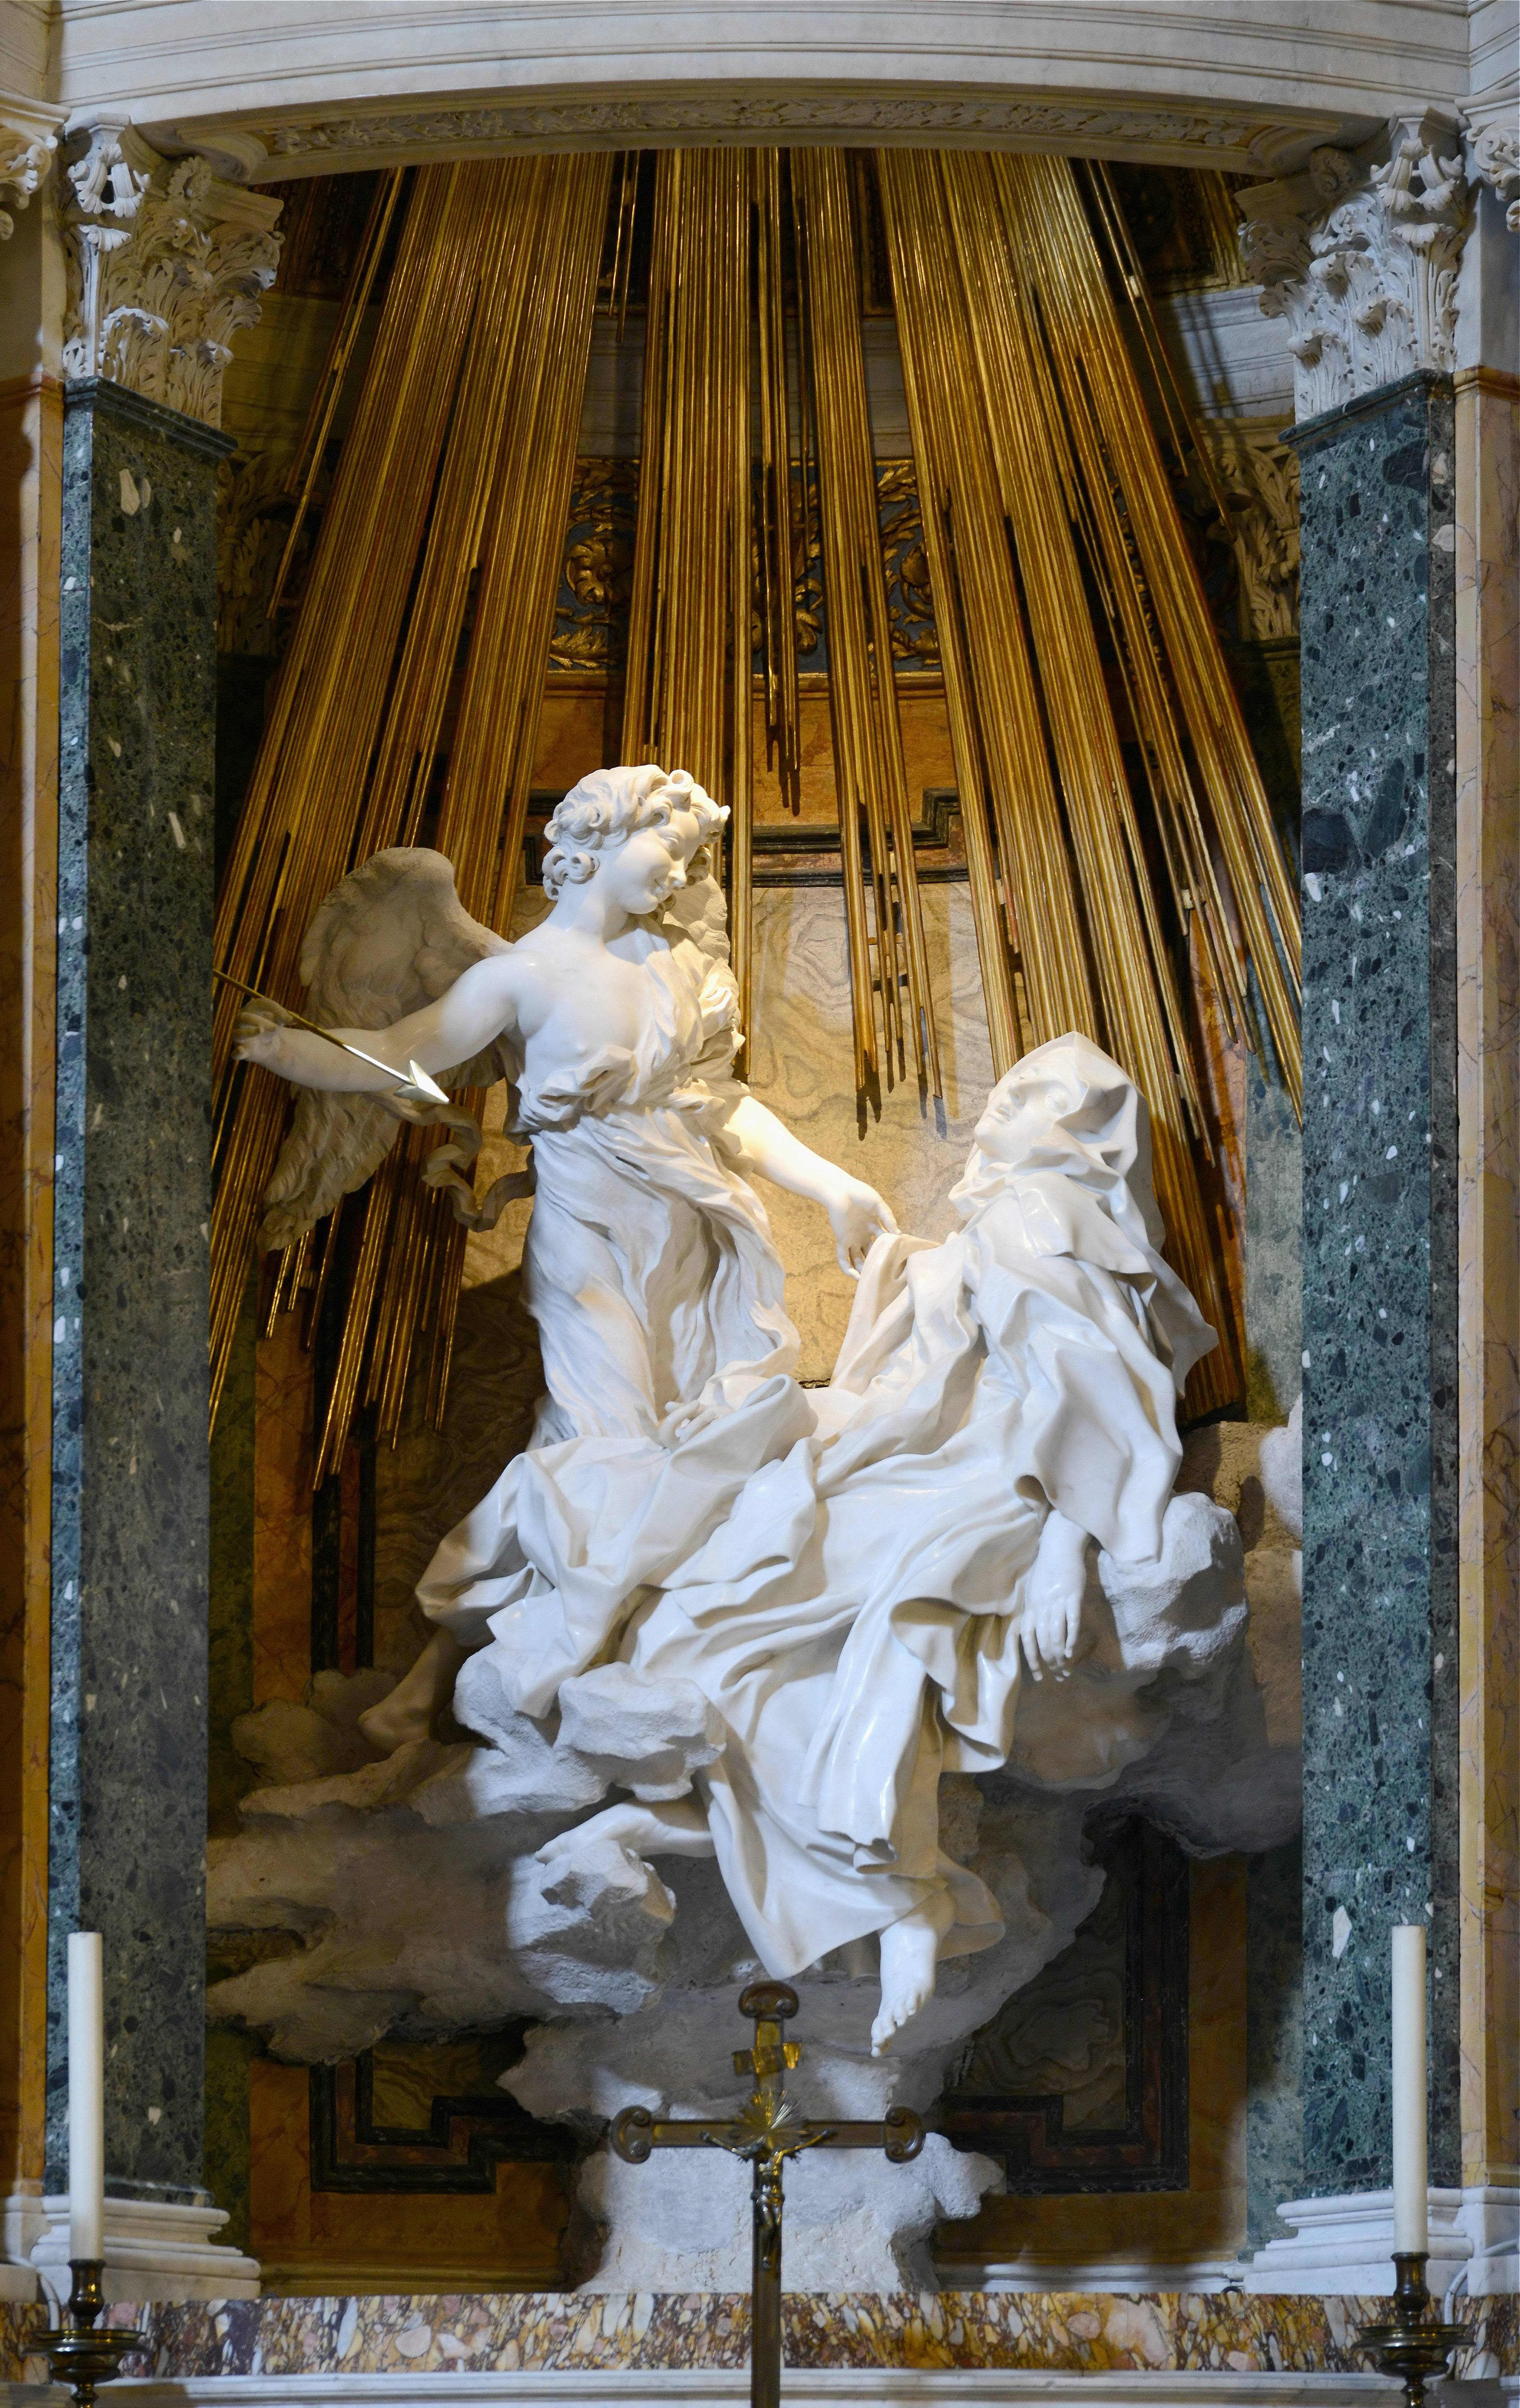
\includegraphics[width=\textwidth]{figura_9.1}
\caption{Rio Tejo}
\label{fig:mesh9.1}
\end{figure}

\newpage

\begin{figure}[h]
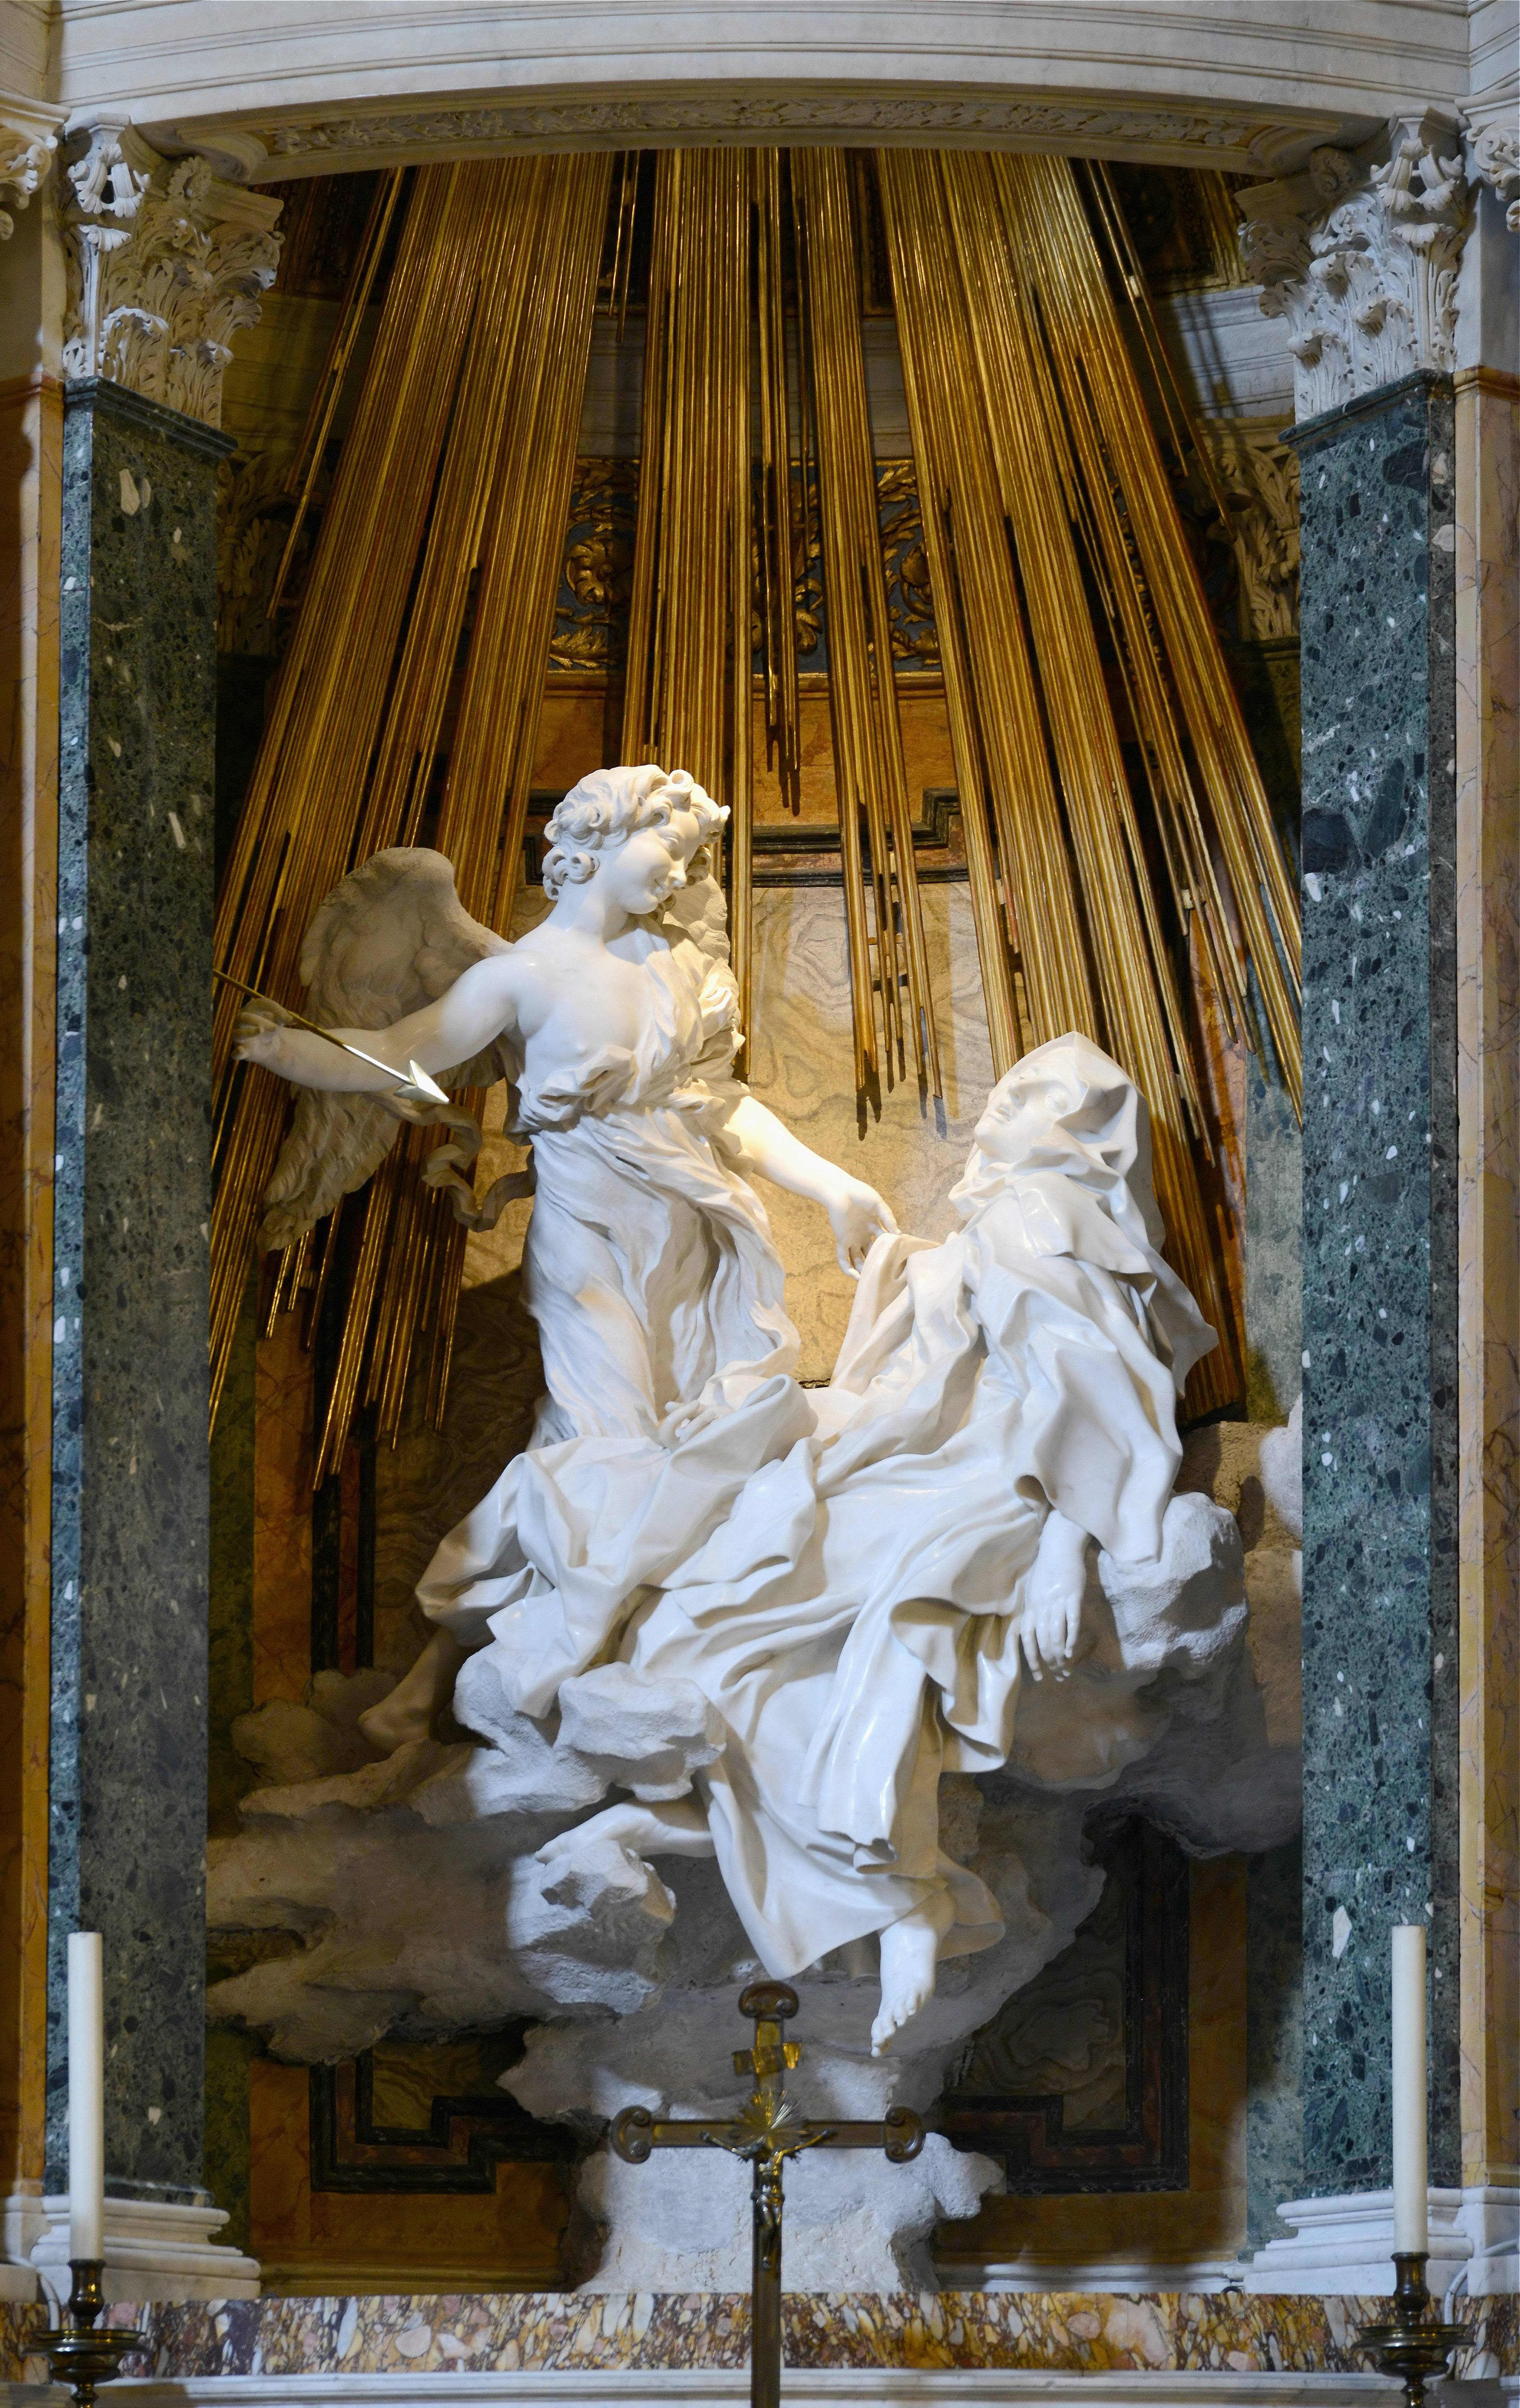
\includegraphics[width=\textwidth]{figura_9.2}
\caption{Ribeirão do Carmo}
\label{fig:mesh9.2}
\end{figure}

\newpage

\begin{figure}[h]
\includegraphics[width=\textwidth]{figura_10.1}
\caption{\textit{A Liberdade guiando o povo}, de Eugène Delacroix. 1830}
\label{fig:mesh10.1}
\end{figure}

Note que a figura da Liberdade utiliza um barrete frígio, que representa a república (também a forma como a questão reformista aparecia nas artes plásticas).

\newpage

\begin{figure}[h]
\includegraphics[width=\textwidth]{figura_22.1}
\caption{\textit{A redenção de Cam}, de Modesto Brocos. 1895}
\label{fig:mesh22.1}
\end{figure}

No contexto do Naturalismo no Brasil, o quadro exemplifica de maneira clara a ideia de apuração do sangue. Sob o viés cientificista da época, as mulheres negras teriam um instinto em se relacionar com homens brancos — melhor patrimônio genético, como um macho de raça superior. No contexto brasileiro, buscava-se a maior branquitude possível da população.

\newpage

\begin{figure}[h]
\includegraphics[width=\textwidth]{figura_28.1}
\caption{\textit{Les Demoiselles d'Avignon}, de Pablo Picasso. 1907}
\label{fig:mesh28.1}
\end{figure}

Algum texto aqui.

\newpage

\begin{figure}[h]
\includegraphics[width=\textwidth]{figura_28.2}
\caption{\textit{Frineia em frente ao Areóago}, de Jean-Léon Gerôme. 1861}
\label{fig:mesh28.2}
\end{figure}

Obra contemporânea que retrata o episódio do julgamento de Frineia. Assim como em \textit{O nascimento de Vênus}, os braços levantados possibilitam maior destaque na representação dos seis.

\newpage

\begin{figure}[h]
\includegraphics[width=\textwidth]{figura_28.3}
\caption{\textit{Olympia}, de Édouard Manet. 1863}
\label{fig:mesh28.3}
\end{figure}

Algum texto aqui.

\newpage

\begin{figure}[h]
\includegraphics[width=\textwidth]{figura_28.4}
\caption{\textit{L'Origine du monde}, de Gustave Courbet. 1866}
\label{fig:mesh28.4}
\end{figure}

\newpage

\begin{figure}[h]
\includegraphics[width=\textwidth]{figura_28.5}
\caption{\textit{Retrato da mãe do artista}, de Pablo Picasso. 1896}
\label{fig:mesh28.5}
\end{figure}

Algum texto aqui.

\newpage

\begin{figure}[h]
\includegraphics[width=\textwidth]{figura_28.6}
\caption{\textit{Campo de trigo com corvos}, de Vincent van Gogh. 1890}
\label{fig:mesh28.6}
\end{figure}

Algum texto aqui.

\newpage

\begin{figure}[h]
\includegraphics[width=\textwidth]{figura_28.7}
\caption{\textit{Mont Sainte-Victoire}, de Paul Cézanne. 1904-1906}
\label{fig:mesh28.7}
\end{figure}

Algum texto aqui.

\newpage

\begin{figure}[h]
\includegraphics[width=\textwidth]{figura_28.8}
\caption{\textit{San Giorgio Maggiore au crépuscule'}, de Claude Monet. 1908}
\label{fig:mesh28.8}
\end{figure}

Algum texto aqui.

\newpage

\begin{figure}[h]
\includegraphics[width=\textwidth]{figura_28.9}
\caption{\textit{O grito}, de Edvard Munch. 1893}
\label{fig:mesh28.9}
\end{figure}

Algum texto aqui.

\newpage

\begin{figure}[h]
\includegraphics[width=\textwidth]{figura_28.10}
\caption{\textit{Sick transit}, de José Paulo Paes. 1973}
\label{fig:mesh28.10}
\end{figure}

Algum texto aqui.

\newpage

\begin{figure}[h]
\includegraphics[width=\textwidth]{figura_28.11}
\caption{\textit{Fonte}, de Marcel Duchamp. 1917}
\label{fig:mesh28.11}
\end{figure}

Algum texto aqui. % CADERNO DE IMAGENS

%----------------------------------------------------------------------------------------
%	BIBLIOGRAFIA
%----------------------------------------------------------------------------------------

\chapter*{Bibliografia}
\addcontentsline{toc}{chapter}{\textcolor{ocre}{Bibliografia}}
\section*{Livros}
\addcontentsline{toc}{section}{Books}
\printbibliography[heading=bibempty,type=book]
\section*{Artigos}
\addcontentsline{toc}{section}{Articles}
\printbibliography[heading=bibempty,type=article]

%----------------------------------------------------------------------------------------
%	ÍNDICE
%----------------------------------------------------------------------------------------

\cleardoublepage
\phantomsection
\setlength{\columnsep}{0.75cm}
\addcontentsline{toc}{chapter}{\textcolor{ocre}{Índice}}
\printindex

\end{document}